\documentclass[]{book}
\usepackage{lmodern}
\usepackage{amssymb,amsmath}
\usepackage{ifxetex,ifluatex}
\usepackage{fixltx2e} % provides \textsubscript
\ifnum 0\ifxetex 1\fi\ifluatex 1\fi=0 % if pdftex
  \usepackage[T1]{fontenc}
  \usepackage[utf8]{inputenc}
\else % if luatex or xelatex
  \ifxetex
    \usepackage{mathspec}
  \else
    \usepackage{fontspec}
  \fi
  \defaultfontfeatures{Ligatures=TeX,Scale=MatchLowercase}
\fi
% use upquote if available, for straight quotes in verbatim environments
\IfFileExists{upquote.sty}{\usepackage{upquote}}{}
% use microtype if available
\IfFileExists{microtype.sty}{%
\usepackage{microtype}
\UseMicrotypeSet[protrusion]{basicmath} % disable protrusion for tt fonts
}{}
\usepackage[margin=1in]{geometry}
\usepackage{hyperref}
\hypersetup{unicode=true,
            pdftitle={FARM: simulating the spread of agriculture through cultural phylogenies},
            pdfauthor={Ty Tuff, Bruno Vilela, and Carlos Botero},
            pdfborder={0 0 0},
            breaklinks=true}
\urlstyle{same}  % don't use monospace font for urls
\usepackage{natbib}
\bibliographystyle{apalike}
\usepackage{color}
\usepackage{fancyvrb}
\newcommand{\VerbBar}{|}
\newcommand{\VERB}{\Verb[commandchars=\\\{\}]}
\DefineVerbatimEnvironment{Highlighting}{Verbatim}{commandchars=\\\{\}}
% Add ',fontsize=\small' for more characters per line
\usepackage{framed}
\definecolor{shadecolor}{RGB}{248,248,248}
\newenvironment{Shaded}{\begin{snugshade}}{\end{snugshade}}
\newcommand{\KeywordTok}[1]{\textcolor[rgb]{0.13,0.29,0.53}{\textbf{{#1}}}}
\newcommand{\DataTypeTok}[1]{\textcolor[rgb]{0.13,0.29,0.53}{{#1}}}
\newcommand{\DecValTok}[1]{\textcolor[rgb]{0.00,0.00,0.81}{{#1}}}
\newcommand{\BaseNTok}[1]{\textcolor[rgb]{0.00,0.00,0.81}{{#1}}}
\newcommand{\FloatTok}[1]{\textcolor[rgb]{0.00,0.00,0.81}{{#1}}}
\newcommand{\ConstantTok}[1]{\textcolor[rgb]{0.00,0.00,0.00}{{#1}}}
\newcommand{\CharTok}[1]{\textcolor[rgb]{0.31,0.60,0.02}{{#1}}}
\newcommand{\SpecialCharTok}[1]{\textcolor[rgb]{0.00,0.00,0.00}{{#1}}}
\newcommand{\StringTok}[1]{\textcolor[rgb]{0.31,0.60,0.02}{{#1}}}
\newcommand{\VerbatimStringTok}[1]{\textcolor[rgb]{0.31,0.60,0.02}{{#1}}}
\newcommand{\SpecialStringTok}[1]{\textcolor[rgb]{0.31,0.60,0.02}{{#1}}}
\newcommand{\ImportTok}[1]{{#1}}
\newcommand{\CommentTok}[1]{\textcolor[rgb]{0.56,0.35,0.01}{\textit{{#1}}}}
\newcommand{\DocumentationTok}[1]{\textcolor[rgb]{0.56,0.35,0.01}{\textbf{\textit{{#1}}}}}
\newcommand{\AnnotationTok}[1]{\textcolor[rgb]{0.56,0.35,0.01}{\textbf{\textit{{#1}}}}}
\newcommand{\CommentVarTok}[1]{\textcolor[rgb]{0.56,0.35,0.01}{\textbf{\textit{{#1}}}}}
\newcommand{\OtherTok}[1]{\textcolor[rgb]{0.56,0.35,0.01}{{#1}}}
\newcommand{\FunctionTok}[1]{\textcolor[rgb]{0.00,0.00,0.00}{{#1}}}
\newcommand{\VariableTok}[1]{\textcolor[rgb]{0.00,0.00,0.00}{{#1}}}
\newcommand{\ControlFlowTok}[1]{\textcolor[rgb]{0.13,0.29,0.53}{\textbf{{#1}}}}
\newcommand{\OperatorTok}[1]{\textcolor[rgb]{0.81,0.36,0.00}{\textbf{{#1}}}}
\newcommand{\BuiltInTok}[1]{{#1}}
\newcommand{\ExtensionTok}[1]{{#1}}
\newcommand{\PreprocessorTok}[1]{\textcolor[rgb]{0.56,0.35,0.01}{\textit{{#1}}}}
\newcommand{\AttributeTok}[1]{\textcolor[rgb]{0.77,0.63,0.00}{{#1}}}
\newcommand{\RegionMarkerTok}[1]{{#1}}
\newcommand{\InformationTok}[1]{\textcolor[rgb]{0.56,0.35,0.01}{\textbf{\textit{{#1}}}}}
\newcommand{\WarningTok}[1]{\textcolor[rgb]{0.56,0.35,0.01}{\textbf{\textit{{#1}}}}}
\newcommand{\AlertTok}[1]{\textcolor[rgb]{0.94,0.16,0.16}{{#1}}}
\newcommand{\ErrorTok}[1]{\textcolor[rgb]{0.64,0.00,0.00}{\textbf{{#1}}}}
\newcommand{\NormalTok}[1]{{#1}}
\usepackage{longtable,booktabs}
\usepackage{graphicx,grffile}
\makeatletter
\def\maxwidth{\ifdim\Gin@nat@width>\linewidth\linewidth\else\Gin@nat@width\fi}
\def\maxheight{\ifdim\Gin@nat@height>\textheight\textheight\else\Gin@nat@height\fi}
\makeatother
% Scale images if necessary, so that they will not overflow the page
% margins by default, and it is still possible to overwrite the defaults
% using explicit options in \includegraphics[width, height, ...]{}
\setkeys{Gin}{width=\maxwidth,height=\maxheight,keepaspectratio}
\IfFileExists{parskip.sty}{%
\usepackage{parskip}
}{% else
\setlength{\parindent}{0pt}
\setlength{\parskip}{6pt plus 2pt minus 1pt}
}
\setlength{\emergencystretch}{3em}  % prevent overfull lines
\providecommand{\tightlist}{%
  \setlength{\itemsep}{0pt}\setlength{\parskip}{0pt}}
\setcounter{secnumdepth}{5}
% Redefines (sub)paragraphs to behave more like sections
\ifx\paragraph\undefined\else
\let\oldparagraph\paragraph
\renewcommand{\paragraph}[1]{\oldparagraph{#1}\mbox{}}
\fi
\ifx\subparagraph\undefined\else
\let\oldsubparagraph\subparagraph
\renewcommand{\subparagraph}[1]{\oldsubparagraph{#1}\mbox{}}
\fi

%%% Use protect on footnotes to avoid problems with footnotes in titles
\let\rmarkdownfootnote\footnote%
\def\footnote{\protect\rmarkdownfootnote}

%%% Change title format to be more compact
\usepackage{titling}

% Create subtitle command for use in maketitle
\newcommand{\subtitle}[1]{
  \posttitle{
    \begin{center}\large#1\end{center}
    }
}

\setlength{\droptitle}{-2em}
  \title{FARM: simulating the spread of agriculture through cultural phylogenies}
  \pretitle{\vspace{\droptitle}\centering\huge}
  \posttitle{\par}
\subtitle{Users manual for running simulations in R and on Linux clusters}
  \author{Ty Tuff, Bruno Vilela, and Carlos Botero}
  \preauthor{\centering\large\emph}
  \postauthor{\par}
  \predate{\centering\large\emph}
  \postdate{\par}
  \date{project began: 15 May 2016, document updated: 06 February 2018}

\usepackage{booktabs}
\usepackage{amsthm}
\makeatletter
\def\thm@space@setup{%
  \thm@preskip=8pt plus 2pt minus 4pt
  \thm@postskip=\thm@preskip
}
\makeatother

\usepackage{amsthm}
\newtheorem{theorem}{Theorem}[chapter]
\newtheorem{lemma}{Lemma}[chapter]
\theoremstyle{definition}
\newtheorem{definition}{Definition}[chapter]
\newtheorem{corollary}{Corollary}[chapter]
\newtheorem{proposition}{Proposition}[chapter]
\theoremstyle{definition}
\newtheorem{example}{Example}[chapter]
\theoremstyle{definition}
\newtheorem{exercise}{Exercise}[chapter]
\theoremstyle{remark}
\newtheorem*{remark}{Remark}
\newtheorem*{solution}{Solution}
\begin{document}
\maketitle

{
\setcounter{tocdepth}{1}
\tableofcontents
}
\chapter{Introduction}\label{introduction}

While we have information on where nodes should be located, we still
lack data on how cultural nodes should be connected. To compensate for a
lack of data describing these connections between societies, we
randomized the number of edges between nodes for different simulations.
We created 11 different networks, each with a different minimum number
of neighbors ranging from 4 to 14 computed using the function \ldots{}
in the R package \ldots{} . This function builds a network where the
minimum number of connections is achieved for every node, but some nodes
may have more connections than that minimum in order to achieve the
minimum connections for every node across the network. At the beginning
of each simulation, the algorithm draws one of the 11 available networks
and uses that network as the arena for carrying out that simulation.

Each node occupies a unique geographic location that is assigned a
binary value indicating whether the environment of the region is more
favorable to foragers or domesticators based on the results from Vilela
et al (unpublished work). This designation was determined by the
potential richness of domesticated species in each location estimated
using ecological niche models. The threshold richness, above which we
considered the region more favorable to domesticators, correspond to the
potential number of species where farming societies become the dominant
form of subsistence. Only some of these societies were inside of the
known origins of agriculture as reported by Larson et al 2014 so, we
assigned each node a value of 1 or 0 to distinguish between those inside
or outside of those origins.

\chapter{Spatial scaffolding for the
simulations}\label{spatial-scaffolding-for-the-simulations}

Using the \textasciitilde{}8000 currently extant cultures cataloged in
the glottolog repository (\url{http://glottolog.org}), we calculated a
symetrical spatial proximity network connecting them. This network
provides the scaffolding for the simulation to grow on.

\begin{Shaded}
\begin{Highlighting}[]
\KeywordTok{library}\NormalTok{(FARM)}
\KeywordTok{library}\NormalTok{(spdep)}
\KeywordTok{library}\NormalTok{(geosphere)}
\KeywordTok{library}\NormalTok{(maps)}
\end{Highlighting}
\end{Shaded}

We constructed this network using the functions knearneigh() and
knn2nb() in the package spdep. The user identifies the number of
neighbors and the algorythm identifies that many nearest neighbors
calculated based on proximity. Using those neighbor identifiers, we then
calculated the great circle distance between each point using the
gcIntermediate() function from the geosphere package and ploted those
lines over a map.

Through a seperate analysis based on ecological niche models of
agricultue, we determined that networks with 7 neighbors produced
spatial distributions with the lowest level of autocorrelation.
Accordingly, we ran the simulation on networks with 5-9 connections
between neighbors to represent some variation in this parameter but
centered these estimates around 7. At the begining of each simualation,
one network was chosen from the 5 possible arrangements and used as
simulation scaffolding. The number of neighbors assigned to a particular
simulation replicate is recorded in the metadata so it can be extracted
and used as a covariate in later models.

Here is the code for producing and plotting these networks. The object
language\_centroids is in the FARM package, so make sure that package is
loaded so R can find the required data. Below the code are plots of the
5 possible graph arrangements used in the FARM simulations.

\begin{Shaded}
\begin{Highlighting}[]
\NormalTok{coords <-}\StringTok{ }\KeywordTok{as.matrix}\NormalTok{(}\KeywordTok{apply}\NormalTok{(language_centroids[, }\DecValTok{3}\OperatorTok{:}\DecValTok{4}\NormalTok{], }\DecValTok{2}\NormalTok{, as.numeric)) }\CommentTok{#coords}
\NormalTok{conds <-}\StringTok{ }\KeywordTok{ifelse}\NormalTok{(suitability2 }\OperatorTok{==}\StringTok{ }\DecValTok{0}\NormalTok{, }\DecValTok{1}\NormalTok{, }\DecValTok{2}\NormalTok{)}
\NormalTok{conds[}\KeywordTok{is.na}\NormalTok{(conds)] <-}\StringTok{ }\KeywordTok{sample}\NormalTok{(}\KeywordTok{c}\NormalTok{(}\DecValTok{1}\NormalTok{, }\DecValTok{2}\NormalTok{), }\KeywordTok{sum}\NormalTok{(}\KeywordTok{is.na}\NormalTok{(conds)), }\DataTypeTok{replace =} \OtherTok{TRUE}\NormalTok{) }
\NormalTok{origins <-}\StringTok{ }\NormalTok{language_centroids[, }\DecValTok{5}\NormalTok{]}



\NormalTok{nbs_number <-}\StringTok{ }\DecValTok{2}
\NormalTok{this_row <-}\StringTok{ }\DecValTok{1}
\NormalTok{number_of_neighbors <-}\StringTok{ }\DecValTok{7}
\ControlFlowTok{for}\NormalTok{(i }\ControlFlowTok{in} \DecValTok{5}\OperatorTok{:}\DecValTok{9}\NormalTok{)\{}

\NormalTok{number_of_neighbors <-}\StringTok{ }\NormalTok{i}
\NormalTok{nbs <-}\StringTok{ }\KeywordTok{knearneigh}\NormalTok{(coords, }\DataTypeTok{k =}\NormalTok{ number_of_neighbors, }\DataTypeTok{longlat =} \OtherTok{TRUE}\NormalTok{) }

\NormalTok{nbs_list <-}\StringTok{ }\KeywordTok{knn2nb}\NormalTok{(nbs, }\DataTypeTok{sym =} \OtherTok{TRUE}\NormalTok{)}


\KeywordTok{png}\NormalTok{(}\KeywordTok{paste}\NormalTok{(}\StringTok{"network_scratch_"}\NormalTok{, number_of_neighbors, }\StringTok{".png"}\NormalTok{), }\DataTypeTok{width=}\DecValTok{11}\NormalTok{, }\DataTypeTok{height=}\FloatTok{5.5}\NormalTok{, }\DataTypeTok{res=}\DecValTok{1000}\NormalTok{, }\DataTypeTok{units =} \StringTok{"in"}\NormalTok{)}


\KeywordTok{par}\NormalTok{(}\DataTypeTok{mar=}\KeywordTok{c}\NormalTok{(}\DecValTok{0}\NormalTok{,}\DecValTok{0}\NormalTok{,}\DecValTok{0}\NormalTok{,}\DecValTok{0}\NormalTok{))}

\KeywordTok{plot}\NormalTok{(}\DecValTok{0}\NormalTok{,}\DecValTok{0}\NormalTok{, }\DataTypeTok{xlim=}\KeywordTok{c}\NormalTok{(}\OperatorTok{-}\DecValTok{180}\NormalTok{,}\DecValTok{180}\NormalTok{), }\DataTypeTok{ylim=}\KeywordTok{c}\NormalTok{(}\OperatorTok{-}\DecValTok{90}\NormalTok{,}\DecValTok{90}\NormalTok{), }\DataTypeTok{type=}\StringTok{"n"}\NormalTok{)}
\KeywordTok{map}\NormalTok{(}\StringTok{"world"}\NormalTok{, }\DataTypeTok{col=}\KeywordTok{adjustcolor}\NormalTok{(}\StringTok{"lightgrey"}\NormalTok{, }\DataTypeTok{alpha=}\FloatTok{0.2}\NormalTok{), }\DataTypeTok{interior =} \OtherTok{FALSE}\NormalTok{, }\DataTypeTok{fill=}\OtherTok{TRUE}\NormalTok{, }\DataTypeTok{border=}\OtherTok{NA}\NormalTok{)}
\CommentTok{#map("state", col="lightgrey")}
\ControlFlowTok{for}\NormalTok{(this_row }\ControlFlowTok{in} \DecValTok{1}\OperatorTok{:}\KeywordTok{length}\NormalTok{(nbs_list))\{}
\ControlFlowTok{for}\NormalTok{(nbs_number }\ControlFlowTok{in} \DecValTok{1}\OperatorTok{:}\KeywordTok{length}\NormalTok{(nbs_list[[this_row]]))\{}
\CommentTok{#pointser <- NULL}
\NormalTok{pointser <-}\StringTok{ }\KeywordTok{gcIntermediate}\NormalTok{(}\KeywordTok{c}\NormalTok{(coords[nbs_list[[this_row]][nbs_number],}\DecValTok{1}\NormalTok{], coords[nbs_list[[this_row]][nbs_number],}\DecValTok{2}\NormalTok{]), }\KeywordTok{c}\NormalTok{(coords[this_row,}\DecValTok{1}\NormalTok{], coords[this_row,}\DecValTok{2}\NormalTok{]), }\DataTypeTok{n=}\DecValTok{100}\NormalTok{, }\DataTypeTok{breakAtDateLine =}\NormalTok{ T)}
    \KeywordTok{length}\NormalTok{(pointser)}
        \ControlFlowTok{if}\NormalTok{(}\KeywordTok{length}\NormalTok{(pointser) }\OperatorTok{==}\StringTok{ }\DecValTok{200}\NormalTok{)\{}\KeywordTok{lines}\NormalTok{(pointser, }\DataTypeTok{col=}\KeywordTok{adjustcolor}\NormalTok{(}\StringTok{"black"}\NormalTok{, }\DataTypeTok{alpha=}\DecValTok{1}\NormalTok{), }\DataTypeTok{lwd=}\NormalTok{.}\DecValTok{3}\NormalTok{)\}}
\ControlFlowTok{if}\NormalTok{(}\KeywordTok{length}\NormalTok{(pointser) }\OperatorTok{==}\StringTok{ }\DecValTok{2}\NormalTok{)\{}\KeywordTok{lines}\NormalTok{(pointser[[}\DecValTok{1}\NormalTok{]], }\DataTypeTok{col=}\KeywordTok{adjustcolor}\NormalTok{(}\StringTok{"black"}\NormalTok{, }\DataTypeTok{alpha=}\DecValTok{1}\NormalTok{), }\DataTypeTok{lwd=}\NormalTok{.}\DecValTok{3}\NormalTok{)}
    \KeywordTok{lines}\NormalTok{(pointser[[}\DecValTok{2}\NormalTok{]], }\DataTypeTok{col=}\KeywordTok{adjustcolor}\NormalTok{(}\StringTok{"black"}\NormalTok{, }\DataTypeTok{alpha=}\DecValTok{1}\NormalTok{), }\DataTypeTok{lwd=}\NormalTok{.}\DecValTok{3}\NormalTok{)\}}
    
    \CommentTok{#lines(pointser, col="red", lwd=.5)}
\ControlFlowTok{if}\NormalTok{(}\KeywordTok{length}\NormalTok{(pointser) }\OperatorTok{==}\StringTok{ }\DecValTok{200}\NormalTok{)\{}\KeywordTok{lines}\NormalTok{(pointser, }\DataTypeTok{col=}\StringTok{"cornflowerblue"}\NormalTok{, }\DataTypeTok{lwd=}\NormalTok{.}\DecValTok{25}\NormalTok{)\}}
\ControlFlowTok{if}\NormalTok{(}\KeywordTok{length}\NormalTok{(pointser) }\OperatorTok{==}\StringTok{ }\DecValTok{2}\NormalTok{)\{}\KeywordTok{lines}\NormalTok{(pointser[[}\DecValTok{1}\NormalTok{]], }\DataTypeTok{col=}\StringTok{"cornflowerblue"}\NormalTok{, }\DataTypeTok{lwd=}\NormalTok{.}\DecValTok{25}\NormalTok{)}
    \KeywordTok{lines}\NormalTok{(pointser[[}\DecValTok{2}\NormalTok{]], }\DataTypeTok{col=}\StringTok{"cornflowerblue"}\NormalTok{, }\DataTypeTok{lwd=}\NormalTok{.}\DecValTok{25}\NormalTok{)\}}
    

    \KeywordTok{mtext}\NormalTok{(}\KeywordTok{paste0}\NormalTok{(}\StringTok{"Network with at least "}\NormalTok{, number_of_neighbors, }\StringTok{" connections between each culture"}\NormalTok{), }\DecValTok{3}\NormalTok{, }\DataTypeTok{line=}\DecValTok{0}\NormalTok{)}
\NormalTok{\}\}}

\KeywordTok{dev.off}\NormalTok{()}


\NormalTok{\}}
\end{Highlighting}
\end{Shaded}

\includegraphics{network_scratch_ 5 .png}
\includegraphics{network_scratch_ 6 .png}
\includegraphics{network_scratch_ 7 .png}

\includegraphics{network_scratch_ 8 .png}
\includegraphics{network_scratch_ 9 .png}

\chapter{Rule sets}\label{rule-sets}

\begin{verbatim}
## 
## The downloaded binary packages are in
##  /var/folders/4v/qwc_jrrd1wd07klywdz9qv8c0000gq/T//RtmpMihxdG/downloaded_packages
\end{verbatim}

\begin{verbatim}
## 
## The downloaded binary packages are in
##  /var/folders/4v/qwc_jrrd1wd07klywdz9qv8c0000gq/T//RtmpMihxdG/downloaded_packages
\end{verbatim}

\begin{verbatim}
## 
## The downloaded binary packages are in
##  /var/folders/4v/qwc_jrrd1wd07klywdz9qv8c0000gq/T//RtmpMihxdG/downloaded_packages
\end{verbatim}

\section{Simulation:}\label{simulation}

Building a model that simulates the spread of agriculture across human
cultures took several independently built and validated components. The
simulations play out in an arena defined by a spatial network of
cultural centroids and those networks needed to be defined. Assigning
agricultural suitability measures to each society required first
modeling agricultural suitability across all environments and then
assigning suitability values to each node in the spatial network. Events
unfold as simulations progress through time and those events must be
tracked from beginning to end. Running these simulations required the
development of a stand-alone system for generating input parameters that
control the experimental design. Rules for how simulations operate were
carefully designed to describe the behavior of each hypothesized
mechanism. Each replicate simulation produced a spatial pattern and
phylogenetic tree that are too complex to compare to each other directly
so, each simulation output is summarized by 12 summary statistics that
can be passed to the random forest machine learning algorithm for
categorization. These six components each play an important role in the
design and operation such a large-scale simulation. We describe each
component of the simulation in more detail below.

There are 5 general behavioral continuation rules that correspond to the
5 categories of input variables described above. The first 3 rules are
included in all models. Rules 4 and 5 are either included or excluded
from the model to define different model types corresponding to
different hypothesized mechanisms. These rules describe the possible
ways that each node can change status (e.g.~change from or to extant,
extinct, forager, or domesticator) over the course of one time step and
we define them as follows:

\subsubsection{1. Arisal -}\label{arisal--}

A society switches their subsistence mode without any influence from
ancestors or neighbors.

\subsubsection{2. Extinction -}\label{extinction--}

A society dies out. This terminates their branch of the phylogeny and
resets their node to unoccupied. The probability of extinction is higher
when the society's subsistence mode doesn't match their environment.

\subsubsection{3. Speciation -}\label{speciation--}

A society expands spatially across the network by sending a descendent
diaspora to colonize an unoccupied adjoining node. This expansion into
unoccupied territory creates a speciation event, where a new branch is
added to the phylogeny showing a new society as a descendent of th e
original society. If all adjoining nodes are occupied, then speciation
cannot occur. The decedent society inherits their subsistence mode from
the parent society, regardless of environment.

\subsubsection{4. Diffusion -}\label{diffusion--}

A society converts an occupied adjoining society to match its own
subsistence mode. If there are no occupied neighboring nodes with an
opposing subsistence mode, then diffusion cannot occur.

\subsubsection{5. Takeover -}\label{takeover--}

A society expands spatially across the network by sending a descendent
diaspora to colonize an occupied adjoining node. If the target society
is connected to an unoccupied node, then that society can flee this
expansion and avoid extinction by abandoning their current node and
colonizing that unoccupied node. If the target society is surrounded by
occupied nodes, then they will go extinct when the expanding society
colonizes their node. This extinction terminates their branch of the
phylogeny and resets their spatial node to unoccupied. As with
speciation, the expansion of the conquering society's diaspora creates a
speciation event, where a new branch is added to the phylogeny showing a
new society as a descendent of the original society. If all adjoining
nodes are unoccupied, then takeover cannot occur. The decedent society
of the conquer inherits their subsistence mode from the parent society,
regardless of environment.

To avoid any implied hierarchy between these rules or between nodes,
both were randomized regularly. Within a single time step, the order of
the rules were randomized before applying them to any nodes and then
they were applied one-rule-at-a-time randomly (sampled without
replacement) across all the nodes. One time step was complete when all
the rules had been applied to all of the individual nodes. When one time
step turns over to another, the order of rules is redrawn and they are
again applied randomly across the nodes. This process was repeated for
30,000 time steps, which preliminary experiments showed was long enough
for the system to reach equilibrium. Using preliminary trials of the
simulations, we concluded that the model had reached equilibrium by
plotting summary statistics through time and showing that statistics
that asymptote usually do so between 10 and 20 thousand time steps so
they are stabilized well before 30,000 time steps.

\begin{figure}
\centering
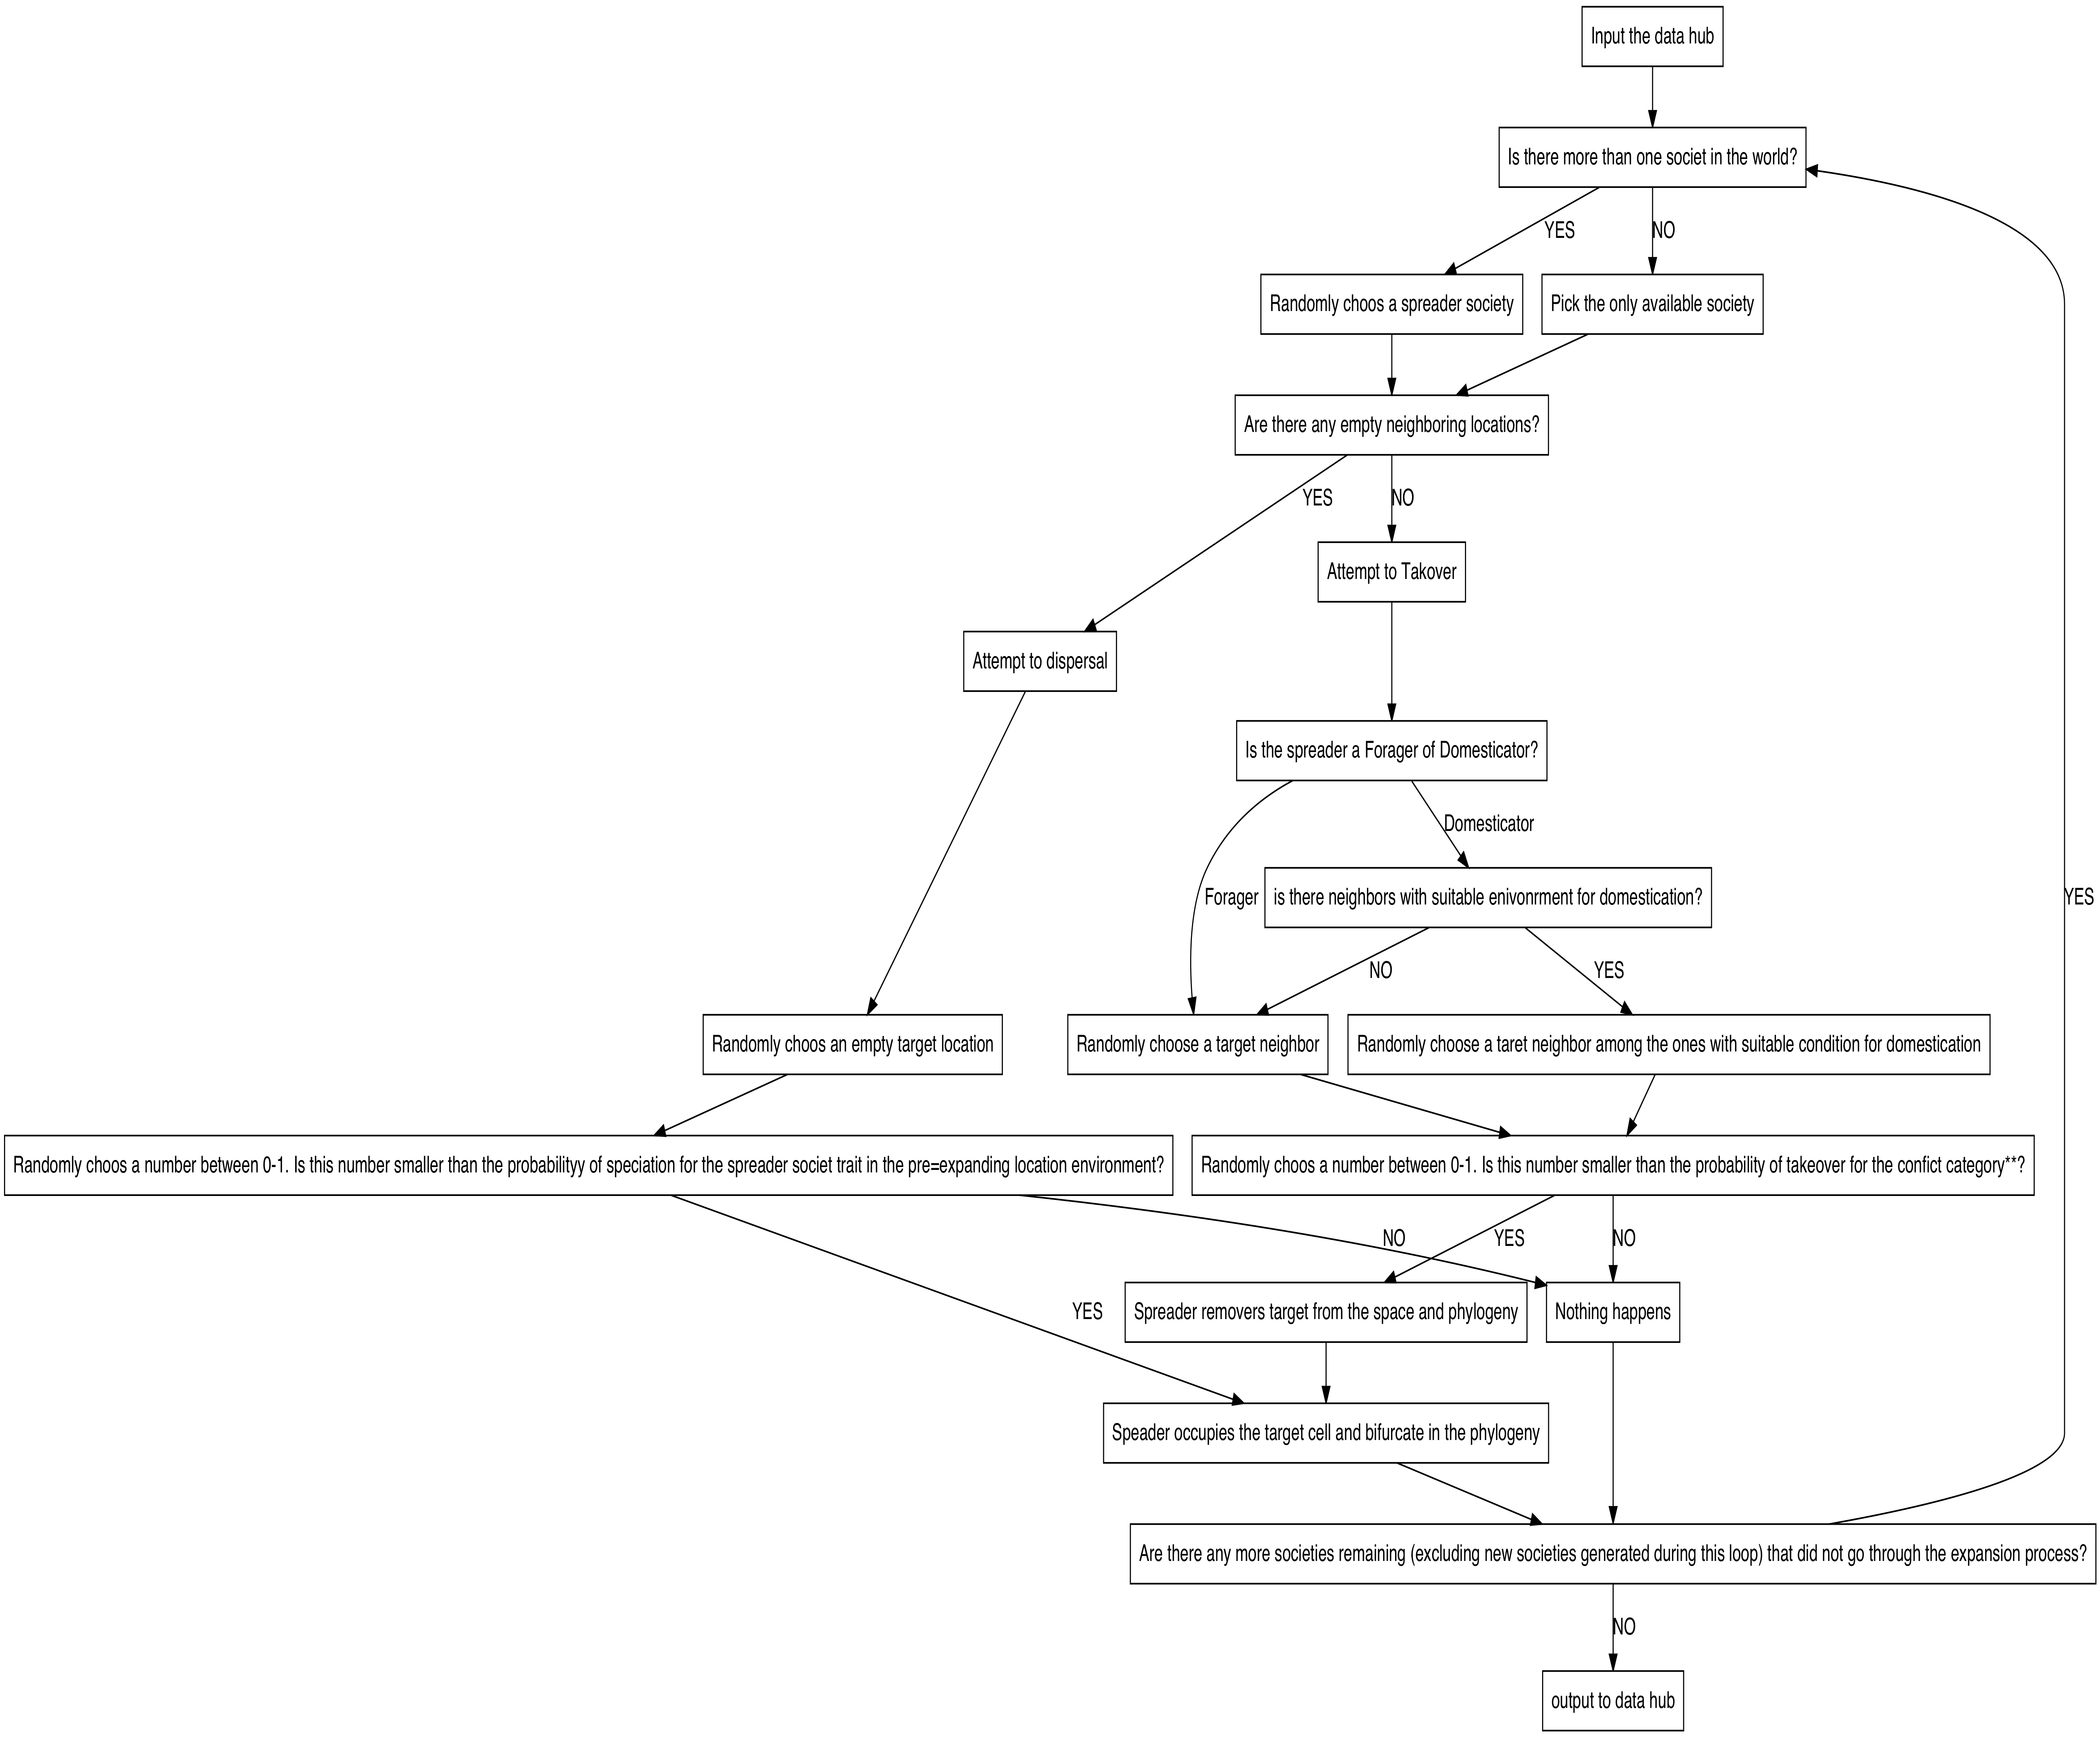
\includegraphics{stnds.qa.png}
\caption{Rule set for the Takeover model}
\end{figure}

```

\chapter{Module 1: Simulation to produce a world and a
tree}\label{module-1-simulation-to-produce-a-world-and-a-tree}

After the spatial network was built to host the simulations, the
machinery for tracking simulation progress was in place, and the input
parameters were assigned, then each simulation could launch according to
a set of initial launch rules and then play out according to a separate
set of continuing behavioral rules. The initial launch rules begin by
stipulating that the first human culture will originate within
modern-day Ethiopia and radiate outward from that point. All of these
original cultures use foraging as their only mode of subsistence until
at least 80\% of the available nodes are occupied by a culture and then
agriculture can start to arise by foragers switching to
agriculturalists. The ability to switch from forager to agriculturalist
without any outside influence is restricted to within known origins of
agriculture as defined by Larson et al. (2014). Switching from forager
to agriculturalist can only occur on nodes within those known origins,
but agriculturalists can switch to foragers with equal probability on
any node. Nodes can only interact via edges so, edges define neighboring
nodes. These initial launch rules are the same for all simulations,
regardless of the hypothesized mechanism they are simulating.

When simulations were terminated at 30,000 time steps, they will have
produced a spatial pattern of subsistence modes distributed across the
geographic network and a phylogeny describing the relatedness of those
societies through time. These two objects contain a great deal of
information about the trajectory of particular replicates but that
complexity makes it difficult to compare replicates directly. No test
currently exists to compare a combination of spatial and phylogenetic
patterns between replicated simulations. To simplify these outputs and
allow them to be compared directly to each other, we calculated a suite
of 12 summary statistics to describe different features of both the
spatial distribution and the phylogeny. During preliminary tests of the
simulations, we used 19 summary statistics but later eliminated 7 of
those original statistics because they didn't stabilize over time to
where they could be described by a linear model. The 12 remaining
statistics stabilized by either increasing regularly through time or
came to an asymptote as the simulation reached equilibrium (SI
figure\ldots{}). After all of the simulations were complete, these
summary statistics were concatenated into a single dataset, labelled
with the rule set (mechanism) used to create each one, and then passed
on to the random forest algorithm for analysis.

\begin{Shaded}
\begin{Highlighting}[]
\CommentTok{# Install the most recent version of FARM from a .zip file}
\KeywordTok{install.packages}\NormalTok{(}\KeywordTok{file.choose}\NormalTok{(), }\DataTypeTok{repos=}\OtherTok{NULL}\NormalTok{) }
\end{Highlighting}
\end{Shaded}

\begin{Shaded}
\begin{Highlighting}[]
\KeywordTok{library}\NormalTok{(FARM)}
\KeywordTok{ls}\NormalTok{(}\StringTok{"package:FARM"}\NormalTok{)}
\end{Highlighting}
\end{Shaded}

\begin{verbatim}
##  [1] "Arisal"                  "bd"                     
##  [3] "BuildWorld"              "combo_of_choice"        
##  [5] "coords"                  "coords.austronisian"    
##  [7] "coords.bantu"            "coords.uto"             
##  [9] "Diffusion"               "DivDep"                 
## [11] "DropTip"                 "Dsig"                   
## [13] "evol.distinct2"          "extinct"                
## [15] "Extinction"              "getTargets"             
## [17] "language_centroids"      "makePhy"                
## [19] "Module_2"                "NewTip"                 
## [21] "parameters"              "parameters.table"       
## [23] "plot.myworld"            "RunSim"                 
## [25] "RunSim.push"             "RunSim2"                
## [27] "RunSim2.push"            "RunSimUltimate"         
## [29] "RunSimUltimate.push"     "RunSimUltimate2"        
## [31] "RunSimUltimate2.push"    "speciate"               
## [33] "Speciation"              "SpeciationTakeOver"     
## [35] "SpeciationTakeOver.push" "sub.TakeOver"           
## [37] "sub.TakeOver.push"       "suitability"            
## [39] "suitability2"            "TakeOver"               
## [41] "TakeOver.push"           "TheOriginOfSpecies"
\end{verbatim}

\section{Inputs}\label{inputs}

The specific behavior of any particular replicate simulation is
controlled by 17 input parameters. All of these values are unique to
each replicate simulation, but don't change from the beginning to the
end of a simulation. These parameters are all constrained between 0 and
1 and fall within five general categories: speciation, extinction,
cultural diffusion, diffusion by takeover, and arisal. The first two
categories, speciation and extinction, each require four parameters to
describe the different ways that farmers and foragers can interact with
environments that are suitable or unsuitable for agriculture. Diffusion
by takeover also requires four parameters to describe the four ways that
farmers or foragers can displace their neighbors to expand their
subsistence mode. Cultural diffusion is simpler than diffusion by
takeover and only requires two input parameters: diffusion from farmers
to foragers and diffusion from foragers to farmers. Arisal follows the
same convention as the cultural diffusion inputs but the probability of
switching from foragers to farmers is constraining to within the known
origins of agriculture (see Figure 2).

Most of the input parameters are drawn randomly from a uniform
distribution constrained between 0 and 1, but some of these uniform
random draws are constrained more narrowly. Parameter values in the
speciation or extinction categories are ordered so that farmers in
environments suitable for farming will have the highest speciation rate
and lowest extinction rate, farmers in environments unsuitable for
agriculture will have the lowest speciation rate and highest extinction
rate, and all foragers will have an intermediate probability between
them. The first value selected during a random draw is assigned to the
high probability input, the second is constrained to be smaller than the
first draw and assigned to the low probability input, the third is
constrained between the first two values. Arisal is constrained so that
the probability of switching from forager to farmer is always higher
than switching from farmer to forager.

The input parameters are also where the model type is assigned to each
simulation. The hypothesized mechanism prescribed to each simulation are
relayed to the algorithm by setting specific sets of parameters to 0 so
certain events have no chance of happening. The full ensemble model
(+culture +takeover) assigns a value to all 17 parameters, the cultural
diffusion only model (+culture) sets all takeover values to 0, the
diffusion by takeover model (+takeover) sets all cultural diffusion
values to 0, and the basic model sets all culture and takeover values to
0.

\section{Module 1 functions}\label{module-1-functions}

\subsubsection{The first set of RunSim functions are the default
pipeline where only one output is saved at the end of the
simulation.}\label{the-first-set-of-runsim-functions-are-the-default-pipeline-where-only-one-output-is-saved-at-the-end-of-the-simulation.}

This first function controls error messages coming from the primary
function below.

\begin{Shaded}
\begin{Highlighting}[]
\CommentTok{# Run the simulation function skiping the erros and atributing NA if it occurs}
\NormalTok{RunSimUltimate <-}\StringTok{ }\ControlFlowTok{function}\NormalTok{(myWorld, P.extinction, P.speciation,}
\NormalTok{                           P.diffusion, P.Arisal, P.TakeOver, nbs, independent,}
\NormalTok{                           N.steps, multiplier,}
                           \DataTypeTok{silent =} \OtherTok{TRUE}\NormalTok{, }\DataTypeTok{start =} \OtherTok{NULL}\NormalTok{) \{}

\NormalTok{  result <-}\StringTok{ }\KeywordTok{try}\NormalTok{(}\KeywordTok{RunSim}\NormalTok{(myWorld, P.extinction, P.speciation,}
\NormalTok{                       P.diffusion, P.Arisal, P.TakeOver, nbs,}
\NormalTok{                       independent, N.steps,}
\NormalTok{                       multiplier, }\DataTypeTok{start =}\NormalTok{ start), }\DataTypeTok{silent =}\NormalTok{ silent)}
  \ControlFlowTok{if}\NormalTok{ (}\KeywordTok{class}\NormalTok{(result) }\OperatorTok{==}\StringTok{ "try-error"}\NormalTok{) \{}
\NormalTok{    result <-}\StringTok{ }\OtherTok{NA}
\NormalTok{  \}}
  \KeywordTok{return}\NormalTok{(result)}
\NormalTok{\}}
\end{Highlighting}
\end{Shaded}

This is the primary function running the simulation.

\begin{Shaded}
\begin{Highlighting}[]
\CommentTok{#==================================================================}
\CommentTok{# SimulationFunctions.R}
\CommentTok{#}
\CommentTok{# Contains a function for simulation of cultural evolution in space and time}
\CommentTok{# Allows for (1) Vertical Transmission (phylogenetic inheritance); (2) Horizontal}
\CommentTok{# Transmission (cultural diffusion); (3) Ecological selection (Both speciation and}
\CommentTok{# extinction are determined by the match between the state of a binary trait and the}
\CommentTok{# environment a societuy occupies).}
\CommentTok{#}
\CommentTok{# 7 Jun 2016}
\CommentTok{# Carlos A. Botero, Bruno Vilela & Ty Tuff}
\CommentTok{# Washington University in Saint Louis}
\CommentTok{#==================================================================}
\NormalTok{RunSim <-}\StringTok{ }\ControlFlowTok{function}\NormalTok{(myWorld, P.extinction, P.speciation,}
\NormalTok{                   P.diffusion, P.Arisal, P.TakeOver, nbs, independent,}
\NormalTok{                   N.steps, multiplier, start) \{}
  \CommentTok{# myWorld = The hexagonal world created with the function BuildWorld}
  \CommentTok{# P.extinction = Probability matrix of extinction}
  \CommentTok{# P.speciation = Probability matrix of speciation}
  \CommentTok{# P.diffusion = Probability matrix of diffusion}
  \CommentTok{# P.Arisal = Probability matrix of arisal}
  \CommentTok{# P.TakeOver = Probability matrix of takeover}
  \CommentTok{# N.steps = Number of steps in the model}
  \CommentTok{# multiplier = The number that will multiply the probabilities according}
  \CommentTok{# to environmetal fitness.}
  \CommentTok{# start = the point ID in 'myWorld' that will give risen to humans.}
  \CommentTok{# (humans origin will be in one of the existing positions)}

\NormalTok{  world.size <-}\StringTok{ }\KeywordTok{nrow}\NormalTok{(myWorld)}
  \CommentTok{# Initialize parameters we will use later to build the phylogeny}
\NormalTok{  rootnode <-}\StringTok{  }\NormalTok{world.size }\OperatorTok{+}\StringTok{ }\DecValTok{1} \CommentTok{# standard convention for root node number}

  \CommentTok{# set the seed for simulation}
  \ControlFlowTok{if}\NormalTok{ (}\KeywordTok{is.null}\NormalTok{(start)) \{}
\NormalTok{  start <-}\StringTok{ }\KeywordTok{sample}\NormalTok{(}\DecValTok{1}\OperatorTok{:}\NormalTok{world.size, }\DecValTok{1}\NormalTok{)}
\NormalTok{  \}}

\NormalTok{  myWorld[start, }\DecValTok{4}\OperatorTok{:}\DecValTok{6}\NormalTok{] <-}\StringTok{ }\KeywordTok{c}\NormalTok{(}\DecValTok{0}\NormalTok{, }\DecValTok{0}\NormalTok{, }\DecValTok{1}\NormalTok{) }\CommentTok{# Setting root(0), time(0), ancestral(1, forager)}

\NormalTok{  mytree <-}\StringTok{ }\KeywordTok{TheOriginOfSpecies}\NormalTok{(world.size, start) }\CommentTok{# Empty tree}
\NormalTok{  myT <-}\StringTok{ }\DecValTok{0} \CommentTok{# Time starts at zero}

  \CommentTok{# Common input and output for all the internal modules}
\NormalTok{  input <-}\StringTok{ }\KeywordTok{list}\NormalTok{(P.speciation, P.Arisal, P.diffusion, P.extinction, P.TakeOver,}
\NormalTok{                myWorld, mytree, myT, multiplier, nbs, independent)}

  \CommentTok{# Functions order to be randomized}
\NormalTok{  rand_order_func_run <-}\StringTok{ }\KeywordTok{list}\NormalTok{(}\StringTok{"Extinction"}\NormalTok{, }\StringTok{"Diffusion"}\NormalTok{, }\StringTok{"SpeciationTakeOver"}\NormalTok{, }\StringTok{"Arisal"}\NormalTok{)}

  \KeywordTok{cat}\NormalTok{(}\StringTok{"0% ["}\NormalTok{) }\CommentTok{# Time count}

  \ControlFlowTok{for}\NormalTok{ (steps }\ControlFlowTok{in} \DecValTok{1}\OperatorTok{:}\NormalTok{N.steps) \{ }\CommentTok{# Starts the loop with 'n' steps}

    \ControlFlowTok{if}\NormalTok{ (steps }\OperatorTok\StringTok{ }\KeywordTok{round}\NormalTok{((N.steps }\OperatorTok{/}\StringTok{ }\DecValTok{10}\NormalTok{)) }\OperatorTok{==}\StringTok{ }\DecValTok{0}\NormalTok{) \{ }\CommentTok{# Time count}
      \KeywordTok{cat}\NormalTok{(}\StringTok{'-'}\NormalTok{) }\CommentTok{# Time count}
\NormalTok{    \}}\CommentTok{# Time count}
    \ControlFlowTok{if}\NormalTok{ (steps }\OperatorTok{==}\StringTok{ }\NormalTok{N.steps) \{ }\CommentTok{# Time count}
      \KeywordTok{cat}\NormalTok{(}\StringTok{"] 100 %}\CharTok{\textbackslash{}n}\StringTok{"}\NormalTok{)}\CommentTok{# Time count}
\NormalTok{    \}}\CommentTok{# Time count}

    \CommentTok{# Randomize functions order}
\NormalTok{    rand_order <-}\StringTok{ }\KeywordTok{sample}\NormalTok{(rand_order_func_run)}
    \CommentTok{# Run the functions}
\NormalTok{    input <-}\StringTok{ }\KeywordTok{do.call}\NormalTok{(rand_order[[}\DecValTok{1}\NormalTok{]], }\KeywordTok{list}\NormalTok{(}\DataTypeTok{input =}\NormalTok{ input))}
\NormalTok{    input <-}\StringTok{ }\KeywordTok{do.call}\NormalTok{(rand_order[[}\DecValTok{2}\NormalTok{]], }\KeywordTok{list}\NormalTok{(}\DataTypeTok{input =}\NormalTok{ input))}
\NormalTok{    input <-}\StringTok{ }\KeywordTok{do.call}\NormalTok{(rand_order[[}\DecValTok{3}\NormalTok{]], }\KeywordTok{list}\NormalTok{(}\DataTypeTok{input =}\NormalTok{ input))}
\NormalTok{    input <-}\StringTok{ }\KeywordTok{do.call}\NormalTok{(rand_order[[}\DecValTok{4}\NormalTok{]], }\KeywordTok{list}\NormalTok{(}\DataTypeTok{input =}\NormalTok{ input))}

\NormalTok{  \}}
  \CommentTok{# Trunsform the input/output into the final result and return it}
\NormalTok{  myWorld <-}\StringTok{ }\KeywordTok{as.data.frame}\NormalTok{(input[[}\DecValTok{6}\NormalTok{]])}
\NormalTok{  myWorld[, }\DecValTok{8}\NormalTok{] <-}\StringTok{ }\KeywordTok{paste0}\NormalTok{(}\StringTok{"t"}\NormalTok{, myWorld[, }\DecValTok{8}\NormalTok{])}
\NormalTok{  mytree <-}\StringTok{ }\KeywordTok{makePhy}\NormalTok{(input[[}\DecValTok{7}\NormalTok{]])}
\NormalTok{  mytree}\OperatorTok{$}\NormalTok{edge.length <-}\StringTok{ }\NormalTok{mytree}\OperatorTok{$}\NormalTok{edge.length }\OperatorTok{/}\StringTok{ }\NormalTok{N.steps}
  \KeywordTok{return}\NormalTok{(}\KeywordTok{list}\NormalTok{(}\StringTok{'mytree'}\NormalTok{ =}\StringTok{ }\NormalTok{mytree, }\StringTok{'myWorld'}\NormalTok{ =}\StringTok{ }\NormalTok{myWorld))}
\NormalTok{\}}
\end{Highlighting}
\end{Shaded}

We track each simulation from start to finish using two data storage
objects, a spatial object storing the current subsistence mode of each
node and a phylogenetic object tracking the relationship between all
nodes through time. For each action taken during the simulation, the
algorithm first checks the current state of these two objects, then
prescribes a change to a single node within the network according to a
set of rules, and then modifies that node in both storage objects before
moving on to the next node. This process is repeated for each node
within each time step and randomized across time steps to create an
entire simulation. The phylogenetic object is built under standard
evolutionary assumptions necessary for many of the summary statistics
used later, so the tree is always bifurcating, non-reticulated, and
ultrametric.

\section{Push versions}\label{push-versions}

\begin{Shaded}
\begin{Highlighting}[]
\CommentTok{# Run the simulation function skiping the erros and atributing NA if it occurs}
\NormalTok{RunSimUltimate.push <-}\StringTok{ }\ControlFlowTok{function}\NormalTok{(myWorld, P.extinction, P.speciation,}
\NormalTok{                                P.diffusion, P.Arisal, P.TakeOver, nbs, independent,}
\NormalTok{                                N.steps, multiplier,}
                                \DataTypeTok{silent =} \OtherTok{TRUE}\NormalTok{, }\DataTypeTok{start =} \OtherTok{NULL}\NormalTok{) \{}

\NormalTok{  result <-}\StringTok{ }\KeywordTok{try}\NormalTok{(}\KeywordTok{RunSim.push}\NormalTok{(myWorld, P.extinction, P.speciation,}
\NormalTok{                            P.diffusion, P.Arisal, P.TakeOver, nbs,}
\NormalTok{                            independent, N.steps,}
\NormalTok{                            multiplier, }\DataTypeTok{start =}\NormalTok{ start), }\DataTypeTok{silent =}\NormalTok{ silent)}
  \ControlFlowTok{if}\NormalTok{ (}\KeywordTok{class}\NormalTok{(result) }\OperatorTok{==}\StringTok{ "try-error"}\NormalTok{) \{}
\NormalTok{    result <-}\StringTok{ }\OtherTok{NA}
\NormalTok{  \}}
  \KeywordTok{return}\NormalTok{(result)}
\NormalTok{\}}
\end{Highlighting}
\end{Shaded}

\begin{Shaded}
\begin{Highlighting}[]
\CommentTok{#==================================================================}
\CommentTok{# SimulationFunctions.R}
\CommentTok{#}
\CommentTok{# Contains a function for simulation of cultural evolution in space and time}
\CommentTok{# Allows for (1) Vertical Transmission (phylogenetic inheritance); (2) Horizontal}
\CommentTok{# Transmission (cultural diffusion); (3) Ecological selection (Both speciation and}
\CommentTok{# extinction are determined by the match between the state of a binary trait and the}
\CommentTok{# environment a societuy occupies).}
\CommentTok{#}
\CommentTok{# 7 Jun 2016}
\CommentTok{# Carlos A. Botero, Bruno Vilela & Ty Tuff}
\CommentTok{# Washington University in Saint Louis}
\CommentTok{#==================================================================}
\NormalTok{RunSim.push <-}\StringTok{ }\ControlFlowTok{function}\NormalTok{(myWorld, P.extinction, P.speciation,}
\NormalTok{                   P.diffusion, P.Arisal, P.TakeOver, nbs, independent,}
\NormalTok{                   N.steps, multiplier, start) \{}
  \CommentTok{# myWorld = The hexagonal world created with the function BuildWorld}
  \CommentTok{# P.extinction = Probability matrix of extinction}
  \CommentTok{# P.speciation = Probability matrix of speciation}
  \CommentTok{# P.diffusion = Probability matrix of diffusion}
  \CommentTok{# P.Arisal = Probability matrix of arisal}
  \CommentTok{# P.TakeOver = Probability matrix of takeover}
  \CommentTok{# N.steps = Number of steps in the model}
  \CommentTok{# multiplier = The number that will multiply the probabilities according}
  \CommentTok{# to environmetal fitness.}
  \CommentTok{# start = the point ID in 'myWorld' that will give risen to humans.}
  \CommentTok{# (humans origin will be in one of the existing positions)}

\NormalTok{  world.size <-}\StringTok{ }\KeywordTok{nrow}\NormalTok{(myWorld)}
  \CommentTok{# Initialize parameters we will use later to build the phylogeny}
\NormalTok{  rootnode <-}\StringTok{  }\NormalTok{world.size }\OperatorTok{+}\StringTok{ }\DecValTok{1} \CommentTok{# standard convention for root node number}

  \CommentTok{# set the seed for simulation}
  \ControlFlowTok{if}\NormalTok{ (}\KeywordTok{is.null}\NormalTok{(start)) \{}
\NormalTok{    start <-}\StringTok{ }\KeywordTok{sample}\NormalTok{(}\DecValTok{1}\OperatorTok{:}\NormalTok{world.size, }\DecValTok{1}\NormalTok{)}
\NormalTok{  \}}

\NormalTok{  myWorld[start, }\DecValTok{4}\OperatorTok{:}\DecValTok{6}\NormalTok{] <-}\StringTok{ }\KeywordTok{c}\NormalTok{(}\DecValTok{0}\NormalTok{, }\DecValTok{0}\NormalTok{, }\DecValTok{1}\NormalTok{) }\CommentTok{# Setting root(0), time(0), ancestral(1, forager)}

\NormalTok{  mytree <-}\StringTok{ }\KeywordTok{TheOriginOfSpecies}\NormalTok{(world.size, start) }\CommentTok{# Empty tree}
\NormalTok{  myT <-}\StringTok{ }\DecValTok{0} \CommentTok{# Time starts at zero}

  \CommentTok{# Common input and output for all the internal modules}
\NormalTok{  input <-}\StringTok{ }\KeywordTok{list}\NormalTok{(P.speciation, P.Arisal, P.diffusion, P.extinction, P.TakeOver,}
\NormalTok{                myWorld, mytree, myT, multiplier, nbs, independent)}

  \CommentTok{# Functions order to be randomized}
\NormalTok{  rand_order_func_run <-}\StringTok{ }\KeywordTok{list}\NormalTok{(}\StringTok{"Extinction"}\NormalTok{, }\StringTok{"Diffusion"}\NormalTok{,}
                              \StringTok{"SpeciationTakeOver.push"}\NormalTok{, }\StringTok{"Arisal"}\NormalTok{)}

  \KeywordTok{cat}\NormalTok{(}\StringTok{"0% ["}\NormalTok{) }\CommentTok{# Time count}

  \ControlFlowTok{for}\NormalTok{ (steps }\ControlFlowTok{in} \DecValTok{1}\OperatorTok{:}\NormalTok{N.steps) \{ }\CommentTok{# Starts the loop with 'n' steps}

    \ControlFlowTok{if}\NormalTok{ (steps }\OperatorTok\StringTok{ }\KeywordTok{round}\NormalTok{((N.steps }\OperatorTok{/}\StringTok{ }\DecValTok{10}\NormalTok{)) }\OperatorTok{==}\StringTok{ }\DecValTok{0}\NormalTok{) \{ }\CommentTok{# Time count}
      \KeywordTok{cat}\NormalTok{(}\StringTok{'-'}\NormalTok{) }\CommentTok{# Time count}
\NormalTok{    \}}\CommentTok{# Time count}
    \ControlFlowTok{if}\NormalTok{ (steps }\OperatorTok{==}\StringTok{ }\NormalTok{N.steps) \{ }\CommentTok{# Time count}
      \KeywordTok{cat}\NormalTok{(}\StringTok{"] 100 %}\CharTok{\textbackslash{}n}\StringTok{"}\NormalTok{)}\CommentTok{# Time count}
\NormalTok{    \}}\CommentTok{# Time count}

    \CommentTok{# Randomize functions order}
\NormalTok{    rand_order <-}\StringTok{ }\KeywordTok{sample}\NormalTok{(rand_order_func_run)}
    \CommentTok{# Run the functions}
\NormalTok{    input <-}\StringTok{ }\KeywordTok{do.call}\NormalTok{(rand_order[[}\DecValTok{1}\NormalTok{]], }\KeywordTok{list}\NormalTok{(}\DataTypeTok{input =}\NormalTok{ input))}
\NormalTok{    input <-}\StringTok{ }\KeywordTok{do.call}\NormalTok{(rand_order[[}\DecValTok{2}\NormalTok{]], }\KeywordTok{list}\NormalTok{(}\DataTypeTok{input =}\NormalTok{ input))}
\NormalTok{    input <-}\StringTok{ }\KeywordTok{do.call}\NormalTok{(rand_order[[}\DecValTok{3}\NormalTok{]], }\KeywordTok{list}\NormalTok{(}\DataTypeTok{input =}\NormalTok{ input))}
\NormalTok{    input <-}\StringTok{ }\KeywordTok{do.call}\NormalTok{(rand_order[[}\DecValTok{4}\NormalTok{]], }\KeywordTok{list}\NormalTok{(}\DataTypeTok{input =}\NormalTok{ input))}

\NormalTok{  \}}
  \CommentTok{# Trunsform the input/output into the final result and return it}
\NormalTok{  myWorld <-}\StringTok{ }\KeywordTok{as.data.frame}\NormalTok{(input[[}\DecValTok{6}\NormalTok{]])}
\NormalTok{  myWorld[, }\DecValTok{8}\NormalTok{] <-}\StringTok{ }\KeywordTok{paste0}\NormalTok{(}\StringTok{"t"}\NormalTok{, myWorld[, }\DecValTok{8}\NormalTok{])}
\NormalTok{  mytree <-}\StringTok{ }\KeywordTok{makePhy}\NormalTok{(input[[}\DecValTok{7}\NormalTok{]])}
\NormalTok{  mytree}\OperatorTok{$}\NormalTok{edge.length <-}\StringTok{ }\NormalTok{mytree}\OperatorTok{$}\NormalTok{edge.length }\OperatorTok{/}\StringTok{ }\NormalTok{N.steps}
  \KeywordTok{return}\NormalTok{(}\KeywordTok{list}\NormalTok{(}\StringTok{'mytree'}\NormalTok{ =}\StringTok{ }\NormalTok{mytree, }\StringTok{'myWorld'}\NormalTok{ =}\StringTok{ }\NormalTok{myWorld))}
\NormalTok{\}}
\end{Highlighting}
\end{Shaded}

\subsubsection{The second set of RunSim functions save an output each
timestep if we want to look at trends through time. We use this to make
videos of the simulation
running.}\label{the-second-set-of-runsim-functions-save-an-output-each-timestep-if-we-want-to-look-at-trends-through-time.-we-use-this-to-make-videos-of-the-simulation-running.}

\begin{Shaded}
\begin{Highlighting}[]
\NormalTok{RunSimUltimate2 <-}\StringTok{ }\ControlFlowTok{function}\NormalTok{ (myWorld, P.extinction, P.speciation, P.diffusion, P.Arisal, }
\NormalTok{    P.TakeOver, nbs, independent, N.steps, multiplier, }\DataTypeTok{silent =} \OtherTok{TRUE}\NormalTok{, }
\NormalTok{    count, }\DataTypeTok{resolution =} \KeywordTok{seq}\NormalTok{(}\DecValTok{1}\NormalTok{, N.steps, }\DecValTok{100}\NormalTok{), P.Arisal0, }\DataTypeTok{start =} \OtherTok{NULL}\NormalTok{) }
\NormalTok{\{}
\NormalTok{    result <-}\StringTok{ }\KeywordTok{try}\NormalTok{(}\KeywordTok{RunSim2}\NormalTok{(myWorld, P.extinction, P.speciation, }
\NormalTok{        P.diffusion, P.Arisal, P.TakeOver, nbs, independent, }
\NormalTok{        N.steps, multiplier, }\DataTypeTok{count =}\NormalTok{ count, }\DataTypeTok{resolution =}\NormalTok{ resolution, }
        \DataTypeTok{P.Arisal0 =}\NormalTok{ P.Arisal0, start), }\DataTypeTok{silent =}\NormalTok{ silent)}
    \ControlFlowTok{if}\NormalTok{ (}\KeywordTok{class}\NormalTok{(result) }\OperatorTok{==}\StringTok{ "try-error"}\NormalTok{) \{}
\NormalTok{        result <-}\StringTok{ }\OtherTok{NA}
\NormalTok{    \}}
    \KeywordTok{return}\NormalTok{(result)}
\NormalTok{\}}
\end{Highlighting}
\end{Shaded}

\begin{Shaded}
\begin{Highlighting}[]
\NormalTok{RunSim2 <-}\StringTok{ }\ControlFlowTok{function}\NormalTok{ (myWorld, P.extinction, P.speciation, P.diffusion, P.Arisal, }
\NormalTok{    P.TakeOver, nbs, independent, N.steps, multiplier, count, }
\NormalTok{    resolution, P.Arisal0, }\DataTypeTok{start =} \OtherTok{NULL}\NormalTok{) }
\NormalTok{\{}
\NormalTok{    folder <-}\StringTok{ }\KeywordTok{paste0}\NormalTok{(}\StringTok{"./Module_1_outputs/myOut_rep_"}\NormalTok{, }\KeywordTok{formatC}\NormalTok{(count, }
        \DataTypeTok{width =} \DecValTok{2}\NormalTok{, }\DataTypeTok{flag =} \DecValTok{0}\NormalTok{), }\StringTok{"_combo_"}\NormalTok{, }\KeywordTok{formatC}\NormalTok{(count, }\DataTypeTok{width =} \DecValTok{2}\NormalTok{, }
        \DataTypeTok{flag =} \DecValTok{0}\NormalTok{), }\StringTok{"_"}\NormalTok{, }\StringTok{"params"}\NormalTok{, }\StringTok{"_P.speciation_"}\NormalTok{, }\KeywordTok{paste}\NormalTok{(}\KeywordTok{formatC}\NormalTok{(P.speciation, }
        \DataTypeTok{width =} \DecValTok{2}\NormalTok{, }\DataTypeTok{flag =} \DecValTok{0}\NormalTok{), }\DataTypeTok{collapse =} \StringTok{"_"}\NormalTok{), }\StringTok{"_P.extinction_"}\NormalTok{, }
        \KeywordTok{paste}\NormalTok{(}\KeywordTok{formatC}\NormalTok{(P.extinction, }\DataTypeTok{width =} \DecValTok{2}\NormalTok{, }\DataTypeTok{flag =} \DecValTok{0}\NormalTok{), }\DataTypeTok{collapse =} \StringTok{"_"}\NormalTok{), }
        \StringTok{"_P.diffusion_"}\NormalTok{, }\KeywordTok{paste}\NormalTok{(}\KeywordTok{formatC}\NormalTok{(P.diffusion, }\DataTypeTok{width =} \DecValTok{2}\NormalTok{, }
            \DataTypeTok{flag =} \DecValTok{0}\NormalTok{), }\DataTypeTok{collapse =} \StringTok{"_"}\NormalTok{), }\StringTok{"_P.TO_"}\NormalTok{, }\KeywordTok{paste}\NormalTok{(}\KeywordTok{formatC}\NormalTok{(P.TakeOver, }
            \DataTypeTok{width =} \DecValTok{2}\NormalTok{, }\DataTypeTok{flag =} \DecValTok{0}\NormalTok{), }\DataTypeTok{collapse =} \StringTok{"_"}\NormalTok{), }\StringTok{"_P.Arisal_"}\NormalTok{, }
        \KeywordTok{paste}\NormalTok{(}\KeywordTok{formatC}\NormalTok{(P.Arisal0, }\DataTypeTok{width =} \DecValTok{2}\NormalTok{, }\DataTypeTok{flag =} \DecValTok{0}\NormalTok{), }\DataTypeTok{collapse =} \StringTok{"_"}\NormalTok{), }
        \StringTok{"_timesteps_"}\NormalTok{, N.steps)}
\NormalTok{    world.size <-}\StringTok{ }\KeywordTok{nrow}\NormalTok{(myWorld)}
\NormalTok{    rootnode <-}\StringTok{ }\NormalTok{world.size }\OperatorTok{+}\StringTok{ }\DecValTok{1}
    \ControlFlowTok{if}\NormalTok{ (}\KeywordTok{is.null}\NormalTok{(start)) \{}
\NormalTok{        start <-}\StringTok{ }\KeywordTok{sample}\NormalTok{(}\DecValTok{1}\OperatorTok{:}\NormalTok{world.size, }\DecValTok{1}\NormalTok{)}
\NormalTok{    \}}
\NormalTok{    myWorld[start, }\DecValTok{4}\OperatorTok{:}\DecValTok{6}\NormalTok{] <-}\StringTok{ }\KeywordTok{c}\NormalTok{(}\DecValTok{0}\NormalTok{, }\DecValTok{0}\NormalTok{, }\DecValTok{1}\NormalTok{)}
\NormalTok{    mytree <-}\StringTok{ }\KeywordTok{TheOriginOfSpecies}\NormalTok{(world.size, start)}
\NormalTok{    myT <-}\StringTok{ }\DecValTok{0}
\NormalTok{    input <-}\StringTok{ }\KeywordTok{list}\NormalTok{(P.speciation, P.Arisal, P.diffusion, P.extinction, }
\NormalTok{        P.TakeOver, myWorld, mytree, myT, multiplier, nbs, independent)}
\NormalTok{    rand_order_func_run <-}\StringTok{ }\KeywordTok{list}\NormalTok{(}\StringTok{"Extinction"}\NormalTok{, }\StringTok{"Diffusion"}\NormalTok{, }\StringTok{"SpeciationTakeOver"}\NormalTok{, }
        \StringTok{"Arisal"}\NormalTok{)}
    \KeywordTok{cat}\NormalTok{(}\StringTok{"0% ["}\NormalTok{)}
    \ControlFlowTok{for}\NormalTok{ (steps }\ControlFlowTok{in} \DecValTok{1}\OperatorTok{:}\NormalTok{N.steps) \{}
        \ControlFlowTok{if}\NormalTok{ (steps}\OperatorTok\KeywordTok{round}\NormalTok{((N.steps}\OperatorTok{/}\DecValTok{10}\NormalTok{)) }\OperatorTok{==}\StringTok{ }\DecValTok{0}\NormalTok{) \{}
            \KeywordTok{cat}\NormalTok{(}\StringTok{"-"}\NormalTok{)}
\NormalTok{        \}}
        \ControlFlowTok{if}\NormalTok{ (steps }\OperatorTok{==}\StringTok{ }\NormalTok{N.steps) \{}
            \KeywordTok{cat}\NormalTok{(}\StringTok{"] 100 %}\CharTok{\textbackslash{}n}\StringTok{"}\NormalTok{)}
\NormalTok{        \}}
\NormalTok{        rand_order <-}\StringTok{ }\KeywordTok{sample}\NormalTok{(rand_order_func_run)}
\NormalTok{        input <-}\StringTok{ }\KeywordTok{do.call}\NormalTok{(rand_order[[}\DecValTok{1}\NormalTok{]], }\KeywordTok{list}\NormalTok{(}\DataTypeTok{input =}\NormalTok{ input))}
\NormalTok{        input <-}\StringTok{ }\KeywordTok{do.call}\NormalTok{(rand_order[[}\DecValTok{2}\NormalTok{]], }\KeywordTok{list}\NormalTok{(}\DataTypeTok{input =}\NormalTok{ input))}
\NormalTok{        input <-}\StringTok{ }\KeywordTok{do.call}\NormalTok{(rand_order[[}\DecValTok{3}\NormalTok{]], }\KeywordTok{list}\NormalTok{(}\DataTypeTok{input =}\NormalTok{ input))}
\NormalTok{        input <-}\StringTok{ }\KeywordTok{do.call}\NormalTok{(rand_order[[}\DecValTok{4}\NormalTok{]], }\KeywordTok{list}\NormalTok{(}\DataTypeTok{input =}\NormalTok{ input))}
        \ControlFlowTok{if}\NormalTok{ (steps }\OperatorTok\StringTok{ }\NormalTok{resolution) \{}
\NormalTok{            myWorld <-}\StringTok{ }\KeywordTok{as.data.frame}\NormalTok{(input[[}\DecValTok{6}\NormalTok{]])}
\NormalTok{            myWorld[, }\DecValTok{8}\NormalTok{] <-}\StringTok{ }\KeywordTok{paste0}\NormalTok{(}\StringTok{"t"}\NormalTok{, myWorld[, }\DecValTok{8}\NormalTok{])}
            \ControlFlowTok{if}\NormalTok{ (}\KeywordTok{nrow}\NormalTok{(}\KeywordTok{na.omit}\NormalTok{(input[[}\DecValTok{7}\NormalTok{]])) }\OperatorTok{>}\StringTok{ }\DecValTok{1}\NormalTok{) \{}
\NormalTok{                mytree <-}\StringTok{ }\KeywordTok{makePhy}\NormalTok{(input[[}\DecValTok{7}\NormalTok{]])}
\NormalTok{            \}}
            \ControlFlowTok{else}\NormalTok{ \{}
\NormalTok{                mytree <-}\StringTok{ }\OtherTok{NA}
\NormalTok{            \}}
\NormalTok{            myOut <-}\StringTok{ }\KeywordTok{list}\NormalTok{(}\DataTypeTok{mytree =}\NormalTok{ mytree, }\DataTypeTok{myWorld =}\NormalTok{ myWorld)}
            \KeywordTok{save}\NormalTok{(myOut, }\DataTypeTok{file =} \KeywordTok{paste0}\NormalTok{(folder, }\StringTok{"_"}\NormalTok{, }\KeywordTok{formatC}\NormalTok{(steps, }
                \DecValTok{10}\NormalTok{, }\DataTypeTok{flag =} \DecValTok{0}\NormalTok{), }\StringTok{".Rdata"}\NormalTok{))}
\NormalTok{            stats <-}\StringTok{ }\KeywordTok{Module_2}\NormalTok{(myOut)}
            \KeywordTok{save}\NormalTok{(stats, }\DataTypeTok{file =} \KeywordTok{paste0}\NormalTok{(folder, }\StringTok{"_"}\NormalTok{, }\KeywordTok{formatC}\NormalTok{(steps, }
                \DecValTok{10}\NormalTok{, }\DataTypeTok{flag =} \DecValTok{0}\NormalTok{), }\StringTok{"_stats"}\NormalTok{, }\StringTok{".Rdata"}\NormalTok{))}
\NormalTok{        \}}
\NormalTok{    \}}
\NormalTok{    myWorld <-}\StringTok{ }\KeywordTok{as.data.frame}\NormalTok{(input[[}\DecValTok{6}\NormalTok{]])}
\NormalTok{    myWorld[, }\DecValTok{8}\NormalTok{] <-}\StringTok{ }\KeywordTok{paste0}\NormalTok{(}\StringTok{"t"}\NormalTok{, myWorld[, }\DecValTok{8}\NormalTok{])}
\NormalTok{    mytree <-}\StringTok{ }\KeywordTok{makePhy}\NormalTok{(input[[}\DecValTok{7}\NormalTok{]])}
\NormalTok{    mytree}\OperatorTok{$}\NormalTok{edge.length <-}\StringTok{ }\NormalTok{mytree}\OperatorTok{$}\NormalTok{edge.length}\OperatorTok{/}\NormalTok{N.steps}
    \KeywordTok{return}\NormalTok{(}\KeywordTok{list}\NormalTok{(}\DataTypeTok{mytree =}\NormalTok{ mytree, }\DataTypeTok{myWorld =}\NormalTok{ myWorld))}
\NormalTok{\}}
\end{Highlighting}
\end{Shaded}

\#..And the push version of saving each time step

\begin{Shaded}
\begin{Highlighting}[]
\CommentTok{# Run the simulation function skiping the erros and atributing NA if it occurs}
\NormalTok{RunSimUltimate2.push <-}\StringTok{ }\ControlFlowTok{function}\NormalTok{(myWorld, P.extinction, P.speciation,}
\NormalTok{                            P.diffusion, P.Arisal, P.TakeOver, nbs, independent,}
\NormalTok{                            N.steps, multiplier,}
                            \DataTypeTok{silent =} \OtherTok{TRUE}\NormalTok{, count, }\DataTypeTok{resolution =} \KeywordTok{seq}\NormalTok{(}\DecValTok{1}\NormalTok{, N.steps, }\DecValTok{100}\NormalTok{),}
\NormalTok{                            P.Arisal0, }\DataTypeTok{start =} \OtherTok{NULL}\NormalTok{) \{}

\NormalTok{  result <-}\StringTok{ }\KeywordTok{try}\NormalTok{(}\KeywordTok{RunSim2.push}\NormalTok{(myWorld, P.extinction, P.speciation,}
\NormalTok{                        P.diffusion, P.Arisal, P.TakeOver, nbs,}
\NormalTok{                        independent, N.steps,}
\NormalTok{                        multiplier, }\DataTypeTok{count =}\NormalTok{ count, }\DataTypeTok{resolution =}\NormalTok{ resolution,}
                        \DataTypeTok{P.Arisal0 =}\NormalTok{ P.Arisal0, start),}
                \DataTypeTok{silent =}\NormalTok{ silent)}
  \ControlFlowTok{if}\NormalTok{ (}\KeywordTok{class}\NormalTok{(result) }\OperatorTok{==}\StringTok{ "try-error"}\NormalTok{) \{}
\NormalTok{    result <-}\StringTok{ }\OtherTok{NA}
\NormalTok{  \}}
  \KeywordTok{return}\NormalTok{(result)}
\NormalTok{\}}
\end{Highlighting}
\end{Shaded}

\begin{Shaded}
\begin{Highlighting}[]
\CommentTok{#==================================================================}
\NormalTok{RunSim2.push <-}\StringTok{ }\ControlFlowTok{function}\NormalTok{(myWorld, P.extinction, P.speciation,}
\NormalTok{                    P.diffusion, P.Arisal, P.TakeOver, nbs, independent,}
\NormalTok{                    N.steps, multiplier, count, resolution, P.Arisal0,}
                    \DataTypeTok{start =} \OtherTok{NULL}\NormalTok{) \{}
  \CommentTok{# myWorld = The hexagonal world created with the function BuildWorld}
  \CommentTok{# P.extinction = Probability matrix of extinction}
  \CommentTok{# P.speciation = Probability matrix of speciation}
  \CommentTok{# P.diffusion = Probability matrix of diffusion}
  \CommentTok{# P.Arisal = Probability matrix of arisal}
  \CommentTok{# P.TakeOver = Probability matrix of takeover}
  \CommentTok{# N.steps = Number of steps in the model}
  \CommentTok{# multiplier = The number that will multiply the probabilities according}
  \CommentTok{# to environmetal fitness.}
  \CommentTok{# start = the point ID in 'myWorld' that will give risen to humans.}
  \CommentTok{# (humans origin will be in one of the existing positions)}
\NormalTok{  folder <-}\StringTok{ }\KeywordTok{paste0}\NormalTok{(}\StringTok{"./Module_1_outputs/myOut_rep_"}\NormalTok{,}
                   \KeywordTok{formatC}\NormalTok{(count, }\DataTypeTok{width =} \DecValTok{2}\NormalTok{,}\DataTypeTok{flag =} \DecValTok{0}\NormalTok{),}
                   \StringTok{"_combo_"}\NormalTok{,}
                   \KeywordTok{formatC}\NormalTok{(count, }\DataTypeTok{width =} \DecValTok{2}\NormalTok{,}\DataTypeTok{flag =} \DecValTok{0}\NormalTok{),}
                   \StringTok{"_"}\NormalTok{,}\StringTok{"params"}\NormalTok{, }\StringTok{"_P.speciation_"}\NormalTok{,}
                   \KeywordTok{paste}\NormalTok{(}\KeywordTok{formatC}\NormalTok{(P.speciation, }\DataTypeTok{width =} \DecValTok{2}\NormalTok{,}\DataTypeTok{flag =} \DecValTok{0}\NormalTok{),}
                         \DataTypeTok{collapse=}\StringTok{"_"}\NormalTok{),}\StringTok{"_P.extinction_"}\NormalTok{,}
                   \KeywordTok{paste}\NormalTok{(}\KeywordTok{formatC}\NormalTok{(P.extinction, }\DataTypeTok{width =} \DecValTok{2}\NormalTok{,}\DataTypeTok{flag =} \DecValTok{0}\NormalTok{),}
                         \DataTypeTok{collapse=}\StringTok{"_"}\NormalTok{), }\StringTok{"_P.diffusion_"}\NormalTok{,}
                   \KeywordTok{paste}\NormalTok{(}\KeywordTok{formatC}\NormalTok{(P.diffusion, }\DataTypeTok{width =} \DecValTok{2}\NormalTok{,}\DataTypeTok{flag =} \DecValTok{0}\NormalTok{),}
                         \DataTypeTok{collapse=}\StringTok{"_"}\NormalTok{), }\StringTok{"_P.TO_"}\NormalTok{,}
                   \KeywordTok{paste}\NormalTok{(}\KeywordTok{formatC}\NormalTok{(P.TakeOver, }\DataTypeTok{width =} \DecValTok{2}\NormalTok{,}\DataTypeTok{flag =} \DecValTok{0}\NormalTok{),}
                         \DataTypeTok{collapse=}\StringTok{"_"}\NormalTok{),}\StringTok{"_P.Arisal_"}\NormalTok{,}
                   \KeywordTok{paste}\NormalTok{(}\KeywordTok{formatC}\NormalTok{(P.Arisal0, }\DataTypeTok{width =} \DecValTok{2}\NormalTok{,}\DataTypeTok{flag =} \DecValTok{0}\NormalTok{),}
                         \DataTypeTok{collapse=}\StringTok{"_"}\NormalTok{), }\StringTok{"_timesteps_"}\NormalTok{,}
\NormalTok{                   N.steps)}
\NormalTok{  world.size <-}\StringTok{ }\KeywordTok{nrow}\NormalTok{(myWorld)}
  \CommentTok{# Initialize parameters we will use later to build the phylogeny}
\NormalTok{  rootnode <-}\StringTok{  }\NormalTok{world.size }\OperatorTok{+}\StringTok{ }\DecValTok{1} \CommentTok{# standard convention for root node number}

  \CommentTok{# set the seed for simulation}
  \ControlFlowTok{if}\NormalTok{ (}\KeywordTok{is.null}\NormalTok{(start)) \{}
\NormalTok{    start <-}\StringTok{ }\KeywordTok{sample}\NormalTok{(}\DecValTok{1}\OperatorTok{:}\NormalTok{world.size, }\DecValTok{1}\NormalTok{)}
\NormalTok{  \}}

\NormalTok{  myWorld[start, }\DecValTok{4}\OperatorTok{:}\DecValTok{6}\NormalTok{] <-}\StringTok{ }\KeywordTok{c}\NormalTok{(}\DecValTok{0}\NormalTok{, }\DecValTok{0}\NormalTok{, }\DecValTok{1}\NormalTok{) }\CommentTok{# Setting root(0), time(0), ancestral(1, forager)}

\NormalTok{  mytree <-}\StringTok{ }\KeywordTok{TheOriginOfSpecies}\NormalTok{(world.size, start) }\CommentTok{# Empty tree}
\NormalTok{  myT <-}\StringTok{ }\DecValTok{0} \CommentTok{# Time starts at zero}

  \CommentTok{# Common input and output for all the internal modules}
\NormalTok{  input <-}\StringTok{ }\KeywordTok{list}\NormalTok{(P.speciation, P.Arisal, P.diffusion, P.extinction, P.TakeOver,}
\NormalTok{                myWorld, mytree, myT, multiplier, nbs, independent)}

  \CommentTok{# Functions order to be randomized}
\NormalTok{  rand_order_func_run <-}\StringTok{ }\KeywordTok{list}\NormalTok{(}\StringTok{"Extinction"}\NormalTok{, }\StringTok{"Diffusion"}\NormalTok{,}
                              \StringTok{"SpeciationTakeOver.push"}\NormalTok{, }\StringTok{"Arisal"}\NormalTok{)}

  \KeywordTok{cat}\NormalTok{(}\StringTok{"0% ["}\NormalTok{) }\CommentTok{# Time count}

  \ControlFlowTok{for}\NormalTok{ (steps }\ControlFlowTok{in} \DecValTok{1}\OperatorTok{:}\NormalTok{N.steps) \{ }\CommentTok{# Starts the loop with 'n' steps}

    \ControlFlowTok{if}\NormalTok{ (steps }\OperatorTok\StringTok{ }\KeywordTok{round}\NormalTok{((N.steps }\OperatorTok{/}\StringTok{ }\DecValTok{10}\NormalTok{)) }\OperatorTok{==}\StringTok{ }\DecValTok{0}\NormalTok{) \{ }\CommentTok{# Time count}
      \KeywordTok{cat}\NormalTok{(}\StringTok{'-'}\NormalTok{) }\CommentTok{# Time count}
\NormalTok{    \}}\CommentTok{# Time count}
    \ControlFlowTok{if}\NormalTok{ (steps }\OperatorTok{==}\StringTok{ }\NormalTok{N.steps) \{ }\CommentTok{# Time count}
      \KeywordTok{cat}\NormalTok{(}\StringTok{"] 100 %}\CharTok{\textbackslash{}n}\StringTok{"}\NormalTok{)}\CommentTok{# Time count}
\NormalTok{    \}}\CommentTok{# Time count}

    \CommentTok{# Randomize functions order}
\NormalTok{    rand_order <-}\StringTok{ }\KeywordTok{sample}\NormalTok{(rand_order_func_run)}
    \CommentTok{# Run the functions}
\NormalTok{    input <-}\StringTok{ }\KeywordTok{do.call}\NormalTok{(rand_order[[}\DecValTok{1}\NormalTok{]], }\KeywordTok{list}\NormalTok{(}\DataTypeTok{input =}\NormalTok{ input))}
\NormalTok{    input <-}\StringTok{ }\KeywordTok{do.call}\NormalTok{(rand_order[[}\DecValTok{2}\NormalTok{]], }\KeywordTok{list}\NormalTok{(}\DataTypeTok{input =}\NormalTok{ input))}
\NormalTok{    input <-}\StringTok{ }\KeywordTok{do.call}\NormalTok{(rand_order[[}\DecValTok{3}\NormalTok{]], }\KeywordTok{list}\NormalTok{(}\DataTypeTok{input =}\NormalTok{ input))}
\NormalTok{    input <-}\StringTok{ }\KeywordTok{do.call}\NormalTok{(rand_order[[}\DecValTok{4}\NormalTok{]], }\KeywordTok{list}\NormalTok{(}\DataTypeTok{input =}\NormalTok{ input))}
    \CommentTok{# Save}
    \ControlFlowTok{if}\NormalTok{(steps }\OperatorTok\StringTok{ }\NormalTok{resolution) \{}
\NormalTok{      myWorld <-}\StringTok{ }\KeywordTok{as.data.frame}\NormalTok{(input[[}\DecValTok{6}\NormalTok{]])}
\NormalTok{      myWorld[, }\DecValTok{8}\NormalTok{] <-}\StringTok{ }\KeywordTok{paste0}\NormalTok{(}\StringTok{"t"}\NormalTok{, myWorld[, }\DecValTok{8}\NormalTok{])}
      \ControlFlowTok{if}\NormalTok{(}\KeywordTok{nrow}\NormalTok{(}\KeywordTok{na.omit}\NormalTok{(input[[}\DecValTok{7}\NormalTok{]])) }\OperatorTok{>}\StringTok{ }\DecValTok{1}\NormalTok{) \{}
\NormalTok{        mytree <-}\StringTok{ }\KeywordTok{makePhy}\NormalTok{(input[[}\DecValTok{7}\NormalTok{]])}
\NormalTok{      \} }\ControlFlowTok{else}\NormalTok{ \{}
\NormalTok{        mytree <-}\StringTok{ }\OtherTok{NA}
\NormalTok{      \}}
\NormalTok{      myOut <-}\StringTok{ }\KeywordTok{list}\NormalTok{(}\StringTok{'mytree'}\NormalTok{ =}\StringTok{ }\NormalTok{mytree, }\StringTok{'myWorld'}\NormalTok{ =}\StringTok{ }\NormalTok{myWorld)}
      \KeywordTok{save}\NormalTok{(myOut, }\DataTypeTok{file=} \KeywordTok{paste0}\NormalTok{(folder,}\StringTok{"_"}\NormalTok{, }\KeywordTok{formatC}\NormalTok{(steps, }\DecValTok{10}\NormalTok{, }\DataTypeTok{flag =} \DecValTok{0}\NormalTok{), }\StringTok{".Rdata"}\NormalTok{))}
\NormalTok{      stats <-}\StringTok{ }\KeywordTok{Module_2}\NormalTok{(myOut)}
      \KeywordTok{save}\NormalTok{(stats, }\DataTypeTok{file=} \KeywordTok{paste0}\NormalTok{(folder,}\StringTok{"_"}\NormalTok{, }\KeywordTok{formatC}\NormalTok{(steps, }\DecValTok{10}\NormalTok{, }\DataTypeTok{flag =} \DecValTok{0}\NormalTok{),}
                               \StringTok{"_stats"}\NormalTok{, }\StringTok{".Rdata"}\NormalTok{))}
\NormalTok{    \}}
\NormalTok{  \}}
  \CommentTok{# Trunsform the input/output into the final result and return it}
\NormalTok{  myWorld <-}\StringTok{ }\KeywordTok{as.data.frame}\NormalTok{(input[[}\DecValTok{6}\NormalTok{]])}
\NormalTok{  myWorld[, }\DecValTok{8}\NormalTok{] <-}\StringTok{ }\KeywordTok{paste0}\NormalTok{(}\StringTok{"t"}\NormalTok{, myWorld[, }\DecValTok{8}\NormalTok{])}
\NormalTok{  mytree <-}\StringTok{ }\KeywordTok{makePhy}\NormalTok{(input[[}\DecValTok{7}\NormalTok{]])}
\NormalTok{  mytree}\OperatorTok{$}\NormalTok{edge.length <-}\StringTok{ }\NormalTok{mytree}\OperatorTok{$}\NormalTok{edge.length }\OperatorTok{/}\StringTok{ }\NormalTok{N.steps}
  \KeywordTok{return}\NormalTok{(}\KeywordTok{list}\NormalTok{(}\StringTok{'mytree'}\NormalTok{ =}\StringTok{ }\NormalTok{mytree, }\StringTok{'myWorld'}\NormalTok{ =}\StringTok{ }\NormalTok{myWorld))}
\NormalTok{\}}
\end{Highlighting}
\end{Shaded}

\chapter{Module 2: Space and phylogeny summary
statistics}\label{module-2-space-and-phylogeny-summary-statistics}

This is the master document for Module 2, a foundational function in our
FARM package that analyzes results from Module 1, the other foundational
function. Module 1 simulates a spatial pattern and a phylogenetic tree
given a set of environmental and inheritance rules and then Module 2
summarizes those simulated results using a large set of targeted summary
statistics. Here we describe our choice of summary statistics, justify
those choices as part of a larger theoretical context, and provide our
reproducable code for executing the anaylses yourself. These two parts
are seperated into modules so that they can act independently. An
combination of spatial pattern and associated phylogeny many be used as
long as they are formatted correctly.

This pipeline was designed to analyze a simulated world where all the
information is known about both the world and the tree. There is no
missing information, just extinct trees. This is much different than our
real tree that has loads of uncertainty unevenly destributed across it.
The result you see demonstrated right now are one simulated result of
many. I need to do a sister page to this were we do this entire analysis
on the real tree, or best real tree we've got.

We have four types of data available for asking research questions using
D-place data:
\protect\hyperlink{phylogenetic-summary-statistics}{phylogenies},
\protect\hyperlink{spatial-locations}{spatial locations}, trait
identities, and environmental reconstructions. Any one of these four
data types alone are relatively information poor, so we are searching
for ways to model connections between these data types to draw stronger
conclusions overall.

Other modules can use the summary statistics generated from this module
to test hypotheses. We currently have a ABC and Random Forest module
started but there will be more to come.

These are quantitative connections that we are assumed in the analyses,
but we don't actually have any support in the data for doing so. 1.
nearest neighbor connectivity measures 2. Abundance estimates 3.
Pairwise influence (history) between cultures. 4. Environmental
reconstruction validation evidence

\hypertarget{phylogenetic-summary-statistics}{\section{Phylogenetic
summary statistics}\label{phylogenetic-summary-statistics}}

Whole tree vs.~part of tree? These statistics are generally used to
compare one sample to another. For example, an experimental contrast
between two sites, two phylogenetic groups, or two communities in two
different locations. Here we are calculating these statistics for the
global langauage tree to compare against global trees created in our
simulation. You still retain the ability to subset this tree or others
and send only those subsets through this code to compare the values with
each other afterwards.

\begin{itemize}
\tightlist
\item
  Introduction and framework
\item
  \protect\hyperlink{alpha-diversity-metrics}{Alpha Diversity metrics}
\end{itemize}

\begin{enumerate}
\def\labelenumi{\arabic{enumi}.}
\tightlist
\item
  \protect\hyperlink{branch-lengths}{Branch Length (richness and
  divergence)}
\item
  \protect\hyperlink{pairwise-distance-between-tips}{Pairwise distance
  between tips (richness, divergence, and regularity)}
\item
  \protect\hyperlink{phylogenetic-isolation}{Phylogenetic isolation
  (divergence, and regularity)}
\item
  \protect\hyperlink{nearest-phylogenetic-neighbor}{Nearest Neighbor
  (divergence, and regularity)}
\end{enumerate}

\begin{itemize}
\tightlist
\item
  \protect\hyperlink{beta-diversity}{Beta Diversity}
\item
  \protect\hyperlink{tree-topology}{Tree topology}
\item
  \protect\hyperlink{macroevolutionary-rates}{Macroevolutionary rates}
\end{itemize}

All trees are ultrametric.

\subsection{Introduction and
framework}\label{introduction-and-framework}

The choice of phylogenetic analyses and organizational scheme is based
on the suggestions of \citet{Tucker2016}. Here are a few images from
that paper for an overview:

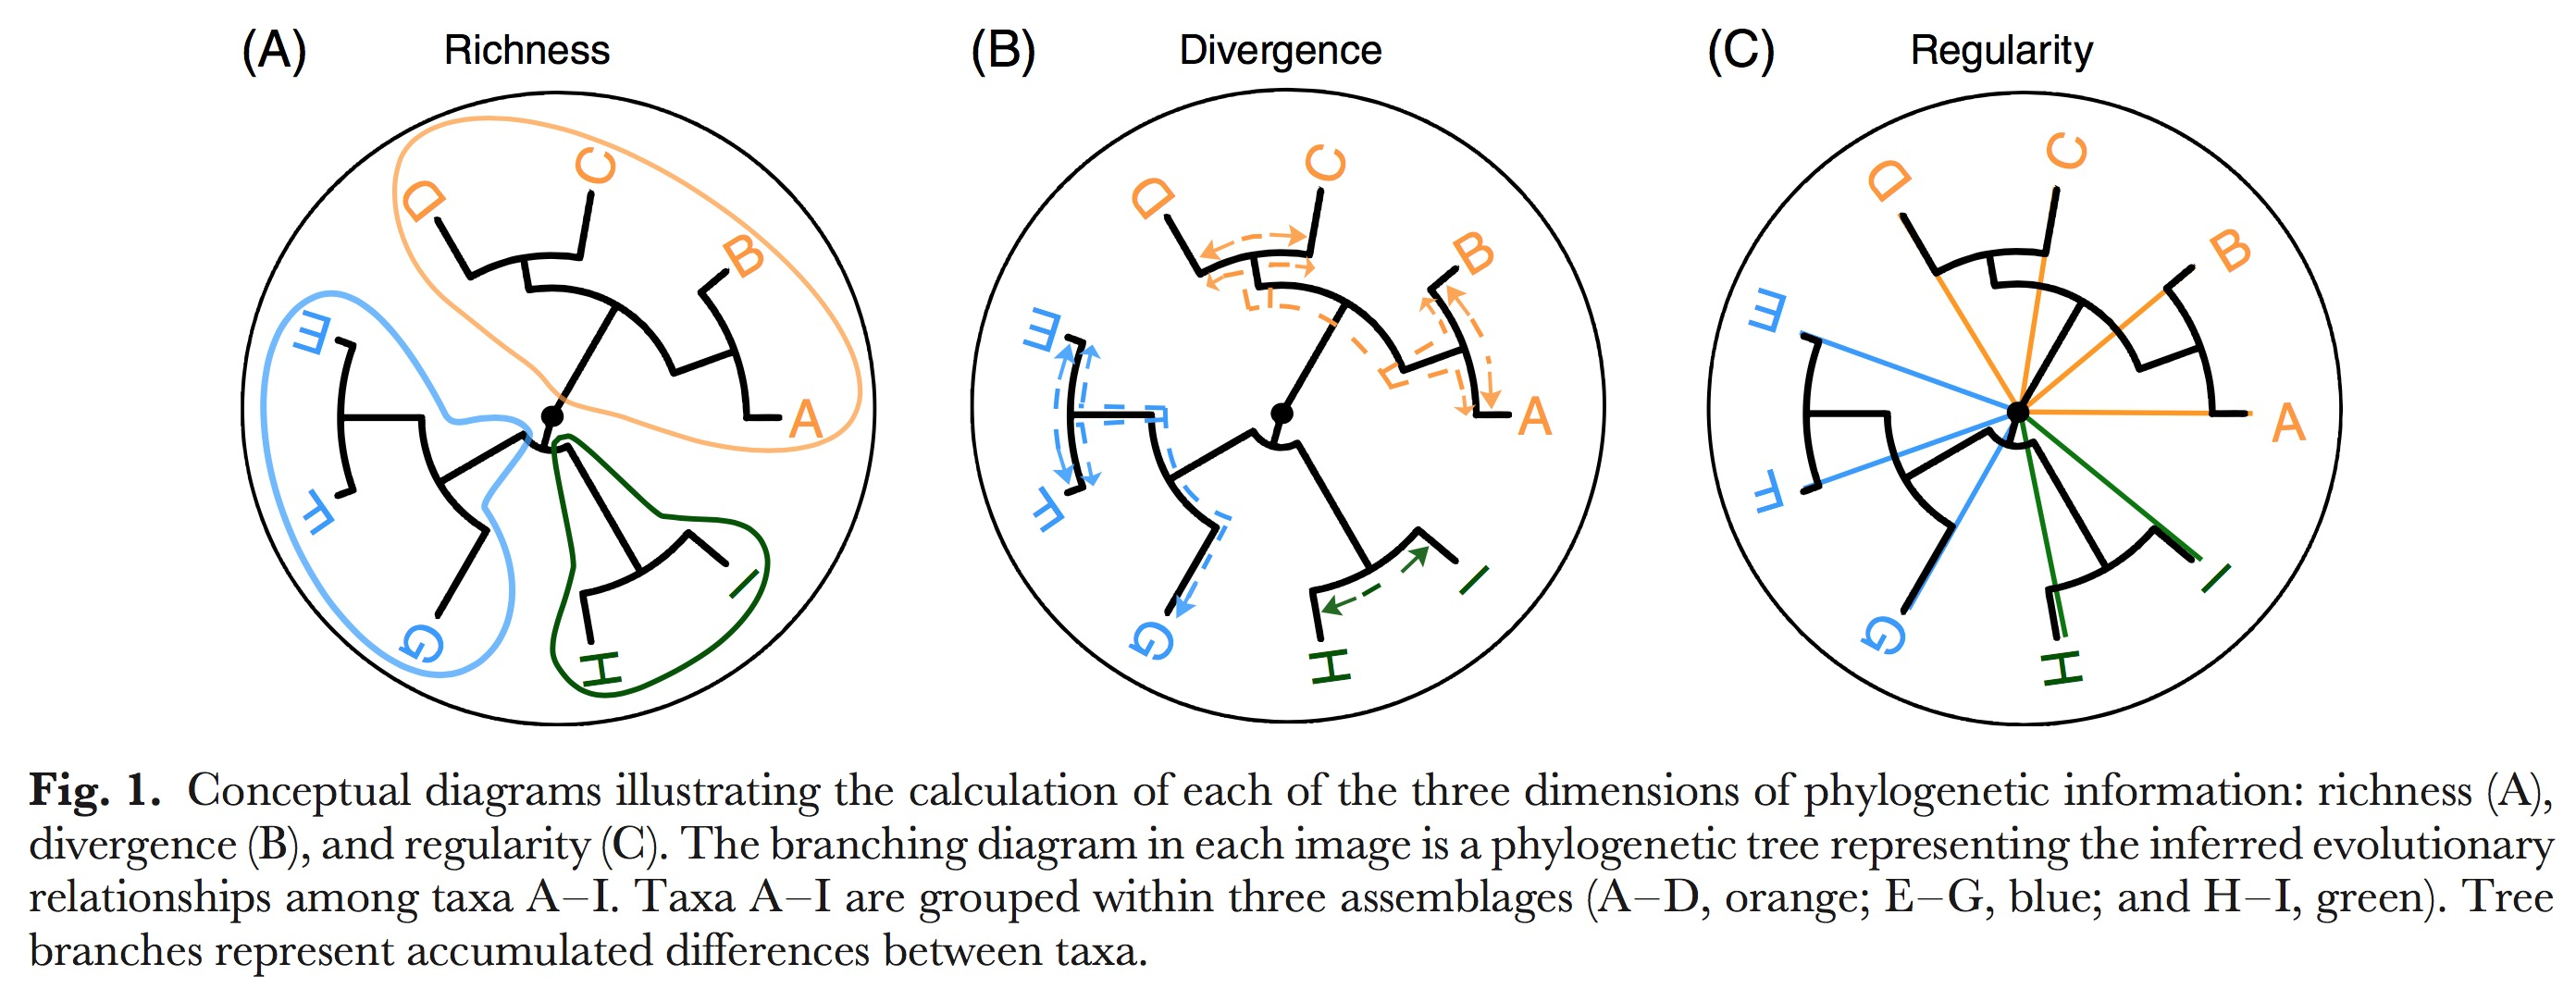
\includegraphics{Images/Tucker_2016/tree_concept.jpg}
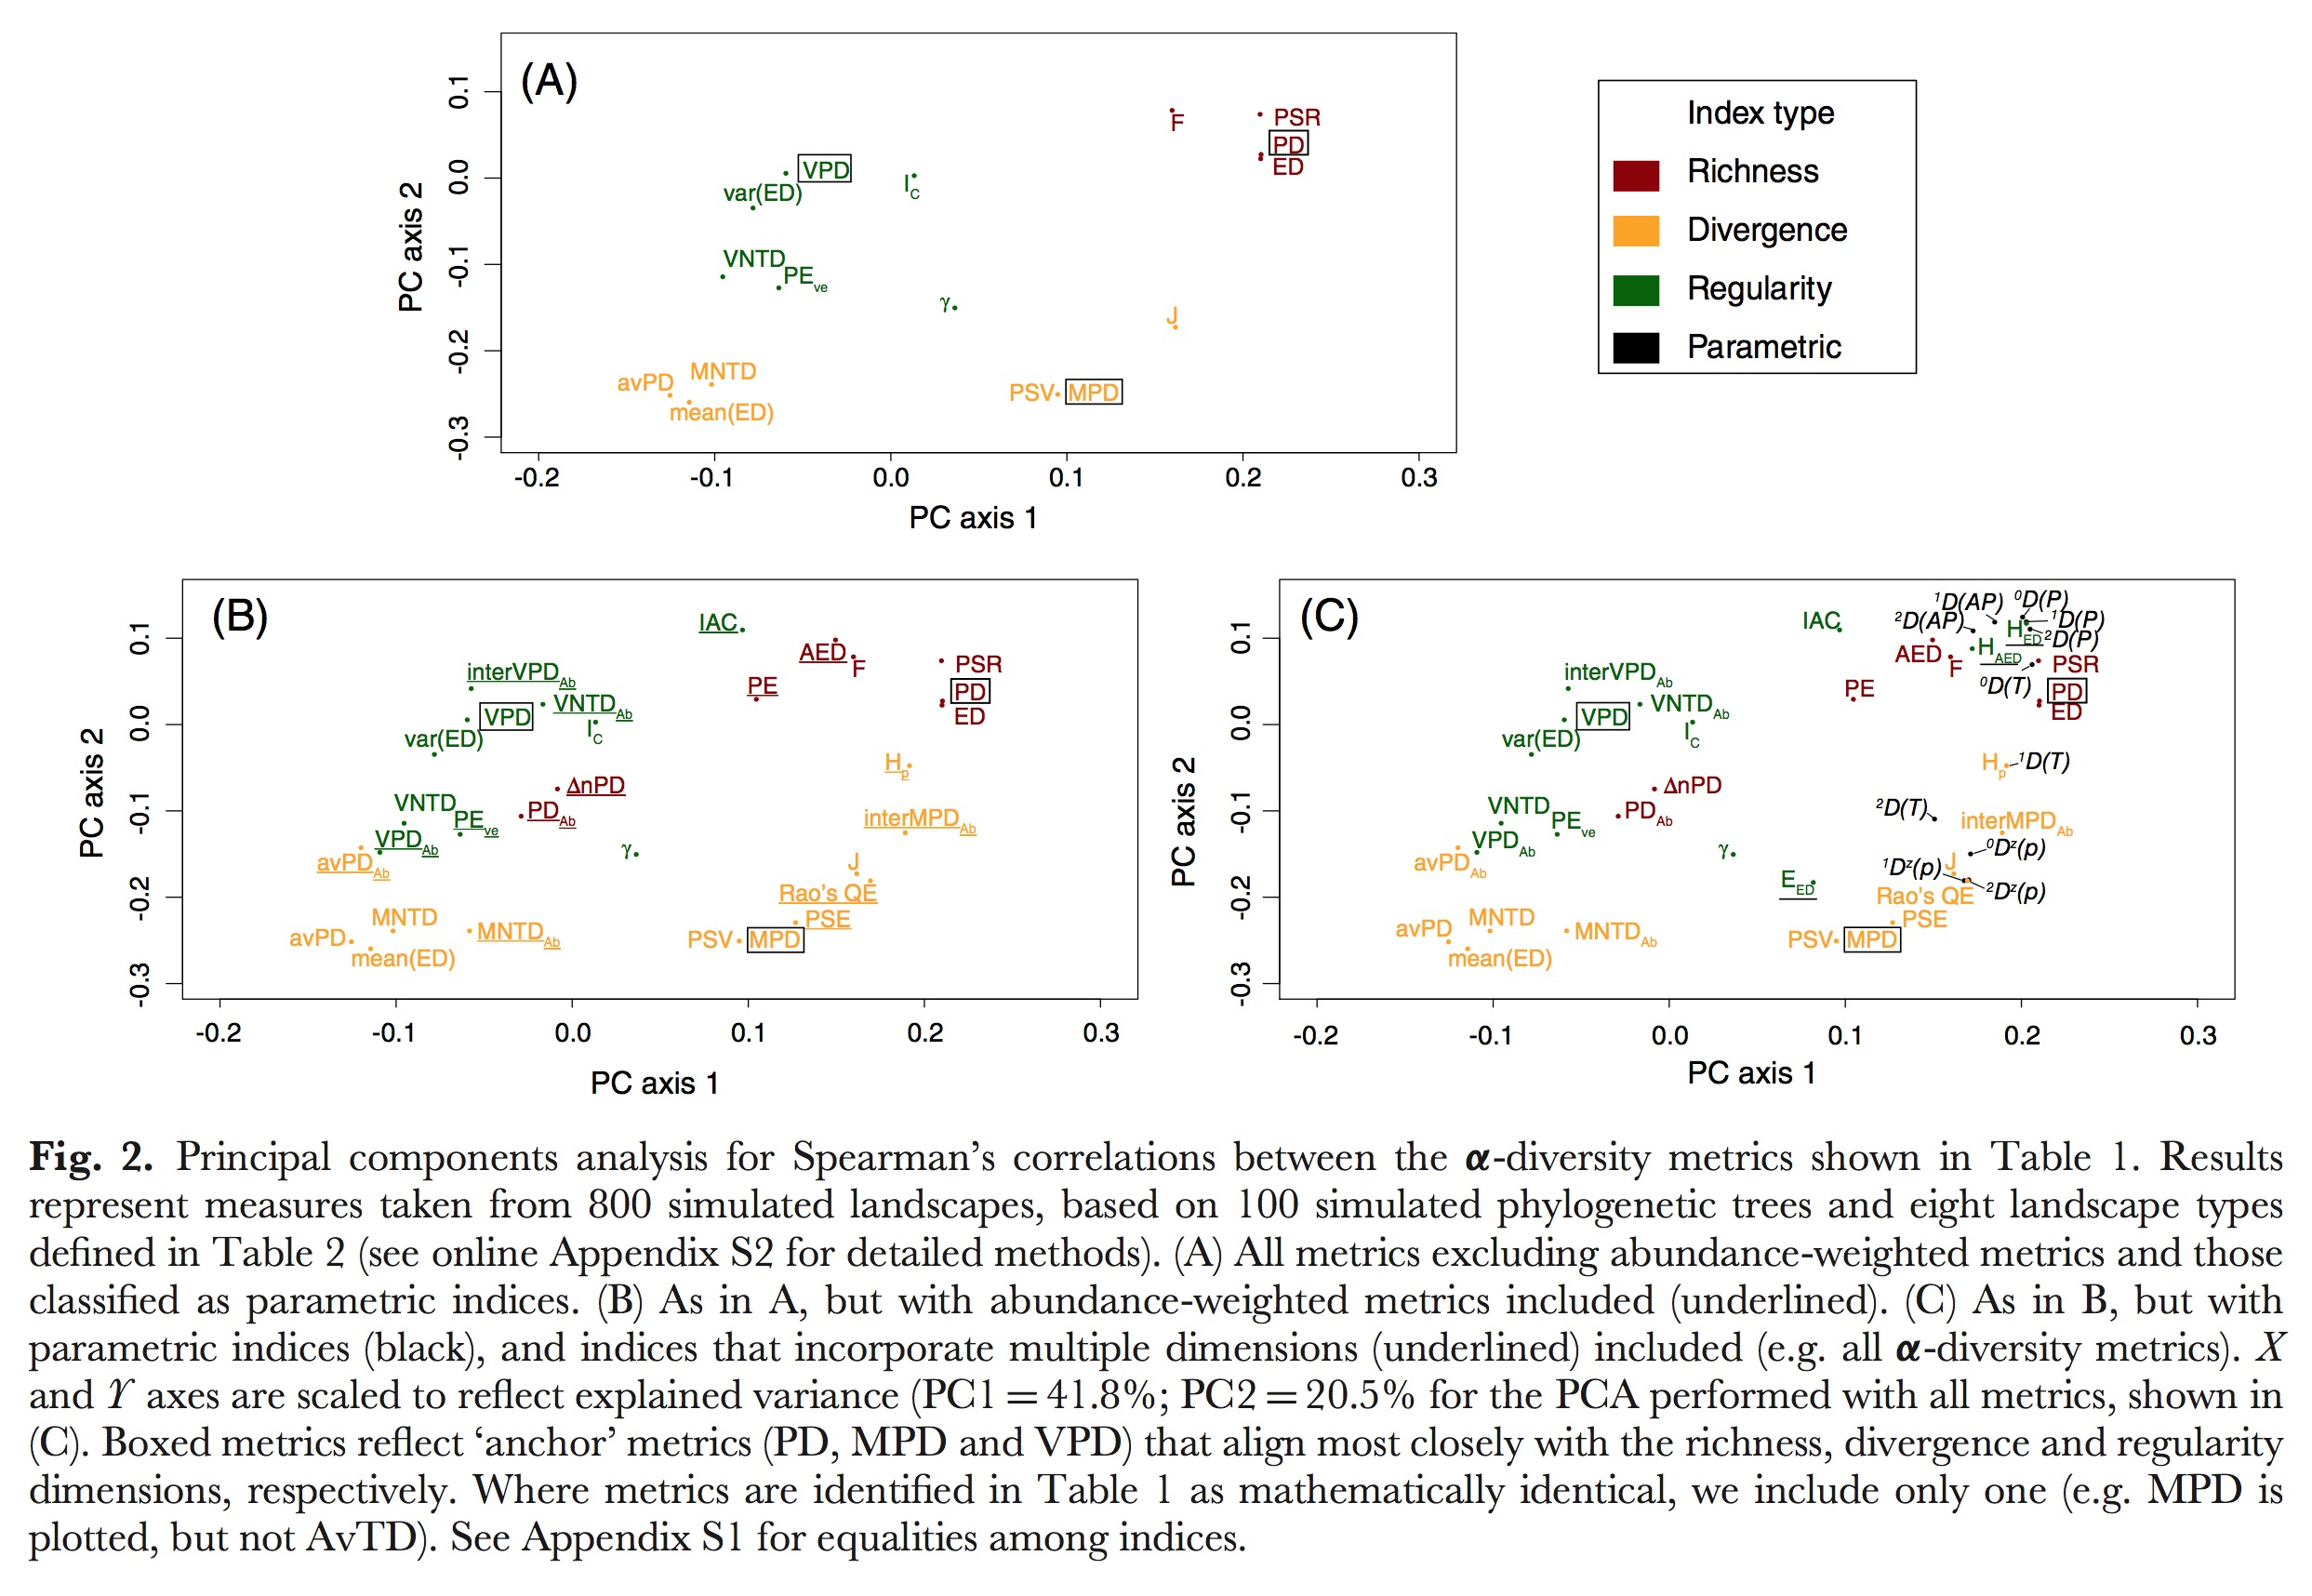
\includegraphics{Images/Tucker_2016/alpha_PCA.jpg}

\begin{figure}
\centering
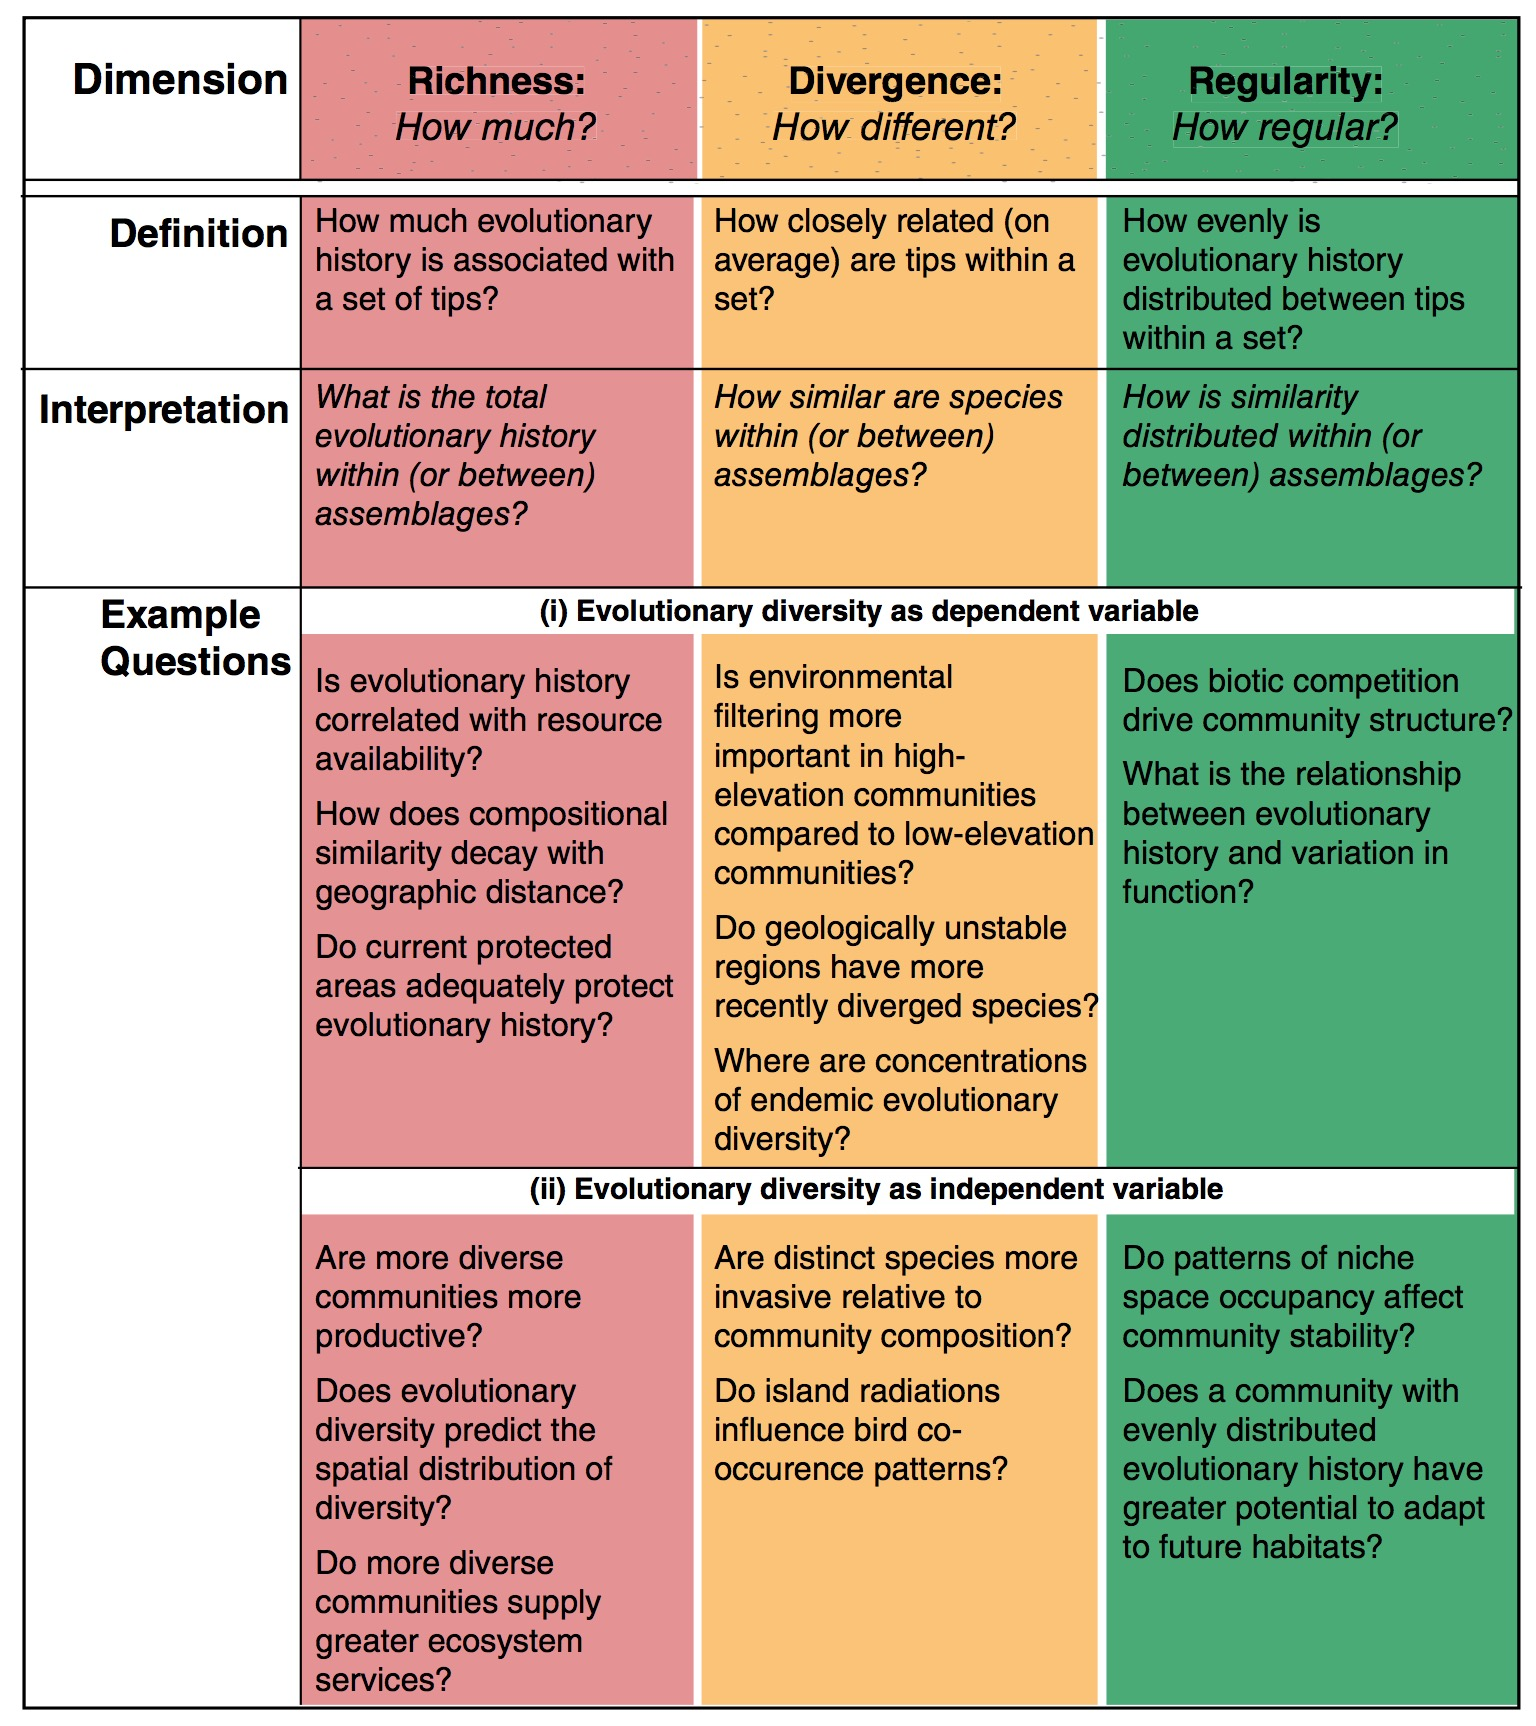
\includegraphics{Images/Tucker_2016/Three_type_summary.jpg}
\caption{From \citet{Tucker2016}}
\end{figure}

\begin{figure}
\centering
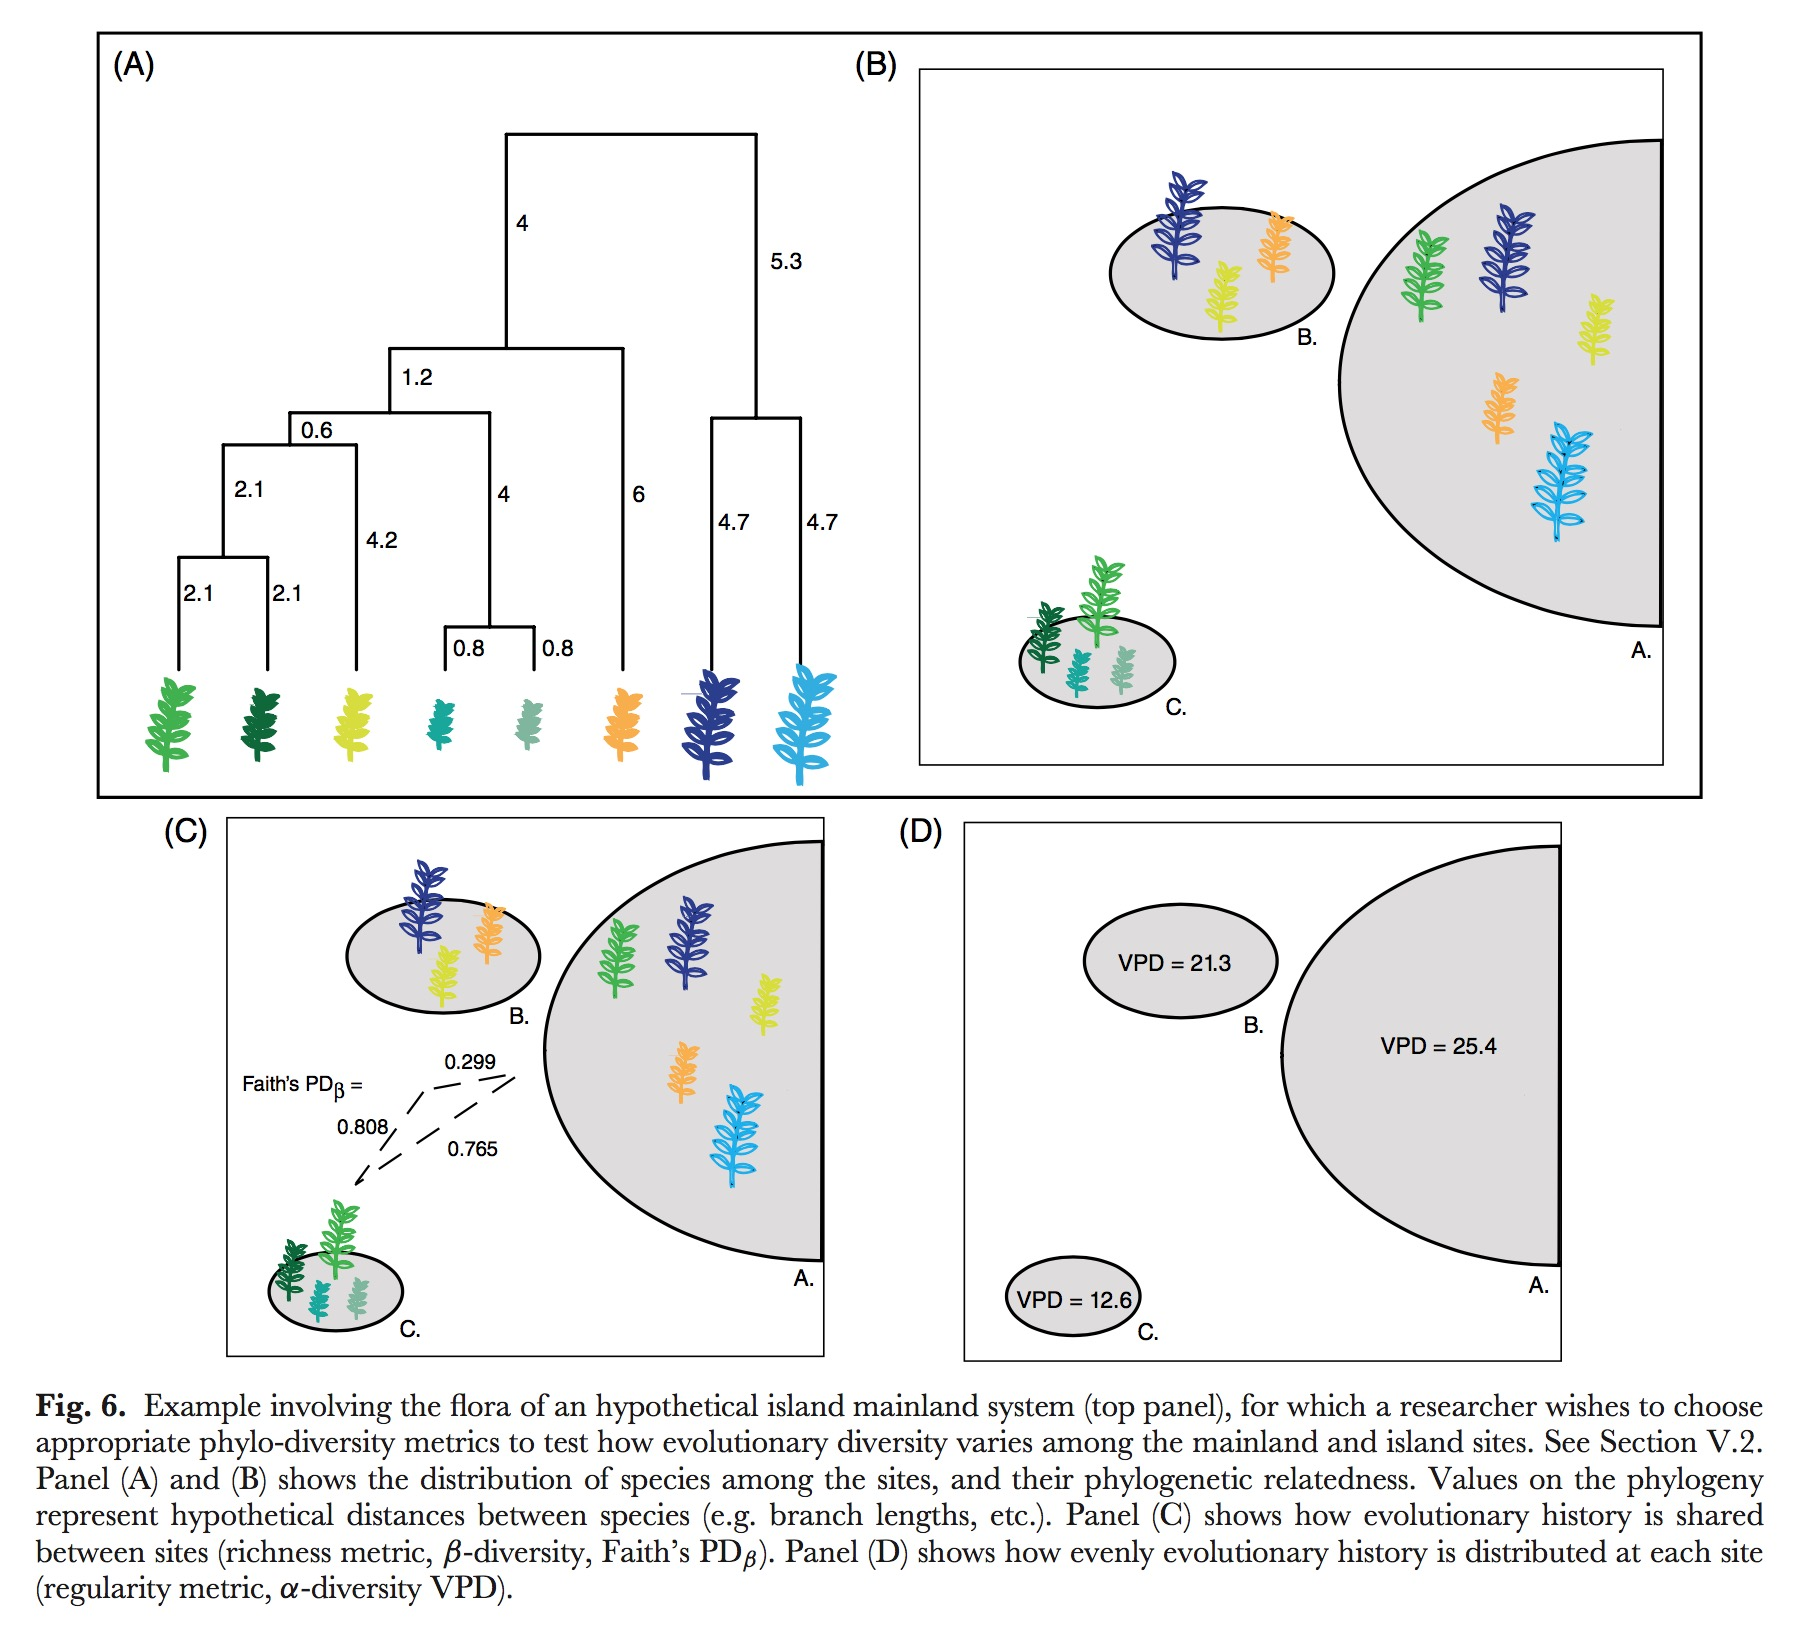
\includegraphics{Images/Tucker_2016/tutorial.jpg}
\caption{From \citet{Tucker2016}}
\end{figure}

\begin{Shaded}
\begin{Highlighting}[]
\KeywordTok{library}\NormalTok{(knitr)}
\KeywordTok{library}\NormalTok{(phytools)}
\KeywordTok{library}\NormalTok{(FARM)}
\KeywordTok{library}\NormalTok{(ROCR)}
\KeywordTok{library}\NormalTok{(spdep)}
\end{Highlighting}
\end{Shaded}

\begin{Shaded}
\begin{Highlighting}[]
\KeywordTok{load}\NormalTok{(}\StringTok{'~/Downloads/download.Rdata'}\NormalTok{)}

\NormalTok{this_tree <-}\StringTok{ }\NormalTok{myOut}\OperatorTok{$}\NormalTok{mytree}
\NormalTok{this_world <-}\StringTok{ }\NormalTok{myOut}\OperatorTok{$}\NormalTok{myWorld}
\end{Highlighting}
\end{Shaded}

\begin{Shaded}
\begin{Highlighting}[]
\KeywordTok{str}\NormalTok{(this_world)}
\end{Highlighting}
\end{Shaded}

\begin{verbatim}
## 'data.frame':    1253 obs. of  8 variables:
##  $ cellID     : num  1 2 3 4 5 6 7 8 9 10 ...
##  $ Longitude  : num  -60 12 28 -124 -63 ...
##  $ Latitude   : num  -25 10 -29 54 4 ...
##  $ Parent     : num  828 NA 216 616 901 NA NA NA NA NA ...
##  $ BirthT     : num  37.8 NA 37.6 31 36.2 ...
##  $ Trait      : num  1 NA 1 1 1 NA NA NA NA NA ...
##  $ Environment: num  2 2 2 1 2 1 2 1 1 1 ...
##  $ TipLabel   : chr  "t1" "t2" "t3" "t4" ...
\end{verbatim}

\begin{Shaded}
\begin{Highlighting}[]
\KeywordTok{str}\NormalTok{(this_tree)}
\end{Highlighting}
\end{Shaded}

\begin{verbatim}
## List of 4
##  $ edge       : num [1:910, 1:2] 457 460 463 560 892 892 560 463 466 466 ...
##  $ tip.label  : chr [1:456] "t862" "t409" "t260" "t204" ...
##  $ edge.length: num [1:910] 2.667 4.433 20.973 10.011 0.916 ...
##  $ Nnode      : num 455
##  - attr(*, "class")= chr "phylo"
##  - attr(*, "order")= chr "cladewise"
\end{verbatim}

\hypertarget{alpha-diversity-metrics}{\subsection{Alpha diversity
metrics}\label{alpha-diversity-metrics}}

\hypertarget{branch-lengths}{\subsubsection{Branch
Lengths}\label{branch-lengths}}

Branch length data is embedded in the tree object provided to this
function. The first step in summarizing the lengths is to extract those
data from the tree object. These data are called `edges' in the tree
object. We extract branch lengths and create an object called
`Branch\_lengths' for passing on to the other summary functions. The
histogram below shows the frequency of different branch lengths found
throughout the tree.

\begin{Shaded}
\begin{Highlighting}[]
\NormalTok{Branch_Lengths <-}\StringTok{ }\NormalTok{this_tree}\OperatorTok{$}\NormalTok{edge.length}
\end{Highlighting}
\end{Shaded}

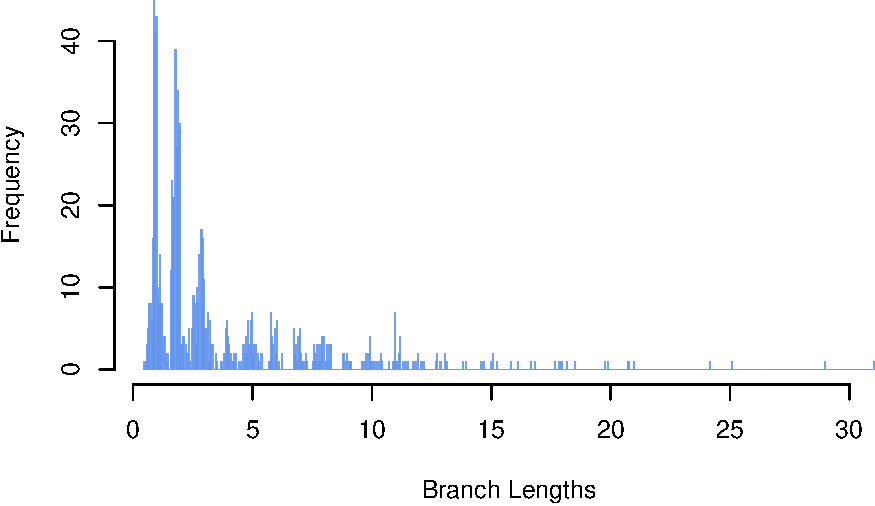
\includegraphics{bookdown-demo_files/figure-latex/unnamed-chunk-19-1.pdf}
We can summarize branch lengths according to normal summary statistics,
but it can be difficult to assign evolutionary meaning to some of these
metrics and so they are not regularly used as best I can tell. This lack
of meaning does not mean that these statistics couldn't be used to
distinguish between large simulated trees.

\begin{Shaded}
\begin{Highlighting}[]
\NormalTok{mean_branch_length <-}\StringTok{ }\KeywordTok{mean}\NormalTok{(Branch_Lengths)}
\NormalTok{variance_branch_length <-}\StringTok{ }\KeywordTok{var}\NormalTok{(Branch_Lengths)}
\NormalTok{SD_branch_length <-}\StringTok{ }\KeywordTok{sd}\NormalTok{(Branch_Lengths)}
\end{Highlighting}
\end{Shaded}

\begin{verbatim}
## [1] "mean branch length =  3.64753764473253"
\end{verbatim}

\begin{verbatim}
## [1] "variance in branch lengths =  14.9947769344804"
\end{verbatim}

\begin{verbatim}
## [1] "standard deviation in branch lengths =  3.87230899263998"
\end{verbatim}

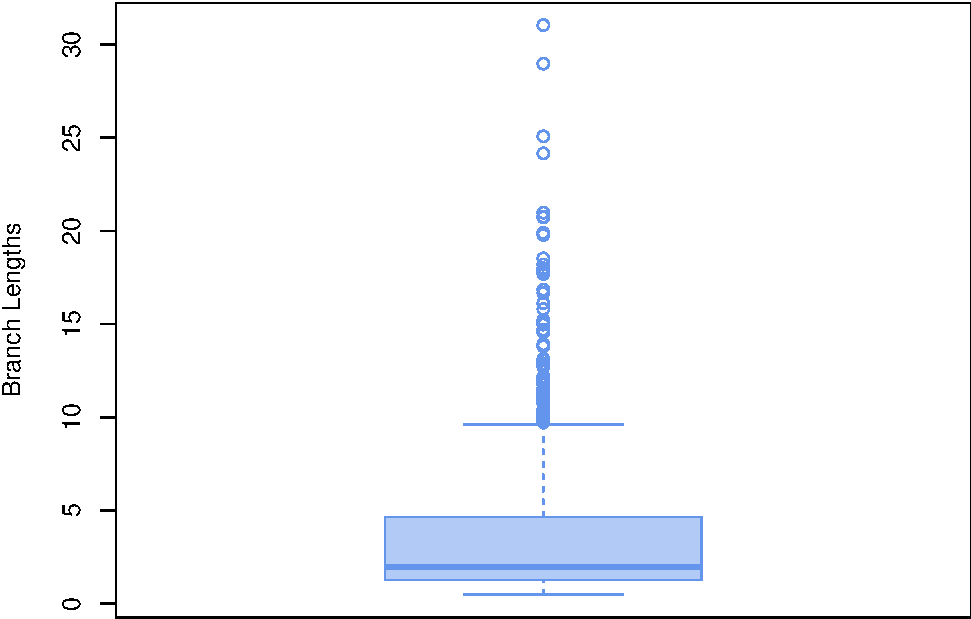
\includegraphics{bookdown-demo_files/figure-latex/unnamed-chunk-22-1.pdf}

\subsubsection{\texorpdfstring{Phylogenetic diversity
(\(PD\))}{Phylogenetic diversity (PD)}}\label{phylogenetic-diversity-pd}

Phylogenetic diversity (\(PD\)) is the summation (\(\sum\)) of all
branch lengths connecting species together, where \(B_{t}\) is the set
of included tips and \(L_{b}\) is Branch lengths \citep{Faith1992}. This
is an anchor test, which means it is regularly used, well understood,
and we should use it to anchor our work to past work. PD is a richness
measure, it tells us how much evolutionary history is associated with a
set of tips.

\[PD = \sum_{b \in B_{t}}^{}L_{b}\]

\begin{Shaded}
\begin{Highlighting}[]
\CommentTok{# Anchor test = PD (Faith's phylogenetic diversity)}
\NormalTok{Pylo_diversity_is_sum_of_BL <-}\StringTok{ }\KeywordTok{sum}\NormalTok{(Branch_Lengths)}
\NormalTok{Pylo_diversity_is_sum_of_BL}
\end{Highlighting}
\end{Shaded}

\begin{verbatim}
## [1] 3319.259
\end{verbatim}

There are variations on this measure that we have NOT implemented here.
It is popular to scale this measure according to some ecological driver.
\citet{Barker2002} scales branch lengths (\(L_{b}\)) by multiplying them
against the abundance of individuals at at tip (\(A_{b}\)). Others
\citep{Rosauer2009}, scale them by their range size instead (\(R_{b}\)).

\[\Delta n PD = \sum_{b \in B_{t}}^{}A_{b}L_{b}\]
\[PE = \sum_{b \in B_{t}}^{}\dfrac{L_{b}}{R_{b}}\] Argueing that
proportional abundance phylogenetic diversity (\(PD_{Ab}\)) is more
effective than the standard PD calculated from raw abundance,
\citet{Vellend2011} penned a new version of PD where \(B\) is the total
number of branch lengths (\(L_{b}\)). Note: We don't have abundance data
right now for the human project so this metric is not currently very
helpful.\\
\[PD_{Ab} = B * \dfrac{\sum_{b \in B_{t}}^{}A_{b}L_{b}}{\sum_{b \in B_{t}}^{}A_{b}}\]

\begin{Shaded}
\begin{Highlighting}[]
\CommentTok{#Calculate B}
\NormalTok{number_of_branches <-}\StringTok{ }\KeywordTok{length}\NormalTok{(Branch_Lengths)}
\NormalTok{number_of_branches}
\end{Highlighting}
\end{Shaded}

\begin{verbatim}
## [1] 910
\end{verbatim}

\subsubsection{\texorpdfstring{Average phylogenetic diversity
(\(avPD\))}{Average phylogenetic diversity (avPD)}}\label{average-phylogenetic-diversity-avpd}

Average phylogenetic diversity (\(avPD\)) \citep{Clarke2001} is a branch
length-based divergence indices where PD is divided by the total number
of tips (\(S\)) in the tree. \[avPD = \dfrac{PD}{S}\]

\begin{Shaded}
\begin{Highlighting}[]
\NormalTok{Number_of_tips <-}\StringTok{ }\KeywordTok{length}\NormalTok{(this_tree}\OperatorTok{$}\NormalTok{tip.label)}
\NormalTok{average_phylogenetic_diversity <-}\StringTok{ }\NormalTok{Pylo_diversity_is_sum_of_BL }\OperatorTok{/}\StringTok{ }\NormalTok{Number_of_tips}
\NormalTok{average_phylogenetic_diversity}
\end{Highlighting}
\end{Shaded}

\begin{verbatim}
## [1] 7.279077
\end{verbatim}

There is also a proportional abundance version of average phylogenetic
diversity (\(avPD_{Ab}\)) \citep{Tucker2016}. Again, we don't have
abundance values yet for D-place.
\[avPD_{Ab} = \dfrac{B * \dfrac{\sum_{b \in B_{t}}^{}A_{b}L_{b}}{\sum_{b \in B_{t}}^{}A_{b}}}{S}\]

\hypertarget{pairwise-distance-between-tips}{\subsection{Pairwise
distance between tips}\label{pairwise-distance-between-tips}}

This is the patristic distance, the sum of the branch lengths following
the shortest distance between two tips in a tree, implemented as a
distance matrix where every tip is compared to every other tip. This
distance function can be anything. We use euclidean and environmental
distance matrices heavily in the spatial analyses.

\subsubsection{Calculate the patristic distance between two taxa, for
all
taxa}\label{calculate-the-patristic-distance-between-two-taxa-for-all-taxa}

Calculate the patristic distance between two taxa using the R package
`phytools', this function takes a `phylo' tree object and returns a
distance matrix between tips. Need original citation.

\begin{Shaded}
\begin{Highlighting}[]
\NormalTok{## Pairwise distance between tips - From library(ape) in library(phytools)}
\NormalTok{Pairwise_dist <-}\StringTok{ }\KeywordTok{cophenetic}\NormalTok{(this_tree)}
\end{Highlighting}
\end{Shaded}

yields a distance matrix (list of 2D matrices) of all distances between
taxa.

\begin{verbatim}
##  num [1:456, 1:456] 0 57.9 78 57.9 72.7 ...
##  - attr(*, "dimnames")=List of 2
##   ..$ : chr [1:456] "t862" "t409" "t260" "t204" ...
##   ..$ : chr [1:456] "t862" "t409" "t260" "t204" ...
\end{verbatim}

\subsubsection{\texorpdfstring{Sum of all pairwise distances
(\(F\))}{Sum of all pairwise distances (F)}}\label{sum-of-all-pairwise-distances-f}

Now we can use a set of summary statistics to describe those pairwise
distances. The sum of all pairwise distances, \(F\), is formally called
`Extensive quadratic entropy'. \citep{Izsak2000}. Just as it was with
branch lengths, this is a richness measure and, accordingly, should be
used to answer richness questions.

\[F = \sum_{i} \sum_{j} d_{ij}\]

\begin{Shaded}
\begin{Highlighting}[]
\CommentTok{# F -- Extensive quadratic entropy}
\NormalTok{F_quadratic_entropy_is_sum_of_PD <-}\StringTok{ }\KeywordTok{sum}\NormalTok{(Pairwise_dist)}
\NormalTok{F_quadratic_entropy_is_sum_of_PD}
\end{Highlighting}
\end{Shaded}

\begin{verbatim}
## [1] 14047351
\end{verbatim}

\subsubsection{Mean pairwise distance
(MPD)}\label{mean-pairwise-distance-mpd}

Mean inter-species distances. The mean of all pairwise distances,
\(MPD\) (a.k.a. \(AvTD\), and \(\Delta^{+}\)), is the mean distance
between species. \citep{Clarke1998, Webb2002, Webb2008, Kembel2010}.
\[MPD = \dfrac{\sum_{ij} d_{ij}}{S(S-1)}\]

\begin{Shaded}
\begin{Highlighting}[]
\CommentTok{# Anchor test = MPD (mean pairwise distance)}
\NormalTok{Mean_pairwise_distance <-}\StringTok{ }
\StringTok{  }\NormalTok{Pairwise_dist }\OperatorTok{/}\StringTok{ }\NormalTok{(Number_of_tips }\OperatorTok{*}\StringTok{ }\NormalTok{(Number_of_tips }\OperatorTok{-}\StringTok{ }\DecValTok{1}\NormalTok{) ) }
\end{Highlighting}
\end{Shaded}

\begin{verbatim}
##  num [1:456, 1:456] 0 0.000279 0.000376 0.000279 0.00035 ...
##  - attr(*, "dimnames")=List of 2
##   ..$ : chr [1:456] "t862" "t409" "t260" "t204" ...
##   ..$ : chr [1:456] "t862" "t409" "t260" "t204" ...
\end{verbatim}

\subsubsection{MPD anchored to the root}\label{mpd-anchored-to-the-root}

There is an extention to mean pairwise distance calculations from
\citet{Helmus2010} called \(PSV\), \(PSR\), and \(PSE\), phylogenetic
species variability, phylogenetic species richness, and phylogenetic
species evenness. These measures take the basic pairwise distance
calculations and anchor them to the root of the tree so distances have a
common denominator. This extention is implemented by using the same
equations, just with a constrained set of \(d_{ij}\) conditions.
Specifically,

\[PSV = MPD = \dfrac{\sum_{ij} d_{ij}}{S(S-1)}\]
\[PSR = \sum_{i} {(\dfrac{1}{S-1} \sum_{j} {d_{ij}})}\]
\[PSE = \dfrac{S}{S-1} \sum_{ij} d_{ij}p_{i}p_{j}\]

with these specific values of \(d_{ij}\)

\[
d_{ji}=0.5*(c_{ii} + c_{jj} - c_{ij}) \\ 
\ \\
or \\
\ \\
d_{ij} = 1 - c_{ij} / (\sqrt{c_{ii}c_{jj}}) 
\] and \[
c_{ii} = the \ sum \ of \ branch \ lengths \ from \ tip \ i  \ to \ the \ root \ of \ the \ phylogenetic \ tree. \\
\ \\
c_{ij} = the \ sum \  of \ branch \ lengths \ from \ first \ common \ ancestor \ for \ i \ and \ j \ to \ the \ root.
\]

\subsubsection{Average distance between two randomly chosen
species}\label{average-distance-between-two-randomly-chosen-species}

\(J\), Intensive quadratic entropy, which is the average distance
between two randomly chosen species \citep{Izsak2000}
\[J = \dfrac{\sum_{ij}d_{ij}}{S^2} \]

\subsubsection{Simpson's diversity index for pairwise
distance}\label{simpsons-diversity-index-for-pairwise-distance}

There has been a long effort to pen a phylogenetic analogy to a
Simpson's diversity index.
\citep{Rao1982, Clarke1998, Pavoine2005, Hardy2007, Webb2002, Webb2008, Kembel2010}.
The conclusion seems to be that this measure is equivilent to scaling
\(MPD\) by abundance \(p_{i}\) and \(p_{j}\) to get \(MPD_{Ab}\). This
is also a special case of Rao's Quadratic Entropy, \(Roe's QE\). Note:
not using abundance measures yet for D-place data.

\[MPD_{Ab} = \sum_{i} \sum_{j} d_{ij} p_{i} p_{j}\]

\subsubsection{Interspecific comparisons of pairwise
distances}\label{interspecific-comparisons-of-pairwise-distances}

The interspecific variant (rather than the intraspecific default
described above) defines the expected phylogenetic distance between two
indivdiuals randomely drawn conditionally on the fact that they
indivdulas from different species.
\[InterMPD_{Ab} = \dfrac{\sum_{i} \sum_{j \ne i} d_{ij} p_{i} p_{j} }{\sum_{i} \sum_{j \ne i} d_{ij} p_{i} p_{j}}  \]

\subsubsection{\texorpdfstring{Variance in pairwise distances
(\(VPD\))}{Variance in pairwise distances (VPD)}}\label{variance-in-pairwise-distances-vpd}

Variance in pairwise distances, \(VPD\) (a.k.a. \(VarTD\) and
\(\Lambda^+\)), is a regularity indices. \citet{Clarke2001} Variance is
relative to tips, \(S\), not to total branches (\(B\) from above). These
are the residuals, they compare each individual pairwise connection to
the overall mean.

\[VPD = \dfrac{1}{S(S-1)} (\sum_{i} \sum_{j \ne i} {(d_{ij} - MPD)^2})\]

\begin{Shaded}
\begin{Highlighting}[]
\CommentTok{#need to adjust to equation above!}

\CommentTok{#Pairwise distance/all distances -- Variance of pairwise distances}

\CommentTok{# Anchor test = VPD (variation of pairwise distance)  }

\NormalTok{variance_pairwise_distance <-}\StringTok{ }\KeywordTok{var}\NormalTok{(}\KeywordTok{as.vector}\NormalTok{(Pairwise_dist))}
\end{Highlighting}
\end{Shaded}

Variants of \(VPD\) are \(VPD_{ab}\) and \(InterPVD_{Ab}\), where
variance is scaled by abundance or compared in and out of species. These
are also regularity indices.

\[
VPD_{Ab}= 
(\sum_{i} \sum_{j} n_{i} n_{j}) *
\dfrac{\sum_{i} \sum_{j} n_{i} n_{j} (d_{ij} - MPD_{Ab})^2}
{(\sum_{i} \sum_{j} n_{i} n_{j})^2 - \sum_{i} \sum_{j} (n_{i} n_{j})^2}
\\
or
\\
InterVPD_{Ab} = 
(\sum_{i} \sum_{j \ne i} n_{i} n_{j}) *
\dfrac{\sum_{i} \sum_{j \ne i} n_{i} n_{j} (d_{ij} - InterMPD_{Ab})^2}
{(\sum_{i} \sum_{j \ne i} n_{i} n_{j})^2 - \sum_{i} \sum_{j \ne i} (n_{i} n_{j})^2}
\]

\hypertarget{nearest-phylogenetic-neighbor}{\subsection{Nearest
phylogenetic neighbor}\label{nearest-phylogenetic-neighbor}}

\subsubsection{Divergence indices}\label{divergence-indices}

Divergence indices using nearest distance: \(MNTD\) and \(MNTD_{Ab}\),
Mean nearest taxon distance and Abundance-weighted MNTD
\citep{Webb2002, Webb2008, Kembel2010}.

\(MNTD\), mean nearest taxon distance, is the mean shortest distance
from a species to all other in the assemblage
\citep{Webb2002, Webb2008, Kembel2010}.\\
\[
MNTD = 
\dfrac{1}{S}
\sum_{i}
d_{i_{min}}
\]

\(MNTD_{AB}\), abundance adjusted mean nearest taxon distance. Adjusted
by species proportions (i.e.~species' relative abundances)
\citep{Webb2002, Webb2008, Kembel2010}\\
\[
MNTD_{Ab} = 
\sum_{i=1}^{S}
[d_{i_{min}} * p_{i}]
\]

\subsubsection{Regularity indices}\label{regularity-indices}

Regularity indices using nearest distances: \(VNTD\), \(VNTD_{Ab}\),
\(PE_{ev}\).

\(VNTD\), Variance in nearest taxon distances, is the variance in
nearest pairwise distance \citep{Tucker2016}. \[
VNTD = \dfrac{1}{S}
\sum_{i-1}^{S}
[(d_{i_{min}} - MNTD)^2]
\] \(VNTD_{Ab}\), Abundance weighted variance in nearest taxon
distances, is scales by abundance in the same way as descried above
\citep{Tucker2016}. \[
VNTD_{Ab} = \dfrac
{(\sum_{i} n_{i}) \sum_{i} n_{i} (d_{i_{min}} - MNTD_{Ab})^2}
{(\sum_{i} n_{i})^2 - \sum_{i} n_{i} ^2}
\]

\subsubsection{\texorpdfstring{Phylogenetic version of the funtional
\(FE_{ve}\)
index}{Phylogenetic version of the funtional FE\_\{ve\} index}}\label{phylogenetic-version-of-the-funtional-fe_ve-index}

\(PE_{ve}\), phylogenetic evenness is a phylogenetic version of the
funtional \(FE_{ve}\) index. First a minimum spanning tree (\(MST\)) is
computed using the cophenetic distance obtained from the phylogenetic
tree. The \(MST\) contains \(S-1\) Branches connection the \(S\)
species. We denote \(l\) a branch on the \(MST\), \(dist(i,j)\) is the
length the branch \(l\) that connects species \(i\) and \(j\). \(n_{i}\)
is, as defined above, the abundance of species \(i\) in the asseblage
\citep{Villeger2008, Dehling2014}.

\[
Weighted \ evenness: \\
EW_{i} = \dfrac{dist(i,j)}
{(n_{i} + n_{j})/(\sum_{k=1}^{S}n_{k})} \\
\ \\
Partial \ weighted \ evenness: \\ 
PEW_{l} = \dfrac
{EW_{l}}
{\sum_{l=1}^{S-1} EW_{l}} \\
\ \\
Phylogenetic \ evenness: \\
PE_{ve} = \dfrac
{\sum_{l=1}^{S-1} min(PEW_{l}, \dfrac{1}{S-1}) - (\dfrac{1}{S-1})}
{1- (\dfrac{1}{S-1})}
\]

\hypertarget{phylogenetic-isolation}{\subsection{Phylogenetic
isolation}\label{phylogenetic-isolation}}

A phylogenetic isolation index represents the relative isolation of a
given species within a phylogenetic tree. Several indices have been
proposed so far but we focus here on the evolutionary distinctiveness
index called `Fair Proportion' as proposed by \citet{Redding2003} and
\citet{Isaac2007}.

\subsubsection{Evolutionary distinctiveness (richness
indices)}\label{evolutionary-distinctiveness-richness-indices}

\(ED\), evolutionary distinctiveness is a richness indices. NOTE: not
equal to Faith's PD because the \(ED_{i}\) are computed from the
regional pool of species and sumed across a given assemblage (i.e.~a
subset of the regional species pool)
\citep{Tucker2016, Safi2013a, Redding2003, Isaac2007}.

\[
  ED = \sum_{i}ED_{i} \\
  \ \\ 
  where \ ED_{i} = \sum_{b \in B_{t_{i}}} \dfrac{L_{b}}{S_{b}} 
\]

\(AED\), Abundance-weighted \(ED\) \citep{Tucker2016, Cadotte2010}. \[
\sum_{i} AED_{i} \\
\ \\
where \ AED_{i} = \sum_{b \in B_{t_{i}}} \dfrac{L_{b}}{A_{b} }* p_{i}
\]

\begin{Shaded}
\begin{Highlighting}[]
\CommentTok{# Bruno's function for ED. Provided in library(FARM)}

\NormalTok{evol.distinct2 <-}\StringTok{ }\ControlFlowTok{function}\NormalTok{ (tree, }\DataTypeTok{type =} \KeywordTok{c}\NormalTok{(}\StringTok{"equal.splits"}\NormalTok{, }\StringTok{"fair.proportion"}\NormalTok{), }
    \DataTypeTok{scale =} \OtherTok{FALSE}\NormalTok{, }\DataTypeTok{use.branch.lengths =} \OtherTok{TRUE}\NormalTok{) }
\NormalTok{\{}
\NormalTok{    type <-}\StringTok{ }\KeywordTok{match.arg}\NormalTok{(type)}
    \ControlFlowTok{if}\NormalTok{ (}\KeywordTok{is.rooted}\NormalTok{(tree) }\OperatorTok{==}\StringTok{ }\OtherTok{FALSE}\NormalTok{) }
        \KeywordTok{warning}\NormalTok{(}\StringTok{"A rooted phylogeny is required for meaningful output of this function"}\NormalTok{, }
            \DataTypeTok{call. =} \OtherTok{FALSE}\NormalTok{)}
    \ControlFlowTok{if}\NormalTok{ (scale }\OperatorTok{==}\StringTok{ }\OtherTok{TRUE}\NormalTok{) \{}
        \ControlFlowTok{if}\NormalTok{ (}\KeywordTok{is.ultrametric}\NormalTok{(tree) }\OperatorTok{==}\StringTok{ }\OtherTok{TRUE}\NormalTok{) }
\NormalTok{            tree}\OperatorTok{$}\NormalTok{edge.length <-}\StringTok{ }\NormalTok{tree}\OperatorTok{$}\NormalTok{edge.length}\OperatorTok{/}\NormalTok{(}\KeywordTok{as.numeric}\NormalTok{(}\KeywordTok{branching.times}\NormalTok{(tree)[}\DecValTok{1}\NormalTok{]))}
        \ControlFlowTok{else}\NormalTok{ tree}\OperatorTok{$}\NormalTok{edge.length <-}\StringTok{ }\NormalTok{tree}\OperatorTok{$}\NormalTok{edge.length}\OperatorTok{/}\KeywordTok{sum}\NormalTok{(tree}\OperatorTok{$}\NormalTok{edge.length)}
\NormalTok{    \}}
    \ControlFlowTok{if}\NormalTok{ (use.branch.lengths }\OperatorTok{==}\StringTok{ }\OtherTok{FALSE}\NormalTok{) }
\NormalTok{        tree}\OperatorTok{$}\NormalTok{edge.length <-}\StringTok{ }\KeywordTok{rep}\NormalTok{(}\DecValTok{1}\NormalTok{, }\KeywordTok{length}\NormalTok{(tree}\OperatorTok{$}\NormalTok{edge.length))}
    \ControlFlowTok{for}\NormalTok{ (i }\ControlFlowTok{in} \DecValTok{1}\OperatorTok{:}\KeywordTok{length}\NormalTok{(tree}\OperatorTok{$}\NormalTok{tip.label)) \{}
\NormalTok{        spp <-}\StringTok{ }\NormalTok{tree}\OperatorTok{$}\NormalTok{tip.label[i]}
\NormalTok{        nodes <-}\StringTok{ }\KeywordTok{.get.nodes}\NormalTok{(tree, spp)}
\NormalTok{        nodes <-}\StringTok{ }\NormalTok{nodes[}\DecValTok{1}\OperatorTok{:}\NormalTok{(}\KeywordTok{length}\NormalTok{(nodes) }\OperatorTok{-}\StringTok{ }\DecValTok{1}\NormalTok{)]}
\NormalTok{        internal.brlen <-}\StringTok{ }\NormalTok{tree}\OperatorTok{$}\NormalTok{edge.length[}\KeywordTok{which}\NormalTok{(tree}\OperatorTok{$}\NormalTok{edge[, }
            \DecValTok{2}\NormalTok{] }\OperatorTok\StringTok{ }\NormalTok{nodes)]}
        \ControlFlowTok{if}\NormalTok{ (}\KeywordTok{length}\NormalTok{(internal.brlen) }\OperatorTok{!=}\StringTok{ }\DecValTok{0}\NormalTok{) \{}
\NormalTok{            internal.brlen <-}\StringTok{ }\NormalTok{internal.brlen }\OperatorTok{*}\StringTok{ }\ControlFlowTok{switch}\NormalTok{(type, }\DataTypeTok{equal.splits =} \KeywordTok{sort}\NormalTok{(}\KeywordTok{rep}\NormalTok{(}\FloatTok{0.5}\NormalTok{, }
                \KeywordTok{length}\NormalTok{(internal.brlen))}\OperatorTok{^}\KeywordTok{c}\NormalTok{(}\DecValTok{1}\OperatorTok{:}\KeywordTok{length}\NormalTok{(internal.brlen))), }
                \DataTypeTok{fair.proportion =}\NormalTok{ \{}
                  \ControlFlowTok{for}\NormalTok{ (j }\ControlFlowTok{in} \DecValTok{1}\OperatorTok{:}\KeywordTok{length}\NormalTok{(nodes)) \{}
\NormalTok{                    sons <-}\StringTok{ }\KeywordTok{.node.desc}\NormalTok{(tree, nodes[j])}
\NormalTok{                    n.descendents <-}\StringTok{ }\KeywordTok{length}\NormalTok{(sons}\OperatorTok{$}\NormalTok{tips)}
                    \ControlFlowTok{if}\NormalTok{ (j }\OperatorTok{==}\StringTok{ }\DecValTok{1}\NormalTok{) portion <-}\StringTok{ }\NormalTok{n.descendents }\ControlFlowTok{else}\NormalTok{ portion <-}\StringTok{ }\KeywordTok{c}\NormalTok{(n.descendents, }
\NormalTok{                      portion)}
\NormalTok{                  \}}
                  \DecValTok{1}\OperatorTok{/}\NormalTok{portion}
\NormalTok{                \})}
\NormalTok{        \}}
\NormalTok{        ED <-}\StringTok{ }\KeywordTok{sum}\NormalTok{(internal.brlen, tree}\OperatorTok{$}\NormalTok{edge.length[}\KeywordTok{which.edge}\NormalTok{(tree, }
\NormalTok{            spp)])}
        \ControlFlowTok{if}\NormalTok{ (i }\OperatorTok{==}\StringTok{ }\DecValTok{1}\NormalTok{) }
\NormalTok{            w <-}\StringTok{ }\NormalTok{ED}
        \ControlFlowTok{else}\NormalTok{ w <-}\StringTok{ }\KeywordTok{c}\NormalTok{(w, ED)}
\NormalTok{    \}}
    \KeywordTok{return}\NormalTok{(w)}
\NormalTok{\}}
\end{Highlighting}
\end{Shaded}

Evolutionary distinctiveness is our basic measure of phylogenetic
isolation. \#This should likely be `fair proportions' instead of
`equal.splits'.

\begin{Shaded}
\begin{Highlighting}[]
\CommentTok{# Calculate ED}
\CommentTok{# Using equal.splits method, faster computation}
\CommentTok{# Evolutionary_distinctiveness_i <- evol.distinct2(this_tree, type = "equal.splits")  }

\CommentTok{# ED - Summed evolutionary distinctiveness}
\CommentTok{# Evolutionary_distinctiveness_sum <- sum(Evolutionary_distinctiveness_i)}
\end{Highlighting}
\end{Shaded}

\begin{Shaded}
\begin{Highlighting}[]
\CommentTok{#Evolutionary_distinctiveness_sum}
\end{Highlighting}
\end{Shaded}

We can run some standard summary statistics (mean and variance) on this
ED measure. var(Ed) shows up close to VPD on the PCAs in the intro
\citep{Tucker2016}.

\begin{Shaded}
\begin{Highlighting}[]
\CommentTok{# mean(ED)}
\CommentTok{# mean_Phylogenetic_isolation <- mean(Evolutionary_distinctiveness_i)}

\CommentTok{# var(ED)}
\CommentTok{#variance_Phylogenetic_isolation <- var(Evolutionary_distinctiveness_i)}
\end{Highlighting}
\end{Shaded}

\begin{Shaded}
\begin{Highlighting}[]
\CommentTok{#mean_Phylogenetic_isolation}
\CommentTok{#variance_Phylogenetic_isolation}
\end{Highlighting}
\end{Shaded}

\subsubsection{Mean evolutionary distinctiveness (divergence
indices)}\label{mean-evolutionary-distinctiveness-divergence-indices}

The divergence indices version for \(ED\) is mean evolutionary
distinctiveness, \(MED\). The mean of evolutionary distinctiveness
\citep{Redding2003, Isaac2007}. \[
MED = \dfrac
{\sum_{i} ED_{i}}
{S} \\
\ \\
with \\
\ \\
ED_{i} = \sum_{b \in B_{t_{i}}} \dfrac{L_{b}}{S_{b}}
\] \#\#\#\# Entropy measure of evolutonary distinctiveness (regularity
indices) The regularity indices for \(ED\)/phylogenetic isolation are
\(H_{ED}\), \(E_{ED}\), \(var(ED)\), \(H_{AED}\)

\(H_{ED}\), Entropy measure of evolutionary distinctiveness, is the
shannon index applied to evolutionary distinctiveness values
\citep{Cadotte2010}. \[
H_{ED} = -\sum_{i=1}^{S}
((\dfrac{ED_{i}}{\sum_{i=1}^{S} ED_{i}})
* \ln (\dfrac{ED_{i}}{\sum_{i=1}^{S} ED_{i}}))
\]

\(E_{ED}\), Equitability of evolutionary distinctiveness, is \(H_{ED}\)
controlled for species richness \citep{Cadotte2010}.

\[
E_{ED} = \dfrac{H_{ED}}{\ln(S)}
\] \(var(ED)\), Variance in evolutinoary distinctiveness, is the
variance of species evolutionary distinctiveness \citep{Tucker2016}.

\[
var(ED) = \dfrac{1}{S-1} *
\sum_{i=1}^{S}
(ED_{i}-\dfrac{\sum_{i=1}^{S} ED_{i}}{S})^2
\] \(H_{ED_{Ab}}\), Abundance-weighted version of \(H_{ED}\)
\citep{Cadotte2010}.

\[
H_{ED_{Ab}} = -\sum_{i=1}^{S}
(\dfrac{n_{i}AED_{i}}{\sum_{i=1}^{S} n_{i}AED_{i}} *
\ln(\dfrac{n_{i}AED_{i}}{\sum_{i=1}^{S} n_{i}AED_{i}}))
\]

\hypertarget{beta-diversity}{\section{Beta
diversity}\label{beta-diversity}}

We currently are not using any beta diversity metrics but there are many
to choose from if we decide to add them later.

\hypertarget{tree-topology}{\section{Tree
topology}\label{tree-topology}}

Tree topology is a measure of the shape of the overall tree. The tree
can be lopsided side-to-side or front-to-back.

Our most trusted index for the tippy vs trunky of a tree is the gamma
index, \(\gamma\).The index characterizes the distribution of branching
events within the tree. Trees with \(\gamma < 0\) have relatively longer
branches towards the tips of the phylogeny (tippy trees), whereas trees
with \(\gamma > 0\) have relatively longer inter-nodal distances towards
the root of the phylogeny (stemmy trees). tk represents an `evolutionary
period' (limits are given by two speciation events) or equivalently an
internode distance \citep{Pybus2000}.

\[
  \gamma = \dfrac
  {(\dfrac{1}{S-2}* \sum_{i=2}^{S-1} (\sum_{k=2}^{i} Kt_{k}))- \dfrac{1}{2} * \sum_{j=2}^{S} jt_{j}}
  {(\sum_{j=2}^{S} jt_{j}) * \sqrt{\dfrac{1}{12*(S-2)}}}
\]

\begin{Shaded}
\begin{Highlighting}[]
\CommentTok{# ltt function from library(phytools)}
\NormalTok{ltt <-}\StringTok{ }\ControlFlowTok{function}\NormalTok{ (tree, }\DataTypeTok{plot =} \OtherTok{TRUE}\NormalTok{, }\DataTypeTok{drop.extinct =} \OtherTok{FALSE}\NormalTok{, }\DataTypeTok{log.lineages =} \OtherTok{TRUE}\NormalTok{, }
    \DataTypeTok{gamma =} \OtherTok{TRUE}\NormalTok{, ...) }
\NormalTok{\{}
\NormalTok{    tol <-}\StringTok{ }\FloatTok{1e-06}
    \ControlFlowTok{if}\NormalTok{ (}\OperatorTok{!}\KeywordTok{inherits}\NormalTok{(tree, }\StringTok{"phylo"}\NormalTok{) }\OperatorTok{&&}\StringTok{ }\OperatorTok{!}\KeywordTok{inherits}\NormalTok{(tree, }\StringTok{"multiPhylo"}\NormalTok{)) }
        \KeywordTok{stop}\NormalTok{(}\StringTok{"tree must be object of class }\CharTok{\textbackslash{}"}\StringTok{phylo}\CharTok{\textbackslash{}"}\StringTok{ or }\CharTok{\textbackslash{}"}\StringTok{multiPhylo}\CharTok{\textbackslash{}"}\StringTok{."}\NormalTok{)}
    \ControlFlowTok{if}\NormalTok{ (}\KeywordTok{inherits}\NormalTok{(tree, }\StringTok{"multiPhylo"}\NormalTok{)) \{}
\NormalTok{        obj <-}\StringTok{ }\KeywordTok{lapply}\NormalTok{(tree, ltt, }\DataTypeTok{plot =} \OtherTok{FALSE}\NormalTok{, }\DataTypeTok{drop.extinct =}\NormalTok{ drop.extinct, }
            \DataTypeTok{log.lineages =}\NormalTok{ log.lineages, }\DataTypeTok{gamma =}\NormalTok{ gamma)}
        \KeywordTok{class}\NormalTok{(obj) <-}\StringTok{ "multiLtt"}
\NormalTok{    \}}
    \ControlFlowTok{else}\NormalTok{ \{}
\NormalTok{        tree <-}\StringTok{ }\KeywordTok{reorder.phylo}\NormalTok{(tree, }\DataTypeTok{order =} \StringTok{"cladewise"}\NormalTok{)}
        \ControlFlowTok{if}\NormalTok{ (}\OperatorTok{!}\KeywordTok{is.null}\NormalTok{(tree}\OperatorTok{$}\NormalTok{node.label)) \{}
\NormalTok{            node.names <-}\StringTok{ }\KeywordTok{setNames}\NormalTok{(tree}\OperatorTok{$}\NormalTok{node.label, }\DecValTok{1}\OperatorTok{:}\NormalTok{tree}\OperatorTok{$}\NormalTok{Nnode }\OperatorTok{+}\StringTok{ }
\StringTok{                }\KeywordTok{Ntip}\NormalTok{(tree))}
\NormalTok{            tree}\OperatorTok{$}\NormalTok{node.label <-}\StringTok{ }\OtherTok{NULL}
\NormalTok{        \}}
        \ControlFlowTok{else}\NormalTok{ node.names <-}\StringTok{ }\OtherTok{NULL}
        \ControlFlowTok{if}\NormalTok{ (}\KeywordTok{is.ultrametric}\NormalTok{(tree)) \{}
\NormalTok{            h <-}\StringTok{ }\KeywordTok{max}\NormalTok{(}\KeywordTok{nodeHeights}\NormalTok{(tree))}
\NormalTok{            time <-}\StringTok{ }\KeywordTok{c}\NormalTok{(}\DecValTok{0}\NormalTok{, h }\OperatorTok{-}\StringTok{ }\KeywordTok{sort}\NormalTok{(}\KeywordTok{branching.times}\NormalTok{(tree), }\DataTypeTok{decreasing =} \OtherTok{TRUE}\NormalTok{), }
\NormalTok{                h)}
\NormalTok{            nodes <-}\StringTok{ }\KeywordTok{as.numeric}\NormalTok{(}\KeywordTok{names}\NormalTok{(time)[}\DecValTok{2}\OperatorTok{:}\NormalTok{(}\KeywordTok{length}\NormalTok{(time) }\OperatorTok{-}\StringTok{ }
\StringTok{                }\DecValTok{1}\NormalTok{)])}
\NormalTok{            ltt <-}\StringTok{ }\KeywordTok{c}\NormalTok{(}\KeywordTok{cumsum}\NormalTok{(}\KeywordTok{c}\NormalTok{(}\DecValTok{1}\NormalTok{, }\KeywordTok{sapply}\NormalTok{(nodes, }\ControlFlowTok{function}\NormalTok{(x, y) }\KeywordTok{sum}\NormalTok{(y }\OperatorTok{==}\StringTok{ }
\StringTok{                }\NormalTok{x) }\OperatorTok{-}\StringTok{ }\DecValTok{1}\NormalTok{, }\DataTypeTok{y =}\NormalTok{ tree}\OperatorTok{$}\NormalTok{edge[, }\DecValTok{1}\NormalTok{]))), }\KeywordTok{length}\NormalTok{(tree}\OperatorTok{$}\NormalTok{tip.label))}
            \KeywordTok{names}\NormalTok{(ltt) <-}\StringTok{ }\KeywordTok{names}\NormalTok{(time)}
\NormalTok{        \}}
        \ControlFlowTok{else}\NormalTok{ \{}
\NormalTok{            drop.extinct.tips <-}\StringTok{ }\ControlFlowTok{function}\NormalTok{(phy) \{}
\NormalTok{                temp <-}\StringTok{ }\KeywordTok{diag}\NormalTok{(}\KeywordTok{vcv}\NormalTok{(phy))}
                \ControlFlowTok{if}\NormalTok{ (}\KeywordTok{length}\NormalTok{(temp[temp }\OperatorTok{<}\StringTok{ }\NormalTok{(}\KeywordTok{max}\NormalTok{(temp) }\OperatorTok{-}\StringTok{ }\NormalTok{tol)]) }\OperatorTok{>}\StringTok{ }
\StringTok{                  }\DecValTok{0}\NormalTok{) }
\NormalTok{                  pruned.phy <-}\StringTok{ }\KeywordTok{drop.tip}\NormalTok{(phy, }\KeywordTok{names}\NormalTok{(temp[temp }\OperatorTok{<}\StringTok{ }
\StringTok{                    }\NormalTok{(}\KeywordTok{max}\NormalTok{(temp) }\OperatorTok{-}\StringTok{ }\NormalTok{tol)]))}
                \ControlFlowTok{else}\NormalTok{ pruned.phy <-}\StringTok{ }\NormalTok{phy}
                \KeywordTok{return}\NormalTok{(pruned.phy)}
\NormalTok{            \}}
            \ControlFlowTok{if}\NormalTok{ (drop.extinct }\OperatorTok{==}\StringTok{ }\OtherTok{TRUE}\NormalTok{) }
\NormalTok{                tree <-}\StringTok{ }\KeywordTok{drop.extinct.tips}\NormalTok{(tree)}
\NormalTok{            root <-}\StringTok{ }\KeywordTok{length}\NormalTok{(tree}\OperatorTok{$}\NormalTok{tip) }\OperatorTok{+}\StringTok{ }\DecValTok{1}
\NormalTok{            node.height <-}\StringTok{ }\KeywordTok{matrix}\NormalTok{(}\OtherTok{NA}\NormalTok{, }\KeywordTok{nrow}\NormalTok{(tree}\OperatorTok{$}\NormalTok{edge), }\DecValTok{2}\NormalTok{)}
            \ControlFlowTok{for}\NormalTok{ (i }\ControlFlowTok{in} \DecValTok{1}\OperatorTok{:}\KeywordTok{nrow}\NormalTok{(tree}\OperatorTok{$}\NormalTok{edge)) \{}
                \ControlFlowTok{if}\NormalTok{ (tree}\OperatorTok{$}\NormalTok{edge[i, }\DecValTok{1}\NormalTok{] }\OperatorTok{==}\StringTok{ }\NormalTok{root) \{}
\NormalTok{                  node.height[i, }\DecValTok{1}\NormalTok{] <-}\StringTok{ }\DecValTok{0}
\NormalTok{                  node.height[i, }\DecValTok{2}\NormalTok{] <-}\StringTok{ }\NormalTok{tree}\OperatorTok{$}\NormalTok{edge.length[i]}
\NormalTok{                \}}
                \ControlFlowTok{else}\NormalTok{ \{}
\NormalTok{                  node.height[i, }\DecValTok{1}\NormalTok{] <-}\StringTok{ }\NormalTok{node.height[}\KeywordTok{match}\NormalTok{(tree}\OperatorTok{$}\NormalTok{edge[i, }
                    \DecValTok{1}\NormalTok{], tree}\OperatorTok{$}\NormalTok{edge[, }\DecValTok{2}\NormalTok{]), }\DecValTok{2}\NormalTok{]}
\NormalTok{                  node.height[i, }\DecValTok{2}\NormalTok{] <-}\StringTok{ }\NormalTok{node.height[i, }\DecValTok{1}\NormalTok{] }\OperatorTok{+}\StringTok{ }\NormalTok{tree}\OperatorTok{$}\NormalTok{edge.length[i]}
\NormalTok{                \}}
\NormalTok{            \}}
\NormalTok{            ltt <-}\StringTok{ }\KeywordTok{vector}\NormalTok{()}
\NormalTok{            tree.length <-}\StringTok{ }\KeywordTok{max}\NormalTok{(node.height)}
\NormalTok{            n.extinct <-}\StringTok{ }\KeywordTok{sum}\NormalTok{(node.height[tree}\OperatorTok{$}\NormalTok{edge[, }\DecValTok{2}\NormalTok{] }\OperatorTok{<=}\StringTok{ }\KeywordTok{length}\NormalTok{(tree}\OperatorTok{$}\NormalTok{tip), }
                \DecValTok{2}\NormalTok{] }\OperatorTok{<}\StringTok{ }\NormalTok{(tree.length }\OperatorTok{-}\StringTok{ }\NormalTok{tol))}
\NormalTok{            node.height[tree}\OperatorTok{$}\NormalTok{edge[, }\DecValTok{2}\NormalTok{] }\OperatorTok{<=}\StringTok{ }\KeywordTok{length}\NormalTok{(tree}\OperatorTok{$}\NormalTok{tip), }\DecValTok{2}\NormalTok{] <-}\StringTok{ }\NormalTok{node.height[tree}\OperatorTok{$}\NormalTok{edge[, }
                \DecValTok{2}\NormalTok{] }\OperatorTok{<=}\StringTok{ }\KeywordTok{length}\NormalTok{(tree}\OperatorTok{$}\NormalTok{tip), }\DecValTok{2}\NormalTok{] }\OperatorTok{+}\StringTok{ }\FloatTok{1.1} \OperatorTok{*}\StringTok{ }\NormalTok{tol}
\NormalTok{            time <-}\StringTok{ }\KeywordTok{c}\NormalTok{(}\DecValTok{0}\NormalTok{, node.height[, }\DecValTok{2}\NormalTok{])}
            \KeywordTok{names}\NormalTok{(time) <-}\StringTok{ }\KeywordTok{as.character}\NormalTok{(}\KeywordTok{c}\NormalTok{(root, tree}\OperatorTok{$}\NormalTok{edge[, }\DecValTok{2}\NormalTok{]))}
\NormalTok{            temp <-}\StringTok{ }\KeywordTok{vector}\NormalTok{()}
\NormalTok{            time <-}\StringTok{ }\NormalTok{time[}\KeywordTok{order}\NormalTok{(time)]}
\NormalTok{            time <-}\StringTok{ }\NormalTok{time[}\DecValTok{1}\OperatorTok{:}\NormalTok{(tree}\OperatorTok{$}\NormalTok{Nnode }\OperatorTok{+}\StringTok{ }\NormalTok{n.extinct }\OperatorTok{+}\StringTok{ }\DecValTok{1}\NormalTok{)]}
            \ControlFlowTok{for}\NormalTok{ (i }\ControlFlowTok{in} \DecValTok{1}\OperatorTok{:}\NormalTok{(}\KeywordTok{length}\NormalTok{(time) }\OperatorTok{-}\StringTok{ }\DecValTok{1}\NormalTok{)) \{}
\NormalTok{                ltt[i] <-}\StringTok{ }\DecValTok{0}
                \ControlFlowTok{for}\NormalTok{ (j }\ControlFlowTok{in} \DecValTok{1}\OperatorTok{:}\KeywordTok{nrow}\NormalTok{(node.height)) ltt[i] <-}\StringTok{ }\NormalTok{ltt[i] }\OperatorTok{+}\StringTok{ }
\StringTok{                  }\NormalTok{(time[i] }\OperatorTok{>=}\StringTok{ }\NormalTok{(node.height[j, }\DecValTok{1}\NormalTok{] }\OperatorTok{-}\StringTok{ }\NormalTok{tol) }\OperatorTok{&&}\StringTok{ }\NormalTok{time[i] }\OperatorTok{<=}\StringTok{ }
\StringTok{                    }\NormalTok{(node.height[j, }\DecValTok{2}\NormalTok{] }\OperatorTok{-}\StringTok{ }\NormalTok{tol))}
\NormalTok{            \}}
\NormalTok{            ltt[i }\OperatorTok{+}\StringTok{ }\DecValTok{1}\NormalTok{] <-}\StringTok{ }\DecValTok{0}
            \ControlFlowTok{for}\NormalTok{ (j }\ControlFlowTok{in} \DecValTok{1}\OperatorTok{:}\KeywordTok{nrow}\NormalTok{(node.height)) ltt[i }\OperatorTok{+}\StringTok{ }\DecValTok{1}\NormalTok{] <-}\StringTok{ }\NormalTok{ltt[i }\OperatorTok{+}\StringTok{ }
\StringTok{                }\DecValTok{1}\NormalTok{] }\OperatorTok{+}\StringTok{ }\NormalTok{(time[i }\OperatorTok{+}\StringTok{ }\DecValTok{1}\NormalTok{] }\OperatorTok{<=}\StringTok{ }\NormalTok{(node.height[j, }\DecValTok{2}\NormalTok{] }\OperatorTok{+}\StringTok{ }\NormalTok{tol))}
            \KeywordTok{names}\NormalTok{(ltt) <-}\StringTok{ }\KeywordTok{names}\NormalTok{(time)}
\NormalTok{            ltt <-}\StringTok{ }\KeywordTok{c}\NormalTok{(}\DecValTok{1}\NormalTok{, ltt)}
\NormalTok{            time <-}\StringTok{ }\KeywordTok{c}\NormalTok{(}\DecValTok{0}\NormalTok{, time)}
\NormalTok{            time[}\KeywordTok{length}\NormalTok{(time)] <-}\StringTok{ }\NormalTok{time[}\KeywordTok{length}\NormalTok{(time)] }\OperatorTok{-}\StringTok{ }\FloatTok{1.1} \OperatorTok{*}\StringTok{ }
\StringTok{                }\NormalTok{tol}
\NormalTok{        \}}
        \ControlFlowTok{if}\NormalTok{ (}\OperatorTok{!}\KeywordTok{is.null}\NormalTok{(node.names)) \{}
\NormalTok{            nn <-}\StringTok{ }\KeywordTok{sapply}\NormalTok{(}\KeywordTok{names}\NormalTok{(time), }\ControlFlowTok{function}\NormalTok{(x, y) }\ControlFlowTok{if}\NormalTok{ (}\KeywordTok{any}\NormalTok{(}\KeywordTok{names}\NormalTok{(y) }\OperatorTok{==}\StringTok{ }
\StringTok{                }\NormalTok{x)) }
\NormalTok{                y[}\KeywordTok{which}\NormalTok{(}\KeywordTok{names}\NormalTok{(y) }\OperatorTok{==}\StringTok{ }\NormalTok{x)]}
            \ControlFlowTok{else} \StringTok{""}\NormalTok{, }\DataTypeTok{y =}\NormalTok{ node.names)}
            \KeywordTok{names}\NormalTok{(ltt) <-}\StringTok{ }\KeywordTok{names}\NormalTok{(time) <-}\StringTok{ }\NormalTok{nn}
\NormalTok{        \}}
        \ControlFlowTok{if}\NormalTok{ (gamma }\OperatorTok{==}\StringTok{ }\OtherTok{FALSE}\NormalTok{) \{}
\NormalTok{            obj <-}\StringTok{ }\KeywordTok{list}\NormalTok{(}\DataTypeTok{ltt =}\NormalTok{ ltt, }\DataTypeTok{times =}\NormalTok{ time, }\DataTypeTok{tree =}\NormalTok{ tree)}
            \KeywordTok{class}\NormalTok{(obj) <-}\StringTok{ "ltt"}
\NormalTok{        \}}
        \ControlFlowTok{else}\NormalTok{ \{}
\NormalTok{            gam <-}\StringTok{ }\KeywordTok{gammatest}\NormalTok{(}\KeywordTok{list}\NormalTok{(}\DataTypeTok{ltt =}\NormalTok{ ltt, }\DataTypeTok{times =}\NormalTok{ time))}
\NormalTok{            obj <-}\StringTok{ }\KeywordTok{list}\NormalTok{(}\DataTypeTok{ltt =}\NormalTok{ ltt, }\DataTypeTok{times =}\NormalTok{ time, }\DataTypeTok{gamma =}\NormalTok{ gam}\OperatorTok{$}\NormalTok{gamma, }
                \DataTypeTok{p =}\NormalTok{ gam}\OperatorTok{$}\NormalTok{p, }\DataTypeTok{tree =}\NormalTok{ tree)}
            \KeywordTok{class}\NormalTok{(obj) <-}\StringTok{ "ltt"}
\NormalTok{        \}}
\NormalTok{    \}}
    \ControlFlowTok{if}\NormalTok{ (plot) }
        \KeywordTok{plot}\NormalTok{(obj, }\DataTypeTok{log.lineages =}\NormalTok{ log.lineages, ...)}
\NormalTok{    obj}
\NormalTok{\}}
\OperatorTok{<}\NormalTok{environment}\OperatorTok{:}\StringTok{ }\NormalTok{namespace}\OperatorTok{:}\NormalTok{phytools}\OperatorTok{>}
\end{Highlighting}
\end{Shaded}

\begin{Shaded}
\begin{Highlighting}[]
\NormalTok{ltts <-}\StringTok{ }\KeywordTok{ltt}\NormalTok{(this_tree, }\DataTypeTok{gamma =} \OtherTok{TRUE}\NormalTok{, }\DataTypeTok{plot =} \OtherTok{FALSE}\NormalTok{)}
\NormalTok{ltts}
\end{Highlighting}
\end{Shaded}

\begin{verbatim}
## Object of class "ltt" containing:
## 
## (1) A phylogenetic tree with 456 tips and 455 internal nodes.
## 
## (2) Vectors containing the number of lineages (ltt) and branching times (times) on the tree.
## 
## (3) A value for Pybus & Harvey's "gamma" statistic of 1.7401, p-value = 0.0818.
\end{verbatim}

\begin{Shaded}
\begin{Highlighting}[]
\KeywordTok{str}\NormalTok{(ltts)}
\end{Highlighting}
\end{Shaded}

\begin{verbatim}
## List of 5
##  $ ltt  : Named num [1:457] 1 2 3 4 5 6 7 8 9 10 ...
##   ..- attr(*, "names")= chr [1:457] "" "457" "458" "459" ...
##  $ times: Named num [1:457] 0.00 2.84e-13 1.00 2.00 2.67 ...
##   ..- attr(*, "names")= chr [1:457] "" "457" "458" "459" ...
##  $ gamma: num 1.74
##  $ p    : num 0.0818
##  $ tree :List of 4
##   ..$ edge       : num [1:910, 1:2] 457 460 463 560 892 892 560 463 466 466 ...
##   ..$ tip.label  : chr [1:456] "t862" "t409" "t260" "t204" ...
##   ..$ edge.length: num [1:910] 2.667 4.433 20.973 10.011 0.916 ...
##   ..$ Nnode      : num 455
##   ..- attr(*, "class")= chr "phylo"
##   ..- attr(*, "order")= chr "cladewise"
##  - attr(*, "class")= chr "ltt"
\end{verbatim}

\begin{Shaded}
\begin{Highlighting}[]
\NormalTok{lineages_through_time <-}\StringTok{ }\KeywordTok{as.numeric}\NormalTok{(ltts[[}\DecValTok{1}\NormalTok{]])}
\NormalTok{time_steps <-}\StringTok{ }\KeywordTok{as.numeric}\NormalTok{(ltts[[}\DecValTok{2}\NormalTok{]])}
\CommentTok{#extract Gamma index}
\NormalTok{gamma <-}\StringTok{ }\NormalTok{ltts[[}\DecValTok{3}\NormalTok{]]}
\NormalTok{gamma_p_value <-}\StringTok{ }\NormalTok{ltts[[}\DecValTok{4}\NormalTok{]]}
\end{Highlighting}
\end{Shaded}

\begin{Shaded}
\begin{Highlighting}[]
\NormalTok{lineages_through_time }
\end{Highlighting}
\end{Shaded}

\begin{verbatim}
##   [1]   1   2   3   4   5   6   7   8   9  10  11  12  13  14  15  16  17
##  [18]  18  19  20  21  22  23  24  25  26  27  28  29  30  31  32  33  34
##  [35]  35  36  37  38  39  40  41  42  43  44  45  46  47  48  49  50  51
##  [52]  52  53  54  55  56  57  58  59  60  61  62  63  64  65  66  67  68
##  [69]  69  70  71  72  73  74  75  76  77  78  79  80  81  82  83  84  85
##  [86]  86  87  88  89  90  91  92  93  94  95  96  97  98  99 100 101 102
## [103] 103 104 105 106 107 108 109 110 111 112 113 114 115 116 117 118 119
## [120] 120 121 122 123 124 125 126 127 128 129 130 131 132 133 134 135 136
## [137] 137 138 139 140 141 142 143 144 145 146 147 148 149 150 151 152 153
## [154] 154 155 156 157 158 159 160 161 162 163 164 165 166 167 168 169 170
## [171] 171 172 173 174 175 176 177 178 179 180 181 182 183 184 185 186 187
## [188] 188 189 190 191 192 193 194 195 196 197 198 199 200 201 202 203 204
## [205] 205 206 207 208 209 210 211 212 213 214 215 216 217 218 219 220 221
## [222] 222 223 224 225 226 227 228 229 230 231 232 233 234 235 236 237 238
## [239] 239 240 241 242 243 244 245 246 247 248 249 250 251 252 253 254 255
## [256] 256 257 258 259 260 261 262 263 264 265 266 267 268 269 270 271 272
## [273] 273 274 275 276 277 278 279 280 281 282 283 284 285 286 287 288 289
## [290] 290 291 292 293 294 295 296 297 298 299 300 301 302 303 304 305 306
## [307] 307 308 309 310 311 312 313 314 315 316 317 318 319 320 321 322 323
## [324] 324 325 326 327 328 329 330 331 332 333 334 335 336 337 338 339 340
## [341] 341 342 343 344 345 346 347 348 349 350 351 352 353 354 355 356 357
## [358] 358 359 360 361 362 363 364 365 366 367 368 369 370 371 372 373 374
## [375] 375 376 377 378 379 380 381 382 383 384 385 386 387 388 389 390 391
## [392] 392 393 394 395 396 397 398 399 400 401 402 403 404 405 406 407 408
## [409] 409 410 411 412 413 414 415 416 417 418 419 420 421 422 423 424 425
## [426] 426 427 428 429 430 431 432 433 434 435 436 437 438 439 440 441 442
## [443] 443 444 445 446 447 448 449 450 451 452 453 454 455 456 456
\end{verbatim}

\begin{Shaded}
\begin{Highlighting}[]
\NormalTok{time_steps }
\end{Highlighting}
\end{Shaded}

\begin{verbatim}
##   [1] 0.000000e+00 2.842171e-13 1.000000e+00 2.000000e+00 2.666667e+00
##   [6] 3.333333e+00 5.461538e+00 7.100000e+00 7.450000e+00 9.296296e+00
##  [11] 1.003030e+01 1.024242e+01 1.121429e+01 1.126190e+01 1.200000e+01
##  [16] 1.203509e+01 1.215789e+01 1.217544e+01 1.314815e+01 1.316667e+01
##  [21] 1.335185e+01 1.416667e+01 1.428788e+01 1.436364e+01 1.502222e+01
##  [26] 1.503333e+01 1.512222e+01 1.527778e+01 1.600000e+01 1.630588e+01
##  [31] 1.720588e+01 1.733333e+01 1.734314e+01 1.738235e+01 1.808036e+01
##  [36] 1.833036e+01 1.901613e+01 1.913710e+01 1.915323e+01 1.921774e+01
##  [41] 1.923387e+01 2.006504e+01 2.021138e+01 2.030081e+01 2.038211e+01
##  [46] 2.043902e+01 2.047154e+01 2.100000e+01 2.101361e+01 2.117687e+01
##  [51] 2.130612e+01 2.131973e+01 2.132653e+01 2.204065e+01 2.233333e+01
##  [56] 2.234146e+01 2.236585e+01 2.247967e+01 2.254472e+01 2.314872e+01
##  [61] 2.315897e+01 2.320513e+01 2.406011e+01 2.409290e+01 2.409836e+01
##  [66] 2.424044e+01 2.431694e+01 2.501579e+01 2.503158e+01 2.506842e+01
##  [71] 2.512105e+01 2.514737e+01 2.515263e+01 2.516842e+01 2.517895e+01
##  [76] 2.519474e+01 2.529474e+01 2.534737e+01 2.600985e+01 2.602956e+01
##  [81] 2.604433e+01 2.605419e+01 2.607882e+01 2.623153e+01 2.624138e+01
##  [86] 2.625123e+01 2.625616e+01 2.627586e+01 2.629064e+01 2.630049e+01
##  [91] 2.631034e+01 2.706135e+01 2.711043e+01 2.717791e+01 2.724540e+01
##  [96] 2.725153e+01 2.734356e+01 2.747239e+01 2.749693e+01 2.755828e+01
## [101] 2.757669e+01 2.800385e+01 2.802692e+01 2.804231e+01 2.807308e+01
## [106] 2.813077e+01 2.814615e+01 2.816154e+01 2.816923e+01 2.818462e+01
## [111] 2.820000e+01 2.821923e+01 2.825385e+01 2.830000e+01 2.901115e+01
## [116] 2.901487e+01 2.902230e+01 2.903346e+01 2.905204e+01 2.909294e+01
## [121] 2.912268e+01 2.915985e+01 2.923048e+01 2.938662e+01 3.000683e+01
## [126] 3.001365e+01 3.003413e+01 3.015358e+01 3.018771e+01 3.019795e+01
## [131] 3.021502e+01 3.022184e+01 3.028669e+01 3.032765e+01 3.101894e+01
## [136] 3.104545e+01 3.107955e+01 3.109848e+01 3.115152e+01 3.115909e+01
## [141] 3.117424e+01 3.118939e+01 3.120455e+01 3.120833e+01 3.122348e+01
## [146] 3.125000e+01 3.125758e+01 3.128030e+01 3.129924e+01 3.132197e+01
## [151] 3.138636e+01 3.140909e+01 3.141288e+01 3.141667e+01 3.142803e+01
## [156] 3.201587e+01 3.201905e+01 3.202222e+01 3.202540e+01 3.204127e+01
## [161] 3.205079e+01 3.206984e+01 3.209206e+01 3.210476e+01 3.215873e+01
## [166] 3.216825e+01 3.218095e+01 3.218730e+01 3.223810e+01 3.225714e+01
## [171] 3.228571e+01 3.233651e+01 3.302521e+01 3.303922e+01 3.305042e+01
## [176] 3.305602e+01 3.311204e+01 3.311765e+01 3.312885e+01 3.313445e+01
## [181] 3.314566e+01 3.314846e+01 3.315126e+01 3.315966e+01 3.318487e+01
## [186] 3.319328e+01 3.321289e+01 3.322129e+01 3.322409e+01 3.322689e+01
## [191] 3.322969e+01 3.323249e+01 3.323529e+01 3.323810e+01 3.327171e+01
## [196] 3.328852e+01 3.400290e+01 3.402899e+01 3.405217e+01 3.408406e+01
## [201] 3.409855e+01 3.410725e+01 3.412754e+01 3.413623e+01 3.415652e+01
## [206] 3.417101e+01 3.418261e+01 3.421449e+01 3.422609e+01 3.423478e+01
## [211] 3.425217e+01 3.425797e+01 3.427536e+01 3.427826e+01 3.428986e+01
## [216] 3.430145e+01 3.431304e+01 3.431884e+01 3.432464e+01 3.433043e+01
## [221] 3.435072e+01 3.435942e+01 3.436812e+01 3.500431e+01 3.503664e+01
## [226] 3.504310e+01 3.506897e+01 3.507112e+01 3.508190e+01 3.508836e+01
## [231] 3.509698e+01 3.509914e+01 3.510129e+01 3.510991e+01 3.511853e+01
## [236] 3.600000e+01 3.600651e+01 3.601303e+01 3.602280e+01 3.603257e+01
## [241] 3.603583e+01 3.606189e+01 3.606515e+01 3.606840e+01 3.607166e+01
## [246] 3.607492e+01 3.608143e+01 3.608795e+01 3.609772e+01 3.610098e+01
## [251] 3.610749e+01 3.611401e+01 3.612378e+01 3.614332e+01 3.614984e+01
## [256] 3.615309e+01 3.615635e+01 3.615961e+01 3.617590e+01 3.617915e+01
## [261] 3.618241e+01 3.618567e+01 3.619218e+01 3.619870e+01 3.620195e+01
## [266] 3.620847e+01 3.622150e+01 3.623127e+01 3.623779e+01 3.624104e+01
## [271] 3.624756e+01 3.626384e+01 3.627036e+01 3.629316e+01 3.629967e+01
## [276] 3.630293e+01 3.630945e+01 3.631922e+01 3.632248e+01 3.633225e+01
## [281] 3.634202e+01 3.637134e+01 3.637785e+01 3.640065e+01 3.640391e+01
## [286] 3.640717e+01 3.641368e+01 3.642020e+01 3.642345e+01 3.642671e+01
## [291] 3.642997e+01 3.643322e+01 3.643974e+01 3.644625e+01 3.644951e+01
## [296] 3.645277e+01 3.646254e+01 3.646580e+01 3.647231e+01 3.647557e+01
## [301] 3.648534e+01 3.648860e+01 3.649511e+01 3.650163e+01 3.652117e+01
## [306] 3.653094e+01 3.654397e+01 3.700000e+01 3.700279e+01 3.700559e+01
## [311] 3.700838e+01 3.701117e+01 3.701676e+01 3.702235e+01 3.703073e+01
## [316] 3.703911e+01 3.704749e+01 3.705307e+01 3.705587e+01 3.705866e+01
## [321] 3.706145e+01 3.706704e+01 3.706983e+01 3.707542e+01 3.707821e+01
## [326] 3.708101e+01 3.708380e+01 3.708659e+01 3.710056e+01 3.710335e+01
## [331] 3.710615e+01 3.710894e+01 3.711453e+01 3.711732e+01 3.712011e+01
## [336] 3.712570e+01 3.712849e+01 3.713408e+01 3.713687e+01 3.713966e+01
## [341] 3.714246e+01 3.714804e+01 3.715084e+01 3.715363e+01 3.715642e+01
## [346] 3.715922e+01 3.716201e+01 3.716480e+01 3.717039e+01 3.717877e+01
## [351] 3.718156e+01 3.718436e+01 3.718994e+01 3.719832e+01 3.720112e+01
## [356] 3.720391e+01 3.720670e+01 3.720950e+01 3.721229e+01 3.721788e+01
## [361] 3.722067e+01 3.722346e+01 3.722626e+01 3.722905e+01 3.723184e+01
## [366] 3.723464e+01 3.723743e+01 3.724022e+01 3.724302e+01 3.724581e+01
## [371] 3.724860e+01 3.725140e+01 3.725419e+01 3.726257e+01 3.726816e+01
## [376] 3.727095e+01 3.727933e+01 3.728212e+01 3.728771e+01 3.729050e+01
## [381] 3.729609e+01 3.729888e+01 3.730168e+01 3.730447e+01 3.730726e+01
## [386] 3.731006e+01 3.731285e+01 3.732402e+01 3.733240e+01 3.733520e+01
## [391] 3.733799e+01 3.734078e+01 3.734358e+01 3.734637e+01 3.736034e+01
## [396] 3.736313e+01 3.736592e+01 3.737151e+01 3.737430e+01 3.737709e+01
## [401] 3.737989e+01 3.738268e+01 3.739106e+01 3.739385e+01 3.739665e+01
## [406] 3.739944e+01 3.740223e+01 3.740503e+01 3.740782e+01 3.741061e+01
## [411] 3.741620e+01 3.742179e+01 3.742458e+01 3.743296e+01 3.800000e+01
## [416] 3.800393e+01 3.800589e+01 3.801572e+01 3.801768e+01 3.802358e+01
## [421] 3.802554e+01 3.802750e+01 3.803143e+01 3.803340e+01 3.803536e+01
## [426] 3.804322e+01 3.804519e+01 3.804715e+01 3.805108e+01 3.805697e+01
## [431] 3.806090e+01 3.806483e+01 3.806680e+01 3.807269e+01 3.807662e+01
## [436] 3.808251e+01 3.808448e+01 3.808841e+01 3.809234e+01 3.809627e+01
## [441] 3.809823e+01 3.810216e+01 3.810806e+01 3.811198e+01 3.811395e+01
## [446] 3.812181e+01 3.812377e+01 3.812574e+01 3.812770e+01 3.812967e+01
## [451] 3.813163e+01 3.813360e+01 3.813949e+01 3.814145e+01 3.814538e+01
## [456] 3.815128e+01 3.900000e+01
\end{verbatim}

\begin{Shaded}
\begin{Highlighting}[]
\NormalTok{gamma }
\end{Highlighting}
\end{Shaded}

\begin{verbatim}
## [1] 1.740065
\end{verbatim}

\begin{Shaded}
\begin{Highlighting}[]
\NormalTok{gamma_p_value }
\end{Highlighting}
\end{Shaded}

\begin{verbatim}
## [1] 0.08184766
\end{verbatim}

There are two other regularly used metrics that include abundance
measures. Note: we don't have abundance measures for D-place data.

\(IAC\), imbalance of abundance at the clade level, quantifies the
relative deviation in the abundance distribution from a null case where
individuals are evenly partitioned between clade splits. \(v\) is the
number of nodes in the phylogenetic tree. \(n_{i}\) is, as defined
above, the abundance of species \(i\) in the assemblage. \(\eta_{k}\) is
the expected abundance species \(i\) would have if the abundance was
randomly split among lineages in the phylogenetic tree at each
speciation event. is the number of lineages originating at node \(k\) in
the set \(s(k,root)\), which contains the nodes located on the path
between node \(k\) and the root of the phylogenetic tree. N is the total
assemblage abundance \citep{Cadotte2010}.

\[
\dfrac{\sum_{i=1}^{S}  |n_{i} - \hat{n_{i}}|}
{v} \\
\ \\
where \\ 
\ \\
\hat{n_{i}} = \dfrac{N}{\prod_{K \in s(i, root)}\eta_{k}}
\]

\(I_{c}\), the Colless index, is the sum of the absolute differences in
species richness between sister-clades at each internal node. For fully
resolved trees, each internal node defines two sister-clades. \(S_{1k}\)
is the number of species descending from the first clade defined by node
k and \(S_{2k}\) that of the second clade. \(v\) is, as defined above,
the number of nodes in the phylogenetic \citep{Colless1982}.

\[
I_{c} = \sum_{k=1}^{v} |S_{1k} - S_{2k}|
\]

\hypertarget{macroevolutionary-rates}{\section{Macroevolutionary
rates}\label{macroevolutionary-rates}}

\begin{Shaded}
\begin{Highlighting}[]
\CommentTok{#function name = bd, function input = tree of type 'phylo'}
\NormalTok{bd <-}\StringTok{ }\ControlFlowTok{function}\NormalTok{ (tree) }
\NormalTok{\{}
\NormalTok{    tree}\OperatorTok{$}\NormalTok{edge.length <-}\StringTok{ }\NormalTok{tree}\OperatorTok{$}\NormalTok{edge.length}\OperatorTok{/}\KeywordTok{max}\NormalTok{(tree}\OperatorTok{$}\NormalTok{edge.length)}
\NormalTok{    x <-}\StringTok{ }\KeywordTok{birthdeath}\NormalTok{(tree)}
\NormalTok{    b <-}\StringTok{ }\NormalTok{x}\OperatorTok{$}\NormalTok{para[}\DecValTok{2}\NormalTok{]}\OperatorTok{/}\NormalTok{(}\DecValTok{1} \OperatorTok{-}\StringTok{ }\NormalTok{x}\OperatorTok{$}\NormalTok{para[}\DecValTok{1}\NormalTok{])}
\NormalTok{    d <-}\StringTok{ }\NormalTok{b }\OperatorTok{-}\StringTok{ }\NormalTok{x}\OperatorTok{$}\NormalTok{para[}\DecValTok{2}\NormalTok{]}
    \KeywordTok{c}\NormalTok{(}\KeywordTok{setNames}\NormalTok{(}\KeywordTok{c}\NormalTok{(b, d), }\KeywordTok{c}\NormalTok{(}\StringTok{"b"}\NormalTok{, }\StringTok{"d"}\NormalTok{)), x}\OperatorTok{$}\NormalTok{para)}
\NormalTok{\}}
\end{Highlighting}
\end{Shaded}

\begin{Shaded}
\begin{Highlighting}[]
\NormalTok{ ## Speciation vs extinction rates and Net diversification}
\NormalTok{bds <-}\StringTok{ }\KeywordTok{bd}\NormalTok{(this_tree)}
\NormalTok{speciation_rate <-}\StringTok{ }\NormalTok{bds[}\DecValTok{1}\NormalTok{]}
\NormalTok{extinction_rate <-}\StringTok{ }\NormalTok{bds[}\DecValTok{2}\NormalTok{]}
\NormalTok{extinction_per_speciation <-}\StringTok{ }\NormalTok{bds[}\DecValTok{3}\NormalTok{]}
\NormalTok{speciation_minus_extinction <-}\StringTok{ }\NormalTok{bds[}\DecValTok{4}\NormalTok{]}
\end{Highlighting}
\end{Shaded}

\begin{Shaded}
\begin{Highlighting}[]
\NormalTok{## Speciation vs extinction rates and Net diversification dependent on trait}
\CommentTok{# N.for.dom <- table(this_world[, 6])}
\CommentTok{#    if(length(N.for.dom) == 2) \{}
\NormalTok{par.div.dep <-}\StringTok{ }\KeywordTok{DivDep}\NormalTok{( }\DataTypeTok{mytree =}\NormalTok{ this_tree, }\DataTypeTok{myWorld =}\NormalTok{ this_world)}
\NormalTok{trait_1_speciation <-}\StringTok{ }\NormalTok{par.div.dep[}\DecValTok{1}\NormalTok{]}
\NormalTok{trait_2_speciation <-}\StringTok{ }\NormalTok{par.div.dep[}\DecValTok{2}\NormalTok{]}
\NormalTok{trait_1_extinction <-}\StringTok{ }\NormalTok{par.div.dep[}\DecValTok{3}\NormalTok{]}
\NormalTok{trait_2_extinction <-}\StringTok{ }\NormalTok{par.div.dep[}\DecValTok{4}\NormalTok{]}
\NormalTok{transition_from_trait_1_to_}\DecValTok{2}\NormalTok{ <-}\StringTok{ }\NormalTok{par.div.dep[}\DecValTok{5}\NormalTok{]}
\NormalTok{transition_from_trait_2_to_}\DecValTok{1}\NormalTok{ <-}\StringTok{ }\NormalTok{par.div.dep[}\DecValTok{6}\NormalTok{]}
\NormalTok{transition_rate_ratio_1to2_over_2to1 <-}\StringTok{ }\NormalTok{transition_from_trait_1_to_}\DecValTok{2}\OperatorTok{/}\NormalTok{transition_from_trait_2_to_}\DecValTok{1}
\end{Highlighting}
\end{Shaded}

\begin{Shaded}
\begin{Highlighting}[]
\NormalTok{## Crown age per trait AUC and effect size}
\NormalTok{tip.length <-}\StringTok{ }\NormalTok{this_tree}\OperatorTok{$}\NormalTok{edge.length[this_tree}\OperatorTok{$}\NormalTok{edge[, }\DecValTok{2}\NormalTok{] }\OperatorTok\StringTok{ }\DecValTok{1}\OperatorTok{:}\KeywordTok{Ntip}\NormalTok{(this_tree)]}
\NormalTok{tip.length <-}\StringTok{ }\NormalTok{(tip.length }\OperatorTok{-}\StringTok{ }\KeywordTok{min}\NormalTok{(tip.length)) }\OperatorTok{/}\StringTok{ }\NormalTok{(}\KeywordTok{max}\NormalTok{(tip.length) }\OperatorTok{-}\StringTok{ }\KeywordTok{min}\NormalTok{(tip.length))}
\NormalTok{this_trait <-}\StringTok{ }\NormalTok{this_world[}\KeywordTok{match}\NormalTok{(this_tree}\OperatorTok{$}\NormalTok{tip.label, this_world[, }\DecValTok{8}\NormalTok{]), }\DecValTok{6}\NormalTok{]}
\NormalTok{tip.length.}\DecValTok{2}\NormalTok{ <-}\StringTok{ }\NormalTok{tip.length[this_trait }\OperatorTok{==}\StringTok{ }\DecValTok{2}\NormalTok{]}
\NormalTok{tip.length.}\DecValTok{1}\NormalTok{ <-}\StringTok{ }\NormalTok{tip.length[this_trait }\OperatorTok{==}\StringTok{ }\DecValTok{1}\NormalTok{]}
\NormalTok{model <-}\StringTok{ }\KeywordTok{glm}\NormalTok{(}\KeywordTok{as.factor}\NormalTok{(this_trait) }\OperatorTok{~}\StringTok{ }\KeywordTok{log}\NormalTok{(tip.length }\OperatorTok{+}\StringTok{ }\DecValTok{1}\NormalTok{),}
             \DataTypeTok{family =} \StringTok{"binomial"}\NormalTok{)}
\NormalTok{effect.size <-}\StringTok{ }\NormalTok{model}\OperatorTok{$}\NormalTok{coefficients[}\DecValTok{2}\NormalTok{]}
\CommentTok{# plot(y = this_trait - 1, x= log(tip.length))}
\NormalTok{p <-}\StringTok{ }\KeywordTok{predict}\NormalTok{(model, }\KeywordTok{as.factor}\NormalTok{(this_trait), }\DataTypeTok{type =} \StringTok{"resp"}\NormalTok{)}
\CommentTok{# points(y = p, x = log(tip.length), col = "red")}
\NormalTok{pr <-}\StringTok{ }\KeywordTok{prediction}\NormalTok{(p, }\KeywordTok{as.factor}\NormalTok{(this_trait))}
\NormalTok{auc.model <-}\StringTok{ }\KeywordTok{performance}\NormalTok{(pr, }\DataTypeTok{measure =} \StringTok{"auc"}\NormalTok{)}\OperatorTok{@}\NormalTok{y.values[[}\DecValTok{1}\NormalTok{]]}
\end{Highlighting}
\end{Shaded}

\begin{Shaded}
\begin{Highlighting}[]
\NormalTok{## Phylogenetic signal (D)}
\NormalTok{Phylogenetic_signal <-}\StringTok{ }\KeywordTok{Dsig}\NormalTok{(}\DataTypeTok{mytree =}\NormalTok{ this_tree, }\DataTypeTok{myWorld =}\NormalTok{ this_world)}
\end{Highlighting}
\end{Shaded}

\hypertarget{spatial-locations}{\section{Spatial
Locations}\label{spatial-locations}}

\begin{Shaded}
\begin{Highlighting}[]
\NormalTok{## Spatial Analysis}
\NormalTok{nbs0 <-}\StringTok{ }\KeywordTok{knearneigh}\NormalTok{(}\KeywordTok{as.matrix}\NormalTok{(this_world[, }\DecValTok{2}\OperatorTok{:}\DecValTok{3}\NormalTok{]), }\DataTypeTok{k =} \DecValTok{7}\NormalTok{, }\DataTypeTok{longlat =} \OtherTok{TRUE}\NormalTok{)}
\end{Highlighting}
\end{Shaded}

\begin{verbatim}
## Warning in knearneigh(as.matrix(this_world[, 2:3]), k = 7, longlat = TRUE):
## knearneigh: identical points found
\end{verbatim}

\begin{Shaded}
\begin{Highlighting}[]
\NormalTok{nbs <-}\StringTok{ }\KeywordTok{knn2nb}\NormalTok{(nbs0, }\DataTypeTok{sym =} \OtherTok{TRUE}\NormalTok{) }\CommentTok{# 7 symmetric neighbors}
\NormalTok{nbs.listw <-}\StringTok{ }\KeywordTok{nb2listw}\NormalTok{(nbs)}
\NormalTok{factors.nbs <-}\StringTok{ }\KeywordTok{as.factor}\NormalTok{(}\KeywordTok{ifelse}\NormalTok{(}\KeywordTok{is.na}\NormalTok{(this_world[, }\DecValTok{6}\NormalTok{]), }\DecValTok{3}\NormalTok{, this_world[, }\DecValTok{6}\NormalTok{]))}
\NormalTok{spatial.tests <-}\StringTok{ }\KeywordTok{joincount.test}\NormalTok{(}\DataTypeTok{fx =}\NormalTok{ factors.nbs, }\DataTypeTok{listw =}\NormalTok{ nbs.listw)}
\NormalTok{spatial.tests.fora <-}\StringTok{ }\NormalTok{spatial.tests[[}\DecValTok{1}\NormalTok{]]}\OperatorTok{$}\NormalTok{statistic}
\NormalTok{spatial.tests.dom <-}\StringTok{ }\NormalTok{spatial.tests[[}\DecValTok{2}\NormalTok{]]}\OperatorTok{$}\NormalTok{statistic}
\CommentTok{#prevalence <- (N.for.dom[1] - N.for.dom[2]) / sum(N.for.dom)}
\end{Highlighting}
\end{Shaded}

\begin{Shaded}
\begin{Highlighting}[]
\NormalTok{results_summary_matrix_}\DecValTok{1}\NormalTok{ <-}\StringTok{ }\KeywordTok{cbind}\NormalTok{(}

\NormalTok{        number_of_branches,}
        \CommentTok{#Pylo_diversity_is_sum_of_BL,}
        \CommentTok{#average_phylogenetic_diversity_is_mean_of_BL,}
        \CommentTok{#variance_Pylo_diversity_is_variance_of_BL,}

\NormalTok{        F_quadratic_entropy_is_sum_of_PD,}
\NormalTok{        Mean_pairwise_distance,}
\NormalTok{        variance_pairwise_distance,}

        \CommentTok{#Evolutionary_distinctiveness_sum,}
        \CommentTok{#mean_Phylogenetic_isolation,}
        \CommentTok{#variance_Phylogenetic_isolation,}

\NormalTok{        gamma,}
\NormalTok{        gamma_p_value,}
\NormalTok{        speciation_rate,}
\NormalTok{        extinction_rate,}
\NormalTok{        extinction_per_speciation,}
\NormalTok{        speciation_minus_extinction,}
\NormalTok{        trait_1_speciation,}
\NormalTok{        trait_2_speciation ,}
\NormalTok{        trait_1_extinction ,}
\NormalTok{        trait_2_extinction ,}
\NormalTok{        transition_from_trait_1_to_}\DecValTok{2}\NormalTok{ ,}
\NormalTok{        transition_from_trait_2_to_}\DecValTok{1}\NormalTok{ ,}
\NormalTok{        transition_rate_ratio_1to2_over_2to1 ,}
\NormalTok{        Phylogenetic_signal,}
\NormalTok{        spatial.tests.fora,}
\NormalTok{        spatial.tests.dom,}
       \CommentTok{# prevalence,}
       \CommentTok{# auc.model,}
\NormalTok{        effect.size}
\NormalTok{      )}
      \CommentTok{#rownames(results_summary_matrix_1) <- 1}

      \CommentTok{#results_summary_matrix_2 <- cbind(}
      \CommentTok{#  c(Evolutionary_distinctiveness,NA),}
      \CommentTok{#  lineages_through_time,}
      \CommentTok{#  time_steps}
      \CommentTok{#)}
      \CommentTok{#colnames(results_summary_matrix_2) <- c("Evolutionary_distinctiveness", "lineages_through_time", "time_steps")}
      \CommentTok{#head(results_summary_matrix_2)}

\NormalTok{      ### Returns from function in list form}
      \CommentTok{#returns <- list(}
        \CommentTok{#Branch_Lengths,}
        \CommentTok{#Pairwise_dist,}
      \CommentTok{#  results_summary_matrix_1,}
      \CommentTok{#  results_summary_matrix_2}

      \CommentTok{#)}

      \CommentTok{#names(returns) <- c(}
        \CommentTok{#"Branch_Lengths",}
        \CommentTok{#"Pairwise_distance",}
       \CommentTok{# "results_summary_of_single_value_outputs",}
       \CommentTok{# "results_summary_matrix_of_multi_value_outputs"}
      \CommentTok{#)}
\end{Highlighting}
\end{Shaded}

\section{Module2() returns these two matrices as a
list}\label{module2-returns-these-two-matrices-as-a-list}

\subsection{Here is the exact version in
R}\label{here-is-the-exact-version-in-r}

\begin{Shaded}
\begin{Highlighting}[]
\NormalTok{## This module analyzes the results from module 1 and returns a list based on how many values each stat returns}
\NormalTok{## Ty Tuff and Bruno Vilela}
\NormalTok{## 24 August 2016}

\NormalTok{###### Specify function ##############################}

\NormalTok{Module_}\DecValTok{2}\NormalTok{ <-}\StringTok{ }\ControlFlowTok{function}\NormalTok{(Module_1_output) \{}
  \KeywordTok{cat}\NormalTok{(}\StringTok{"}\CharTok{\textbackslash{}n}\StringTok{Analyzing: 0% ["}\NormalTok{)}
  \ControlFlowTok{if}\NormalTok{ (}\KeywordTok{any}\NormalTok{(}\KeywordTok{is.na}\NormalTok{(Module_1_output))) \{}
    \KeywordTok{cat}\NormalTok{(}\StringTok{"----------]"}\NormalTok{)}
    \KeywordTok{return}\NormalTok{(}\OtherTok{NA}\NormalTok{)}
\NormalTok{  \} }\ControlFlowTok{else}\NormalTok{ \{}

\NormalTok{    this_tree <-}\StringTok{ }\NormalTok{Module_1_output}\OperatorTok{$}\NormalTok{mytree}
\NormalTok{    this_world <-}\StringTok{ }\NormalTok{Module_1_output}\OperatorTok{$}\NormalTok{myWorld}

\NormalTok{    ##### (0) Pull necessary variables from simulated trees and organize into a single object for all the tests below to pull from.}

    \CommentTok{#str(all_trees)}
    \CommentTok{#str(this_tree)}

\NormalTok{    ## 0a) Branch lengths}
\NormalTok{    Branch_Lengths <-}\StringTok{ }\NormalTok{this_tree}\OperatorTok{$}\NormalTok{edge.length}
\NormalTok{    number_of_branches <-}\StringTok{ }\KeywordTok{length}\NormalTok{(Branch_Lengths)}

    \CommentTok{# Anchor test = PD (Faith's phylogenetic diversity)}
\NormalTok{    Pylo_diversity_is_sum_of_BL <-}\StringTok{ }\KeywordTok{sum}\NormalTok{(Branch_Lengths)}

    \CommentTok{# avPD -- Average phylogenetic diversity}
\NormalTok{    average_phylogenetic_diversity_is_mean_of_BL <-}\StringTok{ }\KeywordTok{mean}\NormalTok{(Branch_Lengths)}

\NormalTok{    variance_Pylo_diversity_is_variance_of_BL <-}\StringTok{ }\KeywordTok{var}\NormalTok{(Branch_Lengths)}
    \KeywordTok{cat}\NormalTok{(}\StringTok{"-"}\NormalTok{)}
\NormalTok{    ## 0b) Pairwise distance between tips}
\NormalTok{    Pairwise_dist <-}\StringTok{ }\KeywordTok{cophenetic.phylo}\NormalTok{(this_tree)}
    \KeywordTok{cat}\NormalTok{(}\StringTok{"-"}\NormalTok{)}
    \CommentTok{# 2b) Pairwise distance -- Sum of pairwise distances}

    \CommentTok{# F -- Extensive quadratic entropy}
\NormalTok{    F_quadratic_entropy_is_sum_of_PD <-}\StringTok{ }\KeywordTok{sum}\NormalTok{(Pairwise_dist)}

    \CommentTok{#Mean inter-species distances}

    \CommentTok{# Anchor test = MPD (mean pairwise distance)}

\NormalTok{    Mean_pairwise_distance <-}\StringTok{ }\KeywordTok{mean}\NormalTok{(Pairwise_dist)}

    \KeywordTok{cat}\NormalTok{(}\StringTok{"-"}\NormalTok{)}
    \CommentTok{#Pairwise distance/all distances -- Variance of pairwise distances}

    \CommentTok{# Anchor test = VPD (variation of pairwise distance)}

\NormalTok{    variance_pairwise_distance <-}\StringTok{ }\KeywordTok{var}\NormalTok{(}\KeywordTok{as.vector}\NormalTok{(Pairwise_dist))}

\NormalTok{    ## 0c) Phylogenetic isolation}

    \CommentTok{# Using equal.splits method, faster computation}
\NormalTok{    Evolutionary_distinctiveness <-}\StringTok{ }\KeywordTok{evol.distinct2}\NormalTok{(this_tree, }\DataTypeTok{type =} \StringTok{"fair.proportion"}\NormalTok{)}
    \KeywordTok{cat}\NormalTok{(}\StringTok{"-"}\NormalTok{)}
    \CommentTok{# ED - Summed evolutionary distinctiveness}

\NormalTok{    Evolutionary_distinctiveness_sum <-}\StringTok{ }\KeywordTok{sum}\NormalTok{(Evolutionary_distinctiveness)}

\NormalTok{    ## 3d) Phylogenetic isolation -- Mean of species evolutionary distinctiveness}

    \CommentTok{# mean(ED)}

\NormalTok{    mean_Phylogenetic_isolation <-}\StringTok{ }\KeywordTok{mean}\NormalTok{(Evolutionary_distinctiveness)}

\NormalTok{    ## 4d) Phylogenetic isolation -- Variance of species isolation metrics}

    \CommentTok{#var(ED)}

\NormalTok{    variance_Phylogenetic_isolation <-}\StringTok{ }\KeywordTok{var}\NormalTok{(Evolutionary_distinctiveness)}
    \KeywordTok{cat}\NormalTok{(}\StringTok{"-"}\NormalTok{)}

\NormalTok{    ## Tree topology}

    \CommentTok{#Gamma index}

\NormalTok{    ltts <-}\StringTok{ }\KeywordTok{ltt}\NormalTok{(this_tree, }\DataTypeTok{gamma =} \OtherTok{TRUE}\NormalTok{, }\DataTypeTok{plot =} \OtherTok{FALSE}\NormalTok{)}
\NormalTok{    lineages_through_time <-}\StringTok{ }\KeywordTok{as.numeric}\NormalTok{(ltts[[}\DecValTok{1}\NormalTok{]])}
\NormalTok{    time_steps <-}\StringTok{ }\KeywordTok{as.numeric}\NormalTok{(ltts[[}\DecValTok{2}\NormalTok{]])}
\NormalTok{    gamma <-}\StringTok{ }\NormalTok{ltts[[}\DecValTok{3}\NormalTok{]]}
\NormalTok{    gamma_p_value <-}\StringTok{ }\NormalTok{ltts[[}\DecValTok{4}\NormalTok{]]}
    \KeywordTok{cat}\NormalTok{(}\StringTok{"-"}\NormalTok{)}

\NormalTok{    colless_stat <-}\StringTok{ }\KeywordTok{colless}\NormalTok{(}\KeywordTok{as.treeshape}\NormalTok{(this_tree))}
\NormalTok{    sackin_index <-}\StringTok{ }\KeywordTok{sackin}\NormalTok{(}\KeywordTok{as.treeshape}\NormalTok{(this_tree))}
\NormalTok{    tree_shape_stat <-}\StringTok{ }\KeywordTok{shape.statistic}\NormalTok{(}\KeywordTok{as.treeshape}\NormalTok{(this_tree))}

\NormalTok{    ##### (5) Tree metric -- Macroevolutionary - Rate and rate changes ###############}
\NormalTok{    ##################################################}

\NormalTok{    ## Speciation vs extinction rates and Net diversification}
\NormalTok{    bds <-}\StringTok{ }\KeywordTok{bd}\NormalTok{(this_tree)}
\NormalTok{    speciation_rate <-}\StringTok{ }\NormalTok{bds[}\DecValTok{1}\NormalTok{]}
\NormalTok{    extinction_rate <-}\StringTok{ }\NormalTok{bds[}\DecValTok{2}\NormalTok{]}
\NormalTok{    extinction_per_speciation <-}\StringTok{ }\NormalTok{bds[}\DecValTok{3}\NormalTok{]}
\NormalTok{    speciation_minus_extinction <-}\StringTok{ }\NormalTok{bds[}\DecValTok{4}\NormalTok{]}
    \KeywordTok{cat}\NormalTok{(}\StringTok{"-"}\NormalTok{)}

\NormalTok{    ## Speciation vs extinction rates and Net diversification dependent on trait}
\NormalTok{    N.for.dom <-}\StringTok{ }\KeywordTok{table}\NormalTok{(this_world[, }\DecValTok{6}\NormalTok{])}
    \ControlFlowTok{if}\NormalTok{(}\KeywordTok{length}\NormalTok{(N.for.dom) }\OperatorTok{==}\StringTok{ }\DecValTok{2}\NormalTok{) \{}
\NormalTok{      par.div.dep <-}\StringTok{ }\KeywordTok{DivDep}\NormalTok{( }\DataTypeTok{mytree =}\NormalTok{ this_tree, }\DataTypeTok{myWorld =}\NormalTok{ this_world)}
\NormalTok{      trait_1_speciation <-}\StringTok{ }\NormalTok{par.div.dep[}\DecValTok{1}\NormalTok{]}
\NormalTok{      trait_2_speciation <-}\StringTok{ }\NormalTok{par.div.dep[}\DecValTok{2}\NormalTok{]}
\NormalTok{      trait_1_extinction <-}\StringTok{ }\NormalTok{par.div.dep[}\DecValTok{3}\NormalTok{]}
\NormalTok{      trait_2_extinction <-}\StringTok{ }\NormalTok{par.div.dep[}\DecValTok{4}\NormalTok{]}
\NormalTok{      transition_from_trait_1_to_}\DecValTok{2}\NormalTok{ <-}\StringTok{ }\NormalTok{par.div.dep[}\DecValTok{5}\NormalTok{]}
\NormalTok{      transition_from_trait_2_to_}\DecValTok{1}\NormalTok{ <-}\StringTok{ }\NormalTok{par.div.dep[}\DecValTok{6}\NormalTok{]}
\NormalTok{      transition_rate_ratio_1to2_over_2to1 <-}\StringTok{ }\NormalTok{transition_from_trait_1_to_}\DecValTok{2}\OperatorTok{/}\NormalTok{transition_from_trait_2_to_}\DecValTok{1}
      \KeywordTok{cat}\NormalTok{(}\StringTok{"-"}\NormalTok{)}

\NormalTok{      ## Phylogenetic signal (D)}
\NormalTok{      Phylogenetic_signal <-}\StringTok{ }\KeywordTok{Dsig}\NormalTok{(}\DataTypeTok{mytree =}\NormalTok{ this_tree, }\DataTypeTok{myWorld =}\NormalTok{ this_world)}
      \KeywordTok{cat}\NormalTok{(}\StringTok{"-"}\NormalTok{)}

\NormalTok{      ## Spatial Analysis}
\NormalTok{      nbs0 <-}\StringTok{ }\KeywordTok{knearneigh}\NormalTok{(}\KeywordTok{as.matrix}\NormalTok{(this_world[, }\DecValTok{2}\OperatorTok{:}\DecValTok{3}\NormalTok{]), }\DataTypeTok{k =} \DecValTok{7}\NormalTok{, }\DataTypeTok{longlat =} \OtherTok{TRUE}\NormalTok{)}
\NormalTok{      nbs <-}\StringTok{ }\KeywordTok{knn2nb}\NormalTok{(nbs0, }\DataTypeTok{sym =} \OtherTok{TRUE}\NormalTok{) }\CommentTok{# 7 symmetric neighbors}
\NormalTok{      nbs.listw <-}\StringTok{ }\KeywordTok{nb2listw}\NormalTok{(nbs)}
\NormalTok{      factors.nbs <-}\StringTok{ }\KeywordTok{as.factor}\NormalTok{(}\KeywordTok{ifelse}\NormalTok{(}\KeywordTok{is.na}\NormalTok{(this_world[, }\DecValTok{6}\NormalTok{]), }\DecValTok{3}\NormalTok{, this_world[, }\DecValTok{6}\NormalTok{]))}
\NormalTok{      spatial.tests <-}\StringTok{ }\KeywordTok{joincount.test}\NormalTok{(}\DataTypeTok{fx =}\NormalTok{ factors.nbs, }\DataTypeTok{listw =}\NormalTok{ nbs.listw)}
\NormalTok{      spatial.tests.fora <-}\StringTok{ }\NormalTok{spatial.tests[[}\DecValTok{1}\NormalTok{]]}\OperatorTok{$}\NormalTok{statistic}
\NormalTok{      spatial.tests.dom <-}\StringTok{ }\NormalTok{spatial.tests[[}\DecValTok{2}\NormalTok{]]}\OperatorTok{$}\NormalTok{statistic}
\NormalTok{      prevalence <-}\StringTok{ }\NormalTok{(N.for.dom[}\DecValTok{1}\NormalTok{] }\OperatorTok{-}\StringTok{ }\NormalTok{N.for.dom[}\DecValTok{2}\NormalTok{]) }\OperatorTok{/}\StringTok{ }\KeywordTok{sum}\NormalTok{(N.for.dom)}
      \KeywordTok{cat}\NormalTok{(}\StringTok{"-"}\NormalTok{)}
\NormalTok{    \} }\ControlFlowTok{else}\NormalTok{ \{}
\NormalTok{      trait_1_speciation <-}\StringTok{ }\OtherTok{NA}
\NormalTok{      trait_2_speciation <-}\StringTok{ }\OtherTok{NA}
\NormalTok{      trait_1_extinction <-}\StringTok{ }\OtherTok{NA}
\NormalTok{      trait_2_extinction <-}\StringTok{ }\OtherTok{NA}
\NormalTok{      transition_from_trait_1_to_}\DecValTok{2}\NormalTok{ <-}\StringTok{ }\OtherTok{NA}
\NormalTok{      transition_from_trait_2_to_}\DecValTok{1}\NormalTok{ <-}\StringTok{ }\OtherTok{NA}
\NormalTok{      transition_rate_ratio_1to2_over_2to1 <-}\StringTok{ }\OtherTok{NA}
\NormalTok{      Phylogenetic_signal <-}\StringTok{ }\OtherTok{NA}
\NormalTok{      spatial.tests.fora <-}\StringTok{ }\OtherTok{NA}
\NormalTok{      spatial.tests.dom <-}\StringTok{ }\OtherTok{NA}
\NormalTok{      prevalence <-}\StringTok{ }\KeywordTok{ifelse}\NormalTok{(}\KeywordTok{names}\NormalTok{(}\KeywordTok{table}\NormalTok{(this_world[, }\DecValTok{6}\NormalTok{])[}\DecValTok{1}\NormalTok{]) }\OperatorTok{==}\StringTok{ "1"}\NormalTok{, }\DecValTok{1}\NormalTok{,}
                           \OperatorTok{-}\DecValTok{1}\NormalTok{)}
      \KeywordTok{cat}\NormalTok{(}\StringTok{"---"}\NormalTok{)}

\NormalTok{    \}}

\NormalTok{    results_summary_matrix_}\DecValTok{1}\NormalTok{ <-}\StringTok{ }\KeywordTok{cbind}\NormalTok{(}

\NormalTok{      number_of_branches,}
\NormalTok{      Pylo_diversity_is_sum_of_BL,}
\NormalTok{      average_phylogenetic_diversity_is_mean_of_BL,}
\NormalTok{      variance_Pylo_diversity_is_variance_of_BL,}

\NormalTok{      F_quadratic_entropy_is_sum_of_PD,}
\NormalTok{      Mean_pairwise_distance,}
\NormalTok{      variance_pairwise_distance,}

\NormalTok{      colless_stat ,}
\NormalTok{      sackin_index ,}
\NormalTok{      tree_shape_stat,}

\NormalTok{      Evolutionary_distinctiveness_sum,}
\NormalTok{      mean_Phylogenetic_isolation,}
\NormalTok{      variance_Phylogenetic_isolation,}

\NormalTok{      gamma,}
\NormalTok{      gamma_p_value,}
\NormalTok{      speciation_rate,}
\NormalTok{      extinction_rate,}
\NormalTok{      extinction_per_speciation,}
\NormalTok{      speciation_minus_extinction,}
\NormalTok{      trait_1_speciation,}
\NormalTok{      trait_2_speciation ,}
\NormalTok{      trait_1_extinction ,}
\NormalTok{      trait_2_extinction ,}
\NormalTok{      transition_from_trait_1_to_}\DecValTok{2}\NormalTok{ ,}
\NormalTok{      transition_from_trait_2_to_}\DecValTok{1}\NormalTok{ ,}
\NormalTok{      transition_rate_ratio_1to2_over_2to1 ,}
\NormalTok{      Phylogenetic_signal,}
\NormalTok{      spatial.tests.fora,}
\NormalTok{      spatial.tests.dom,}
\NormalTok{      prevalence}
\NormalTok{    )}
    \KeywordTok{rownames}\NormalTok{(results_summary_matrix_}\DecValTok{1}\NormalTok{) <-}\StringTok{ }\DecValTok{1}

\NormalTok{    results_summary_matrix_}\DecValTok{2}\NormalTok{ <-}\StringTok{ }\KeywordTok{cbind}\NormalTok{(}
      \KeywordTok{c}\NormalTok{(Evolutionary_distinctiveness,}\OtherTok{NA}\NormalTok{),}
\NormalTok{      lineages_through_time,}
\NormalTok{      time_steps}
\NormalTok{    )}
    \KeywordTok{colnames}\NormalTok{(results_summary_matrix_}\DecValTok{2}\NormalTok{) <-}\StringTok{ }\KeywordTok{c}\NormalTok{(}\StringTok{"Evolutionary_distinctiveness"}\NormalTok{,}
                                            \StringTok{"lineages_through_time"}\NormalTok{, }\StringTok{"time_steps"}\NormalTok{)}
    \KeywordTok{head}\NormalTok{(results_summary_matrix_}\DecValTok{2}\NormalTok{)}

\NormalTok{    ### Returns from function in list form}
\NormalTok{    returns <-}\StringTok{ }\KeywordTok{list}\NormalTok{(}
      \CommentTok{#Branch_Lengths,}
      \CommentTok{#Pairwise_dist,}
\NormalTok{      results_summary_matrix_}\DecValTok{1}\NormalTok{,}
\NormalTok{      results_summary_matrix_}\DecValTok{2}

\NormalTok{    )}

    \KeywordTok{names}\NormalTok{(returns) <-}\StringTok{ }\KeywordTok{c}\NormalTok{(}
      \CommentTok{#"Branch_Lengths",}
      \CommentTok{#"Pairwise_distance",}
      \StringTok{"results_summary_of_single_value_outputs"}\NormalTok{,}
      \StringTok{"results_summary_matrix_of_multi_value_outputs"}
\NormalTok{    )}
    \KeywordTok{cat}\NormalTok{(}\StringTok{"] 100%"}\NormalTok{)}

    \KeywordTok{return}\NormalTok{(returns)}

\NormalTok{  \}}
\NormalTok{\}}


\CommentTok{#Module_2(myOut)}
\end{Highlighting}
\end{Shaded}

\section{References}\label{references}

\chapter{Calling Module 1 and Module
2}\label{calling-module-1-and-module-2}

Simulating 10000 replicates of each of the 4 hypothesized mechanisms
(40000 total simulations) and then calculating summary statistics for
all of those simulated worlds required a tremendous amount of computing
power. We utilize a 1000-node cluster at Washington University in
St.~Louis and a 300-node cluster at MPI in Jena from August 2016 to
January 2018 to first prototype the simulation and then run 1000
replicates of each hypothesized mechanism. Model development and
prototyping took a full year and two major rebuilds to produce realistic
worlds that could fit real world data. In that time, we changed modes of
categorizing simulation outputs from approximate Bayesian computation
(ABC) to random forest machine learning (CITE) because our simulations
did not produce the linear posterior distributions required for ABC but
we were able to work around those limitations using a supervised random
forest algorithm.

There are two versions of this script, the first is for running each
simulation to the end and then saving the final step as the output of
the model and the second is to save outputs along the way so we can
evaluate how different models change through time.

\section{Run the simulation to a specified timestep and then save one
output}\label{run-the-simulation-to-a-specified-timestep-and-then-save-one-output}

Here is the first, and primary, version:

\begin{Shaded}
\begin{Highlighting}[]
\NormalTok{#####################################################################}

\CommentTok{# Run the full model in a cluster. This version writes files to a cluster output folder.}
\CommentTok{# rm(list = ls())}
\CommentTok{# install.packages("~/Desktop/FARM_1.0.tar.gz", repos=NULL, type="source")}


\NormalTok{#####################################################################}
\NormalTok{## need to document which functions we use from each of these libraries. }
\KeywordTok{library}\NormalTok{(ape)}
\KeywordTok{library}\NormalTok{(spdep)}
\KeywordTok{library}\NormalTok{(Rcpp)}
\KeywordTok{library}\NormalTok{(msm)}
\KeywordTok{library}\NormalTok{(FARM)}


\NormalTok{sim_run_cluster <-}\StringTok{ }\ControlFlowTok{function}\NormalTok{(replicate_cycle, myWorld, number_of_time_steps, nbs,}
\NormalTok{                            number_of_tips, number_of_neighbors, origins, }\DataTypeTok{start =} \OtherTok{NULL}\NormalTok{) \{}
  \CommentTok{# Calls the full simulation script }
  \CommentTok{#  }
  \CommentTok{# Purpose: Need to wrap the entire simulation script into a function so it can be called in parallel from a cluster call  }
  \CommentTok{#}
  \CommentTok{# Args:}
  \CommentTok{#    replicate_cycle: An integer indicating the replicate number of a simulation. This variable is used in this function to label        }
  \CommentTok{#         the saved output file and control the number of replicates run by the cluster.}
  \CommentTok{#}
  \CommentTok{#    combo_number: An interger between 1 and 31 indicating the combinations of S, E, A, D, and T modules to be included }
  \CommentTok{#         in the simulation. The full list of these combinations can be printed using the function combo_of_choice(28, TRUE).}
  \CommentTok{#         We are currently using combinations 25,28,29,and 31 as our four competing models for the spread of agriculture.  }
  \CommentTok{#}
  \CommentTok{#    myWorld: Matrix that defines the scope of the available world and acts as a data hub for organizing and reporting      }
  \CommentTok{#         results from the different elements of the simulation. }
  \CommentTok{#}
  \CommentTok{#    number_of_time_steps: An integer indicating how many iterations the simulation will calculated before writing the data }
  \CommentTok{#         file. }
  \CommentTok{#}
  \CommentTok{#    nbs: A list of the available neighbors for each spatial point. This is passed to the function for calculating the interaction }
  \CommentTok{#         of neighbors through time. }
  \CommentTok{#}
  \CommentTok{#    number_of_tips: An interger indicating the number of tree tips the simulation should be truncated to. The default is to }
  \CommentTok{#         include all the available tips (e.g. 1254 for human languages). }
  \CommentTok{#}
  \CommentTok{# Returns: }
  \CommentTok{#    myOut: A list object containing a 'phylo' tree object called mytree in the first position and the myWorld matrix of }
  \CommentTok{#         spatial and tree data in the second position }
  \CommentTok{#     }
  

\NormalTok{  x1 <-}\StringTok{ }\DecValTok{4} \CommentTok{#Number of runs per core}
\NormalTok{  sampleer <-}\StringTok{ }\KeywordTok{sample}\NormalTok{(}\KeywordTok{c}\NormalTok{(}\DecValTok{1}\NormalTok{,}\DecValTok{2}\NormalTok{,}\DecValTok{5}\NormalTok{,}\DecValTok{6}\NormalTok{), x1)}
  \CommentTok{#if (replicate_cycle != 1) \{}
  \CommentTok{#  replicate_cycle <- ((replicate_cycle - 1) * x1) + 1}
 \CommentTok{# \}}
 \CommentTok{# replicate_cycle <- replicate_cycle:(replicate_cycle + (x1 - 1))}
  \ControlFlowTok{for}\NormalTok{ (count }\ControlFlowTok{in}\NormalTok{ sampleer) \{}
\NormalTok{  independent <-}\StringTok{ }\DecValTok{1} 

    
    \CommentTok{# Probability of Arisal}
\NormalTok{    prob_choose_a <-}\StringTok{ }\KeywordTok{rev}\NormalTok{(}\KeywordTok{sort}\NormalTok{(}\KeywordTok{rexp}\NormalTok{(}\DecValTok{4}\NormalTok{, }\DataTypeTok{rate =} \DecValTok{9}\NormalTok{)))}
\NormalTok{    prob_choose_a <-}\StringTok{ }\NormalTok{prob_choose_a[}\KeywordTok{c}\NormalTok{(}\KeywordTok{sample}\NormalTok{(}\DecValTok{1}\OperatorTok{:}\DecValTok{2}\NormalTok{, }\DecValTok{2}\NormalTok{), }\KeywordTok{sample}\NormalTok{(}\DecValTok{3}\OperatorTok{:}\DecValTok{4}\NormalTok{, }\DecValTok{2}\NormalTok{))]}
\NormalTok{    prob_choose_a[}\DecValTok{3}\NormalTok{] <-}\StringTok{ }\DecValTok{0}
\NormalTok{    P.Arisal0  <-}\StringTok{ }\KeywordTok{parameters}\NormalTok{(prob_choose_a[}\DecValTok{1}\NormalTok{], prob_choose_a[}\DecValTok{4}\NormalTok{],}
\NormalTok{                             prob_choose_a[}\DecValTok{3}\NormalTok{], prob_choose_a[}\DecValTok{2}\NormalTok{],}
                             \StringTok{"Env_NonD"}\NormalTok{, }\StringTok{"Env_D"}\NormalTok{,}
                             \StringTok{"Evol_to_F"}\NormalTok{, }\StringTok{"Evol_to_D"}\NormalTok{)}
    \CommentTok{# P.Arisal0 is the one you should change the parameters}
\NormalTok{    P.Arisal <-}\StringTok{ }\KeywordTok{matrix}\NormalTok{(}\OtherTok{NA}\NormalTok{, }\DataTypeTok{ncol =} \DecValTok{2}\NormalTok{, }\DataTypeTok{nrow =} \KeywordTok{nrow}\NormalTok{(myWorld)) }\CommentTok{# probability per cell}
    \KeywordTok{colnames}\NormalTok{(P.Arisal) <-}\StringTok{ }\KeywordTok{c}\NormalTok{(}\StringTok{"Evolve_to_F"}\NormalTok{, }\StringTok{"Evolve_to_D"}\NormalTok{)}
\NormalTok{    Env.Dom <-}\StringTok{ }\NormalTok{myWorld[, }\DecValTok{7}\NormalTok{] }\OperatorTok{==}\StringTok{ }\DecValTok{2}
\NormalTok{    P.Arisal[Env.Dom, }\DecValTok{1}\NormalTok{] <-}\StringTok{ }\NormalTok{P.Arisal0[}\DecValTok{1}\NormalTok{, }\DecValTok{2}\NormalTok{]}
\NormalTok{    P.Arisal[}\OperatorTok{!}\NormalTok{Env.Dom, }\DecValTok{1}\NormalTok{] <-}\StringTok{ }\NormalTok{P.Arisal0[}\DecValTok{1}\NormalTok{, }\DecValTok{1}\NormalTok{]}
\NormalTok{    P.Arisal[Env.Dom, }\DecValTok{2}\NormalTok{] <-}\StringTok{ }\NormalTok{P.Arisal0[}\DecValTok{2}\NormalTok{, }\DecValTok{2}\NormalTok{]}
\NormalTok{    P.Arisal[}\OperatorTok{!}\NormalTok{Env.Dom, }\DecValTok{2}\NormalTok{] <-}\StringTok{ }\NormalTok{P.Arisal0[}\DecValTok{2}\NormalTok{, }\DecValTok{1}\NormalTok{]}
    
    \KeywordTok{colnames}\NormalTok{(P.Arisal) <-}\StringTok{ }\KeywordTok{c}\NormalTok{(}\StringTok{"Prob_of_Foraging"}\NormalTok{, }\StringTok{"Prob_of_Domestication"}\NormalTok{)}
\NormalTok{    P.Arisal[}\KeywordTok{which}\NormalTok{(origins }\OperatorTok{==}\StringTok{ }\OtherTok{FALSE}\NormalTok{), }\DecValTok{2}\NormalTok{]  <-}\StringTok{ }\DecValTok{0}
    
\NormalTok{    #####}
    \CommentTok{#prob_choose <- runif(12, 0.01, 1)}
    \CommentTok{#sub <- (prob_choose[1] - 0.01)}
    \CommentTok{#sub <- ifelse(sub < .1, .1, sub)}
    \CommentTok{#prob_choose[c(4)] <- runif(1, 0.01, sub)}
    \CommentTok{#prob_choose[c(5)] <- runif(1, 0.1, 1) # High extinction}
    \CommentTok{#prob_choose[c(6)] <- runif(1, 0, (prob_choose[3] - 0.01))}
    \CommentTok{#prob_choose[c(9, 10, 12)] <- runif(3, 0.01, prob_choose[11])}
    
\NormalTok{    ####}
\NormalTok{    prob_choose <-}\StringTok{ }\KeywordTok{runif}\NormalTok{(}\DecValTok{12}\NormalTok{, }\DecValTok{0}\NormalTok{, }\DecValTok{1}\NormalTok{)}
\NormalTok{    top <-}\StringTok{ }\KeywordTok{min}\NormalTok{(prob_choose[}\KeywordTok{c}\NormalTok{(}\DecValTok{1}\NormalTok{,}\DecValTok{3}\NormalTok{)], }\DataTypeTok{na.rm=}\OtherTok{TRUE}\NormalTok{)}
\NormalTok{    prob_choose[}\KeywordTok{c}\NormalTok{(}\DecValTok{2}\NormalTok{)] <-}\StringTok{ }\KeywordTok{runif}\NormalTok{(}\DecValTok{1}\NormalTok{, }\DecValTok{0}\NormalTok{, top)}
    
\NormalTok{    prob_choose[}\KeywordTok{c}\NormalTok{(}\DecValTok{5}\NormalTok{)] <-}\StringTok{ }\KeywordTok{runif}\NormalTok{(}\DecValTok{1}\NormalTok{, }\DecValTok{0}\NormalTok{, prob_choose[}\KeywordTok{c}\NormalTok{(}\DecValTok{2}\NormalTok{)]) }
\NormalTok{    prob_choose[}\KeywordTok{c}\NormalTok{(}\DecValTok{6}\NormalTok{)] <-}\StringTok{ }\KeywordTok{runif}\NormalTok{(}\DecValTok{1}\NormalTok{, }\DecValTok{0}\NormalTok{, prob_choose[}\KeywordTok{c}\NormalTok{(}\DecValTok{5}\NormalTok{)])}
\NormalTok{    prob_choose[}\KeywordTok{c}\NormalTok{(}\DecValTok{4}\NormalTok{)] <-}\StringTok{ }\KeywordTok{runif}\NormalTok{(}\DecValTok{1}\NormalTok{, prob_choose[}\KeywordTok{c}\NormalTok{(}\DecValTok{6}\NormalTok{)], prob_choose[}\KeywordTok{c}\NormalTok{(}\DecValTok{5}\NormalTok{)])}
    
        
    \ControlFlowTok{if}\NormalTok{ (count }\OperatorTok{==}\StringTok{ }\DecValTok{1}\NormalTok{) \{}
\NormalTok{      prob_choose[}\DecValTok{7}\OperatorTok{:}\DecValTok{12}\NormalTok{] <-}\StringTok{ }\DecValTok{0}
\NormalTok{    \}}
    \ControlFlowTok{if}\NormalTok{ (count }\OperatorTok{==}\StringTok{ }\DecValTok{2}\NormalTok{) \{}
\NormalTok{      prob_choose[}\DecValTok{9}\OperatorTok{:}\DecValTok{12}\NormalTok{] <-}\StringTok{ }\DecValTok{0}
\NormalTok{    \}}
    \ControlFlowTok{if}\NormalTok{ (count }\OperatorTok{==}\StringTok{ }\DecValTok{3} \OperatorTok{|}\StringTok{ }\NormalTok{count }\OperatorTok{==}\StringTok{ }\DecValTok{5}\NormalTok{) \{}
\NormalTok{      prob_choose[}\DecValTok{7}\OperatorTok{:}\DecValTok{8}\NormalTok{] <-}\StringTok{ }\DecValTok{0}
\NormalTok{      independent <-}\StringTok{ }\DecValTok{0}
\NormalTok{    \}}
    \ControlFlowTok{if}\NormalTok{ (count }\OperatorTok{==}\StringTok{ }\DecValTok{4} \OperatorTok{|}\StringTok{ }\NormalTok{count }\OperatorTok{==}\StringTok{ }\DecValTok{6}\NormalTok{) \{}
\NormalTok{      independent <-}\StringTok{ }\DecValTok{0}
\NormalTok{    \}}
    
    
\NormalTok{    P.speciation <-}\StringTok{ }\KeywordTok{parameters}\NormalTok{(prob_choose[}\DecValTok{1}\NormalTok{], prob_choose[}\DecValTok{1}\NormalTok{],}
\NormalTok{                               prob_choose[}\DecValTok{2}\NormalTok{], prob_choose[}\DecValTok{3}\NormalTok{],}
                               \StringTok{"Env_NonD"}\NormalTok{, }\StringTok{"Env_D"}\NormalTok{, }\StringTok{"For"}\NormalTok{, }\StringTok{"Dom"}\NormalTok{)}

\NormalTok{    P.extinction  <-}\StringTok{ }\KeywordTok{parameters}\NormalTok{(prob_choose[}\DecValTok{4}\NormalTok{], prob_choose[}\DecValTok{4}\NormalTok{],}
\NormalTok{                                prob_choose[}\DecValTok{5}\NormalTok{], prob_choose[}\DecValTok{6}\NormalTok{],}
                                \StringTok{"Env_NonD"}\NormalTok{, }\StringTok{"Env_D"}\NormalTok{, }\StringTok{"For"}\NormalTok{, }\StringTok{"Dom"}\NormalTok{)}

    
\NormalTok{    P.diffusion <-}\StringTok{ }\KeywordTok{parameters}\NormalTok{(}\DecValTok{0}\NormalTok{, prob_choose[}\DecValTok{7}\NormalTok{],}
\NormalTok{                              prob_choose[}\DecValTok{8}\NormalTok{], }\DecValTok{0}\NormalTok{,}
                              \StringTok{"Target_For"}\NormalTok{, }\StringTok{"Target_Dom"}\NormalTok{,}
                              \StringTok{"Source_For"}\NormalTok{, }\StringTok{"Source_Dom"}\NormalTok{)}
    
\NormalTok{    P.TakeOver <-}\StringTok{ }\KeywordTok{parameters}\NormalTok{(prob_choose[}\DecValTok{9}\NormalTok{], prob_choose[}\DecValTok{10}\NormalTok{],}
\NormalTok{                             prob_choose[}\DecValTok{11}\NormalTok{], prob_choose[}\DecValTok{12}\NormalTok{],}
                             \StringTok{"Target_For"}\NormalTok{, }\StringTok{"Target_Dom"}\NormalTok{,}
                             \StringTok{"Source_For"}\NormalTok{, }\StringTok{"Source_Dom"}\NormalTok{)}
\NormalTok{    multiplier <-}\StringTok{ }\DecValTok{1} \CommentTok{# always 1 now.}
   \ControlFlowTok{if}\NormalTok{ (count }\OperatorTok\StringTok{ }\DecValTok{1}\OperatorTok{:}\DecValTok{4}\NormalTok{) \{ }
\NormalTok{        myOut <-}\StringTok{ }\KeywordTok{RunSimUltimate}\NormalTok{(myWorld, P.extinction, P.speciation, }
\NormalTok{                            P.diffusion, P.Arisal, P.TakeOver, nbs, independent,}
                            \DataTypeTok{N.steps =}\NormalTok{ number_of_time_steps, }\DataTypeTok{silent =} \OtherTok{FALSE}\NormalTok{, }
                            \DataTypeTok{multiplier =}\NormalTok{ multiplier, }\DataTypeTok{start =}\NormalTok{ start)}
\NormalTok{                            \}}
   \ControlFlowTok{if}\NormalTok{ (count }\OperatorTok\StringTok{ }\DecValTok{5}\OperatorTok{:}\DecValTok{6}\NormalTok{) \{}
\NormalTok{        myOut <-}\StringTok{ }\KeywordTok{RunSimUltimate.push}\NormalTok{(myWorld, P.extinction, P.speciation, }
\NormalTok{                            P.diffusion, P.Arisal, P.TakeOver, nbs, independent,}
                            \DataTypeTok{N.steps =}\NormalTok{ number_of_time_steps, }\DataTypeTok{silent =} \OtherTok{FALSE}\NormalTok{, }
                            \DataTypeTok{multiplier =}\NormalTok{ multiplier, }\DataTypeTok{start =}\NormalTok{ start)}
\NormalTok{                            \}}
                            
                            
    \CommentTok{# Count refers to the combo, 1 = null, 2 = diffusion, 3 = Takeover, 4 = full}
    \KeywordTok{save}\NormalTok{(myOut,  }\DataTypeTok{file=} \KeywordTok{paste0}\NormalTok{(}\StringTok{"./Module_1_outputs/myOut_rep_"}\NormalTok{,}
                              \KeywordTok{formatC}\NormalTok{(replicate_cycle, }\DataTypeTok{width =} \DecValTok{2}\NormalTok{,}\DataTypeTok{flag =} \DecValTok{0}\NormalTok{),}
                              \StringTok{"_combo_"}\NormalTok{,}
                              \KeywordTok{formatC}\NormalTok{(count, }\DataTypeTok{width =} \DecValTok{2}\NormalTok{,}\DataTypeTok{flag =} \DecValTok{0}\NormalTok{),}
                              \StringTok{"_"}\NormalTok{,}\StringTok{"params"}\NormalTok{, }\StringTok{"_P.speciation_"}\NormalTok{,}
                              \KeywordTok{paste}\NormalTok{(}\KeywordTok{formatC}\NormalTok{(P.speciation, }\DataTypeTok{width =} \DecValTok{2}\NormalTok{,}\DataTypeTok{flag =} \DecValTok{0}\NormalTok{), }\DataTypeTok{collapse=}\StringTok{"_"}\NormalTok{),}\StringTok{"_P.extinct_"}\NormalTok{,}
                              \KeywordTok{paste}\NormalTok{(}\KeywordTok{formatC}\NormalTok{(P.extinction, }\DataTypeTok{width =} \DecValTok{2}\NormalTok{,}\DataTypeTok{flag =} \DecValTok{0}\NormalTok{), }\DataTypeTok{collapse=}\StringTok{"_"}\NormalTok{), }\StringTok{"_P.diffus_"}\NormalTok{,}
                              \KeywordTok{paste}\NormalTok{(}\KeywordTok{formatC}\NormalTok{(P.diffusion, }\DataTypeTok{width =} \DecValTok{2}\NormalTok{,}\DataTypeTok{flag =} \DecValTok{0}\NormalTok{), }\DataTypeTok{collapse=}\StringTok{"_"}\NormalTok{), }\StringTok{"_P.TO_"}\NormalTok{,}
                              \KeywordTok{paste}\NormalTok{(}\KeywordTok{formatC}\NormalTok{(P.TakeOver, }\DataTypeTok{width =} \DecValTok{2}\NormalTok{,}\DataTypeTok{flag =} \DecValTok{0}\NormalTok{), }\DataTypeTok{collapse=}\StringTok{"_"}\NormalTok{),}\StringTok{"_P.Arisal_"}\NormalTok{,}
                              \KeywordTok{paste}\NormalTok{(}\KeywordTok{formatC}\NormalTok{(P.Arisal0, }\DataTypeTok{width =} \DecValTok{2}\NormalTok{,}\DataTypeTok{flag =} \DecValTok{0}\NormalTok{), }\DataTypeTok{collapse=}\StringTok{"_"}\NormalTok{),}
                              \StringTok{"_timesteps_"}\NormalTok{, number_of_time_steps, }\StringTok{"_NBS_"}\NormalTok{, number_of_neighbors, }\StringTok{"_.Rdata"}\NormalTok{))}

\NormalTok{    Sim_statistics <-}\StringTok{ }\KeywordTok{Module_2}\NormalTok{(myOut)}

    \KeywordTok{save}\NormalTok{(Sim_statistics, }\DataTypeTok{file=} \KeywordTok{paste0}\NormalTok{(}\StringTok{"./Module_2_outputs/Sim_stats_rep_"}\NormalTok{,}
                                      \KeywordTok{formatC}\NormalTok{(replicate_cycle, }\DataTypeTok{width =} \DecValTok{2}\NormalTok{,}\DataTypeTok{flag =} \DecValTok{0}\NormalTok{),}
                                      \StringTok{"_combo_"}\NormalTok{,}
                                      \KeywordTok{formatC}\NormalTok{(count, }\DataTypeTok{width =} \DecValTok{2}\NormalTok{,}\DataTypeTok{flag =} \DecValTok{0}\NormalTok{),}
                                      \StringTok{"_"}\NormalTok{,}\StringTok{"params"}\NormalTok{, }\StringTok{"_P.speciation_"}\NormalTok{,}
                                      \KeywordTok{paste}\NormalTok{(}\KeywordTok{formatC}\NormalTok{(P.speciation, }\DataTypeTok{width =} \DecValTok{2}\NormalTok{,}\DataTypeTok{flag =} \DecValTok{0}\NormalTok{), }\DataTypeTok{collapse=}\StringTok{"_"}\NormalTok{),}\StringTok{"_P.extinct_"}\NormalTok{,}
                                      \KeywordTok{paste}\NormalTok{(}\KeywordTok{formatC}\NormalTok{(P.extinction, }\DataTypeTok{width =} \DecValTok{2}\NormalTok{,}\DataTypeTok{flag =} \DecValTok{0}\NormalTok{), }\DataTypeTok{collapse=}\StringTok{"_"}\NormalTok{), }\StringTok{"_P.diffus_"}\NormalTok{,}
                                      \KeywordTok{paste}\NormalTok{(}\KeywordTok{formatC}\NormalTok{(P.diffusion, }\DataTypeTok{width =} \DecValTok{2}\NormalTok{,}\DataTypeTok{flag =} \DecValTok{0}\NormalTok{), }\DataTypeTok{collapse=}\StringTok{"_"}\NormalTok{), }\StringTok{"_P.TO_"}\NormalTok{,}
                                      \KeywordTok{paste}\NormalTok{(}\KeywordTok{formatC}\NormalTok{(P.TakeOver, }\DataTypeTok{width =} \DecValTok{2}\NormalTok{,}\DataTypeTok{flag =} \DecValTok{0}\NormalTok{), }\DataTypeTok{collapse=}\StringTok{"_"}\NormalTok{),}\StringTok{"_P.Arisal_"}\NormalTok{,}
                                      \KeywordTok{paste}\NormalTok{(}\KeywordTok{formatC}\NormalTok{(P.Arisal0, }\DataTypeTok{width =} \DecValTok{2}\NormalTok{,}\DataTypeTok{flag =} \DecValTok{0}\NormalTok{), }\DataTypeTok{collapse=}\StringTok{"_"}\NormalTok{),}
                                      \StringTok{"_timesteps_"}\NormalTok{, number_of_time_steps, }\StringTok{"_NBS_"}\NormalTok{, number_of_neighbors, }\StringTok{"_.Rdata"}\NormalTok{))}
\NormalTok{  \}}
  
\NormalTok{\}}

\NormalTok{#####################################################################}
\NormalTok{coords <-}\StringTok{ }\KeywordTok{as.matrix}\NormalTok{(}\KeywordTok{apply}\NormalTok{(language_centroids[, }\DecValTok{3}\OperatorTok{:}\DecValTok{4}\NormalTok{], }\DecValTok{2}\NormalTok{, as.numeric)) }\CommentTok{#coords}
\NormalTok{conds <-}\StringTok{ }\KeywordTok{ifelse}\NormalTok{(suitability2 }\OperatorTok{==}\StringTok{ }\DecValTok{0}\NormalTok{, }\DecValTok{1}\NormalTok{, }\DecValTok{2}\NormalTok{)}
\NormalTok{conds[}\KeywordTok{is.na}\NormalTok{(conds)] <-}\StringTok{ }\KeywordTok{sample}\NormalTok{(}\KeywordTok{c}\NormalTok{(}\DecValTok{1}\NormalTok{, }\DecValTok{2}\NormalTok{), }\KeywordTok{sum}\NormalTok{(}\KeywordTok{is.na}\NormalTok{(conds)), }\DataTypeTok{replace =} \OtherTok{TRUE}\NormalTok{) }
\NormalTok{origins <-}\StringTok{ }\NormalTok{language_centroids[, }\DecValTok{5}\NormalTok{]}

\NormalTok{##### Specify simulation parameters #################################}

\NormalTok{number_of_tips <-}\StringTok{ }\KeywordTok{length}\NormalTok{(coords[,}\DecValTok{1}\NormalTok{])}
\NormalTok{number_of_time_steps_a <-}\StringTok{ }\DecValTok{30000}
\CommentTok{#replicate_cycle <- c(1)  #number of replicates}
\NormalTok{#####################################################################}
\KeywordTok{data}\NormalTok{(}\StringTok{"parameters.table"}\NormalTok{)}


\KeywordTok{system.time}\NormalTok{(}
\NormalTok{  myWorld <-}\StringTok{ }\KeywordTok{BuildWorld}\NormalTok{(coords, conds)}
\NormalTok{)}
\NormalTok{number_of_neighbors <-}\StringTok{ }\KeywordTok{sample}\NormalTok{(}\DecValTok{5}\OperatorTok{:}\DecValTok{9}\NormalTok{,}\DecValTok{1}\NormalTok{)}

\NormalTok{nbs <-}\StringTok{ }\KeywordTok{knn2nb}\NormalTok{(}\KeywordTok{knearneigh}\NormalTok{(coords, }\DataTypeTok{k =}\NormalTok{ number_of_neighbors, }\DataTypeTok{longlat =} \OtherTok{TRUE}\NormalTok{),}
              \DataTypeTok{sym =} \OtherTok{TRUE}\NormalTok{) }\CommentTok{# 7 symmetric neighbors}
\NormalTok{n.obs <-}\StringTok{ }\KeywordTok{sapply}\NormalTok{(nbs, length)}
\NormalTok{seq.max <-}\StringTok{ }\KeywordTok{seq_len}\NormalTok{(}\KeywordTok{max}\NormalTok{(n.obs))}
\NormalTok{nbs <-}\StringTok{ }\KeywordTok{t}\NormalTok{(}\KeywordTok{sapply}\NormalTok{(nbs, }\StringTok{"["}\NormalTok{, }\DataTypeTok{i =}\NormalTok{ seq.max))}

\KeywordTok{dim}\NormalTok{(myWorld)}


\CommentTok{# NAI <- 1000}
\NormalTok{args <-}\StringTok{ }\KeywordTok{commandArgs}\NormalTok{(}\DataTypeTok{trailingOnly =} \OtherTok{FALSE}\NormalTok{)}
\KeywordTok{print}\NormalTok{(args)}
\NormalTok{NAI <-}\StringTok{ }\KeywordTok{as.numeric}\NormalTok{(args[}\DecValTok{7}\NormalTok{])}
\CommentTok{#setwd("~/Box Sync/colliding ranges/Simulations_humans/big world cluster outputs")}


\CommentTok{# Starting point}
\NormalTok{start <-}\StringTok{ }\KeywordTok{sample}\NormalTok{((}\DecValTok{1}\OperatorTok{:}\KeywordTok{nrow}\NormalTok{(language_centroids))[}\KeywordTok{as.logical}\NormalTok{(language_centroids[, }\DecValTok{6}\NormalTok{])], }\DecValTok{1}\NormalTok{)}

\CommentTok{#sim_run_cluster(replicate_cycle = NAI,}
\CommentTok{#                myWorld, number_of_time_steps = number_of_time_steps_a, }
\CommentTok{#                nbs, number_of_tips = nrow(myWorld), number_of_neighbors= number_of_neighbors, #origins=origins,start = start)}
\end{Highlighting}
\end{Shaded}

\section{Run simulations for a specified time but run stats and save
timesteps along the
way}\label{run-simulations-for-a-specified-time-but-run-stats-and-save-timesteps-along-the-way}

Here is the second version

\begin{Shaded}
\begin{Highlighting}[]
\NormalTok{#####################################################################}

\CommentTok{# Run the full model in a cluster. This version writes files to a cluster output folder.}
\CommentTok{# rm(list = ls())}
\CommentTok{# install.packages("~/Desktop/FARM_1.0.tar.gz", repos=NULL, type="source")}


\NormalTok{#####################################################################}
\NormalTok{## need to document which functions we use from each of these libraries. }
\KeywordTok{library}\NormalTok{(ape)}
\KeywordTok{library}\NormalTok{(spdep)}
\KeywordTok{library}\NormalTok{(Rcpp)}
\KeywordTok{library}\NormalTok{(msm)}
\KeywordTok{library}\NormalTok{(FARM)}


\NormalTok{sim_run_cluster <-}\StringTok{ }\ControlFlowTok{function}\NormalTok{(replicate_cycle, myWorld, number_of_time_steps, nbs,}
\NormalTok{                            number_of_tips, number_of_neighbors, origins, }\DataTypeTok{start =} \OtherTok{NULL}\NormalTok{) \{}
  \CommentTok{# Calls the full simulation script }
  \CommentTok{#  }
  \CommentTok{# Purpose: Need to wrap the entire simulation script into a function so it can be called in parallel from a cluster call  }
  \CommentTok{#}
  \CommentTok{# Args:}
  \CommentTok{#    replicate_cycle: An integer indicating the replicate number of a simulation. This variable is used in this function to label        }
  \CommentTok{#         the saved output file and control the number of replicates run by the cluster.}
  \CommentTok{#}
  \CommentTok{#    combo_number: An interger between 1 and 31 indicating the combinations of S, E, A, D, and T modules to be included }
  \CommentTok{#         in the simulation. The full list of these combinations can be printed using the function combo_of_choice(28, TRUE).}
  \CommentTok{#         We are currently using combinations 25,28,29,and 31 as our four competing models for the spread of agriculture.  }
  \CommentTok{#}
  \CommentTok{#    myWorld: Matrix that defines the scope of the available world and acts as a data hub for organizing and reporting      }
  \CommentTok{#         results from the different elements of the simulation. }
  \CommentTok{#}
  \CommentTok{#    number_of_time_steps: An integer indicating how many iterations the simulation will calculated before writing the data }
  \CommentTok{#         file. }
  \CommentTok{#}
  \CommentTok{#    nbs: A list of the available neighbors for each spatial point. This is passed to the function for calculating the interaction }
  \CommentTok{#         of neighbors through time. }
  \CommentTok{#}
  \CommentTok{#    number_of_tips: An interger indicating the number of tree tips the simulation should be truncated to. The default is to }
  \CommentTok{#         include all the available tips (e.g. 1254 for human languages). }
  \CommentTok{#}
  \CommentTok{# Returns: }
  \CommentTok{#    myOut: A list object containing a 'phylo' tree object called mytree in the first position and the myWorld matrix of }
  \CommentTok{#         spatial and tree data in the second position }
  \CommentTok{#     }
  

\NormalTok{  x1 <-}\StringTok{ }\DecValTok{4} \CommentTok{#Number of runs per core}
\NormalTok{  sampleer <-}\StringTok{ }\KeywordTok{sample}\NormalTok{(}\KeywordTok{c}\NormalTok{(}\DecValTok{1}\NormalTok{,}\DecValTok{2}\NormalTok{,}\DecValTok{5}\NormalTok{,}\DecValTok{6}\NormalTok{), x1)}
  \CommentTok{#if (replicate_cycle != 1) \{}
  \CommentTok{#  replicate_cycle <- ((replicate_cycle - 1) * x1) + 1}
 \CommentTok{# \}}
 \CommentTok{# replicate_cycle <- replicate_cycle:(replicate_cycle + (x1 - 1))}
  \ControlFlowTok{for}\NormalTok{ (count }\ControlFlowTok{in}\NormalTok{ sampleer) \{}
\NormalTok{  independent <-}\StringTok{ }\DecValTok{1} 

    
    \CommentTok{# Probability of Arisal}
\NormalTok{    prob_choose_a <-}\StringTok{ }\KeywordTok{rev}\NormalTok{(}\KeywordTok{sort}\NormalTok{(}\KeywordTok{rexp}\NormalTok{(}\DecValTok{4}\NormalTok{, }\DataTypeTok{rate =} \DecValTok{9}\NormalTok{)))}
\NormalTok{    prob_choose_a <-}\StringTok{ }\NormalTok{prob_choose_a[}\KeywordTok{c}\NormalTok{(}\KeywordTok{sample}\NormalTok{(}\DecValTok{1}\OperatorTok{:}\DecValTok{2}\NormalTok{, }\DecValTok{2}\NormalTok{), }\KeywordTok{sample}\NormalTok{(}\DecValTok{3}\OperatorTok{:}\DecValTok{4}\NormalTok{, }\DecValTok{2}\NormalTok{))]}
\NormalTok{    prob_choose_a[}\DecValTok{3}\NormalTok{] <-}\StringTok{ }\DecValTok{0}
\NormalTok{    P.Arisal0  <-}\StringTok{ }\KeywordTok{parameters}\NormalTok{(prob_choose_a[}\DecValTok{1}\NormalTok{], prob_choose_a[}\DecValTok{4}\NormalTok{],}
\NormalTok{                             prob_choose_a[}\DecValTok{3}\NormalTok{], prob_choose_a[}\DecValTok{2}\NormalTok{],}
                             \StringTok{"Env_NonD"}\NormalTok{, }\StringTok{"Env_D"}\NormalTok{,}
                             \StringTok{"Evol_to_F"}\NormalTok{, }\StringTok{"Evol_to_D"}\NormalTok{)}
    \CommentTok{# P.Arisal0 is the one you should change the parameters}
\NormalTok{    P.Arisal <-}\StringTok{ }\KeywordTok{matrix}\NormalTok{(}\OtherTok{NA}\NormalTok{, }\DataTypeTok{ncol =} \DecValTok{2}\NormalTok{, }\DataTypeTok{nrow =} \KeywordTok{nrow}\NormalTok{(myWorld)) }\CommentTok{# probability per cell}
    \KeywordTok{colnames}\NormalTok{(P.Arisal) <-}\StringTok{ }\KeywordTok{c}\NormalTok{(}\StringTok{"Evolve_to_F"}\NormalTok{, }\StringTok{"Evolve_to_D"}\NormalTok{)}
\NormalTok{    Env.Dom <-}\StringTok{ }\NormalTok{myWorld[, }\DecValTok{7}\NormalTok{] }\OperatorTok{==}\StringTok{ }\DecValTok{2}
\NormalTok{    P.Arisal[Env.Dom, }\DecValTok{1}\NormalTok{] <-}\StringTok{ }\NormalTok{P.Arisal0[}\DecValTok{1}\NormalTok{, }\DecValTok{2}\NormalTok{]}
\NormalTok{    P.Arisal[}\OperatorTok{!}\NormalTok{Env.Dom, }\DecValTok{1}\NormalTok{] <-}\StringTok{ }\NormalTok{P.Arisal0[}\DecValTok{1}\NormalTok{, }\DecValTok{1}\NormalTok{]}
\NormalTok{    P.Arisal[Env.Dom, }\DecValTok{2}\NormalTok{] <-}\StringTok{ }\NormalTok{P.Arisal0[}\DecValTok{2}\NormalTok{, }\DecValTok{2}\NormalTok{]}
\NormalTok{    P.Arisal[}\OperatorTok{!}\NormalTok{Env.Dom, }\DecValTok{2}\NormalTok{] <-}\StringTok{ }\NormalTok{P.Arisal0[}\DecValTok{2}\NormalTok{, }\DecValTok{1}\NormalTok{]}
    
    \KeywordTok{colnames}\NormalTok{(P.Arisal) <-}\StringTok{ }\KeywordTok{c}\NormalTok{(}\StringTok{"Prob_of_Foraging"}\NormalTok{, }\StringTok{"Prob_of_Domestication"}\NormalTok{)}
\NormalTok{    P.Arisal[}\KeywordTok{which}\NormalTok{(origins }\OperatorTok{==}\StringTok{ }\OtherTok{FALSE}\NormalTok{), }\DecValTok{2}\NormalTok{]  <-}\StringTok{ }\DecValTok{0}
    
\NormalTok{    #####}
    \CommentTok{#prob_choose <- runif(12, 0.01, 1)}
    \CommentTok{#sub <- (prob_choose[1] - 0.01)}
    \CommentTok{#sub <- ifelse(sub < .1, .1, sub)}
    \CommentTok{#prob_choose[c(4)] <- runif(1, 0.01, sub)}
    \CommentTok{#prob_choose[c(5)] <- runif(1, 0.1, 1) # High extinction}
    \CommentTok{#prob_choose[c(6)] <- runif(1, 0, (prob_choose[3] - 0.01))}
    \CommentTok{#prob_choose[c(9, 10, 12)] <- runif(3, 0.01, prob_choose[11])}
    
\NormalTok{    ####}
\NormalTok{    prob_choose <-}\StringTok{ }\KeywordTok{runif}\NormalTok{(}\DecValTok{12}\NormalTok{, }\DecValTok{0}\NormalTok{, }\DecValTok{1}\NormalTok{)}
\NormalTok{    top <-}\StringTok{ }\KeywordTok{min}\NormalTok{(prob_choose[}\KeywordTok{c}\NormalTok{(}\DecValTok{1}\NormalTok{,}\DecValTok{3}\NormalTok{)], }\DataTypeTok{na.rm=}\OtherTok{TRUE}\NormalTok{)}
\NormalTok{    prob_choose[}\KeywordTok{c}\NormalTok{(}\DecValTok{2}\NormalTok{)] <-}\StringTok{ }\KeywordTok{runif}\NormalTok{(}\DecValTok{1}\NormalTok{, }\DecValTok{0}\NormalTok{, top)}
    
\NormalTok{    prob_choose[}\KeywordTok{c}\NormalTok{(}\DecValTok{5}\NormalTok{)] <-}\StringTok{ }\KeywordTok{runif}\NormalTok{(}\DecValTok{1}\NormalTok{, }\DecValTok{0}\NormalTok{, prob_choose[}\KeywordTok{c}\NormalTok{(}\DecValTok{2}\NormalTok{)]) }
\NormalTok{    prob_choose[}\KeywordTok{c}\NormalTok{(}\DecValTok{6}\NormalTok{)] <-}\StringTok{ }\KeywordTok{runif}\NormalTok{(}\DecValTok{1}\NormalTok{, }\DecValTok{0}\NormalTok{, prob_choose[}\KeywordTok{c}\NormalTok{(}\DecValTok{5}\NormalTok{)])}
\NormalTok{    prob_choose[}\KeywordTok{c}\NormalTok{(}\DecValTok{4}\NormalTok{)] <-}\StringTok{ }\KeywordTok{runif}\NormalTok{(}\DecValTok{1}\NormalTok{, prob_choose[}\KeywordTok{c}\NormalTok{(}\DecValTok{6}\NormalTok{)], prob_choose[}\KeywordTok{c}\NormalTok{(}\DecValTok{5}\NormalTok{)])}
    
        
    \ControlFlowTok{if}\NormalTok{ (count }\OperatorTok{==}\StringTok{ }\DecValTok{1}\NormalTok{) \{}
\NormalTok{      prob_choose[}\DecValTok{7}\OperatorTok{:}\DecValTok{12}\NormalTok{] <-}\StringTok{ }\DecValTok{0}
\NormalTok{    \}}
    \ControlFlowTok{if}\NormalTok{ (count }\OperatorTok{==}\StringTok{ }\DecValTok{2}\NormalTok{) \{}
\NormalTok{      prob_choose[}\DecValTok{9}\OperatorTok{:}\DecValTok{12}\NormalTok{] <-}\StringTok{ }\DecValTok{0}
\NormalTok{    \}}
    \ControlFlowTok{if}\NormalTok{ (count }\OperatorTok{==}\StringTok{ }\DecValTok{3} \OperatorTok{|}\StringTok{ }\NormalTok{count }\OperatorTok{==}\StringTok{ }\DecValTok{5}\NormalTok{) \{}
\NormalTok{      prob_choose[}\DecValTok{7}\OperatorTok{:}\DecValTok{8}\NormalTok{] <-}\StringTok{ }\DecValTok{0}
\NormalTok{      independent <-}\StringTok{ }\DecValTok{0}
\NormalTok{    \}}
    \ControlFlowTok{if}\NormalTok{ (count }\OperatorTok{==}\StringTok{ }\DecValTok{4} \OperatorTok{|}\StringTok{ }\NormalTok{count }\OperatorTok{==}\StringTok{ }\DecValTok{6}\NormalTok{) \{}
\NormalTok{      independent <-}\StringTok{ }\DecValTok{0}
\NormalTok{    \}}
    
    
\NormalTok{    P.speciation <-}\StringTok{ }\KeywordTok{parameters}\NormalTok{(prob_choose[}\DecValTok{1}\NormalTok{], prob_choose[}\DecValTok{1}\NormalTok{],}
\NormalTok{                               prob_choose[}\DecValTok{2}\NormalTok{], prob_choose[}\DecValTok{3}\NormalTok{],}
                               \StringTok{"Env_NonD"}\NormalTok{, }\StringTok{"Env_D"}\NormalTok{, }\StringTok{"For"}\NormalTok{, }\StringTok{"Dom"}\NormalTok{)}

\NormalTok{    P.extinction  <-}\StringTok{ }\KeywordTok{parameters}\NormalTok{(prob_choose[}\DecValTok{4}\NormalTok{], prob_choose[}\DecValTok{4}\NormalTok{],}
\NormalTok{                                prob_choose[}\DecValTok{5}\NormalTok{], prob_choose[}\DecValTok{6}\NormalTok{],}
                                \StringTok{"Env_NonD"}\NormalTok{, }\StringTok{"Env_D"}\NormalTok{, }\StringTok{"For"}\NormalTok{, }\StringTok{"Dom"}\NormalTok{)}

    
\NormalTok{    P.diffusion <-}\StringTok{ }\KeywordTok{parameters}\NormalTok{(}\DecValTok{0}\NormalTok{, prob_choose[}\DecValTok{7}\NormalTok{],}
\NormalTok{                              prob_choose[}\DecValTok{8}\NormalTok{], }\DecValTok{0}\NormalTok{,}
                              \StringTok{"Target_For"}\NormalTok{, }\StringTok{"Target_Dom"}\NormalTok{,}
                              \StringTok{"Source_For"}\NormalTok{, }\StringTok{"Source_Dom"}\NormalTok{)}
    
\NormalTok{    P.TakeOver <-}\StringTok{ }\KeywordTok{parameters}\NormalTok{(prob_choose[}\DecValTok{9}\NormalTok{], prob_choose[}\DecValTok{10}\NormalTok{],}
\NormalTok{                             prob_choose[}\DecValTok{11}\NormalTok{], prob_choose[}\DecValTok{12}\NormalTok{],}
                             \StringTok{"Target_For"}\NormalTok{, }\StringTok{"Target_Dom"}\NormalTok{,}
                             \StringTok{"Source_For"}\NormalTok{, }\StringTok{"Source_Dom"}\NormalTok{)}
\NormalTok{    multiplier <-}\StringTok{ }\DecValTok{1} \CommentTok{# always 1 now.}
   \ControlFlowTok{if}\NormalTok{ (count }\OperatorTok\StringTok{ }\DecValTok{1}\OperatorTok{:}\DecValTok{4}\NormalTok{) \{ }
\NormalTok{        myOut <-}\StringTok{ }\KeywordTok{RunSimUltimate2}\NormalTok{(myWorld, P.extinction, P.speciation, P.diffusion, P.Arisal, }
\NormalTok{    P.TakeOver, nbs, independent, number_of_time_steps, multiplier, }\DataTypeTok{silent =} \OtherTok{TRUE}\NormalTok{, }
\NormalTok{    count, }\DataTypeTok{resolution =} \KeywordTok{seq}\NormalTok{(}\DecValTok{1}\NormalTok{, number_of_time_steps, }\DecValTok{100}\NormalTok{), P.Arisal0, }\DataTypeTok{start =} \OtherTok{NULL}\NormalTok{)}
\NormalTok{                            \}}
   \ControlFlowTok{if}\NormalTok{ (count }\OperatorTok\StringTok{ }\DecValTok{5}\OperatorTok{:}\DecValTok{6}\NormalTok{) \{}
\NormalTok{        myOut <-}\StringTok{ }\KeywordTok{RunSimUltimate2.push}\NormalTok{(myWorld, P.extinction, P.speciation, P.diffusion, P.Arisal, }
\NormalTok{    P.TakeOver, nbs, independent, number_of_time_steps, multiplier, }\DataTypeTok{silent =} \OtherTok{TRUE}\NormalTok{, }
\NormalTok{    count, }\DataTypeTok{resolution =} \KeywordTok{seq}\NormalTok{(}\DecValTok{1}\NormalTok{, number_of_time_steps, }\DecValTok{100}\NormalTok{), P.Arisal0, }\DataTypeTok{start =} \OtherTok{NULL}\NormalTok{)}
\NormalTok{                            \}}
                            
                           
\NormalTok{  \}}
  
\NormalTok{\}}

\NormalTok{#####################################################################}
\NormalTok{coords <-}\StringTok{ }\KeywordTok{as.matrix}\NormalTok{(}\KeywordTok{apply}\NormalTok{(language_centroids[, }\DecValTok{3}\OperatorTok{:}\DecValTok{4}\NormalTok{], }\DecValTok{2}\NormalTok{, as.numeric)) }\CommentTok{#coords}
\NormalTok{conds <-}\StringTok{ }\KeywordTok{ifelse}\NormalTok{(suitability2 }\OperatorTok{==}\StringTok{ }\DecValTok{0}\NormalTok{, }\DecValTok{1}\NormalTok{, }\DecValTok{2}\NormalTok{)}
\NormalTok{conds[}\KeywordTok{is.na}\NormalTok{(conds)] <-}\StringTok{ }\KeywordTok{sample}\NormalTok{(}\KeywordTok{c}\NormalTok{(}\DecValTok{1}\NormalTok{, }\DecValTok{2}\NormalTok{), }\KeywordTok{sum}\NormalTok{(}\KeywordTok{is.na}\NormalTok{(conds)), }\DataTypeTok{replace =} \OtherTok{TRUE}\NormalTok{) }
\NormalTok{origins <-}\StringTok{ }\NormalTok{language_centroids[, }\DecValTok{5}\NormalTok{]}

\NormalTok{##### Specify simulation parameters #################################}

\NormalTok{number_of_tips <-}\StringTok{ }\KeywordTok{length}\NormalTok{(coords[,}\DecValTok{1}\NormalTok{])}
\NormalTok{number_of_time_steps_a <-}\StringTok{ }\DecValTok{50000}
\CommentTok{#replicate_cycle <- c(1)  #number of replicates}
\NormalTok{#####################################################################}
\KeywordTok{data}\NormalTok{(}\StringTok{"parameters.table"}\NormalTok{)}


\KeywordTok{system.time}\NormalTok{(}
\NormalTok{  myWorld <-}\StringTok{ }\KeywordTok{BuildWorld}\NormalTok{(coords, conds)}
\NormalTok{)}
\NormalTok{number_of_neighbors <-}\StringTok{ }\KeywordTok{sample}\NormalTok{(}\DecValTok{5}\OperatorTok{:}\DecValTok{9}\NormalTok{,}\DecValTok{1}\NormalTok{)}

\NormalTok{nbs <-}\StringTok{ }\KeywordTok{knn2nb}\NormalTok{(}\KeywordTok{knearneigh}\NormalTok{(coords, }\DataTypeTok{k =}\NormalTok{ number_of_neighbors, }\DataTypeTok{longlat =} \OtherTok{TRUE}\NormalTok{),}
              \DataTypeTok{sym =} \OtherTok{TRUE}\NormalTok{) }\CommentTok{# 7 symmetric neighbors}
\NormalTok{n.obs <-}\StringTok{ }\KeywordTok{sapply}\NormalTok{(nbs, length)}
\NormalTok{seq.max <-}\StringTok{ }\KeywordTok{seq_len}\NormalTok{(}\KeywordTok{max}\NormalTok{(n.obs))}
\NormalTok{nbs <-}\StringTok{ }\KeywordTok{t}\NormalTok{(}\KeywordTok{sapply}\NormalTok{(nbs, }\StringTok{"["}\NormalTok{, }\DataTypeTok{i =}\NormalTok{ seq.max))}

\KeywordTok{dim}\NormalTok{(myWorld)}


\CommentTok{# NAI <- 1000}
\NormalTok{args <-}\StringTok{ }\KeywordTok{commandArgs}\NormalTok{(}\DataTypeTok{trailingOnly =} \OtherTok{FALSE}\NormalTok{)}
\KeywordTok{print}\NormalTok{(args)}
\NormalTok{NAI <-}\StringTok{ }\KeywordTok{as.numeric}\NormalTok{(args[}\DecValTok{7}\NormalTok{])}
\CommentTok{#setwd("~/Box Sync/colliding ranges/Simulations_humans/big world cluster outputs")}


\CommentTok{# Starting point}
\NormalTok{start <-}\StringTok{ }\KeywordTok{sample}\NormalTok{((}\DecValTok{1}\OperatorTok{:}\KeywordTok{nrow}\NormalTok{(language_centroids))[}\KeywordTok{as.logical}\NormalTok{(language_centroids[, }\DecValTok{6}\NormalTok{])], }\DecValTok{1}\NormalTok{)}

\KeywordTok{sim_run_cluster}\NormalTok{(}\DataTypeTok{replicate_cycle =}\NormalTok{ NAI,}
\NormalTok{                myWorld, }\DataTypeTok{number_of_time_steps =}\NormalTok{ number_of_time_steps_a, }
\NormalTok{                nbs, }\DataTypeTok{number_of_tips =} \KeywordTok{nrow}\NormalTok{(myWorld), }\DataTypeTok{number_of_neighbors=}\NormalTok{ number_of_neighbors, }\DataTypeTok{origins=}\NormalTok{origins,}\DataTypeTok{start =}\NormalTok{ start)}
\end{Highlighting}
\end{Shaded}

\chapter{Running Module 1 and Module 2 on the
cluster}\label{running-module-1-and-module-2-on-the-cluster}

\section{Not for the faint of hart}\label{not-for-the-faint-of-hart}

\section{Bash scripts}\label{bash-scripts}

Running an R script on the cluster requires two parts: an R script with
the code to be run and a PBS script to control how that R script is run
on the cluster.

There are two different clusters at Wustl.edu, an old and a new cluster.
This script runs the R code on the new cluster.

\begin{Shaded}
\begin{Highlighting}[]
\CommentTok{#!/bin/bash}
\CommentTok{#PBS -N Four_model_run }
\CommentTok{#PBS -V                     }
\CommentTok{#PBS -l walltime=23:59:00               }
\CommentTok{#PBS -l pmem=1200mb }
\CommentTok{#PBS -l nodes=1:ppn=1:haswell }
\CommentTok{#PBS -t 1-1000}


\BuiltInTok{echo} \VariableTok{$PBS_ARRAYID}

\BuiltInTok{cd}\NormalTok{ /home/cbotero/mydirectory/Four_model_compare}
\ExtensionTok{module}\NormalTok{ load R}

\BuiltInTok{export} \VariableTok{R_LIBS=$HOME}\NormalTok{/rlibs}
\CommentTok{#R CMD INSTALL --library=/home/ttuff/rlibs  FARM_1.0.tar.gz}

\ExtensionTok{Rscript}\NormalTok{ --vanilla ./FARM_four_model_compare.R }\VariableTok{$\{PBS_ARRAYID\}}
\end{Highlighting}
\end{Shaded}

We were regularly causing problems running to many jobs on the new
cluster and we were asked to move to the old cluster. This cluster has
slower individual processors, but we can run more jobs at one time, so
productivity has stayed about the same.

\begin{Shaded}
\begin{Highlighting}[]
\CommentTok{#!/bin/bash}
\CommentTok{#PBS -N FARM_third_run_old }
\CommentTok{#PBS -V                     }
\CommentTok{#PBS -l walltime=160:00:00              }
\CommentTok{#PBS -l pmem=1200mb }
\CommentTok{#PBS -q old}
\CommentTok{#PBS -l nodes=1:ppn=1:nehalem }
\CommentTok{#PBS -t 1-500}


\BuiltInTok{echo} \VariableTok{$PBS_ARRAYID}

\BuiltInTok{cd}\NormalTok{ /home/ttuff/mydirectory/Four_model_compare}
\ExtensionTok{module}\NormalTok{ load R}

\BuiltInTok{export} \VariableTok{R_LIBS=$HOME}\NormalTok{/rlibs}
\CommentTok{#R CMD INSTALL --library=/home/ttuff/rlibs  FARM_1.0.tar.gz}

\ExtensionTok{Rscript}\NormalTok{ --vanilla ./FARM_four_model_compare.R }\VariableTok{$\{PBS_ARRAYID\}} 
\end{Highlighting}
\end{Shaded}

\section{Passing arguements to
R-script}\label{passing-arguements-to-r-script}

The final argument in the \#PBS script above (\#PBS -t 1-500) controls
the serial running schema for running many simultanious instances of the
R script at a time. This argument is passes to R as an integer value
using the following arguements inside R.

\begin{Shaded}
\begin{Highlighting}[]
\NormalTok{args <-}\StringTok{ }\KeywordTok{commandArgs}\NormalTok{(}\DataTypeTok{trailingOnly =} \OtherTok{FALSE}\NormalTok{) }\CommentTok{#7 elements are passed from the PBS}

\NormalTok{NAI <-}\StringTok{ }\KeywordTok{as.numeric}\NormalTok{(args[}\DecValTok{7}\NormalTok{]) }\CommentTok{# the seventh of those elements is the array integer.}
\end{Highlighting}
\end{Shaded}

Here is a working example of how to set up the R script.

\begin{Shaded}
\begin{Highlighting}[]
\CommentTok{#install.packages("rfoaas")}
\KeywordTok{library}\NormalTok{(rfoaas)}

\NormalTok{##If the PBS script started this code running and passed the number 13}
\NormalTok{##to this particular run of a larger serial set. }


\CommentTok{#args <- commandArgs(trailingOnly = FALSE) }

\NormalTok{NAI <-}\StringTok{ }\DecValTok{13} \CommentTok{#as.numeric(args[7])}

\NormalTok{    sayHello <-}\StringTok{ }\ControlFlowTok{function}\NormalTok{(loop_number)\{}
      \KeywordTok{print}\NormalTok{(}\KeywordTok{paste0}\NormalTok{(}\StringTok{"I can count to "}\NormalTok{, loop_number, }\StringTok{"!   "}\NormalTok{, }\KeywordTok{cool}\NormalTok{(}\DataTypeTok{from=}\StringTok{"Ty"}\NormalTok{)))}
\NormalTok{    \}}

    \KeywordTok{sayHello}\NormalTok{(NAI)}
\end{Highlighting}
\end{Shaded}

\begin{verbatim}
## [1] "I can count to 13!   Cool story, bro. - Ty"
\end{verbatim}

\section{Accessing and working with the
cluster}\label{accessing-and-working-with-the-cluster}

You logon to the cluster using linux/unix code from the command line
terminal on you computer. Open the terminal and put in you login info.

\begin{Shaded}
\begin{Highlighting}[]
\FunctionTok{ssh}\NormalTok{ -Y ttuff@login.chpc.wustl.edu}
\ExtensionTok{password}\NormalTok{:_______}
\end{Highlighting}
\end{Shaded}

Upon first login, you will be in a folder called `HOME' with a series of
system files in it. You will want to use an FTP client to view and
organize these files. I prefer Filezilla, but there are several other
good clients available for free. Download filezilla, make sure it's in
your applications folder, and open it. You should see a window that
looks like a newer version of this. The left panels are the files on the
computer you're working from and the right two panels will show the
files on the server once you log in through Filezilla also.

\begin{figure}
\centering
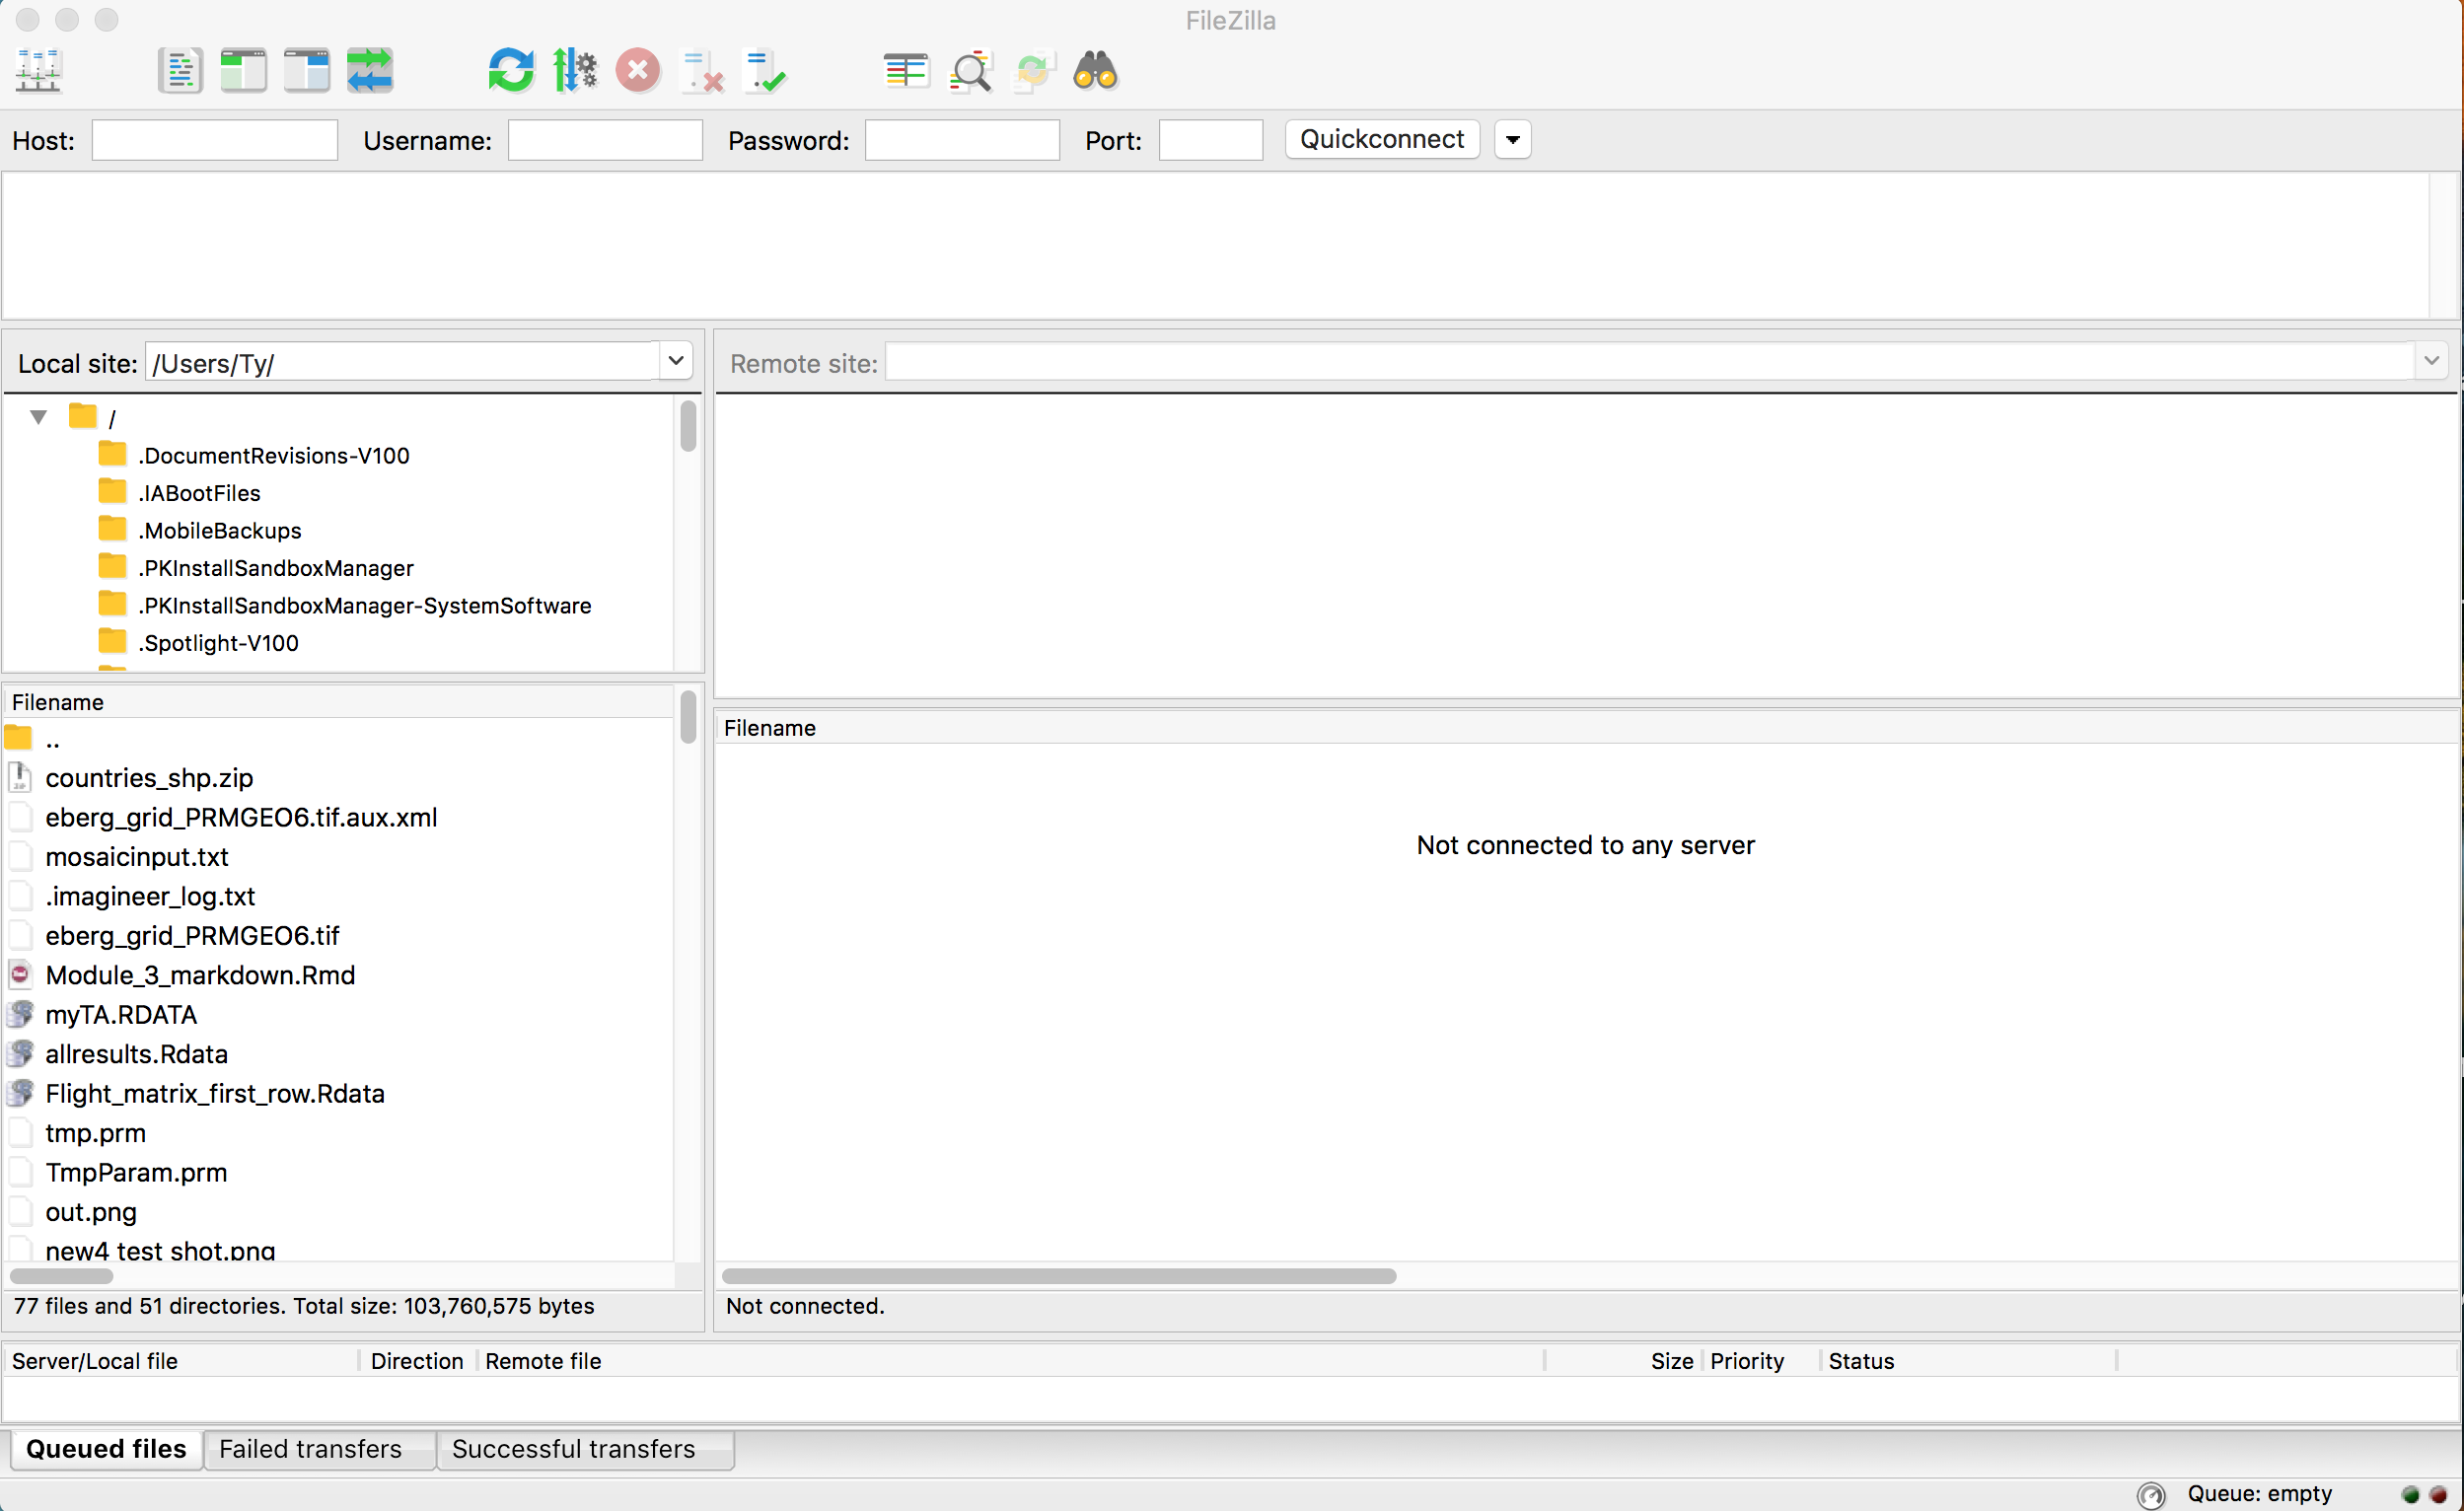
\includegraphics{Filezilla.png}
\caption{A fresh Filezilla window}
\end{figure}

\begin{figure}
\centering
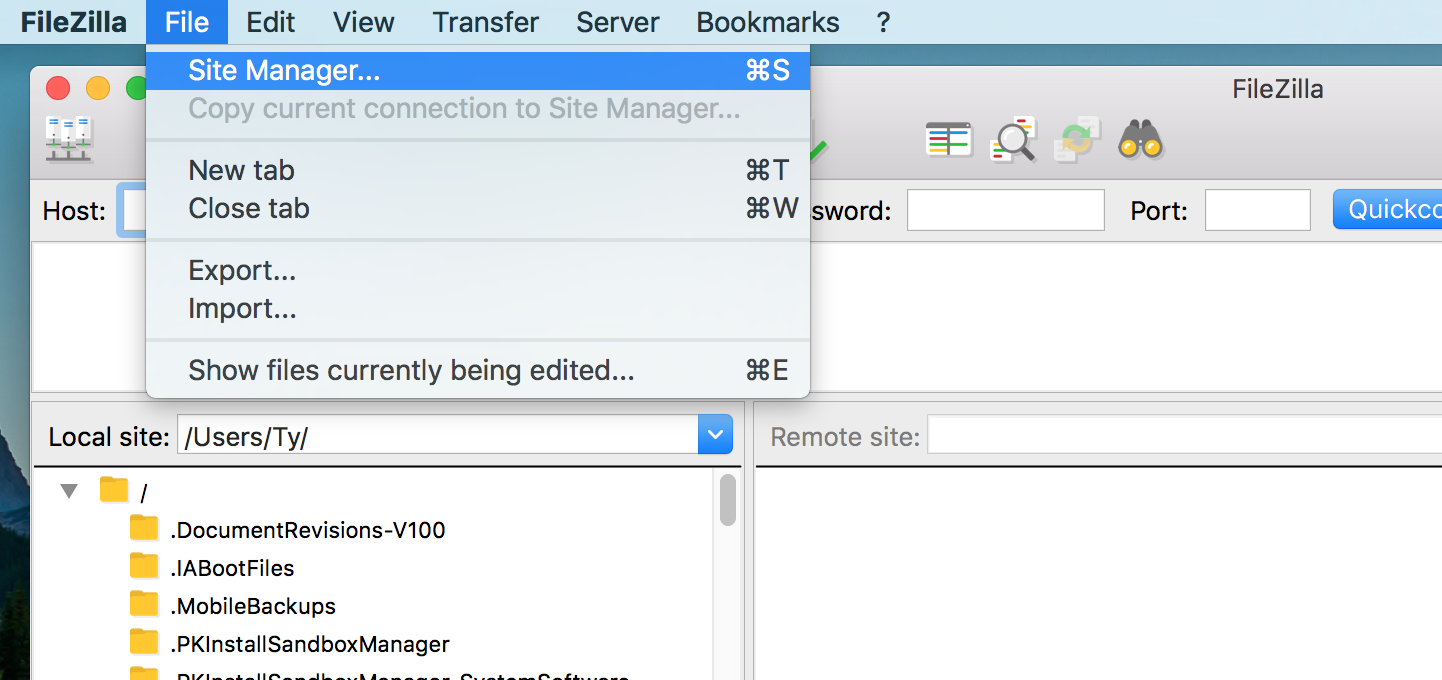
\includegraphics{site manager.png}
\caption{Start a new server link}
\end{figure}

\begin{figure}
\centering
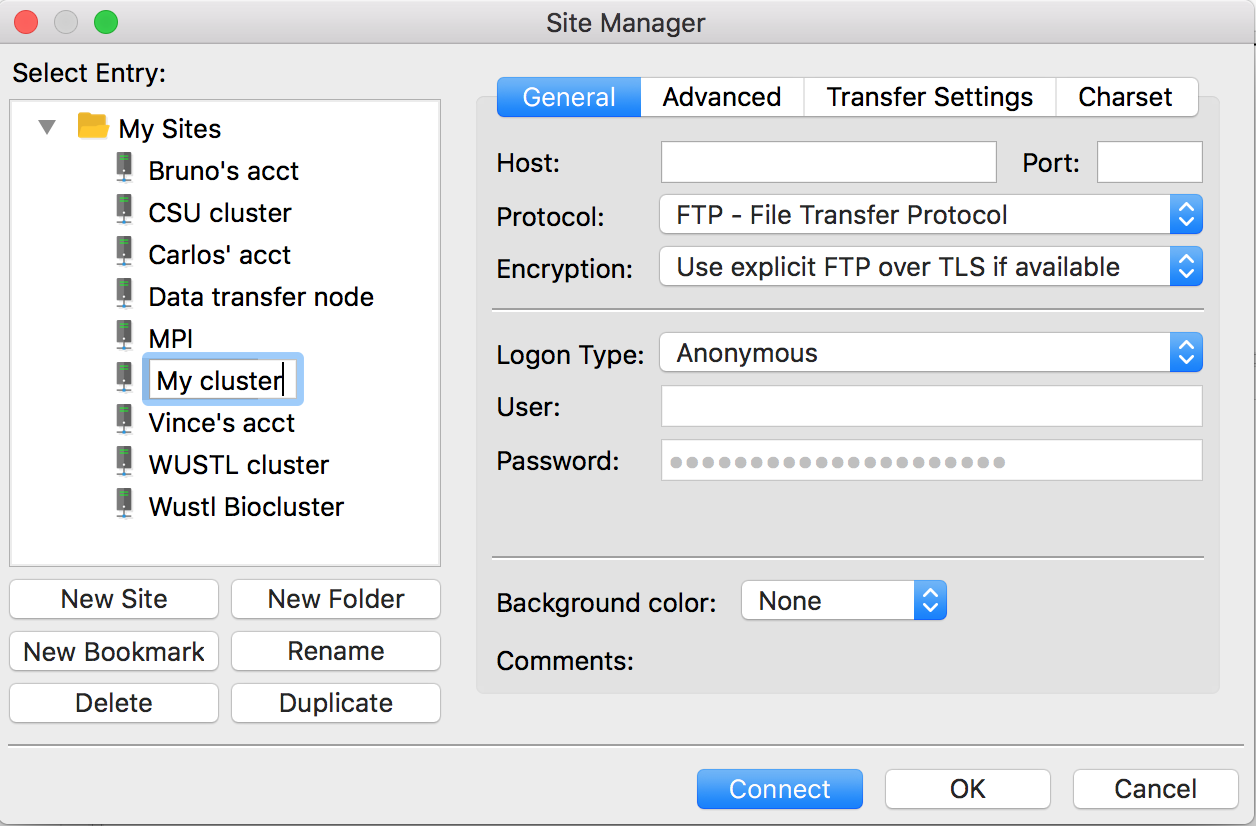
\includegraphics{New site name.png}
\caption{Start a new site and name that new site}
\end{figure}

\begin{figure}
\centering
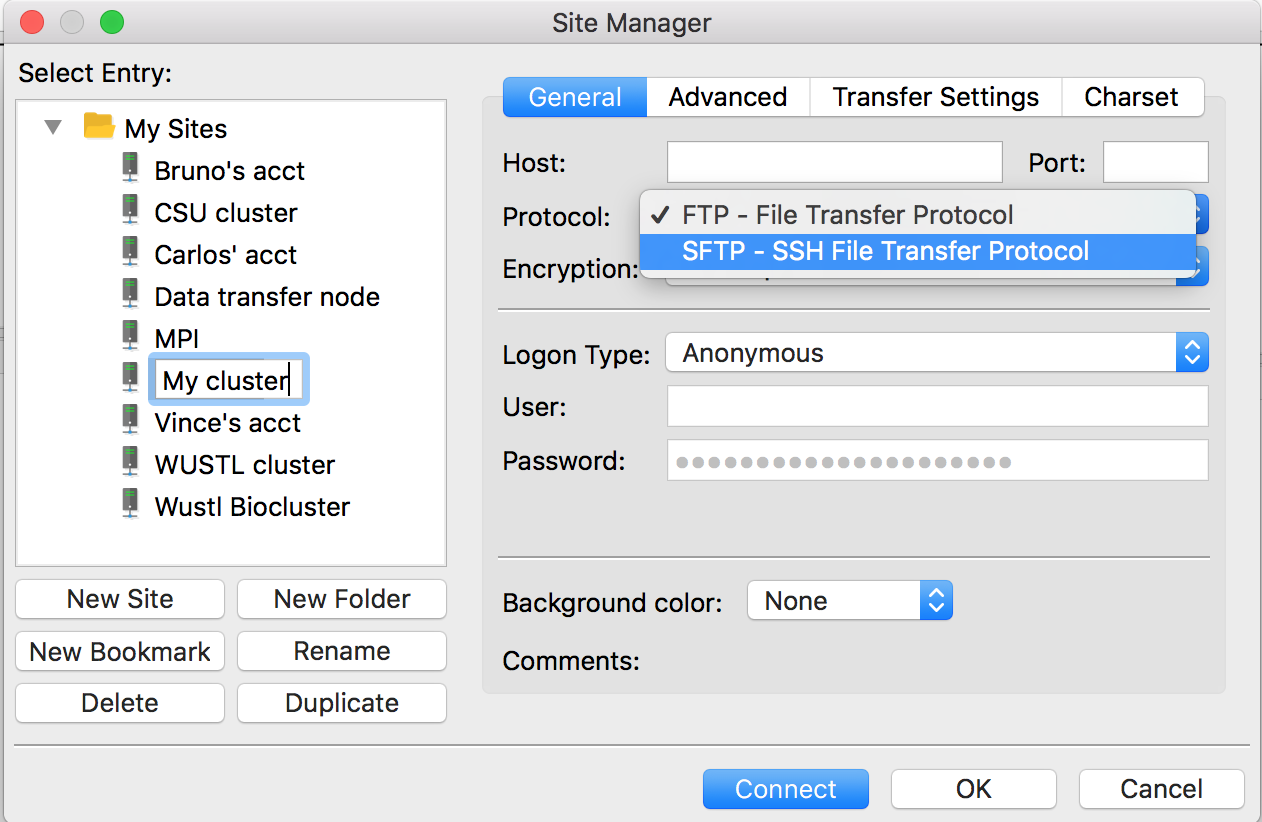
\includegraphics{SFTP.png}
\caption{Select a secure ssh file transfer protocol}
\end{figure}

\begin{figure}
\centering
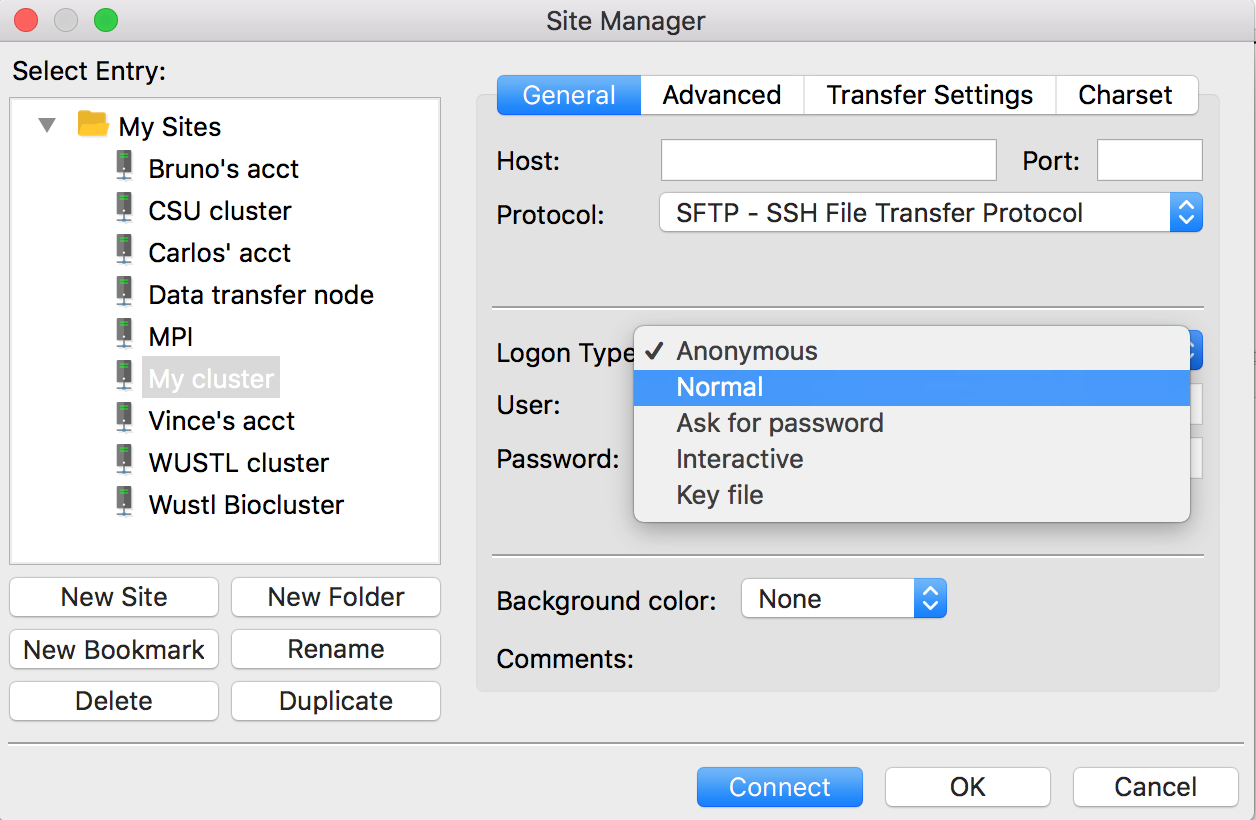
\includegraphics{Choose normal.png}
\caption{Login as normal}
\end{figure}

\begin{figure}
\centering
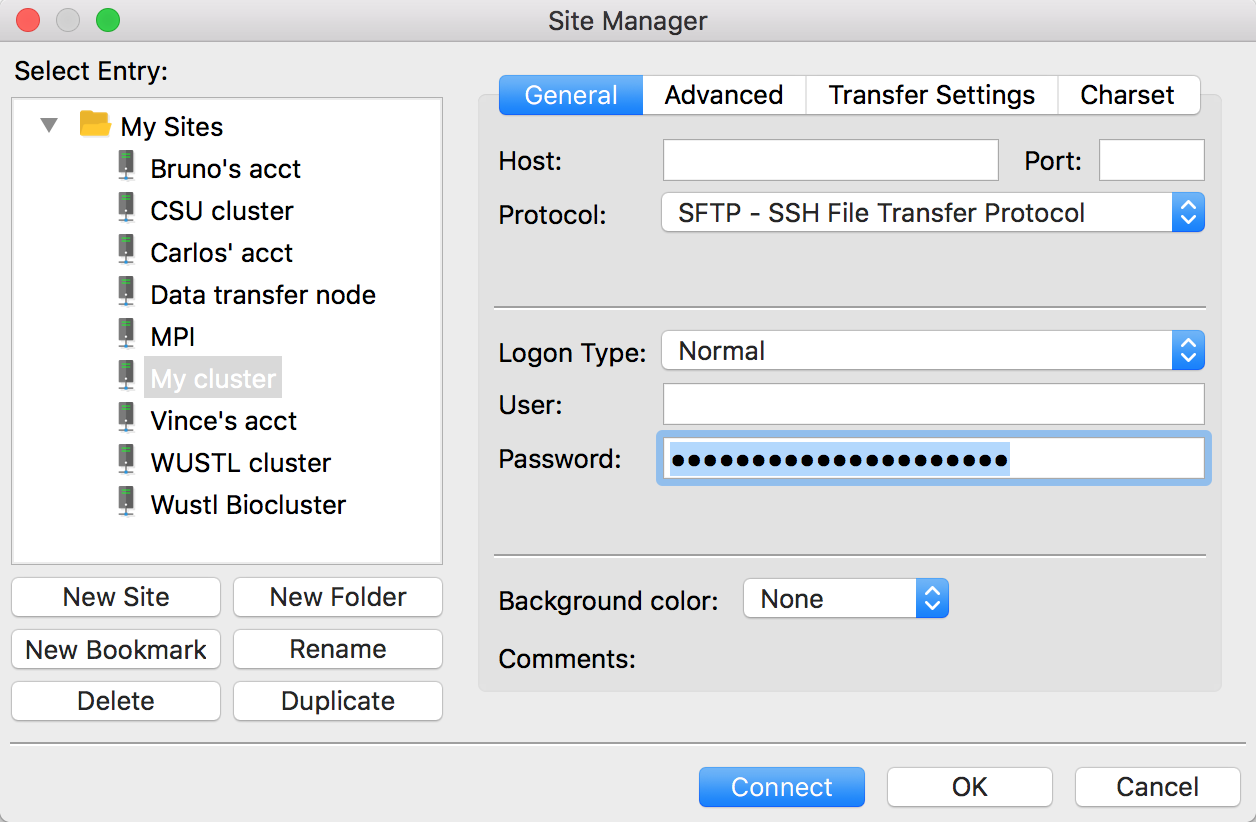
\includegraphics{Enter password.png}
\caption{Enter password}
\end{figure}

\begin{figure}
\centering
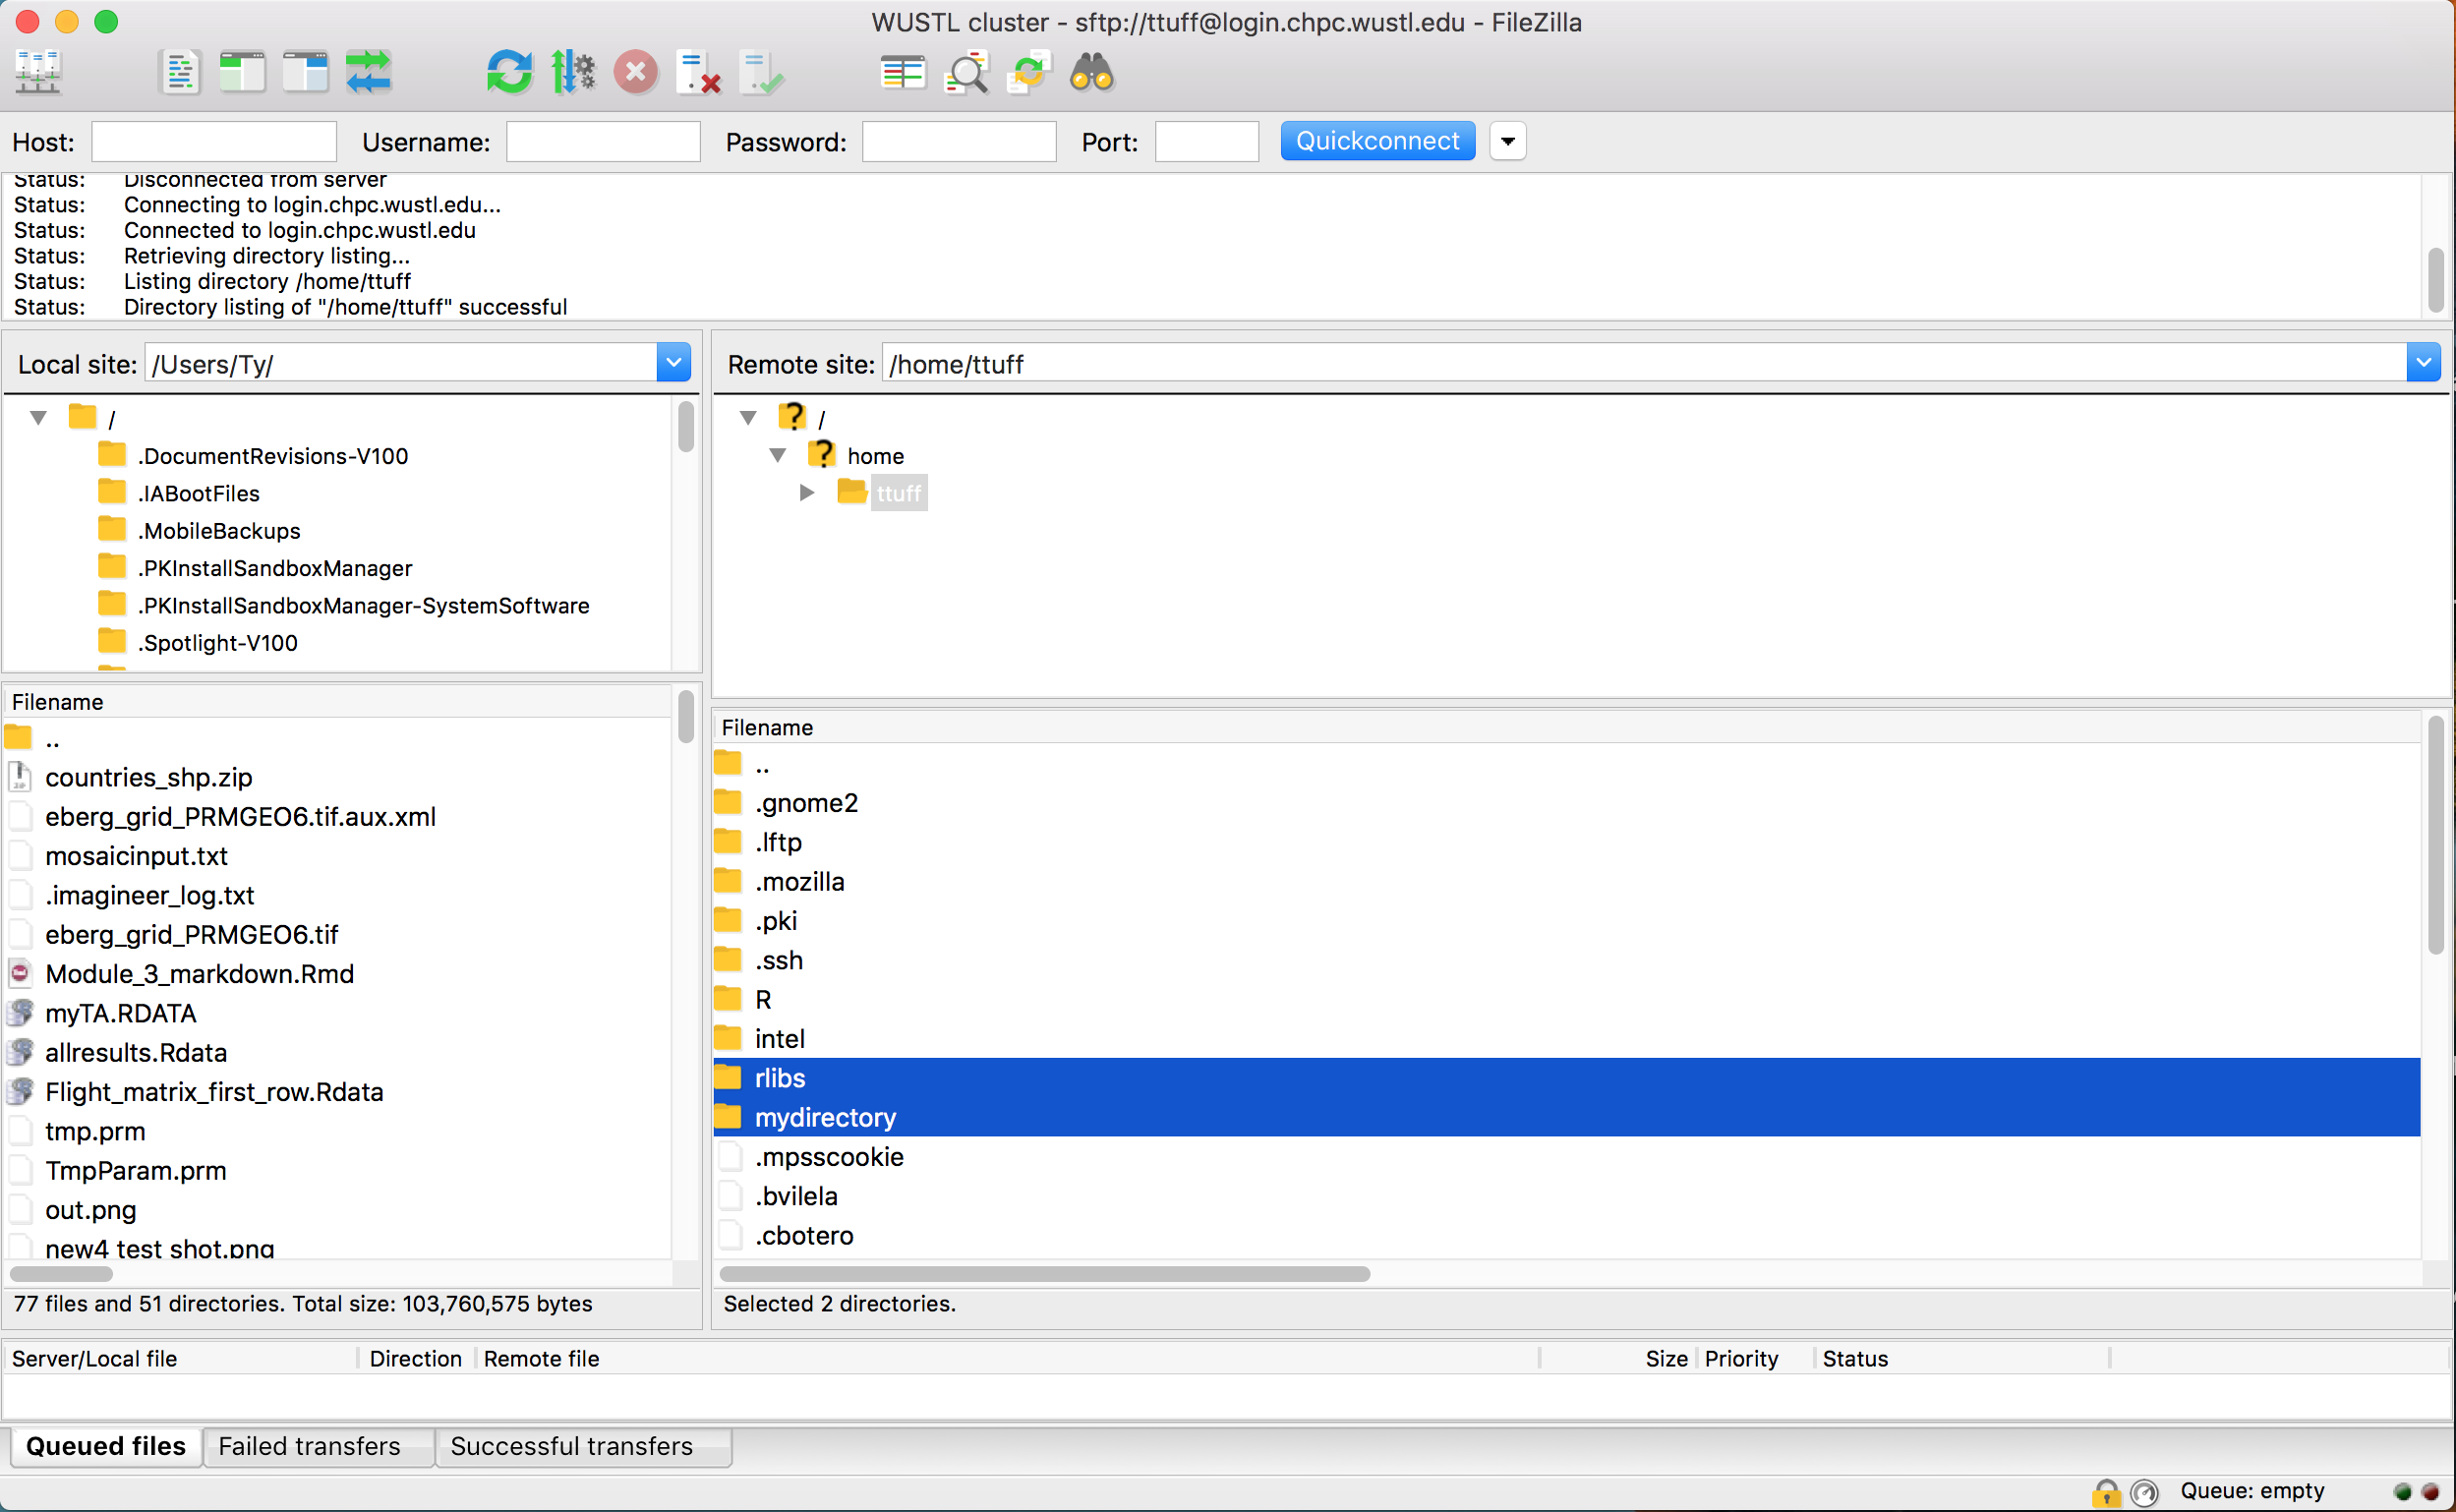
\includegraphics{Create two files within your home file.png}
\caption{You need to create two new directories (folders) for us to work
out of. Call one `rlibs' and the other `mydirectory'}
\end{figure}

\begin{figure}
\centering
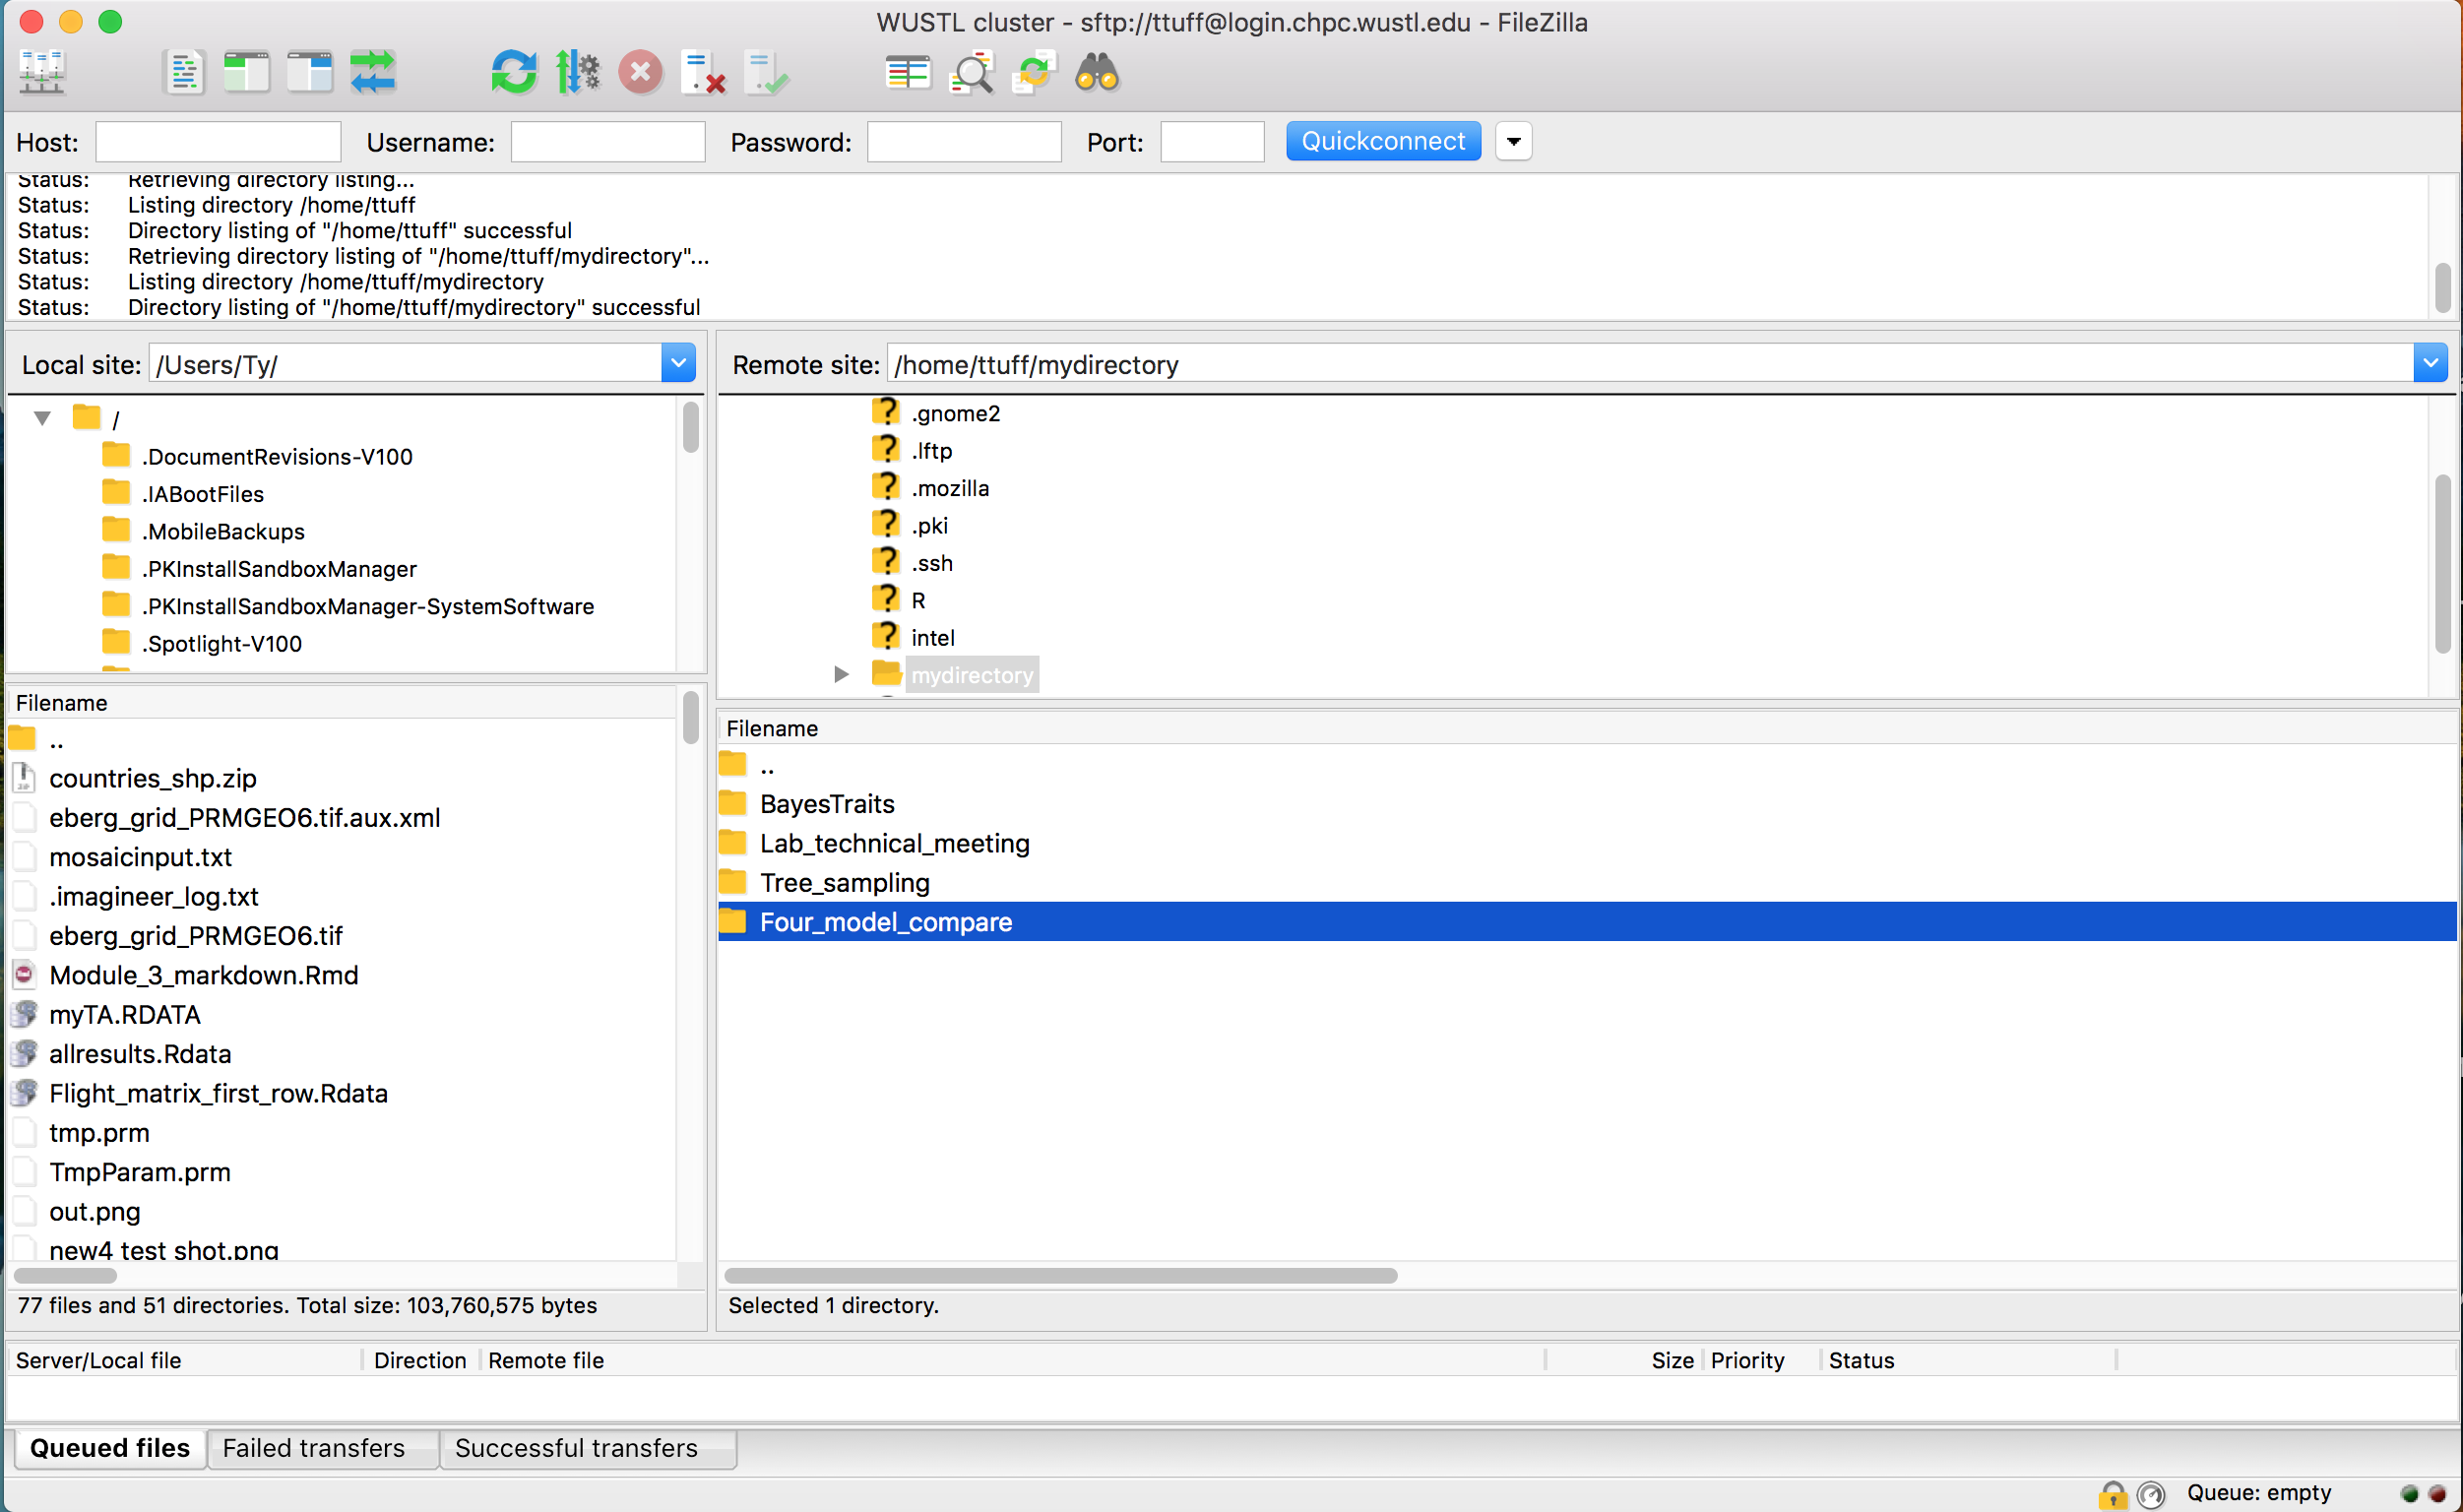
\includegraphics{Create Four_models_compare folder.png}
\caption{Within mydirectory, create another folder called
`Four\_model\_compare'}
\end{figure}

\begin{figure}
\centering
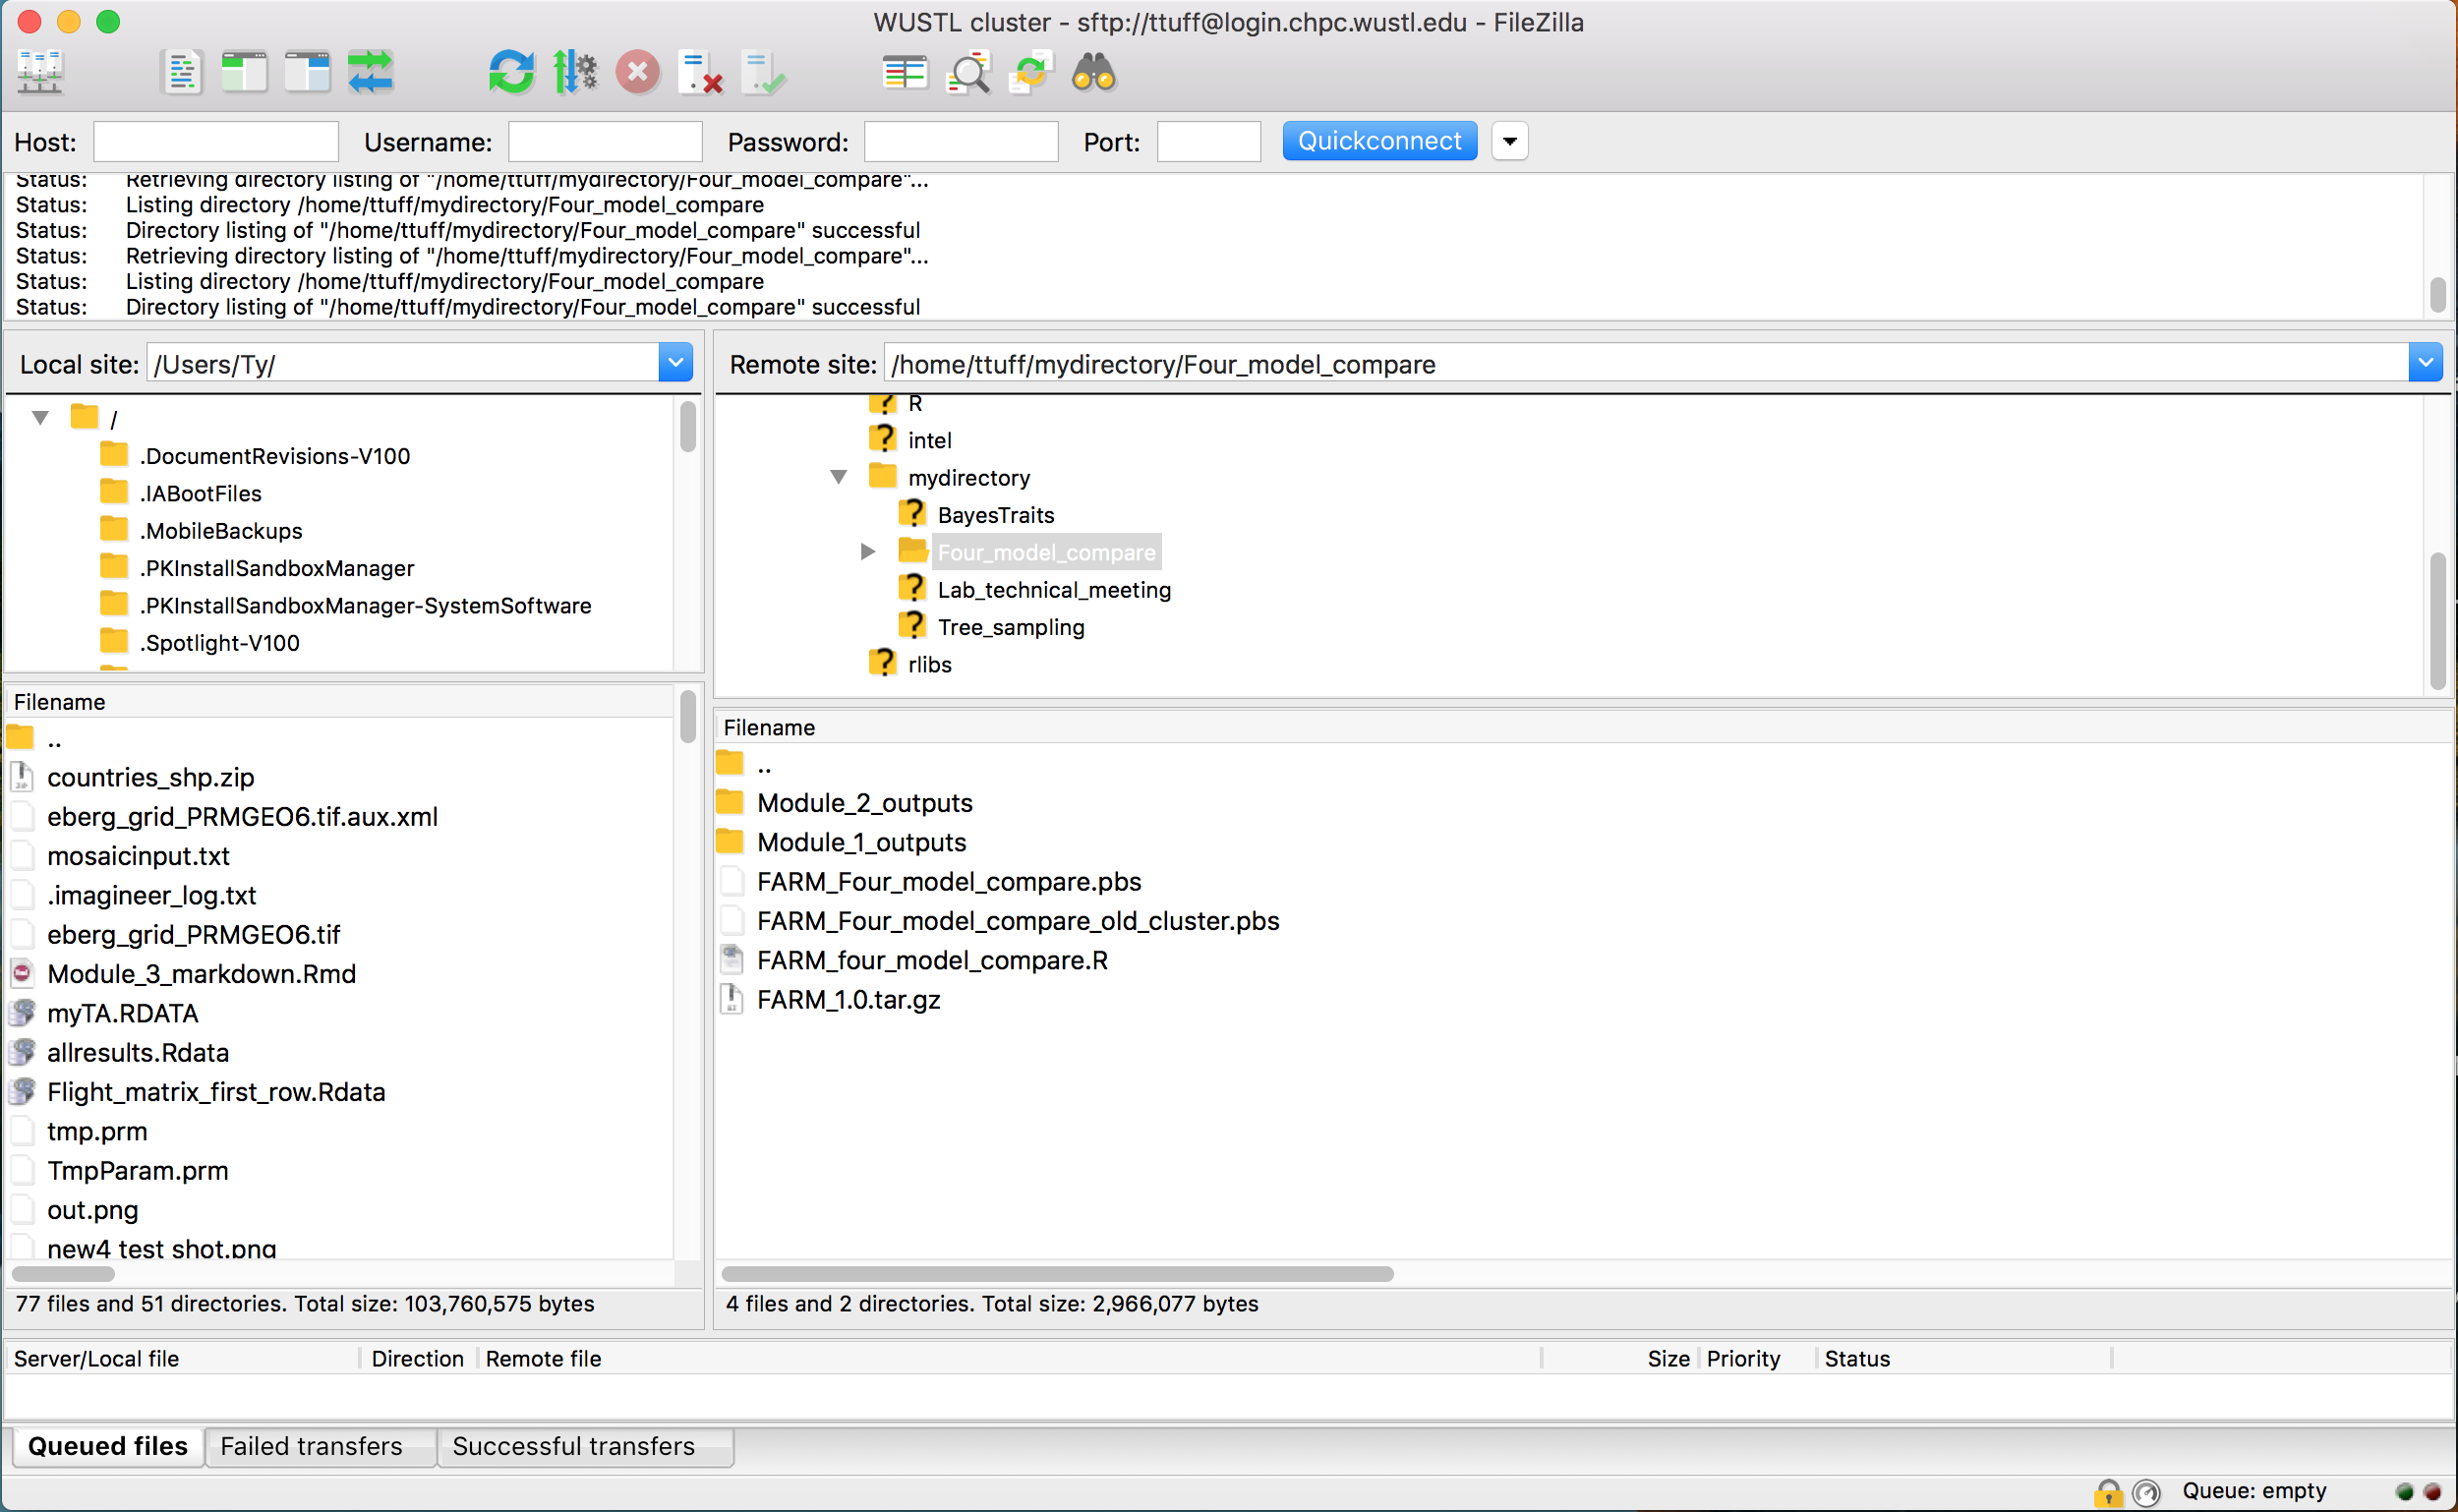
\includegraphics{Create module folders.png}
\caption{Within `Four\_model\_compare', create two folders called
`Module\_1\_outputs' and `Module\_2\_outputs'. Then drag three files
from your computer files on the left to the server folders on the right:
one .R file, one .pbs file, and a zip file with the package FARM in it.
These should be named FARM\_four\_model\_compare.R,
FARM\_four\_model\_compare\_old\_cluster.pbs, and FARM\_1.0.tar.gz .}
\end{figure}

Once logged in, you need to change the directory

\begin{Shaded}
\begin{Highlighting}[]
\BuiltInTok{cd}\NormalTok{ /home/ttuff/mydirectory/Four_model_compare}
\end{Highlighting}
\end{Shaded}

\begin{figure}
\centering
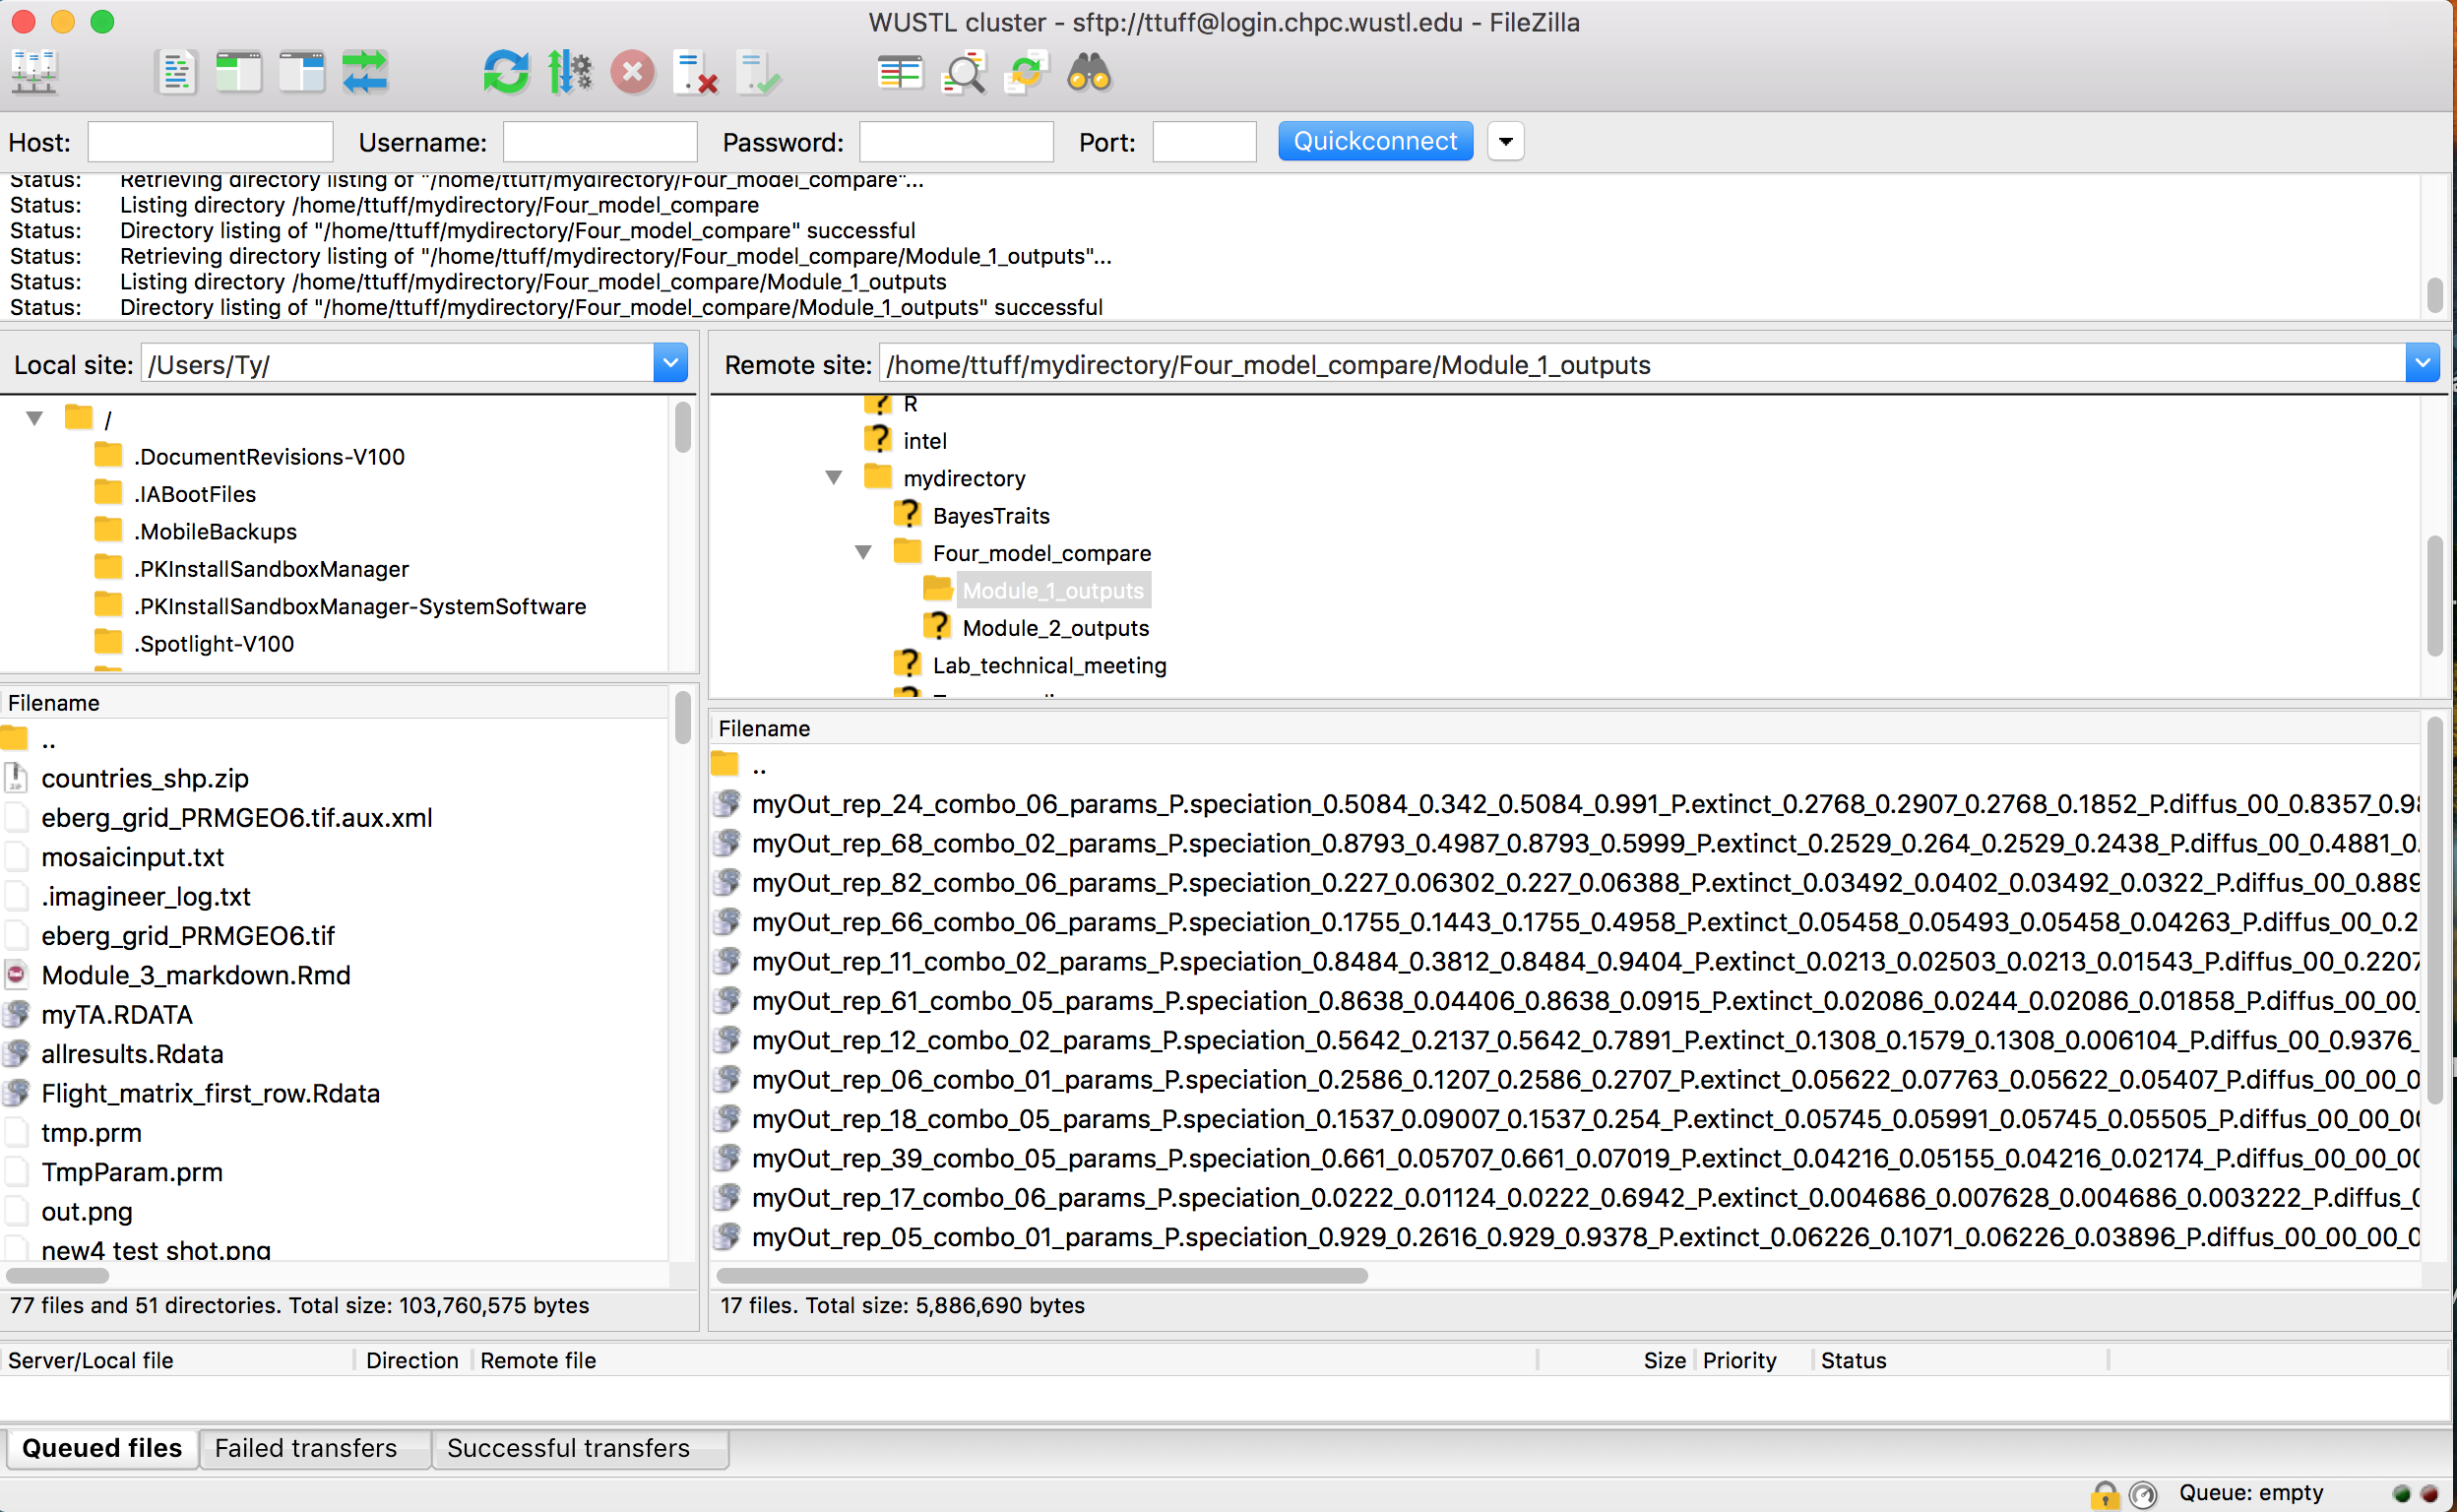
\includegraphics{Files from module 1.png}
\caption{}
\end{figure}

\begin{figure}
\centering
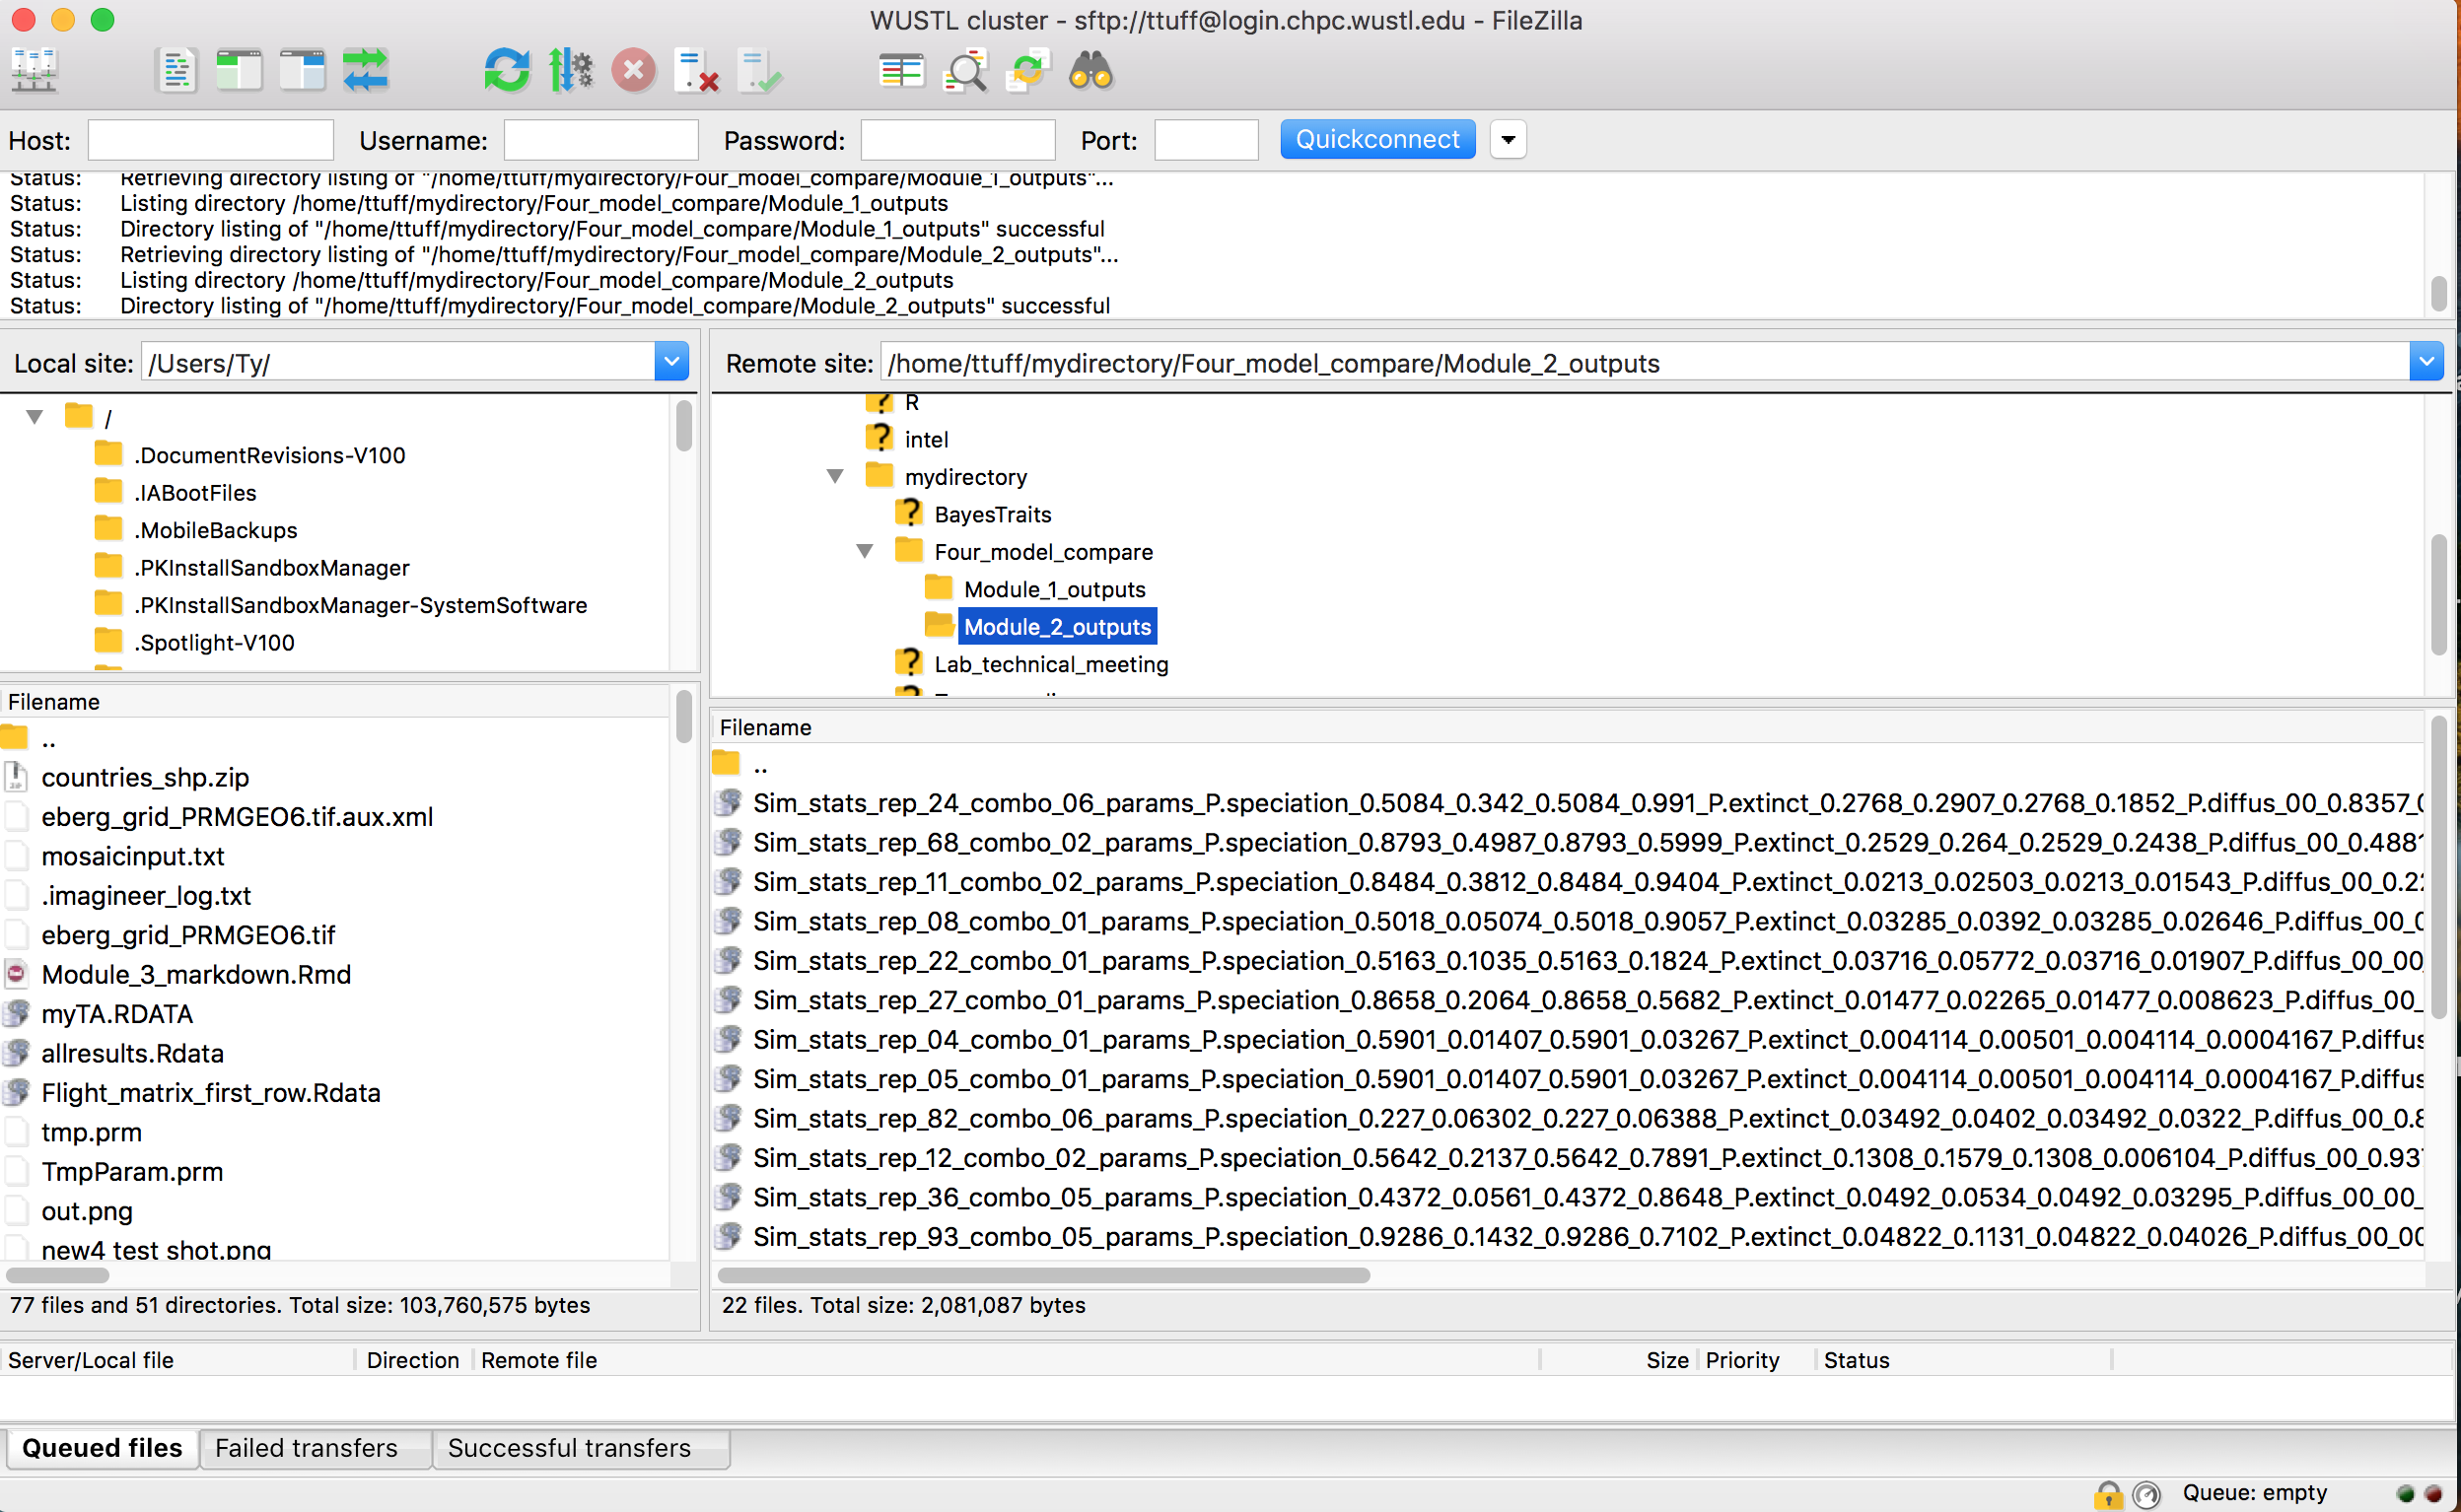
\includegraphics{Files from module 2.png}
\caption{}
\end{figure}

\chapter{Module 3: Analysing results produce from Modules 1 and
2}\label{module-3-analysing-results-produce-from-modules-1-and-2}

\begin{Shaded}
\begin{Highlighting}[]
\KeywordTok{library}\NormalTok{(png)}
\end{Highlighting}
\end{Shaded}

\section{Organize data}\label{organize-data}

\begin{Shaded}
\begin{Highlighting}[]
\CommentTok{# A frequent scenario in our analysis code is that we need to read thousands of }
\CommentTok{# output files into a single table. }
\CommentTok{# There are a couple flavors of file name that need to be dealt with and the }
\CommentTok{# output file needs to include a column with the full file name for reference }
\CommentTok{# later. We want to save the final table as it's own file to a folder outside of }
\CommentTok{# the one we just read. }

\NormalTok{## Here is one flaver where the input is two folders, one with extant }
\CommentTok{# simulations and one with extinct simulations. Need to read the files and }
\CommentTok{# produce two tables, one for extinct and one for extant. }

\NormalTok{## First consolidate the available files into a single table}
\NormalTok{concatenate <-}\StringTok{ }\ControlFlowTok{function}\NormalTok{(path) \{}
\NormalTok{ available <-}\StringTok{ }\KeywordTok{list.files}\NormalTok{(path, }\DataTypeTok{full.names =} \OtherTok{TRUE}\NormalTok{)}
\NormalTok{ name <-}\StringTok{ }\KeywordTok{unlist}\NormalTok{(}\KeywordTok{strsplit}\NormalTok{(available[}\DecValTok{1}\NormalTok{], }\DataTypeTok{split=}\StringTok{"_"}\NormalTok{))}
\NormalTok{ n <-}\StringTok{ }\KeywordTok{length}\NormalTok{(available)}
\NormalTok{ n_name <-}\StringTok{ }\KeywordTok{length}\NormalTok{(name) }\OperatorTok{-}\StringTok{ }\DecValTok{1}
 \KeywordTok{load}\NormalTok{(available[}\DecValTok{1}\NormalTok{])}
\NormalTok{ ncol_files <-}\StringTok{ }\KeywordTok{length}\NormalTok{(Sim_statistics[[}\DecValTok{1}\NormalTok{]]) }\OperatorTok{+}\StringTok{ }\NormalTok{n_name}
\NormalTok{ files <-}\StringTok{ }\KeywordTok{matrix}\NormalTok{(}\DataTypeTok{nrow =}\NormalTok{ n,}
                 \DataTypeTok{ncol =}\NormalTok{ ncol_files)}
\NormalTok{ split_names <-}\StringTok{ }\ControlFlowTok{function}\NormalTok{(x)\{}\KeywordTok{unlist}\NormalTok{(}\KeywordTok{strsplit}\NormalTok{(x, }\DataTypeTok{split =} \StringTok{"_"}\NormalTok{))\}}
\NormalTok{ name_available <-}\StringTok{ }\KeywordTok{do.call}\NormalTok{(rbind, }\KeywordTok{lapply}\NormalTok{(}\KeywordTok{as.list}\NormalTok{(available), split_names))}
\NormalTok{ files[, }\DecValTok{1}\OperatorTok{:}\NormalTok{n_name] <-}\StringTok{ }\NormalTok{name_available[, }\OperatorTok{-}\KeywordTok{ncol}\NormalTok{(name_available)]}

 \ControlFlowTok{for}\NormalTok{ (i }\ControlFlowTok{in} \DecValTok{1}\OperatorTok{:}\NormalTok{n) \{}
\NormalTok{   error <-}\StringTok{ }\KeywordTok{try}\NormalTok{(}\KeywordTok{load}\NormalTok{(available[i]), }\DataTypeTok{silent =} \OtherTok{TRUE}\NormalTok{)}
   \ControlFlowTok{if}\NormalTok{ (}\KeywordTok{class}\NormalTok{(error) }\OperatorTok{!=}\StringTok{ "try-error"}\NormalTok{) \{}
\NormalTok{     files[i, (n_name }\OperatorTok{+}\StringTok{ }\DecValTok{1}\NormalTok{)}\OperatorTok{:}\NormalTok{ncol_files] <-}\StringTok{ }\NormalTok{Sim_statistics[[}\DecValTok{1}\NormalTok{]]}
\NormalTok{   \}}
\NormalTok{ \}}


\NormalTok{ files <-}\StringTok{ }\NormalTok{files[, }\OperatorTok{-}\KeywordTok{c}\NormalTok{(}\DecValTok{1}\NormalTok{, }\DecValTok{2}\NormalTok{, }\DecValTok{3}\NormalTok{, }\DecValTok{5}\NormalTok{, }\DecValTok{7}\NormalTok{, }\DecValTok{8}\NormalTok{, }\DecValTok{13}\NormalTok{, }\DecValTok{18}\NormalTok{, }\DecValTok{23}\NormalTok{, }\DecValTok{28}\NormalTok{, }\DecValTok{33}\NormalTok{, }\DecValTok{35}\NormalTok{)]}
\NormalTok{ last_name <-}\StringTok{ }\KeywordTok{colnames}\NormalTok{(Sim_statistics[[}\DecValTok{1}\NormalTok{]])}
 \ControlFlowTok{if}\NormalTok{ (}\KeywordTok{is.null}\NormalTok{(last_name)) \{}

\NormalTok{   files <-}\StringTok{ }\NormalTok{files[, }\OperatorTok{-}\KeywordTok{ncol}\NormalTok{(files)]}
\NormalTok{ \}}
 \KeywordTok{colnames}\NormalTok{(files) <-}\StringTok{  }\KeywordTok{c}\NormalTok{(}\StringTok{"Sim_stats_rep"}\NormalTok{, }\StringTok{"combo"}\NormalTok{, }\KeywordTok{paste0}\NormalTok{(}\StringTok{"P.speciation"}\NormalTok{, }\DecValTok{1}\OperatorTok{:}\DecValTok{4}\NormalTok{),}
                       \KeywordTok{paste0}\NormalTok{(}\StringTok{"P.extinct"}\NormalTok{, }\DecValTok{1}\OperatorTok{:}\DecValTok{4}\NormalTok{),  }\KeywordTok{paste0}\NormalTok{(}\StringTok{"P.diffus"}\NormalTok{, }\DecValTok{1}\OperatorTok{:}\DecValTok{4}\NormalTok{),}
                       \KeywordTok{paste0}\NormalTok{(}\StringTok{"P.TO"}\NormalTok{, }\DecValTok{1}\OperatorTok{:}\DecValTok{4}\NormalTok{),  }\KeywordTok{paste0}\NormalTok{(}\StringTok{"P.Arisal"}\NormalTok{, }\DecValTok{1}\OperatorTok{:}\DecValTok{4}\NormalTok{), }
                       \StringTok{"timesteps"}\NormalTok{, }\StringTok{"NBS"}\NormalTok{, last_name)}

\NormalTok{ Concatenated_data <-}\StringTok{ }\KeywordTok{as.data.frame}\NormalTok{(files)}

\NormalTok{ begin <-}\StringTok{ }\KeywordTok{which}\NormalTok{(}\KeywordTok{colnames}\NormalTok{(Concatenated_data) }\OperatorTok{==}\StringTok{  "number_of_branches"}\NormalTok{)}
\NormalTok{ Concatenated_data_stat <-}\StringTok{ }\NormalTok{Concatenated_data[, begin}\OperatorTok{:}\KeywordTok{ncol}\NormalTok{(Concatenated_data)]}
\NormalTok{ Concatenated_data_stat <-}\StringTok{ }\KeywordTok{apply}\NormalTok{(Concatenated_data_stat, }\DecValTok{2}\NormalTok{, as.numeric)}
\NormalTok{ remove <-}\StringTok{ }\KeywordTok{which}\NormalTok{(}\KeywordTok{is.na}\NormalTok{(}\KeywordTok{rowSums}\NormalTok{(Concatenated_data_stat)))}
\NormalTok{ Concatenated_data <-}\StringTok{ }\NormalTok{Concatenated_data[}\OperatorTok{-}\NormalTok{remove, ]}

\NormalTok{ one <-}\StringTok{ }\KeywordTok{subset}\NormalTok{(Concatenated_data, combo }\OperatorTok{==}\StringTok{"01"}\NormalTok{)}
\NormalTok{ two <-}\StringTok{ }\KeywordTok{subset}\NormalTok{(Concatenated_data, combo }\OperatorTok{==}\StringTok{"02"}\NormalTok{)}
\NormalTok{ five <-}\StringTok{ }\KeywordTok{subset}\NormalTok{(Concatenated_data, combo }\OperatorTok{==}\StringTok{"05"}\NormalTok{)}
\NormalTok{ six <-}\StringTok{ }\KeywordTok{subset}\NormalTok{(Concatenated_data, combo }\OperatorTok{==}\StringTok{"06"}\NormalTok{)}

\NormalTok{ crop <-}\StringTok{ }\KeywordTok{min}\NormalTok{(}\KeywordTok{sapply}\NormalTok{(}\KeywordTok{list}\NormalTok{(one, two, five, six), nrow))}

\NormalTok{ one <-}\StringTok{ }\NormalTok{one[}\DecValTok{1}\OperatorTok{:}\NormalTok{crop, ]}
\NormalTok{ two <-}\StringTok{ }\NormalTok{two[}\DecValTok{1}\OperatorTok{:}\NormalTok{crop, ]}
\NormalTok{ five <-}\StringTok{ }\NormalTok{five[}\DecValTok{1}\OperatorTok{:}\NormalTok{crop, ]}
\NormalTok{ six <-}\StringTok{ }\NormalTok{six[}\DecValTok{1}\OperatorTok{:}\NormalTok{crop, ]}

\NormalTok{ Concatenated_data2 <-}\StringTok{ }\KeywordTok{rbind}\NormalTok{(one, two, five, six)}
\NormalTok{ res <-}\StringTok{ }\KeywordTok{list}\NormalTok{(Concatenated_data, Concatenated_data2, crop)}
 \KeywordTok{names}\NormalTok{(res) <-}\StringTok{ }\KeywordTok{c}\NormalTok{(}\StringTok{"Concatenated_data"}\NormalTok{, }\StringTok{"Concatenated_data_crop"}\NormalTok{, }\StringTok{"crop"}\NormalTok{)}
 \KeywordTok{return}\NormalTok{(res)}
 
\NormalTok{\}}

\NormalTok{path <-}\StringTok{ "~/Box Sync/Four model compare third run/Module 2"}
\NormalTok{Concatenated_data0 <-}\StringTok{ }\KeywordTok{concatenate}\NormalTok{(path)}
\KeywordTok{print}\NormalTok{(Concatenated_data0[[}\DecValTok{3}\NormalTok{]])}
\NormalTok{path_save <-}\StringTok{ "~/Box Sync/Four model compare third run"}
\NormalTok{Concatenated_data <-}\StringTok{ }\NormalTok{Concatenated_data0[[}\DecValTok{1}\NormalTok{]]}
\KeywordTok{save}\NormalTok{(Concatenated_data, }\DataTypeTok{file =} \KeywordTok{paste0}\NormalTok{(path_save,}
                                     \StringTok{"/Four_model_compare_results_not_cropped.Rdata"}\NormalTok{))}
\NormalTok{Concatenated_data <-}\StringTok{ }\NormalTok{Concatenated_data0[[}\DecValTok{2}\NormalTok{]]}
\KeywordTok{save}\NormalTok{(Concatenated_data, }\DataTypeTok{file=}\KeywordTok{paste0}\NormalTok{(path_save,}
                                   \StringTok{"/Four_model_compare_results_"}\NormalTok{, }
                                   \KeywordTok{format}\NormalTok{(}\KeywordTok{Sys.time}\NormalTok{(), }\DataTypeTok{format=}\StringTok{"%d_%b_%Y"}\NormalTok{),}
                                   \StringTok{"_crop_to_"}\NormalTok{, Concatenated_data0[[}\DecValTok{3}\NormalTok{]],}\StringTok{".Rdata"}\NormalTok{))}

\NormalTok{### Repeated for extinct}
\NormalTok{path <-}\StringTok{ "~/Box Sync/Four model compare third run/Module 2 extinct"}
\NormalTok{Concatenated_data <-}\StringTok{ }\KeywordTok{concatenate}\NormalTok{(path)[[}\DecValTok{1}\NormalTok{]]}
\NormalTok{path_save <-}\StringTok{ "~/Box Sync/Four model compare third run"}

\KeywordTok{save}\NormalTok{(Concatenated_data, }\DataTypeTok{file=}\KeywordTok{paste0}\NormalTok{(path_save,}
                                   \StringTok{"/Four_model_compare_results_extinct_"}\NormalTok{, }
                                   \KeywordTok{format}\NormalTok{(}\KeywordTok{Sys.time}\NormalTok{(), }\DataTypeTok{format=}\StringTok{"%d_%b_%Y"}\NormalTok{),}\StringTok{".Rdata"}\NormalTok{))}
\end{Highlighting}
\end{Shaded}

\section{Diagnostics}\label{diagnostics}

\begin{Shaded}
\begin{Highlighting}[]
\KeywordTok{load}\NormalTok{(}\StringTok{"Four_model_compare_results_02_Aug_2017_crop_to_6128.Rdata"}\NormalTok{)}
\NormalTok{extant <-}\StringTok{ }\NormalTok{Concatenated_data}
\NormalTok{extant}

 \KeywordTok{load}\NormalTok{(}\StringTok{"Four_model_compare_results_extinct_02_Aug_2017.Rdata"}\NormalTok{)}
\NormalTok{extinct <-}\StringTok{ }\NormalTok{Concatenated_data}
\NormalTok{extinct}

\KeywordTok{head}\NormalTok{(extant)}
\KeywordTok{head}\NormalTok{(extinct)}
\end{Highlighting}
\end{Shaded}

\begin{Shaded}
\begin{Highlighting}[]
\ControlFlowTok{for}\NormalTok{(i }\ControlFlowTok{in} \KeywordTok{c}\NormalTok{(}\DecValTok{3}\OperatorTok{:}\DecValTok{22}\NormalTok{))\{}
\NormalTok{    extinct[}\KeywordTok{which}\NormalTok{(}\KeywordTok{is.nan}\NormalTok{(}\KeywordTok{as.numeric}\NormalTok{(}\KeywordTok{as.character}\NormalTok{(extinct[, i]))) }\OperatorTok{==}\StringTok{ }\OtherTok{TRUE}\NormalTok{), i] <-}\StringTok{ }\OtherTok{NA}
\NormalTok{\}}

\ControlFlowTok{for}\NormalTok{(i }\ControlFlowTok{in} \KeywordTok{c}\NormalTok{(}\DecValTok{3}\OperatorTok{:}\DecValTok{22}\NormalTok{))\{}
\NormalTok{    extant[}\KeywordTok{which}\NormalTok{(}\KeywordTok{is.nan}\NormalTok{(}\KeywordTok{as.numeric}\NormalTok{(}\KeywordTok{as.character}\NormalTok{(extant[, i]))) }\OperatorTok{==}\StringTok{ }\OtherTok{TRUE}\NormalTok{), i] <-}\StringTok{ }\OtherTok{NA}
\NormalTok{\}}




\NormalTok{xlimit <-}\StringTok{ }\KeywordTok{c}\NormalTok{(}\DecValTok{0}\NormalTok{,}\DecValTok{1}\NormalTok{)}
\NormalTok{ylimit <-}\StringTok{ }\KeywordTok{c}\NormalTok{(}\DecValTok{0}\NormalTok{,}\DecValTok{3000}\NormalTok{)}
\NormalTok{maincex <-}\StringTok{ }\FloatTok{0.9}

\KeywordTok{png}\NormalTok{(}\DataTypeTok{file=}\StringTok{"Global_success_rate_per_parameter.png"}\NormalTok{, }\DataTypeTok{width=}\FloatTok{8.5}\NormalTok{, }\DataTypeTok{height=}\DecValTok{11}\NormalTok{, }\DataTypeTok{units=}\StringTok{"in"}\NormalTok{, }\DataTypeTok{res=}\DecValTok{300}\NormalTok{)}

\KeywordTok{par}\NormalTok{(}\DataTypeTok{mfrow=}\KeywordTok{c}\NormalTok{(}\DecValTok{5}\NormalTok{,}\DecValTok{4}\NormalTok{), }\DataTypeTok{mar=}\KeywordTok{c}\NormalTok{(}\DecValTok{3}\NormalTok{,}\DecValTok{3}\NormalTok{,}\DecValTok{3}\NormalTok{,}\DecValTok{0}\NormalTok{))}


\KeywordTok{hist}\NormalTok{(}\KeywordTok{as.numeric}\NormalTok{(}\KeywordTok{as.character}\NormalTok{(extinct[,}\DecValTok{3}\NormalTok{])), }\DataTypeTok{main=}\StringTok{"speciation of F in F env"}\NormalTok{, }\DataTypeTok{col=}\KeywordTok{adjustcolor}\NormalTok{(}\StringTok{"firebrick"}\NormalTok{, }\DataTypeTok{alpha=}\FloatTok{0.7}\NormalTok{), }\DataTypeTok{breaks=}\DecValTok{100}\NormalTok{, }\DataTypeTok{border=}\OtherTok{NA}\NormalTok{, }\DataTypeTok{xlim=}\NormalTok{ xlimit, }\DataTypeTok{ylim=}\NormalTok{ ylimit, }\DataTypeTok{cex.main=}\NormalTok{ maincex)}
\KeywordTok{hist}\NormalTok{(}\KeywordTok{as.numeric}\NormalTok{(}\KeywordTok{as.character}\NormalTok{(extant[,}\DecValTok{3}\NormalTok{])), }\DataTypeTok{main=}\StringTok{"speciation of F in F env"}\NormalTok{, }\DataTypeTok{col=}\KeywordTok{adjustcolor}\NormalTok{(}\StringTok{"cornflowerblue"}\NormalTok{, }\DataTypeTok{alpha=}\FloatTok{0.7}\NormalTok{), }\DataTypeTok{breaks=}\DecValTok{100}\NormalTok{, }\DataTypeTok{border=}\OtherTok{NA}\NormalTok{, }\DataTypeTok{xlim=}\NormalTok{ xlimit, }\DataTypeTok{ylim=}\NormalTok{ ylimit, }\DataTypeTok{cex.main=}\NormalTok{ maincex, }\DataTypeTok{add=}\OtherTok{TRUE}\NormalTok{)}


\KeywordTok{hist}\NormalTok{(}\KeywordTok{as.numeric}\NormalTok{(}\KeywordTok{as.character}\NormalTok{(extinct[,}\DecValTok{4}\NormalTok{])), }\DataTypeTok{main=}\StringTok{"speciation of D in F env"}\NormalTok{, }\DataTypeTok{col=}\KeywordTok{adjustcolor}\NormalTok{(}\StringTok{"firebrick"}\NormalTok{, }\DataTypeTok{alpha=} \FloatTok{0.7}\NormalTok{), }\DataTypeTok{breaks=}\DecValTok{100}\NormalTok{, }\DataTypeTok{border=}\OtherTok{NA}\NormalTok{, }\DataTypeTok{xlim=}\NormalTok{ xlimit, }\DataTypeTok{ylim=}\NormalTok{ ylimit, }\DataTypeTok{cex.main=}\NormalTok{ maincex)}
\KeywordTok{hist}\NormalTok{(}\KeywordTok{as.numeric}\NormalTok{(}\KeywordTok{as.character}\NormalTok{(extant[,}\DecValTok{4}\NormalTok{])), }\DataTypeTok{main=}\StringTok{"speciation of D in F env"}\NormalTok{, }\DataTypeTok{col=}\KeywordTok{adjustcolor}\NormalTok{(}\StringTok{"cornflowerblue"}\NormalTok{, }\DataTypeTok{alpha=} \FloatTok{0.7}\NormalTok{), }\DataTypeTok{breaks=}\DecValTok{100}\NormalTok{, }\DataTypeTok{border=}\OtherTok{NA}\NormalTok{, }\DataTypeTok{xlim=}\NormalTok{ xlimit, }\DataTypeTok{ylim=}\NormalTok{ ylimit, }\DataTypeTok{cex.main=}\NormalTok{ maincex, }\DataTypeTok{add=}\OtherTok{TRUE}\NormalTok{)}


\KeywordTok{hist}\NormalTok{(}\KeywordTok{as.numeric}\NormalTok{(}\KeywordTok{as.character}\NormalTok{(extinct[,}\DecValTok{5}\NormalTok{])), }\DataTypeTok{main=}\StringTok{"speciation of F in D env"}\NormalTok{, }\DataTypeTok{col=}\KeywordTok{adjustcolor}\NormalTok{(}\StringTok{"firebrick"}\NormalTok{, }\DataTypeTok{alpha=} \FloatTok{0.7}\NormalTok{), }\DataTypeTok{breaks=}\DecValTok{100}\NormalTok{, }\DataTypeTok{border=}\OtherTok{NA}\NormalTok{, }\DataTypeTok{xlim=}\NormalTok{ xlimit, }\DataTypeTok{ylim=}\NormalTok{ ylimit, }\DataTypeTok{cex.main=}\NormalTok{ maincex)}
\KeywordTok{hist}\NormalTok{(}\KeywordTok{as.numeric}\NormalTok{(}\KeywordTok{as.character}\NormalTok{(extant[,}\DecValTok{5}\NormalTok{])), }\DataTypeTok{main=}\StringTok{"speciation of F in D env"}\NormalTok{, }\DataTypeTok{col=}\KeywordTok{adjustcolor}\NormalTok{(}\StringTok{"cornflowerblue"}\NormalTok{, }\DataTypeTok{alpha=} \FloatTok{0.7}\NormalTok{), }\DataTypeTok{breaks=}\DecValTok{100}\NormalTok{, }\DataTypeTok{border=}\OtherTok{NA}\NormalTok{, }\DataTypeTok{xlim=}\NormalTok{ xlimit, }\DataTypeTok{ylim=}\NormalTok{ ylimit, }\DataTypeTok{cex.main=}\NormalTok{ maincex, }\DataTypeTok{add=}\OtherTok{TRUE}\NormalTok{)}

\KeywordTok{hist}\NormalTok{(}\KeywordTok{as.numeric}\NormalTok{(}\KeywordTok{as.character}\NormalTok{(extinct[,}\DecValTok{6}\NormalTok{])), }\DataTypeTok{main=}\StringTok{"speciation of D in D env"}\NormalTok{, }\DataTypeTok{col=}\KeywordTok{adjustcolor}\NormalTok{(}\StringTok{"firebrick"}\NormalTok{, }\DataTypeTok{alpha=} \FloatTok{0.7}\NormalTok{), }\DataTypeTok{breaks=}\DecValTok{100}\NormalTok{, }\DataTypeTok{border=}\OtherTok{NA}\NormalTok{, }\DataTypeTok{xlim=}\NormalTok{ xlimit, }\DataTypeTok{ylim=}\NormalTok{ ylimit, }\DataTypeTok{cex.main=}\NormalTok{ maincex)}
\KeywordTok{hist}\NormalTok{(}\KeywordTok{as.numeric}\NormalTok{(}\KeywordTok{as.character}\NormalTok{(extant[,}\DecValTok{6}\NormalTok{])), }\DataTypeTok{main=}\StringTok{"speciation of D in D env"}\NormalTok{, }\DataTypeTok{col=}\KeywordTok{adjustcolor}\NormalTok{(}\StringTok{"cornflowerblue"}\NormalTok{, }\DataTypeTok{alpha=} \FloatTok{0.7}\NormalTok{), }\DataTypeTok{breaks=}\DecValTok{100}\NormalTok{, }\DataTypeTok{border=}\OtherTok{NA}\NormalTok{, }\DataTypeTok{xlim=}\NormalTok{ xlimit, }\DataTypeTok{ylim=}\NormalTok{ ylimit, }\DataTypeTok{cex.main=}\NormalTok{ maincex, }\DataTypeTok{add=}\OtherTok{TRUE}\NormalTok{)}

\NormalTok{#######}

\KeywordTok{hist}\NormalTok{(}\KeywordTok{as.numeric}\NormalTok{(}\KeywordTok{as.character}\NormalTok{(extinct[, }\DecValTok{7}\NormalTok{])), }\DataTypeTok{main=}\StringTok{"extinction of F in F env"}\NormalTok{, }\DataTypeTok{col=}\KeywordTok{adjustcolor}\NormalTok{(}\StringTok{"firebrick"}\NormalTok{, }\DataTypeTok{alpha=} \FloatTok{0.7}\NormalTok{), }\DataTypeTok{breaks=}\DecValTok{100}\NormalTok{, }\DataTypeTok{border=}\OtherTok{NA}\NormalTok{, }\DataTypeTok{xlim=}\NormalTok{ xlimit, }\DataTypeTok{ylim=}\NormalTok{ ylimit, }\DataTypeTok{cex.main=}\NormalTok{ maincex)}
\KeywordTok{hist}\NormalTok{(}\KeywordTok{as.numeric}\NormalTok{(}\KeywordTok{as.character}\NormalTok{(extant[, }\DecValTok{7}\NormalTok{])), }\DataTypeTok{main=}\StringTok{"extinction of F in F env"}\NormalTok{, }\DataTypeTok{col=}\KeywordTok{adjustcolor}\NormalTok{(}\StringTok{"cornflowerblue"}\NormalTok{, }\DataTypeTok{alpha=} \FloatTok{0.7}\NormalTok{), }\DataTypeTok{breaks=}\DecValTok{100}\NormalTok{, }\DataTypeTok{border=}\OtherTok{NA}\NormalTok{, }\DataTypeTok{xlim=}\NormalTok{ xlimit, }\DataTypeTok{ylim=}\NormalTok{ ylimit, }\DataTypeTok{cex.main=}\NormalTok{ maincex, }\DataTypeTok{add=}\OtherTok{TRUE}\NormalTok{)}


\KeywordTok{hist}\NormalTok{(}\KeywordTok{as.numeric}\NormalTok{(}\KeywordTok{as.character}\NormalTok{(extinct[, }\DecValTok{8}\NormalTok{])), }\DataTypeTok{main=}\StringTok{"extinction of D in F env"}\NormalTok{, }\DataTypeTok{col=}\KeywordTok{adjustcolor}\NormalTok{(}\StringTok{"firebrick"}\NormalTok{, }\DataTypeTok{alpha=} \FloatTok{0.7}\NormalTok{), }\DataTypeTok{breaks=}\DecValTok{100}\NormalTok{, }\DataTypeTok{border=}\OtherTok{NA}\NormalTok{, }\DataTypeTok{xlim=}\NormalTok{ xlimit, }\DataTypeTok{ylim=}\NormalTok{ ylimit, }\DataTypeTok{cex.main=}\NormalTok{ maincex)}
\KeywordTok{hist}\NormalTok{(}\KeywordTok{as.numeric}\NormalTok{(}\KeywordTok{as.character}\NormalTok{(extant[, }\DecValTok{8}\NormalTok{])), }\DataTypeTok{main=}\StringTok{"extinction of D in F env"}\NormalTok{, }\DataTypeTok{col=}\KeywordTok{adjustcolor}\NormalTok{(}\StringTok{"cornflowerblue"}\NormalTok{, }\DataTypeTok{alpha=} \FloatTok{0.7}\NormalTok{), }\DataTypeTok{breaks=}\DecValTok{100}\NormalTok{, }\DataTypeTok{border=}\OtherTok{NA}\NormalTok{, }\DataTypeTok{xlim=}\NormalTok{ xlimit, }\DataTypeTok{ylim=}\NormalTok{ ylimit, }\DataTypeTok{cex.main=}\NormalTok{ maincex, }\DataTypeTok{add=}\OtherTok{TRUE}\NormalTok{)}

\KeywordTok{hist}\NormalTok{(}\KeywordTok{as.numeric}\NormalTok{(}\KeywordTok{as.character}\NormalTok{(extinct[, }\DecValTok{9}\NormalTok{])), }\DataTypeTok{main=}\StringTok{"extinction of F in D env"}\NormalTok{, }\DataTypeTok{col=}\KeywordTok{adjustcolor}\NormalTok{(}\StringTok{"firebrick"}\NormalTok{, }\DataTypeTok{alpha=} \FloatTok{0.7}\NormalTok{), }\DataTypeTok{breaks=}\DecValTok{100}\NormalTok{, }\DataTypeTok{border=}\OtherTok{NA}\NormalTok{, }\DataTypeTok{xlim=}\NormalTok{ xlimit, }\DataTypeTok{ylim=}\NormalTok{ ylimit, }\DataTypeTok{cex.main=}\NormalTok{ maincex)}
\KeywordTok{hist}\NormalTok{(}\KeywordTok{as.numeric}\NormalTok{(}\KeywordTok{as.character}\NormalTok{(extant[, }\DecValTok{9}\NormalTok{])), }\DataTypeTok{main=}\StringTok{"extinction of F in D env"}\NormalTok{, }\DataTypeTok{col=}\KeywordTok{adjustcolor}\NormalTok{(}\StringTok{"cornflowerblue"}\NormalTok{, }\DataTypeTok{alpha=} \FloatTok{0.7}\NormalTok{), }\DataTypeTok{breaks=}\DecValTok{100}\NormalTok{, }\DataTypeTok{border=}\OtherTok{NA}\NormalTok{, }\DataTypeTok{xlim=}\NormalTok{ xlimit, }\DataTypeTok{ylim=}\NormalTok{ ylimit, }\DataTypeTok{cex.main=}\NormalTok{ maincex, }\DataTypeTok{add=}\OtherTok{TRUE}\NormalTok{)}

\KeywordTok{hist}\NormalTok{(}\KeywordTok{as.numeric}\NormalTok{(}\KeywordTok{as.character}\NormalTok{(extinct[, }\DecValTok{10}\NormalTok{])), }\DataTypeTok{main=}\StringTok{"extinction of D in D env"}\NormalTok{, }\DataTypeTok{col=}\KeywordTok{adjustcolor}\NormalTok{(}\StringTok{"firebrick"}\NormalTok{, }\DataTypeTok{alpha=} \FloatTok{0.7}\NormalTok{), }\DataTypeTok{breaks=}\DecValTok{100}\NormalTok{, }\DataTypeTok{border=}\OtherTok{NA}\NormalTok{, }\DataTypeTok{xlim=}\NormalTok{ xlimit, }\DataTypeTok{ylim=}\NormalTok{ ylimit, }\DataTypeTok{cex.main=}\NormalTok{ maincex)}
\KeywordTok{hist}\NormalTok{(}\KeywordTok{as.numeric}\NormalTok{(}\KeywordTok{as.character}\NormalTok{(extant[, }\DecValTok{10}\NormalTok{])), }\DataTypeTok{main=}\StringTok{"extinction of D in D env"}\NormalTok{, }\DataTypeTok{col=}\KeywordTok{adjustcolor}\NormalTok{(}\StringTok{"cornflowerblue"}\NormalTok{, }\DataTypeTok{alpha=} \FloatTok{0.7}\NormalTok{), }\DataTypeTok{breaks=}\DecValTok{100}\NormalTok{, }\DataTypeTok{border=}\OtherTok{NA}\NormalTok{, }\DataTypeTok{xlim=}\NormalTok{ xlimit, }\DataTypeTok{ylim=}\NormalTok{ ylimit, }\DataTypeTok{cex.main=}\NormalTok{ maincex, }\DataTypeTok{add=}\OtherTok{TRUE}\NormalTok{)}

\NormalTok{######}

\KeywordTok{hist}\NormalTok{(}\KeywordTok{as.numeric}\NormalTok{(}\KeywordTok{as.character}\NormalTok{(extinct[, }\DecValTok{11}\NormalTok{])), }\DataTypeTok{main=}\StringTok{"arisal of F in F env"}\NormalTok{, }\DataTypeTok{col=}\KeywordTok{adjustcolor}\NormalTok{(}\StringTok{"firebrick"}\NormalTok{, }\DataTypeTok{alpha=} \FloatTok{0.7}\NormalTok{), }\DataTypeTok{breaks=}\DecValTok{100}\NormalTok{, }\DataTypeTok{border=}\OtherTok{NA}\NormalTok{, }\DataTypeTok{xlim=}\NormalTok{ xlimit, }\DataTypeTok{ylim=}\NormalTok{ ylimit, }\DataTypeTok{cex.main=}\NormalTok{ maincex)}
\KeywordTok{hist}\NormalTok{(}\KeywordTok{as.numeric}\NormalTok{(}\KeywordTok{as.character}\NormalTok{(extant[, }\DecValTok{11}\NormalTok{])), }\DataTypeTok{main=}\StringTok{"arisal of F in F env"}\NormalTok{, }\DataTypeTok{col=}\KeywordTok{adjustcolor}\NormalTok{(}\StringTok{"cornflowerblue"}\NormalTok{, }\DataTypeTok{alpha=} \FloatTok{0.7}\NormalTok{), }\DataTypeTok{breaks=}\DecValTok{100}\NormalTok{, }\DataTypeTok{border=}\OtherTok{NA}\NormalTok{, }\DataTypeTok{xlim=}\NormalTok{ xlimit, }\DataTypeTok{ylim=}\NormalTok{ ylimit, }\DataTypeTok{cex.main=}\NormalTok{ maincex, }\DataTypeTok{add=}\OtherTok{TRUE}\NormalTok{)}



\KeywordTok{hist}\NormalTok{(}\KeywordTok{as.numeric}\NormalTok{(}\KeywordTok{as.character}\NormalTok{(extinct[, }\DecValTok{12}\NormalTok{])), }\DataTypeTok{main=}\StringTok{"arisal of D in F env"}\NormalTok{, }\DataTypeTok{col=}\KeywordTok{adjustcolor}\NormalTok{(}\StringTok{"firebrick"}\NormalTok{, }\DataTypeTok{alpha=} \FloatTok{0.7}\NormalTok{), }\DataTypeTok{breaks=}\DecValTok{100}\NormalTok{, }\DataTypeTok{border=}\OtherTok{NA}\NormalTok{, }\DataTypeTok{xlim=}\NormalTok{ xlimit, }\DataTypeTok{ylim=}\NormalTok{ ylimit, }\DataTypeTok{cex.main=}\NormalTok{ maincex)}
\KeywordTok{hist}\NormalTok{(}\KeywordTok{as.numeric}\NormalTok{(}\KeywordTok{as.character}\NormalTok{(extant[, }\DecValTok{12}\NormalTok{])), }\DataTypeTok{main=}\StringTok{"arisal of D in F env"}\NormalTok{, }\DataTypeTok{col=}\KeywordTok{adjustcolor}\NormalTok{(}\StringTok{"cornflowerblue"}\NormalTok{, }\DataTypeTok{alpha=} \FloatTok{0.7}\NormalTok{), }\DataTypeTok{breaks=}\DecValTok{100}\NormalTok{, }\DataTypeTok{border=}\OtherTok{NA}\NormalTok{, }\DataTypeTok{xlim=}\NormalTok{ xlimit, }\DataTypeTok{ylim=}\NormalTok{ ylimit, }\DataTypeTok{cex.main=}\NormalTok{ maincex, }\DataTypeTok{add=}\OtherTok{TRUE}\NormalTok{)}

\KeywordTok{hist}\NormalTok{(}\KeywordTok{as.numeric}\NormalTok{(}\KeywordTok{as.character}\NormalTok{(extinct[, }\DecValTok{13}\NormalTok{])), }\DataTypeTok{main=}\StringTok{"arisal of F in D env"}\NormalTok{, }\DataTypeTok{col=}\KeywordTok{adjustcolor}\NormalTok{(}\StringTok{"firebrick"}\NormalTok{, }\DataTypeTok{alpha=} \FloatTok{0.7}\NormalTok{), }\DataTypeTok{breaks=}\DecValTok{100}\NormalTok{, }\DataTypeTok{border=}\OtherTok{NA}\NormalTok{, }\DataTypeTok{xlim=}\NormalTok{ xlimit, }\DataTypeTok{ylim=}\NormalTok{ ylimit, }\DataTypeTok{cex.main=}\NormalTok{ maincex)}
\KeywordTok{hist}\NormalTok{(}\KeywordTok{as.numeric}\NormalTok{(}\KeywordTok{as.character}\NormalTok{(extant[, }\DecValTok{13}\NormalTok{])), }\DataTypeTok{main=}\StringTok{"arisal of F in D env"}\NormalTok{, }\DataTypeTok{col=}\KeywordTok{adjustcolor}\NormalTok{(}\StringTok{"cornflowerblue"}\NormalTok{, }\DataTypeTok{alpha=} \FloatTok{0.7}\NormalTok{), }\DataTypeTok{breaks=}\DecValTok{100}\NormalTok{, }\DataTypeTok{border=}\OtherTok{NA}\NormalTok{, }\DataTypeTok{xlim=}\NormalTok{ xlimit, }\DataTypeTok{ylim=}\NormalTok{ ylimit, }\DataTypeTok{cex.main=}\NormalTok{ maincex, }\DataTypeTok{add=}\OtherTok{TRUE}\NormalTok{)}

\KeywordTok{hist}\NormalTok{(}\KeywordTok{as.numeric}\NormalTok{(}\KeywordTok{as.character}\NormalTok{(extinct[, }\DecValTok{14}\NormalTok{])), }\DataTypeTok{main=}\StringTok{"arisal of D in D env"}\NormalTok{, }\DataTypeTok{col=}\KeywordTok{adjustcolor}\NormalTok{(}\StringTok{"firebrick"}\NormalTok{, }\DataTypeTok{alpha=} \FloatTok{0.7}\NormalTok{), }\DataTypeTok{breaks=}\DecValTok{100}\NormalTok{, }\DataTypeTok{border=}\OtherTok{NA}\NormalTok{, }\DataTypeTok{xlim=}\NormalTok{ xlimit, }\DataTypeTok{ylim=}\NormalTok{ ylimit, }\DataTypeTok{cex.main=}\NormalTok{ maincex)}
\KeywordTok{hist}\NormalTok{(}\KeywordTok{as.numeric}\NormalTok{(}\KeywordTok{as.character}\NormalTok{(extant[, }\DecValTok{14}\NormalTok{])), }\DataTypeTok{main=}\StringTok{"arisal of D in D env"}\NormalTok{, }\DataTypeTok{col=}\KeywordTok{adjustcolor}\NormalTok{(}\StringTok{"cornflowerblue"}\NormalTok{, }\DataTypeTok{alpha=} \FloatTok{0.7}\NormalTok{), }\DataTypeTok{breaks=}\DecValTok{100}\NormalTok{, }\DataTypeTok{border=}\OtherTok{NA}\NormalTok{, }\DataTypeTok{xlim=}\NormalTok{ xlimit, }\DataTypeTok{ylim=}\NormalTok{ ylimit, }\DataTypeTok{cex.main=}\NormalTok{ maincex, }\DataTypeTok{add=}\OtherTok{TRUE}\NormalTok{)}

\NormalTok{######}

\KeywordTok{hist}\NormalTok{(}\KeywordTok{as.numeric}\NormalTok{(}\KeywordTok{as.character}\NormalTok{(extinct[, }\DecValTok{15}\NormalTok{])), }\DataTypeTok{main=}\StringTok{"NOPE -- Diffusion: source F, target F"}\NormalTok{, }\DataTypeTok{col=}\KeywordTok{adjustcolor}\NormalTok{(}\StringTok{"firebrick"}\NormalTok{, }\DataTypeTok{alpha=} \FloatTok{0.7}\NormalTok{), }\DataTypeTok{breaks=}\DecValTok{100}\NormalTok{, }\DataTypeTok{border=}\OtherTok{NA}\NormalTok{, }\DataTypeTok{xlim=}\NormalTok{ xlimit, }\DataTypeTok{ylim=} \KeywordTok{c}\NormalTok{(}\DecValTok{0}\NormalTok{,}\DecValTok{18000}\NormalTok{), }\DataTypeTok{cex.main=}\NormalTok{ maincex)}
\KeywordTok{hist}\NormalTok{(}\KeywordTok{as.numeric}\NormalTok{(}\KeywordTok{as.character}\NormalTok{(extant[, }\DecValTok{15}\NormalTok{])), }\DataTypeTok{main=}\StringTok{"NOPE -- Diffusion: source F, target F"}\NormalTok{, }\DataTypeTok{col=}\KeywordTok{adjustcolor}\NormalTok{(}\StringTok{"cornflowerblue"}\NormalTok{, }\DataTypeTok{alpha=} \FloatTok{0.7}\NormalTok{), }\DataTypeTok{breaks=}\DecValTok{100}\NormalTok{, }\DataTypeTok{border=}\OtherTok{NA}\NormalTok{, }\DataTypeTok{xlim=}\NormalTok{ xlimit, }\DataTypeTok{ylim=} \KeywordTok{c}\NormalTok{(}\DecValTok{0}\NormalTok{,}\DecValTok{18000}\NormalTok{), }\DataTypeTok{cex.main=}\NormalTok{ maincex, }\DataTypeTok{add=}\OtherTok{TRUE}\NormalTok{)}



\KeywordTok{hist}\NormalTok{(}\KeywordTok{as.numeric}\NormalTok{(}\KeywordTok{as.character}\NormalTok{(extinct[, }\DecValTok{16}\NormalTok{])), }\DataTypeTok{main=}\StringTok{"Diffusion: source D, target F"}\NormalTok{, }\DataTypeTok{col=}\KeywordTok{adjustcolor}\NormalTok{(}\StringTok{"firebrick"}\NormalTok{, }\DataTypeTok{alpha=} \FloatTok{0.7}\NormalTok{), }\DataTypeTok{breaks=}\DecValTok{100}\NormalTok{, }\DataTypeTok{border=}\OtherTok{NA}\NormalTok{, }\DataTypeTok{xlim=}\NormalTok{ xlimit, }\DataTypeTok{ylim=}\NormalTok{ ylimit, }\DataTypeTok{cex.main=}\NormalTok{ maincex)}
\KeywordTok{hist}\NormalTok{(}\KeywordTok{as.numeric}\NormalTok{(}\KeywordTok{as.character}\NormalTok{(extant[, }\DecValTok{16}\NormalTok{])), }\DataTypeTok{main=}\StringTok{"Diffusion: source D, target F"}\NormalTok{, }\DataTypeTok{col=}\KeywordTok{adjustcolor}\NormalTok{(}\StringTok{"cornflowerblue"}\NormalTok{, }\DataTypeTok{alpha=} \FloatTok{0.7}\NormalTok{), }\DataTypeTok{breaks=}\DecValTok{100}\NormalTok{, }\DataTypeTok{border=}\OtherTok{NA}\NormalTok{, }\DataTypeTok{xlim=}\NormalTok{ xlimit, }\DataTypeTok{ylim=}\NormalTok{ ylimit, }\DataTypeTok{cex.main=}\NormalTok{ maincex, }\DataTypeTok{add=}\OtherTok{TRUE}\NormalTok{)}

\KeywordTok{hist}\NormalTok{(}\KeywordTok{as.numeric}\NormalTok{(}\KeywordTok{as.character}\NormalTok{(extinct[, }\DecValTok{17}\NormalTok{])), }\DataTypeTok{main=}\StringTok{"Diffusion: source F, target D"}\NormalTok{, }\DataTypeTok{col=}\KeywordTok{adjustcolor}\NormalTok{(}\StringTok{"firebrick"}\NormalTok{, }\DataTypeTok{alpha=} \FloatTok{0.7}\NormalTok{), }\DataTypeTok{breaks=}\DecValTok{100}\NormalTok{, }\DataTypeTok{border=}\OtherTok{NA}\NormalTok{, }\DataTypeTok{xlim=}\NormalTok{ xlimit, }\DataTypeTok{ylim=}\NormalTok{ ylimit, }\DataTypeTok{cex.main=}\NormalTok{ maincex)}
\KeywordTok{hist}\NormalTok{(}\KeywordTok{as.numeric}\NormalTok{(}\KeywordTok{as.character}\NormalTok{(extant[, }\DecValTok{17}\NormalTok{])), }\DataTypeTok{main=}\StringTok{"Diffusion: source F, target D"}\NormalTok{, }\DataTypeTok{col=}\KeywordTok{adjustcolor}\NormalTok{(}\StringTok{"cornflowerblue"}\NormalTok{, }\DataTypeTok{alpha=} \FloatTok{0.7}\NormalTok{), }\DataTypeTok{breaks=}\DecValTok{100}\NormalTok{, }\DataTypeTok{border=}\OtherTok{NA}\NormalTok{, }\DataTypeTok{xlim=}\NormalTok{ xlimit, }\DataTypeTok{ylim=}\NormalTok{ ylimit, }\DataTypeTok{cex.main=}\NormalTok{ maincex, }\DataTypeTok{add=}\OtherTok{TRUE}\NormalTok{)}

\KeywordTok{hist}\NormalTok{(}\KeywordTok{as.numeric}\NormalTok{(}\KeywordTok{as.character}\NormalTok{(extinct[, }\DecValTok{18}\NormalTok{])), }\DataTypeTok{main=}\StringTok{"NOPE -- Diffusion: source D, target D"}\NormalTok{, }\DataTypeTok{col=}\KeywordTok{adjustcolor}\NormalTok{(}\StringTok{"firebrick"}\NormalTok{, }\DataTypeTok{alpha=} \FloatTok{0.7}\NormalTok{), }\DataTypeTok{breaks=}\DecValTok{100}\NormalTok{, }\DataTypeTok{border=}\OtherTok{NA}\NormalTok{, }\DataTypeTok{xlim=}\NormalTok{ xlimit, }\DataTypeTok{ylim=} \KeywordTok{c}\NormalTok{(}\DecValTok{0}\NormalTok{,}\DecValTok{18000}\NormalTok{), }\DataTypeTok{cex.main=}\NormalTok{ maincex)}
\KeywordTok{hist}\NormalTok{(}\KeywordTok{as.numeric}\NormalTok{(}\KeywordTok{as.character}\NormalTok{(extant[, }\DecValTok{18}\NormalTok{])), }\DataTypeTok{main=}\StringTok{"NOPE -- Diffusion: source D, target D"}\NormalTok{, }\DataTypeTok{col=}\KeywordTok{adjustcolor}\NormalTok{(}\StringTok{"cornflowerblue"}\NormalTok{, }\DataTypeTok{alpha=} \FloatTok{0.7}\NormalTok{), }\DataTypeTok{breaks=}\DecValTok{100}\NormalTok{, }\DataTypeTok{border=}\OtherTok{NA}\NormalTok{, }\DataTypeTok{xlim=}\NormalTok{ xlimit, }\DataTypeTok{ylim=} \KeywordTok{c}\NormalTok{(}\DecValTok{0}\NormalTok{,}\DecValTok{18000}\NormalTok{), }\DataTypeTok{cex.main=}\NormalTok{ maincex, }\DataTypeTok{add=}\OtherTok{TRUE}\NormalTok{)}

\NormalTok{####}

\KeywordTok{hist}\NormalTok{(}\KeywordTok{as.numeric}\NormalTok{(}\KeywordTok{as.character}\NormalTok{(extinct[, }\DecValTok{19}\NormalTok{])), }\DataTypeTok{main=}\StringTok{"Takeover: source F, target F"}\NormalTok{, }\DataTypeTok{col=}\KeywordTok{adjustcolor}\NormalTok{(}\StringTok{"firebrick"}\NormalTok{, }\DataTypeTok{alpha=} \FloatTok{0.7}\NormalTok{), }\DataTypeTok{breaks=}\DecValTok{100}\NormalTok{, }\DataTypeTok{border=}\OtherTok{NA}\NormalTok{, }\DataTypeTok{xlim=}\NormalTok{ xlimit, }\DataTypeTok{ylim=}\NormalTok{ ylimit, }\DataTypeTok{cex.main=}\NormalTok{ maincex)}
\KeywordTok{hist}\NormalTok{(}\KeywordTok{as.numeric}\NormalTok{(}\KeywordTok{as.character}\NormalTok{(extant[, }\DecValTok{19}\NormalTok{])), }\DataTypeTok{main=}\StringTok{"Takeover: source F, target F"}\NormalTok{, }\DataTypeTok{col=}\KeywordTok{adjustcolor}\NormalTok{(}\StringTok{"cornflowerblue"}\NormalTok{, }\DataTypeTok{alpha=} \FloatTok{0.7}\NormalTok{), }\DataTypeTok{breaks=}\DecValTok{100}\NormalTok{, }\DataTypeTok{border=}\OtherTok{NA}\NormalTok{, }\DataTypeTok{xlim=}\NormalTok{ xlimit, }\DataTypeTok{ylim=}\NormalTok{ ylimit, }\DataTypeTok{cex.main=}\NormalTok{ maincex, }\DataTypeTok{add=}\OtherTok{TRUE}\NormalTok{)}



\KeywordTok{hist}\NormalTok{(}\KeywordTok{as.numeric}\NormalTok{(}\KeywordTok{as.character}\NormalTok{(extinct[, }\DecValTok{20}\NormalTok{])), }\DataTypeTok{main=}\StringTok{"Takeover: source D, target F"}\NormalTok{, }\DataTypeTok{col=}\KeywordTok{adjustcolor}\NormalTok{(}\StringTok{"firebrick"}\NormalTok{, }\DataTypeTok{alpha=} \FloatTok{0.7}\NormalTok{), }\DataTypeTok{breaks=}\DecValTok{100}\NormalTok{, }\DataTypeTok{border=}\OtherTok{NA}\NormalTok{, }\DataTypeTok{xlim=}\NormalTok{ xlimit, }\DataTypeTok{ylim=}\NormalTok{ ylimit, }\DataTypeTok{cex.main=}\NormalTok{ maincex)}
\KeywordTok{hist}\NormalTok{(}\KeywordTok{as.numeric}\NormalTok{(}\KeywordTok{as.character}\NormalTok{(extant[, }\DecValTok{20}\NormalTok{])), }\DataTypeTok{main=}\StringTok{"Takeover: source D, target F"}\NormalTok{, }\DataTypeTok{col=}\KeywordTok{adjustcolor}\NormalTok{(}\StringTok{"cornflowerblue"}\NormalTok{, }\DataTypeTok{alpha=} \FloatTok{0.7}\NormalTok{), }\DataTypeTok{breaks=}\DecValTok{100}\NormalTok{, }\DataTypeTok{border=}\OtherTok{NA}\NormalTok{, }\DataTypeTok{xlim=}\NormalTok{ xlimit, }\DataTypeTok{ylim=}\NormalTok{ ylimit, }\DataTypeTok{cex.main=}\NormalTok{ maincex, }\DataTypeTok{add=}\OtherTok{TRUE}\NormalTok{)}

\KeywordTok{hist}\NormalTok{(}\KeywordTok{as.numeric}\NormalTok{(}\KeywordTok{as.character}\NormalTok{(extinct[, }\DecValTok{21}\NormalTok{])), }\DataTypeTok{main=}\StringTok{"Takeover: source F, target D"}\NormalTok{, }\DataTypeTok{col=}\KeywordTok{adjustcolor}\NormalTok{(}\StringTok{"firebrick"}\NormalTok{, }\DataTypeTok{alpha=} \FloatTok{0.7}\NormalTok{), }\DataTypeTok{breaks=}\DecValTok{100}\NormalTok{, }\DataTypeTok{border=}\OtherTok{NA}\NormalTok{, }\DataTypeTok{xlim=}\NormalTok{ xlimit, }\DataTypeTok{ylim=}\NormalTok{ ylimit, }\DataTypeTok{cex.main=}\NormalTok{ maincex)}
\KeywordTok{hist}\NormalTok{(}\KeywordTok{as.numeric}\NormalTok{(}\KeywordTok{as.character}\NormalTok{(extant[, }\DecValTok{21}\NormalTok{])), }\DataTypeTok{main=}\StringTok{"Takeover: source F, target D"}\NormalTok{, }\DataTypeTok{col=}\KeywordTok{adjustcolor}\NormalTok{(}\StringTok{"cornflowerblue"}\NormalTok{, }\DataTypeTok{alpha=} \FloatTok{0.7}\NormalTok{), }\DataTypeTok{breaks=}\DecValTok{100}\NormalTok{, }\DataTypeTok{border=}\OtherTok{NA}\NormalTok{, }\DataTypeTok{xlim=}\NormalTok{ xlimit, }\DataTypeTok{ylim=}\NormalTok{ ylimit, }\DataTypeTok{cex.main=}\NormalTok{ maincex, }\DataTypeTok{add=}\OtherTok{TRUE}\NormalTok{)}

\KeywordTok{hist}\NormalTok{(}\KeywordTok{as.numeric}\NormalTok{(}\KeywordTok{as.character}\NormalTok{(extinct[, }\DecValTok{22}\NormalTok{])), }\DataTypeTok{main=}\StringTok{"Takeover: source D, target D"}\NormalTok{, }\DataTypeTok{col=}\KeywordTok{adjustcolor}\NormalTok{(}\StringTok{"firebrick"}\NormalTok{, }\DataTypeTok{alpha=} \FloatTok{0.7}\NormalTok{), }\DataTypeTok{breaks=}\DecValTok{100}\NormalTok{, }\DataTypeTok{border=}\OtherTok{NA}\NormalTok{, }\DataTypeTok{xlim=}\NormalTok{ xlimit, }\DataTypeTok{ylim=}\NormalTok{ ylimit, }\DataTypeTok{cex.main=}\NormalTok{ maincex)}
\KeywordTok{hist}\NormalTok{(}\KeywordTok{as.numeric}\NormalTok{(}\KeywordTok{as.character}\NormalTok{(extant[, }\DecValTok{22}\NormalTok{])), }\DataTypeTok{main=}\StringTok{"Takeover: source D, target D"}\NormalTok{, }\DataTypeTok{col=}\KeywordTok{adjustcolor}\NormalTok{(}\StringTok{"cornflowerblue"}\NormalTok{, }\DataTypeTok{alpha=} \FloatTok{0.7}\NormalTok{), }\DataTypeTok{breaks=}\DecValTok{100}\NormalTok{, }\DataTypeTok{border=}\OtherTok{NA}\NormalTok{, }\DataTypeTok{xlim=}\NormalTok{ xlimit, }\DataTypeTok{ylim=}\NormalTok{ ylimit, }\DataTypeTok{cex.main=}\NormalTok{ maincex, }\DataTypeTok{add=}\OtherTok{TRUE}\NormalTok{)}


\KeywordTok{dev.off}\NormalTok{()}
\end{Highlighting}
\end{Shaded}

\begin{figure}
\centering
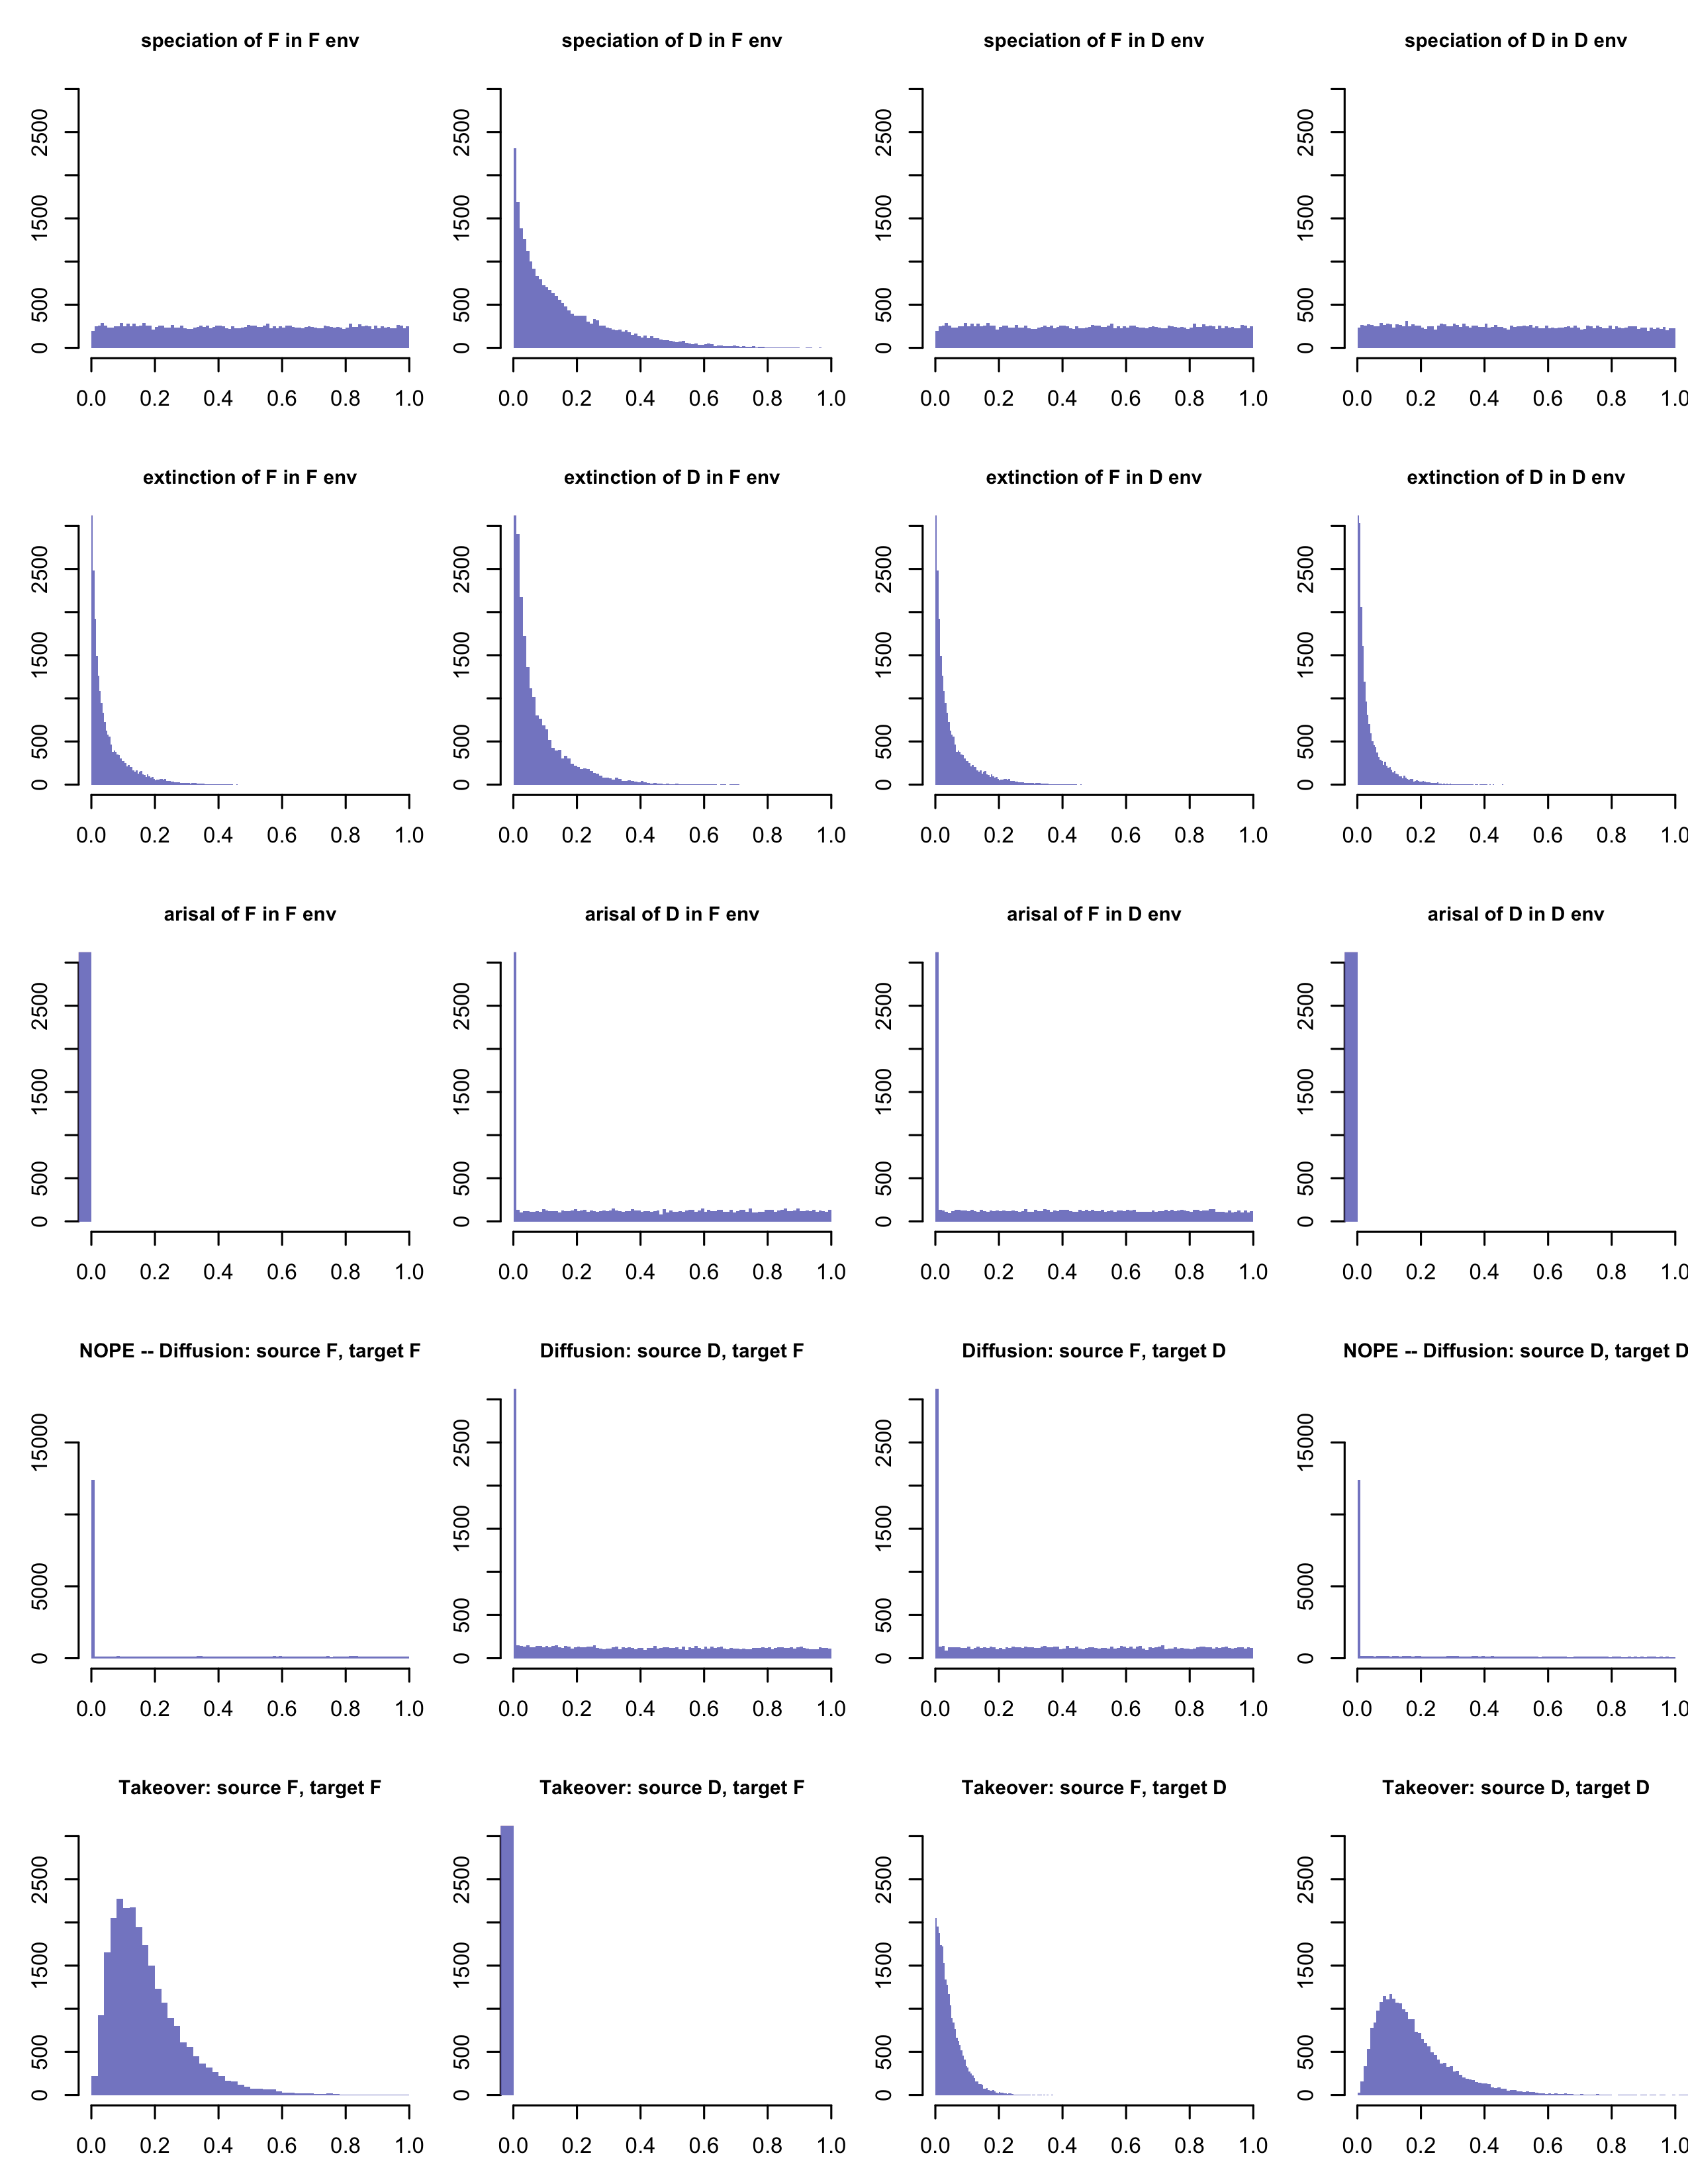
\includegraphics{Global_success_rate_per_parameter.png}
\caption{}
\end{figure}

\section{Random Forest Analysis}\label{random-forest-analysis}

\subsection{Training/Building}\label{trainingbuilding}

The procedures described so far have outlined the creation of a dataset
that includes the input and output variables for each replicate
simulation. When taken as a whole, that dataset describes a distribution
of possible numerical outcomes that are possible given the 4 available
input types. The purpose of the random forest machine learning algorithm
(Breiman 2001, Liaw and Wiener 2015) was to correlate input and output
variables as a means of categorizing simulation outputs according to the
type of input that had created them. We used 70\% of our available
simulation data to build the random forest, the remaining 30\% to test
the forest's accuracy and precision at inferring input categories, and
then used that trained and vetted algorithm to infer the most likely
input category for real world human output data.

This random forest model was trained by building a forest of decision
trees. Each decision tree describes a series of ordered dichotomous
decisions that categorize the 12 output statistics into one of 4 input
types. Individual trees were built by first taking a randomly sized and
randomly selected sample of rows (replicate simulations) and columns
(output variables) from the full simulation dataset to create a unique
subset dataset. That unique dataset was then subjected to a bagging
model to rank the variables in order of importance and build a decision
tree off of that rank. We repeated this process, with replacement, to
build 3000 individual decision trees sampled from 70\% (n = 40000 x 0.7
= 28000) of the total simulation data.

\subsection{Testing}\label{testing}

The random forest was vetted using the remaining 30\% of the simulation
data reserved for model testing. Rather than building decision trees
with these data, we fed each replicate through the recently built forest
so it could classify outputs and then compare those inferred input types
to the known input types to the to see how frequently the forest
returned the correct classification. The accuracy and precision of these
tests are reported in a confusion matrix showing the number of matches
that were correctly or incorrectly made between inputs and outputs for
each model . Our trained random forest algorithm could correctly match
output statistics with input mechanisms with very good accuracy . It is
noteworthy that there was very little confusion between the two
competing hypothesized mechanisms, diffusion and diffusion by takeover.
If the trained random forest algorithm is presented with a simulation
created by diffusion, if is very unlikely to be classify it as coming
from diffusion by takeover.

\subsection{Matching}\label{matching}

The structure of our simulation outputs where designed to mimic the
structure of our real cultural data so that the two could be compared
directly. In the same way the output for replicate simulations where
processed, the phylogeny and spatial pattern of extant human cultures
were summarized using 12 summary statistics passed to the trained random
forest algorithm. The random forest assigned the most likely mechanism
to have caused that human's known historical trajectory. It does this by
asking every dichotomous decision tree in the random forest to vote on
which hypothesized mechanism created the output provided by the data and
then tallying those votes into a consensus vote. Our consensus vote
showed that over 50\% of the trees believe that the current
configuration of agriculture across the globe is the result of demic
diffusion augmented by cultural diffusion. About 35\% of the trees
assigned known global trend to the basic model that includes only demic
diffusion, while the other two models received almost no votes. This
suggest that if we are wrong that demic and cultural diffusion
contributed to current distributions of agriculturist cultures, the next
most likely answer is that it diffusion created these patterns with no
help from cultural diffusion.

\section{Run a single random forest on available
outputs}\label{run-a-single-random-forest-on-available-outputs}

\begin{Shaded}
\begin{Highlighting}[]
\CommentTok{# Packages}
\KeywordTok{library}\NormalTok{(randomForest)}

\CommentTok{# Radom Forest Function}
\NormalTok{RF <-}\StringTok{ }\ControlFlowTok{function}\NormalTok{(table_sim, table_real, }\DataTypeTok{ntree =} \DecValTok{2000}\NormalTok{, }\DataTypeTok{stats_remove =} \OtherTok{NULL}\NormalTok{,}
              \DataTypeTok{repetitions =} \DecValTok{100}\NormalTok{) \{}
 \CommentTok{# table_sim = table croped }

\NormalTok{ begin <-}\StringTok{ }\KeywordTok{which}\NormalTok{(}\KeywordTok{colnames}\NormalTok{(table_sim) }\OperatorTok{==}\StringTok{  "number_of_branches"}\NormalTok{)}
\NormalTok{ table_sim_data <-}\StringTok{ }\NormalTok{table_sim[, begin}\OperatorTok{:}\KeywordTok{ncol}\NormalTok{(table_sim)]}
\NormalTok{ table_sim_data <-}\StringTok{ }\KeywordTok{apply}\NormalTok{(table_sim_data, }\DecValTok{2}\NormalTok{, as.numeric)}
 \ControlFlowTok{if}\NormalTok{ (}\KeywordTok{any}\NormalTok{(}\KeywordTok{is.infinite}\NormalTok{(table_sim_data))) \{}
   \KeywordTok{stop}\NormalTok{(}\StringTok{"There is infinite values in the simulation statistics"}\NormalTok{)}
\NormalTok{ \}}
\NormalTok{ rf_data <-}\StringTok{ }\KeywordTok{data.frame}\NormalTok{(}\StringTok{"Model"}\NormalTok{ =}\StringTok{ }\NormalTok{table_sim}\OperatorTok{$}\NormalTok{combo, table_sim_data)}
\NormalTok{ rf_data_real <-}\StringTok{ }\KeywordTok{data.frame}\NormalTok{(table_real)}

 \ControlFlowTok{if}\NormalTok{ (}\OperatorTok{!}\KeywordTok{is.null}\NormalTok{(stats_remove)) \{}
\NormalTok{   rf_data <-}\StringTok{ }\NormalTok{rf_data[, }\OperatorTok{-}\NormalTok{stats_remove]}
\NormalTok{   rf_data_real <-}\StringTok{ }\NormalTok{rf_data_real[, }\OperatorTok{-}\NormalTok{stats_remove]}
\NormalTok{ \}}

\NormalTok{ fun <-}\StringTok{ }\ControlFlowTok{function}\NormalTok{(x, y, }\DataTypeTok{per =}\NormalTok{ .}\DecValTok{33}\NormalTok{) \{}
   \KeywordTok{sample}\NormalTok{(}\KeywordTok{which}\NormalTok{(y}\OperatorTok{$}\NormalTok{Model }\OperatorTok{==}\StringTok{ }\NormalTok{x), }\KeywordTok{round}\NormalTok{(}\KeywordTok{table}\NormalTok{(y}\OperatorTok{$}\NormalTok{Model)[}\DecValTok{1}\NormalTok{]}\OperatorTok{*}\NormalTok{per))}
\NormalTok{ \}}

\NormalTok{ results <-}\StringTok{ }\KeywordTok{matrix}\NormalTok{(}\DataTypeTok{nrow =}\NormalTok{ repetitions, }\DataTypeTok{ncol =} \KeywordTok{length}\NormalTok{(table_real) }\OperatorTok{*}\StringTok{ }\DecValTok{6} \OperatorTok{+}\StringTok{ }\DecValTok{21}\NormalTok{)}
 \ControlFlowTok{for}\NormalTok{ (i }\ControlFlowTok{in} \DecValTok{1}\OperatorTok{:}\NormalTok{repetitions) \{}
\NormalTok{   sub.test <-}\StringTok{ }\KeywordTok{unlist}\NormalTok{(}\KeywordTok{lapply}\NormalTok{(}\KeywordTok{as.list}\NormalTok{(}\KeywordTok{paste0}\NormalTok{(}\DecValTok{0}\NormalTok{, }\KeywordTok{c}\NormalTok{(}\DecValTok{1}\NormalTok{,}\DecValTok{2}\NormalTok{,}\DecValTok{5}\NormalTok{,}\DecValTok{6}\NormalTok{))), fun,}
                             \DataTypeTok{y =}\NormalTok{ rf_data))}
\NormalTok{   test2 <-}\StringTok{ }\NormalTok{rf_data[sub.test, }\DecValTok{2}\OperatorTok{:}\KeywordTok{ncol}\NormalTok{(rf_data)]}
\NormalTok{   test1 <-}\StringTok{ }\NormalTok{rf_data[sub.test, }\DecValTok{1}\NormalTok{]}
\NormalTok{   train <-}\StringTok{ }\NormalTok{rf_data[}\OperatorTok{-}\NormalTok{sub.test, ]}

\NormalTok{   fit <-}\StringTok{ }\KeywordTok{randomForest}\NormalTok{(Model }\OperatorTok{~}\StringTok{ }\NormalTok{., }\DataTypeTok{data =}\NormalTok{ train, }\DataTypeTok{xtest =}\NormalTok{ test2, }
                       \DataTypeTok{ytest =}\NormalTok{ test1, }\DataTypeTok{importance =} \OtherTok{TRUE}\NormalTok{, }
                       \DataTypeTok{ntree =}\NormalTok{ ntree, }\DataTypeTok{keep.forest =} \OtherTok{TRUE}\NormalTok{,}
                       \DataTypeTok{replace =} \OtherTok{TRUE}\NormalTok{)}
  \CommentTok{#dev.new()}
  \CommentTok{#plot(fit)}
\NormalTok{   predictions <-}\StringTok{ }\KeywordTok{predict}\NormalTok{(fit, rf_data_real, }\DataTypeTok{type =} \StringTok{"prob"}\NormalTok{)}
\NormalTok{   var_import <-}\StringTok{ }\KeywordTok{importance}\NormalTok{(fit)}

\NormalTok{   error <-}\StringTok{ }\KeywordTok{mean}\NormalTok{(fit}\OperatorTok{$}\NormalTok{test}\OperatorTok{$}\NormalTok{confusion[, }\DecValTok{5}\NormalTok{])}
\NormalTok{   confusion <-}\StringTok{ }\KeywordTok{as.numeric}\NormalTok{(fit}\OperatorTok{$}\NormalTok{test}\OperatorTok{$}\NormalTok{confusion[, }\DecValTok{1}\OperatorTok{:}\DecValTok{4}\NormalTok{])}
   \KeywordTok{names}\NormalTok{(confusion) <-}\StringTok{ }\KeywordTok{paste0}\NormalTok{(}\StringTok{"Confusion_"}\NormalTok{, }
                              \KeywordTok{rep}\NormalTok{(}\KeywordTok{colnames}\NormalTok{(fit}\OperatorTok{$}\NormalTok{test}\OperatorTok{$}\NormalTok{confusion[, }\DecValTok{1}\OperatorTok{:}\DecValTok{4}\NormalTok{]),}
                                  \DataTypeTok{each =} \DecValTok{4}\NormalTok{),}
                              \KeywordTok{rownames}\NormalTok{(fit}\OperatorTok{$}\NormalTok{test}\OperatorTok{$}\NormalTok{confusion[, }\DecValTok{1}\OperatorTok{:}\DecValTok{4}\NormalTok{]))}
\NormalTok{   predictions_prob <-}\StringTok{ }\KeywordTok{as.numeric}\NormalTok{(predictions)}
   \KeywordTok{names}\NormalTok{(predictions_prob) <-}\StringTok{ }\KeywordTok{paste0}\NormalTok{(}\StringTok{"Prediction_prob"}\NormalTok{, }\KeywordTok{colnames}\NormalTok{(predictions))}
\NormalTok{   var_import_vec <-}\StringTok{ }\KeywordTok{as.numeric}\NormalTok{(var_import)}
   \KeywordTok{names}\NormalTok{(var_import_vec) <-}\StringTok{ }\KeywordTok{paste0}\NormalTok{(}\StringTok{"var_imp_"}\NormalTok{, }
                                   \KeywordTok{rep}\NormalTok{(}\KeywordTok{colnames}\NormalTok{(var_import), }
                                       \DataTypeTok{each =} \KeywordTok{nrow}\NormalTok{(var_import)),}
                                   \StringTok{"_"}\NormalTok{,}
                                   \KeywordTok{rownames}\NormalTok{(var_import))}
\NormalTok{   vec <-}\StringTok{ }\KeywordTok{c}\NormalTok{(error, confusion, predictions_prob, var_import_vec)}
\NormalTok{   results[i, ] <-}\StringTok{ }\NormalTok{vec}
\NormalTok{ \}}
 \KeywordTok{colnames}\NormalTok{(results) <-}\StringTok{ }\KeywordTok{names}\NormalTok{(vec)}
 \KeywordTok{colnames}\NormalTok{(results)[}\DecValTok{1}\NormalTok{] <-}\StringTok{ "Error_test"}
\NormalTok{ results <-}\StringTok{ }\KeywordTok{cbind}\NormalTok{(}\DecValTok{1}\OperatorTok{:}\KeywordTok{nrow}\NormalTok{(results), results)}
 \KeywordTok{colnames}\NormalTok{(results)[}\DecValTok{1}\NormalTok{] <-}\StringTok{ "Replicate"}
 \KeywordTok{return}\NormalTok{(results)}
\NormalTok{\}}

\CommentTok{# Multiple Random Forest}
\NormalTok{RF_mult <-}\StringTok{ }\ControlFlowTok{function}\NormalTok{(table_sim, table_real_mult, }\DataTypeTok{ntree =} \DecValTok{2000}\NormalTok{, }
                   \DataTypeTok{stats_remove =} \OtherTok{NULL}\NormalTok{, }\DataTypeTok{repetitions =} \DecValTok{100}\NormalTok{) \{}
\NormalTok{ n_r <-}\StringTok{ }\KeywordTok{nrow}\NormalTok{(table_real_mult)}
\NormalTok{ n <-}\StringTok{ }\NormalTok{repetitions }\OperatorTok{*}\StringTok{ }\NormalTok{n_r}
\NormalTok{ n_col <-}\StringTok{ }\KeywordTok{ncol}\NormalTok{(table_real_mult) }\OperatorTok{*}\StringTok{ }\DecValTok{6} \OperatorTok{+}\StringTok{ }\DecValTok{22}
\NormalTok{ results <-}\StringTok{ }\KeywordTok{matrix}\NormalTok{(}\DataTypeTok{nrow =}\NormalTok{ n, }\DataTypeTok{ncol =}\NormalTok{ n_col)}
\NormalTok{ x <-}\StringTok{ }\DecValTok{0}
 \ControlFlowTok{for}\NormalTok{ (i }\ControlFlowTok{in} \KeywordTok{seq}\NormalTok{(}\DecValTok{1}\NormalTok{, n, repetitions)) \{}
\NormalTok{   x <-}\StringTok{ }\NormalTok{x }\OperatorTok{+}\StringTok{ }\DecValTok{1}
\NormalTok{   temp <-}\StringTok{ }\KeywordTok{RF}\NormalTok{(table_sim, }
\NormalTok{              table_real_mult[x, , }\DataTypeTok{drop =} \OtherTok{FALSE}\NormalTok{],}
              \DataTypeTok{ntree =}\NormalTok{ ntree, }
              \DataTypeTok{repetitions =}\NormalTok{ repetitions, }
              \DataTypeTok{stats_remove =}\NormalTok{ stats_remove)}
\NormalTok{   results[i}\OperatorTok{:}\NormalTok{(i }\OperatorTok{+}\StringTok{ }\NormalTok{repetitions }\OperatorTok{-}\StringTok{ }\DecValTok{1}\NormalTok{), ] <-}\StringTok{ }\NormalTok{temp}
\NormalTok{ \}}
\NormalTok{ tree <-}\StringTok{ }\KeywordTok{rep}\NormalTok{(}\DecValTok{1}\OperatorTok{:}\NormalTok{n_r, }\DataTypeTok{each =}\NormalTok{ repetitions)}
\NormalTok{ results <-}\StringTok{ }\KeywordTok{cbind}\NormalTok{(tree, results)}
 \KeywordTok{colnames}\NormalTok{(results) <-}\StringTok{ }\KeywordTok{c}\NormalTok{(}\StringTok{"Tree"}\NormalTok{, }\KeywordTok{colnames}\NormalTok{(temp))}
 \KeywordTok{return}\NormalTok{(results)}
\NormalTok{\}}

\CommentTok{# Accumulation function}
\NormalTok{RF_acum <-}\StringTok{ }\ControlFlowTok{function}\NormalTok{(table_sim, table_real_mult, }\DataTypeTok{ntree =} \DecValTok{2000}\NormalTok{, }
                   \DataTypeTok{stats_remove =} \OtherTok{NULL}\NormalTok{, }\DataTypeTok{repetitions =} \DecValTok{100}\NormalTok{,}
                   \DataTypeTok{resolution =} \DecValTok{100}\NormalTok{, }\DataTypeTok{minimun =} \DecValTok{100}\NormalTok{) \{}
\NormalTok{ sequence <-}\StringTok{ }\KeywordTok{seq}\NormalTok{(minimun, }\KeywordTok{nrow}\NormalTok{(table_sim), resolution)}
\NormalTok{ n_col <-}\StringTok{ }\KeywordTok{ncol}\NormalTok{(table_real_mult) }\OperatorTok{*}\StringTok{ }\DecValTok{6} \OperatorTok{+}\StringTok{ }\DecValTok{24} 
\NormalTok{ n_r <-}\StringTok{ }\KeywordTok{nrow}\NormalTok{(table_real_mult)}
\NormalTok{ n_seq <-}\StringTok{ }\KeywordTok{length}\NormalTok{(sequence)}
\NormalTok{ n <-}\StringTok{ }\NormalTok{repetitions }\OperatorTok{*}\StringTok{ }\NormalTok{n_r }\OperatorTok{*}\StringTok{ }\NormalTok{n_seq}
\NormalTok{ results <-}\StringTok{ }\KeywordTok{matrix}\NormalTok{(}\DataTypeTok{nrow =}\NormalTok{ n, }\DataTypeTok{ncol =}\NormalTok{ n_col)}
\NormalTok{ lottery1 <-}\StringTok{ }\KeywordTok{which}\NormalTok{(table_sim}\OperatorTok{$}\NormalTok{combo }\OperatorTok{==}\StringTok{ "01"}\NormalTok{)}
\NormalTok{ lottery2 <-}\StringTok{ }\KeywordTok{which}\NormalTok{(table_sim}\OperatorTok{$}\NormalTok{combo }\OperatorTok{==}\StringTok{ "02"}\NormalTok{)}
\NormalTok{ lottery5 <-}\StringTok{ }\KeywordTok{which}\NormalTok{(table_sim}\OperatorTok{$}\NormalTok{combo }\OperatorTok{==}\StringTok{ "05"}\NormalTok{)}
\NormalTok{ lottery6 <-}\StringTok{ }\KeywordTok{which}\NormalTok{(table_sim}\OperatorTok{$}\NormalTok{combo }\OperatorTok{==}\StringTok{ "06"}\NormalTok{)}
\NormalTok{ sub1 <-}\StringTok{ }\KeywordTok{sample}\NormalTok{(lottery1, sequence[}\DecValTok{1}\NormalTok{]}\OperatorTok{/}\DecValTok{4}\NormalTok{, }\DataTypeTok{replace =} \OtherTok{FALSE}\NormalTok{)}
\NormalTok{ sub2 <-}\StringTok{ }\KeywordTok{sample}\NormalTok{(lottery2, sequence[}\DecValTok{1}\NormalTok{]}\OperatorTok{/}\DecValTok{4}\NormalTok{, }\DataTypeTok{replace =} \OtherTok{FALSE}\NormalTok{)}
\NormalTok{ sub5 <-}\StringTok{ }\KeywordTok{sample}\NormalTok{(lottery5, sequence[}\DecValTok{1}\NormalTok{]}\OperatorTok{/}\DecValTok{4}\NormalTok{, }\DataTypeTok{replace =} \OtherTok{FALSE}\NormalTok{)}
\NormalTok{ sub6 <-}\StringTok{ }\KeywordTok{sample}\NormalTok{(lottery6, sequence[}\DecValTok{1}\NormalTok{]}\OperatorTok{/}\DecValTok{4}\NormalTok{, }\DataTypeTok{replace =} \OtherTok{FALSE}\NormalTok{)}
 \ControlFlowTok{for}\NormalTok{ (i }\ControlFlowTok{in} \DecValTok{1}\OperatorTok{:}\NormalTok{n_seq) \{}
   \ControlFlowTok{if}\NormalTok{ (i }\OperatorTok{!=}\StringTok{ }\DecValTok{1}\NormalTok{) \{}
\NormalTok{     sub1 <-}\StringTok{ }\KeywordTok{c}\NormalTok{(sub1, }\KeywordTok{sample}\NormalTok{(lottery1[}\OperatorTok{-}\NormalTok{sub1], sequence[}\DecValTok{1}\NormalTok{]}\OperatorTok{/}\DecValTok{4}\NormalTok{, }\DataTypeTok{replace =} \OtherTok{FALSE}\NormalTok{))}
\NormalTok{     sub2 <-}\StringTok{ }\KeywordTok{c}\NormalTok{(sub2, }\KeywordTok{sample}\NormalTok{(lottery2[}\OperatorTok{-}\NormalTok{sub2], sequence[}\DecValTok{1}\NormalTok{]}\OperatorTok{/}\DecValTok{4}\NormalTok{, }\DataTypeTok{replace =} \OtherTok{FALSE}\NormalTok{))}
\NormalTok{     sub5 <-}\StringTok{ }\KeywordTok{c}\NormalTok{(sub5, }\KeywordTok{sample}\NormalTok{(lottery5[}\OperatorTok{-}\NormalTok{sub5], sequence[}\DecValTok{1}\NormalTok{]}\OperatorTok{/}\DecValTok{4}\NormalTok{, }\DataTypeTok{replace =} \OtherTok{FALSE}\NormalTok{))}
\NormalTok{     sub6 <-}\StringTok{ }\KeywordTok{c}\NormalTok{(sub6, }\KeywordTok{sample}\NormalTok{(lottery6[}\OperatorTok{-}\NormalTok{sub6], sequence[}\DecValTok{1}\NormalTok{]}\OperatorTok{/}\DecValTok{4}\NormalTok{, }\DataTypeTok{replace =} \OtherTok{FALSE}\NormalTok{))}
\NormalTok{   \}}
\NormalTok{   temp <-}\StringTok{ }\KeywordTok{RF_mult}\NormalTok{(table_sim[}\KeywordTok{c}\NormalTok{(sub1, sub2, sub5, sub6), ], table_real_mult,}
                   \DataTypeTok{ntree =}\NormalTok{ ntree, }\DataTypeTok{repetitions =}\NormalTok{ repetitions,}
                   \DataTypeTok{stats_remove =}\NormalTok{ stats_remove)}
\NormalTok{   n_temp <-}\StringTok{ }\KeywordTok{nrow}\NormalTok{(temp)}
\NormalTok{   results[}\DecValTok{1}\OperatorTok{:}\NormalTok{n_temp }\OperatorTok{+}\StringTok{ }\NormalTok{(n_temp }\OperatorTok{*}\StringTok{ }\NormalTok{(i }\OperatorTok{-}\StringTok{ }\DecValTok{1}\NormalTok{)), ] <-}\StringTok{ }\KeywordTok{cbind}\NormalTok{(}\KeywordTok{rep}\NormalTok{(sequence[i],}
\NormalTok{                                                         n_temp), temp)}
\NormalTok{ \}}
 \KeywordTok{colnames}\NormalTok{(results) <-}\StringTok{ }\KeywordTok{c}\NormalTok{(}\StringTok{"Subsample_size"}\NormalTok{, }\KeywordTok{colnames}\NormalTok{(temp))}
 \KeywordTok{return}\NormalTok{(results)}
\NormalTok{\}}

\CommentTok{# }\AlertTok{TEST}\CommentTok{ FINAL (RUN ONLY THIS)}
\CommentTok{# Load data}
\KeywordTok{setwd}\NormalTok{(}\StringTok{"~/Desktop/RF after bruno"}\NormalTok{)}
\KeywordTok{load}\NormalTok{(}\StringTok{"Four model compare third runFour_model_compare_results_28_Jul_2017_crop_to_5767.Rdata"}\NormalTok{)}
\KeywordTok{load}\NormalTok{(}\StringTok{"real.analysis_mult.RData"}\NormalTok{)}

\NormalTok{table_sim =}\StringTok{ }\NormalTok{Concatenated_data}
\NormalTok{table_real =}\StringTok{ }\NormalTok{real.analysis.mult[[}\DecValTok{1}\NormalTok{]][[}\DecValTok{1}\NormalTok{]]}
\NormalTok{table_real_mult =}\StringTok{ }\KeywordTok{do.call}\NormalTok{(rbind, }\KeywordTok{lapply}\NormalTok{(real.analysis.mult, }
                                       \ControlFlowTok{function}\NormalTok{(x)\{x[[}\DecValTok{1}\NormalTok{]]\}))}

\CommentTok{#start time}
\NormalTok{time_start <-}\StringTok{ }\KeywordTok{Sys.time}\NormalTok{()}

\CommentTok{# Change the parameters as you wish}
\NormalTok{res_acum <-}\StringTok{ }\KeywordTok{RF_acum}\NormalTok{(table_sim, table_real_mult[}\DecValTok{100}\OperatorTok{:}\DecValTok{110}\NormalTok{,,}\DataTypeTok{drop=}\OtherTok{FALSE}\NormalTok{], }\DataTypeTok{ntree =} \DecValTok{2000}\NormalTok{, }
                   \DataTypeTok{stats_remove =} \OtherTok{NULL}\NormalTok{, }\DataTypeTok{repetitions =} \DecValTok{1}\NormalTok{,}
                   \DataTypeTok{resolution =} \DecValTok{5000}\NormalTok{, }\DataTypeTok{minimun =} \DecValTok{1000}\NormalTok{)}
                   
\CommentTok{#stop time}
\NormalTok{time_stop <-}\StringTok{ }\KeywordTok{Sys.time}\NormalTok{()}
\KeywordTok{difftime}\NormalTok{(time_stop, time_start)                   }

\KeywordTok{save}\NormalTok{(res_acum, }\DataTypeTok{file=}\StringTok{"~/Desktop/10_more_tree_out.Rdata"}\NormalTok{)}

\CommentTok{# Change argument FUN to sd to obtain the standard deviation}
\KeywordTok{plot}\NormalTok{(}\KeywordTok{aggregate}\NormalTok{(}\DataTypeTok{x =}\NormalTok{ res_acum[, }\DecValTok{4}\NormalTok{], }\DataTypeTok{by =} \KeywordTok{list}\NormalTok{((res_acum[, }\DecValTok{1}\NormalTok{])), }\DataTypeTok{FUN =}\NormalTok{ mean), }\DataTypeTok{type =} \StringTok{"n"}\NormalTok{, }\DataTypeTok{ylim=}\KeywordTok{c}\NormalTok{(}\DecValTok{0}\NormalTok{,}\DecValTok{1}\NormalTok{))}

\KeywordTok{lines}\NormalTok{(}\KeywordTok{aggregate}\NormalTok{(}\DataTypeTok{x =}\NormalTok{ res_acum[, }\DecValTok{21}\NormalTok{], }\DataTypeTok{by =} \KeywordTok{list}\NormalTok{((res_acum[, }\DecValTok{1}\NormalTok{])), }\DataTypeTok{FUN =}\NormalTok{ mean), }\DataTypeTok{type =} \StringTok{"l"}\NormalTok{, }\DataTypeTok{col=}\StringTok{"orange"}\NormalTok{)}
\KeywordTok{lines}\NormalTok{(}\KeywordTok{aggregate}\NormalTok{(}\DataTypeTok{x =}\NormalTok{ res_acum[, }\DecValTok{22}\NormalTok{], }\DataTypeTok{by =} \KeywordTok{list}\NormalTok{((res_acum[, }\DecValTok{1}\NormalTok{])), }\DataTypeTok{FUN =}\NormalTok{ mean), }\DataTypeTok{type =} \StringTok{"l"}\NormalTok{, }\DataTypeTok{col=}\StringTok{"blue"}\NormalTok{)}
\KeywordTok{lines}\NormalTok{(}\KeywordTok{aggregate}\NormalTok{(}\DataTypeTok{x =}\NormalTok{ res_acum[, }\DecValTok{23}\NormalTok{], }\DataTypeTok{by =} \KeywordTok{list}\NormalTok{((res_acum[, }\DecValTok{1}\NormalTok{])), }\DataTypeTok{FUN =}\NormalTok{ mean), }\DataTypeTok{type =} \StringTok{"l"}\NormalTok{, }\DataTypeTok{col=}\StringTok{"pink"}\NormalTok{)}
\KeywordTok{lines}\NormalTok{(}\KeywordTok{aggregate}\NormalTok{(}\DataTypeTok{x =}\NormalTok{ res_acum[, }\DecValTok{24}\NormalTok{], }\DataTypeTok{by =} \KeywordTok{list}\NormalTok{((res_acum[, }\DecValTok{1}\NormalTok{])), }\DataTypeTok{FUN =}\NormalTok{ mean), }\DataTypeTok{type =} \StringTok{"l"}\NormalTok{, }\DataTypeTok{col=}\StringTok{"darkgreen"}\NormalTok{)}
\end{Highlighting}
\end{Shaded}

\section{Visualize outputs from Random Forest
analysis}\label{visualize-outputs-from-random-forest-analysis}

\begin{Shaded}
\begin{Highlighting}[]
\CommentTok{# load outputs from RF runs}
\KeywordTok{load}\NormalTok{(}\StringTok{"/Users/Ty/Desktop/small_RF_out.Rdata"}\NormalTok{)}
\NormalTok{a <-}\StringTok{ }\NormalTok{res_acum}

\KeywordTok{load}\NormalTok{(}\StringTok{"/Users/Ty/Desktop/10_more_tree_out.Rdata"}\NormalTok{)}
\NormalTok{b <-}\StringTok{ }\NormalTok{res_acum}

\KeywordTok{load}\NormalTok{(}\StringTok{"/Users/Ty/Desktop/10_tree_out.Rdata"}\NormalTok{)}
\NormalTok{c <-}\StringTok{ }\NormalTok{res_acum}

\CommentTok{#object called res_acum}
\NormalTok{res_acum <-}\StringTok{ }\KeywordTok{rbind}\NormalTok{(b,c)}

\KeywordTok{load}\NormalTok{(}\StringTok{"Random_Forest_output_data_for_publication_2_February_2018.Rdata"}\NormalTok{)}
\end{Highlighting}
\end{Shaded}

\begin{Shaded}
\begin{Highlighting}[]
\KeywordTok{png}\NormalTok{(}\StringTok{"overall_error_per_sample_size.png"}\NormalTok{, }\DataTypeTok{width =} \DecValTok{11}\NormalTok{, }\DataTypeTok{height =} \FloatTok{8.5}\NormalTok{, }\DataTypeTok{res =} \DecValTok{300}\NormalTok{, }\DataTypeTok{units =} \StringTok{"in"}\NormalTok{)}
\KeywordTok{plot}\NormalTok{(}\KeywordTok{aggregate}\NormalTok{(}\DataTypeTok{x =}\NormalTok{ res_acum[, }\DecValTok{4}\NormalTok{], }\DataTypeTok{by =} \KeywordTok{list}\NormalTok{((res_acum[, }\DecValTok{1}\NormalTok{])), }\DataTypeTok{FUN =}\NormalTok{ mean), }\DataTypeTok{type=}\StringTok{"l"}\NormalTok{, }\DataTypeTok{ylim=}\KeywordTok{c}\NormalTok{(}\DecValTok{0}\NormalTok{,}\FloatTok{0.5}\NormalTok{), }\DataTypeTok{ylab=}\StringTok{"overall confusion error"}\NormalTok{, }\DataTypeTok{xlab=}\StringTok{"sample size"}\NormalTok{)}
\KeywordTok{dev.off}\NormalTok{()}
\end{Highlighting}
\end{Shaded}

\begin{figure}
\centering
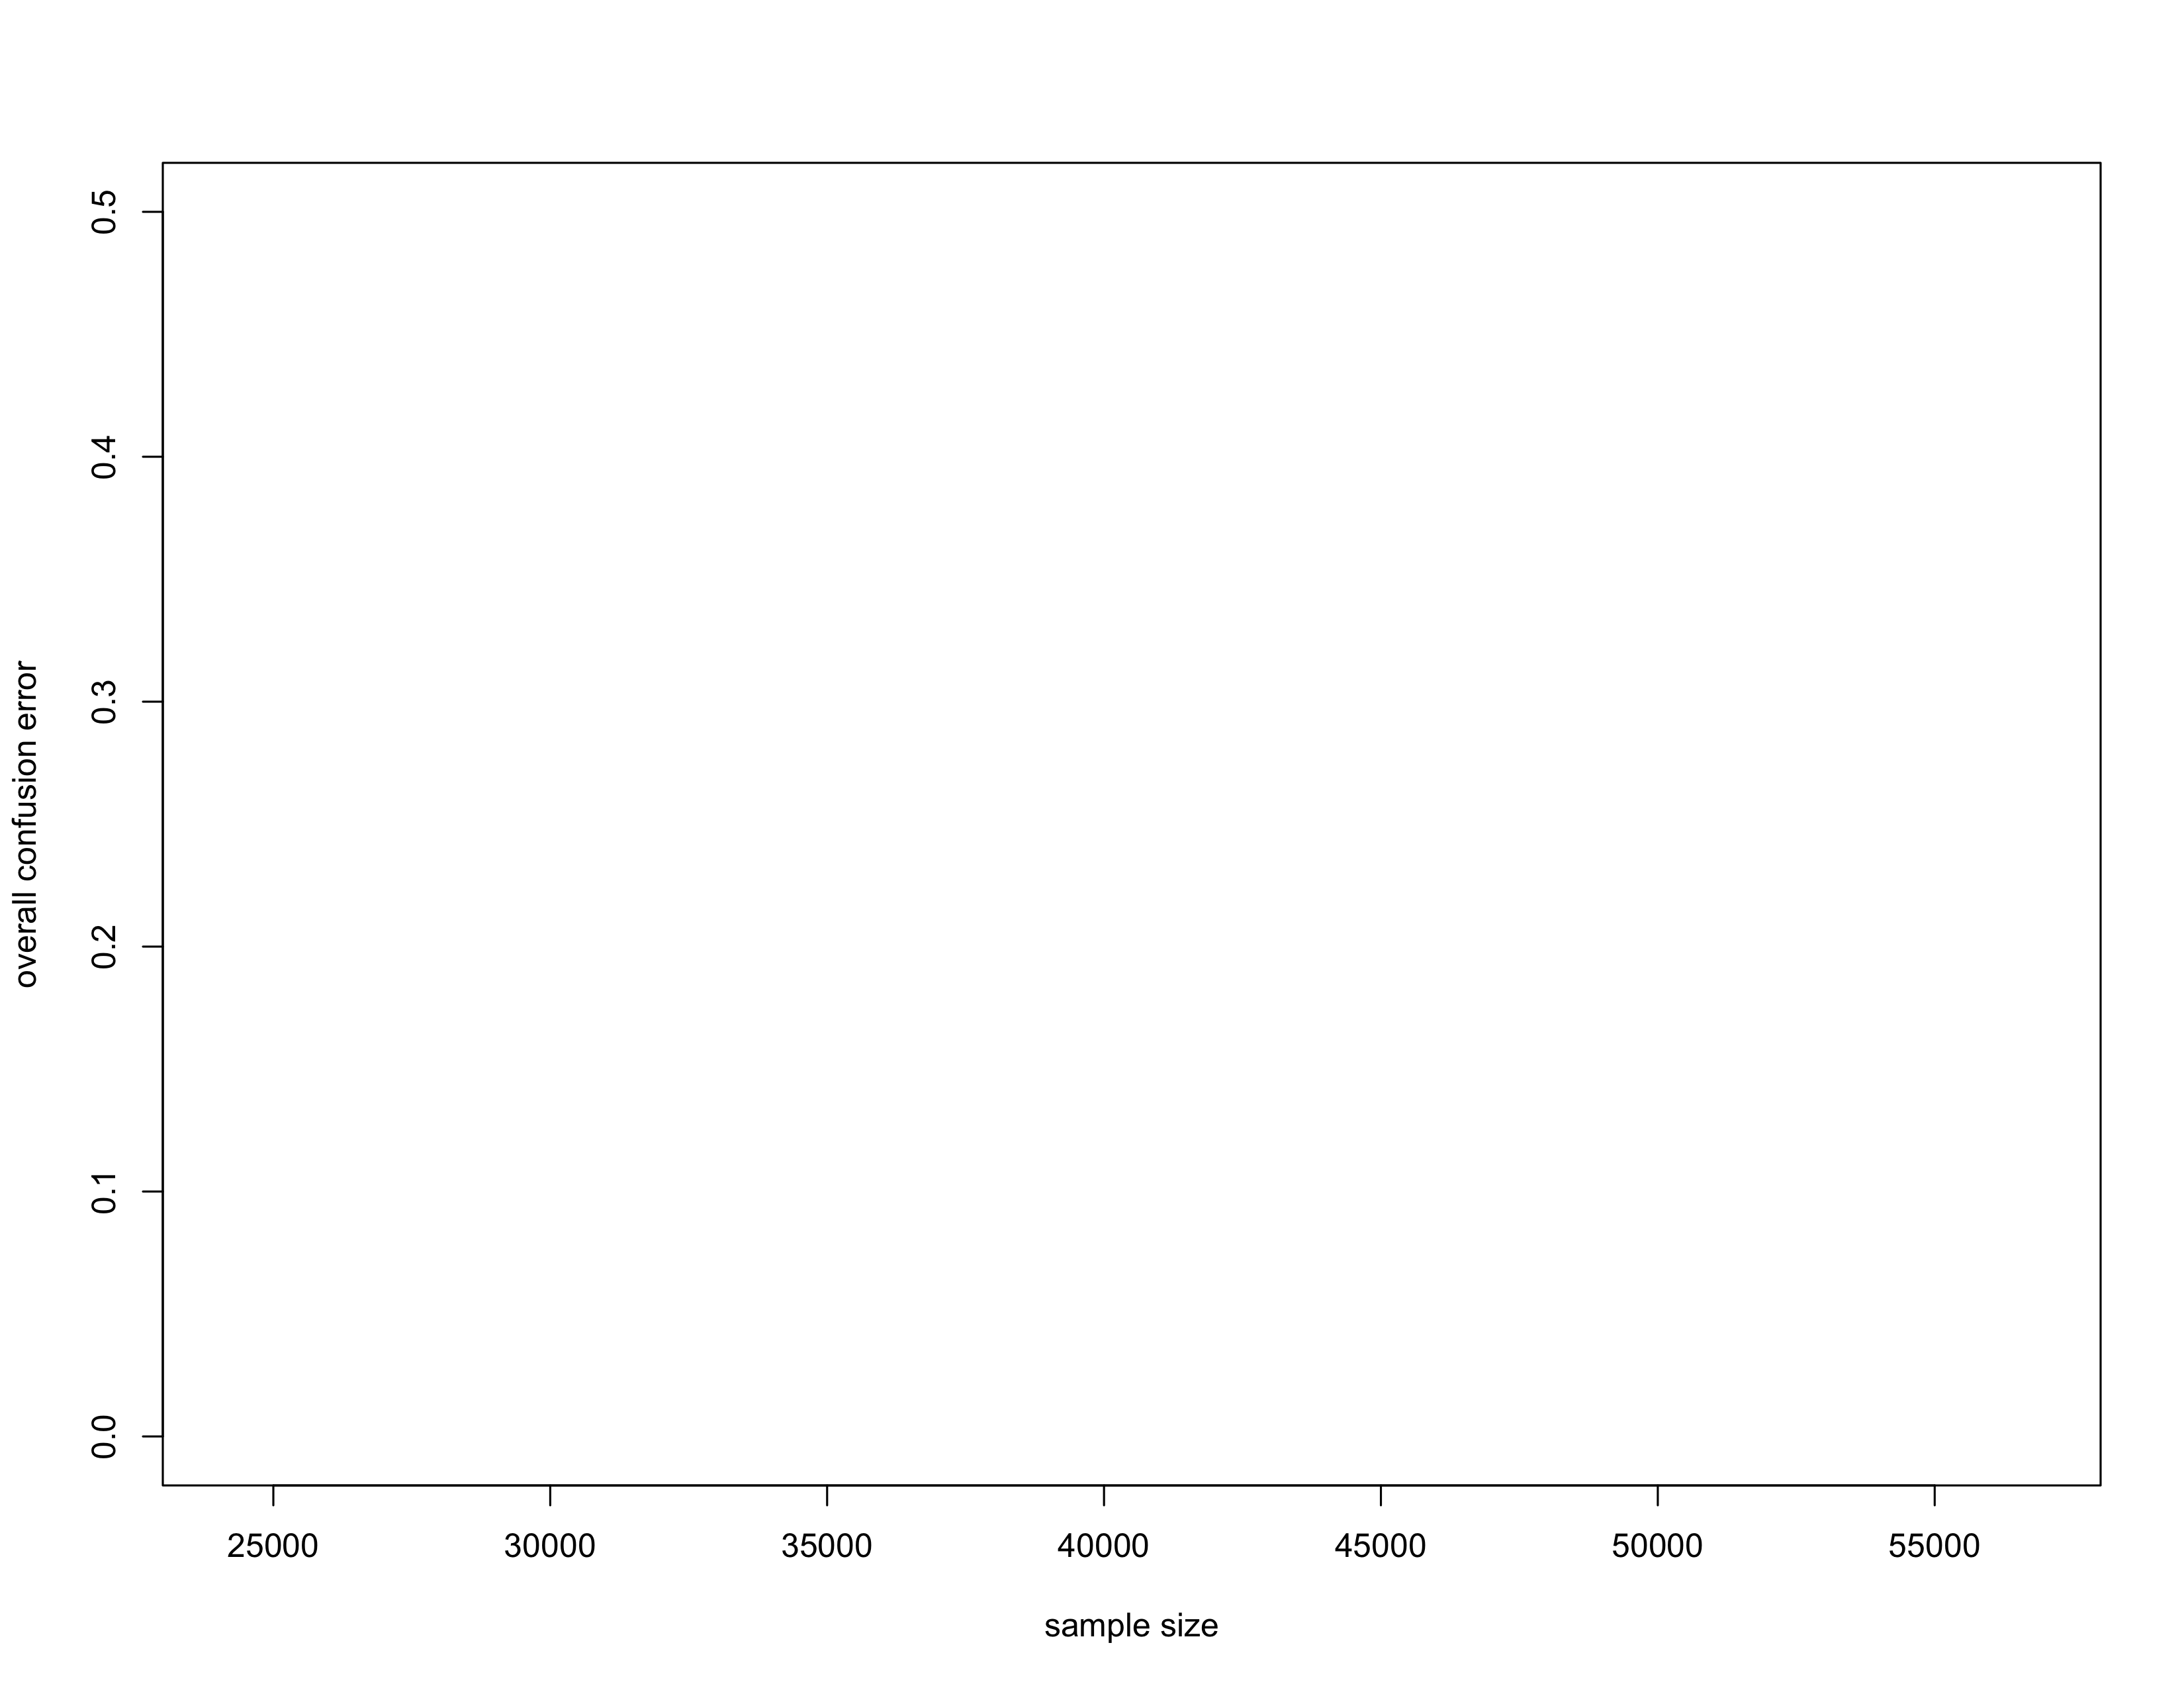
\includegraphics{overall_error_per_sample_size.png}
\caption{}
\end{figure}

\begin{Shaded}
\begin{Highlighting}[]
\KeywordTok{png}\NormalTok{(}\StringTok{"predictions.png"}\NormalTok{, }\DataTypeTok{width =} \DecValTok{11}\NormalTok{, }\DataTypeTok{height =} \FloatTok{8.5}\NormalTok{, }\DataTypeTok{res =} \DecValTok{300}\NormalTok{, }\DataTypeTok{units =} \StringTok{"in"}\NormalTok{)}
\KeywordTok{par}\NormalTok{(}\DataTypeTok{mar=}\KeywordTok{c}\NormalTok{(}\DecValTok{5}\NormalTok{,}\DecValTok{6}\NormalTok{,}\DecValTok{2}\NormalTok{,}\DecValTok{1}\NormalTok{))}

\CommentTok{# Change argument FUN to sd to obtain the standard deviation}
\KeywordTok{plot}\NormalTok{(}\KeywordTok{aggregate}\NormalTok{(}\DataTypeTok{x =}\NormalTok{ res_acum[, }\DecValTok{4}\NormalTok{], }\DataTypeTok{by =} \KeywordTok{list}\NormalTok{((res_acum[, }\DecValTok{1}\NormalTok{])), }\DataTypeTok{FUN =}\NormalTok{ mean), }\DataTypeTok{type =} \StringTok{"n"}\NormalTok{, }\DataTypeTok{ylim=}\KeywordTok{c}\NormalTok{(}\DecValTok{0}\NormalTok{,}\DecValTok{1}\NormalTok{), }\DataTypeTok{ylab=}\StringTok{"probability that our known cultural phylogeny came }\CharTok{\textbackslash{}n}\StringTok{ from each type of simulated mechanism"}\NormalTok{, }\DataTypeTok{xlab=}\StringTok{"number of simulation replicates"}\NormalTok{, }\DataTypeTok{cex.axis=}\FloatTok{1.5}\NormalTok{, }\DataTypeTok{cex.lab=}\FloatTok{1.5}\NormalTok{)}


\NormalTok{basic_mean <-}\StringTok{ }\KeywordTok{aggregate}\NormalTok{(}\DataTypeTok{x =}\NormalTok{ res_acum[, }\DecValTok{21}\NormalTok{], }\DataTypeTok{by =} \KeywordTok{list}\NormalTok{((res_acum[, }\DecValTok{1}\NormalTok{])), }\DataTypeTok{FUN =}\NormalTok{ mean)}
\NormalTok{diffusion_mean <-}\StringTok{ }\KeywordTok{aggregate}\NormalTok{(}\DataTypeTok{x =}\NormalTok{ res_acum[, }\DecValTok{22}\NormalTok{], }\DataTypeTok{by =} \KeywordTok{list}\NormalTok{((res_acum[, }\DecValTok{1}\NormalTok{])), }\DataTypeTok{FUN =}\NormalTok{ mean)}
\NormalTok{TO_mean <-}\StringTok{ }\KeywordTok{aggregate}\NormalTok{(}\DataTypeTok{x =}\NormalTok{ res_acum[, }\DecValTok{23}\NormalTok{], }\DataTypeTok{by =} \KeywordTok{list}\NormalTok{((res_acum[, }\DecValTok{1}\NormalTok{])), }\DataTypeTok{FUN =}\NormalTok{ mean)}
\NormalTok{both_mean <-}\StringTok{ }\KeywordTok{aggregate}\NormalTok{(}\DataTypeTok{x =}\NormalTok{ res_acum[, }\DecValTok{24}\NormalTok{], }\DataTypeTok{by =} \KeywordTok{list}\NormalTok{((res_acum[, }\DecValTok{1}\NormalTok{])), }\DataTypeTok{FUN =}\NormalTok{ mean)}
                   
\NormalTok{basic_sd <-}\StringTok{ }\KeywordTok{aggregate}\NormalTok{(}\DataTypeTok{x =}\NormalTok{ res_acum[, }\DecValTok{21}\NormalTok{], }\DataTypeTok{by =} \KeywordTok{list}\NormalTok{((res_acum[, }\DecValTok{1}\NormalTok{])), }\DataTypeTok{FUN =}\NormalTok{ sd)}
\NormalTok{diffusion_sd <-}\StringTok{ }\KeywordTok{aggregate}\NormalTok{(}\DataTypeTok{x =}\NormalTok{ res_acum[, }\DecValTok{22}\NormalTok{], }\DataTypeTok{by =} \KeywordTok{list}\NormalTok{((res_acum[, }\DecValTok{1}\NormalTok{])), }\DataTypeTok{FUN =}\NormalTok{ sd)}
\NormalTok{TO_sd <-}\StringTok{ }\KeywordTok{aggregate}\NormalTok{(}\DataTypeTok{x =}\NormalTok{ res_acum[, }\DecValTok{23}\NormalTok{], }\DataTypeTok{by =} \KeywordTok{list}\NormalTok{((res_acum[, }\DecValTok{1}\NormalTok{])), }\DataTypeTok{FUN =}\NormalTok{ sd)}
\NormalTok{both_sd <-}\StringTok{ }\KeywordTok{aggregate}\NormalTok{(}\DataTypeTok{x =}\NormalTok{ res_acum[, }\DecValTok{24}\NormalTok{], }\DataTypeTok{by =} \KeywordTok{list}\NormalTok{((res_acum[, }\DecValTok{1}\NormalTok{])), }\DataTypeTok{FUN =}\NormalTok{ sd)}


\KeywordTok{polygon}\NormalTok{(}\DataTypeTok{x=}\KeywordTok{c}\NormalTok{(basic_mean[,}\DecValTok{1}\NormalTok{], }\KeywordTok{rev}\NormalTok{(basic_mean[,}\DecValTok{1}\NormalTok{])), }\DataTypeTok{y=}\KeywordTok{c}\NormalTok{(basic_mean[,}\DecValTok{2}\NormalTok{] }\OperatorTok{+}\StringTok{ }\NormalTok{basic_sd[,}\DecValTok{2}\NormalTok{], }\KeywordTok{rev}\NormalTok{(basic_mean[,}\DecValTok{2}\NormalTok{] }\OperatorTok{-}\StringTok{ }\NormalTok{basic_sd[,}\DecValTok{2}\NormalTok{])), }\DataTypeTok{col=}\KeywordTok{adjustcolor}\NormalTok{(}\StringTok{"orange"}\NormalTok{, }\DataTypeTok{alpha=}\FloatTok{0.5}\NormalTok{), }\DataTypeTok{border=}\OtherTok{NA}\NormalTok{)}
\KeywordTok{polygon}\NormalTok{(}\DataTypeTok{x=}\KeywordTok{c}\NormalTok{(diffusion_mean[,}\DecValTok{1}\NormalTok{], }\KeywordTok{rev}\NormalTok{(diffusion_mean[,}\DecValTok{1}\NormalTok{])), }\DataTypeTok{y=}\KeywordTok{c}\NormalTok{(diffusion_mean[,}\DecValTok{2}\NormalTok{] }\OperatorTok{+}\StringTok{ }\NormalTok{diffusion_sd[,}\DecValTok{2}\NormalTok{], }\KeywordTok{rev}\NormalTok{(diffusion_mean[,}\DecValTok{2}\NormalTok{] }\OperatorTok{-}\StringTok{ }\NormalTok{diffusion_sd[,}\DecValTok{2}\NormalTok{])), }\DataTypeTok{col=}\KeywordTok{adjustcolor}\NormalTok{(}\StringTok{"cornflowerblue"}\NormalTok{, }\DataTypeTok{alpha=}\FloatTok{0.5}\NormalTok{), }\DataTypeTok{border=}\OtherTok{NA}\NormalTok{)}
\KeywordTok{polygon}\NormalTok{(}\DataTypeTok{x=}\KeywordTok{c}\NormalTok{(TO_mean[,}\DecValTok{1}\NormalTok{], }\KeywordTok{rev}\NormalTok{(TO_mean[,}\DecValTok{1}\NormalTok{])), }\DataTypeTok{y=}\KeywordTok{c}\NormalTok{(TO_mean[,}\DecValTok{2}\NormalTok{] }\OperatorTok{+}\StringTok{ }\NormalTok{TO_sd[,}\DecValTok{2}\NormalTok{], }\KeywordTok{rev}\NormalTok{(TO_mean[,}\DecValTok{2}\NormalTok{] }\OperatorTok{-}\StringTok{ }\NormalTok{TO_sd[,}\DecValTok{2}\NormalTok{])), }\DataTypeTok{col=}\KeywordTok{adjustcolor}\NormalTok{(}\StringTok{"pink"}\NormalTok{, }\DataTypeTok{alpha=}\FloatTok{0.5}\NormalTok{), }\DataTypeTok{border=}\OtherTok{NA}\NormalTok{)}
\KeywordTok{polygon}\NormalTok{(}\DataTypeTok{x=}\KeywordTok{c}\NormalTok{(both_mean[,}\DecValTok{1}\NormalTok{], }\KeywordTok{rev}\NormalTok{(both_mean[,}\DecValTok{1}\NormalTok{])), }\DataTypeTok{y=}\KeywordTok{c}\NormalTok{(both_mean[,}\DecValTok{2}\NormalTok{] }\OperatorTok{+}\StringTok{ }\NormalTok{both_sd[,}\DecValTok{2}\NormalTok{], }\KeywordTok{rev}\NormalTok{(both_mean[,}\DecValTok{2}\NormalTok{] }\OperatorTok{-}\StringTok{ }\NormalTok{both_sd[,}\DecValTok{2}\NormalTok{])), }\DataTypeTok{col=}\KeywordTok{adjustcolor}\NormalTok{(}\StringTok{"darkgreen"}\NormalTok{, }\DataTypeTok{alpha=}\FloatTok{0.5}\NormalTok{), }\DataTypeTok{border=}\OtherTok{NA}\NormalTok{)}



\KeywordTok{lines}\NormalTok{(basic_mean,  }\DataTypeTok{col=}\StringTok{"orange"}\NormalTok{)}
\KeywordTok{lines}\NormalTok{(diffusion_mean,  }\DataTypeTok{col=}\StringTok{"cornflowerblue"}\NormalTok{)}
\KeywordTok{lines}\NormalTok{(TO_mean,  }\DataTypeTok{col=}\StringTok{"pink"}\NormalTok{)}
\KeywordTok{lines}\NormalTok{(both_mean,  }\DataTypeTok{col=}\StringTok{"darkgreen"}\NormalTok{)}

\NormalTok{labs <-}\StringTok{ }\KeywordTok{c}\NormalTok{(}\StringTok{"Basic"}\NormalTok{, }\StringTok{"+Diffusion"}\NormalTok{, }\StringTok{"+Takeover"}\NormalTok{, }\StringTok{"+Diffusion +Takeover"}\NormalTok{)}
\KeywordTok{legend}\NormalTok{(}\StringTok{"topright"}\NormalTok{, }\DataTypeTok{legend=}\NormalTok{labs, }\DataTypeTok{col=}\KeywordTok{c}\NormalTok{(}\StringTok{"orange"}\NormalTok{, }\StringTok{"cornflowerblue"}\NormalTok{, }\StringTok{"pink"}\NormalTok{, }\StringTok{"darkgreen"}\NormalTok{), }\DataTypeTok{lty=}\DecValTok{1}\NormalTok{, }\DataTypeTok{cex=}\FloatTok{1.5}\NormalTok{, }\DataTypeTok{lwd=}\DecValTok{10}\NormalTok{)}

\KeywordTok{dev.off}\NormalTok{()}
\end{Highlighting}
\end{Shaded}

\begin{figure}
\centering
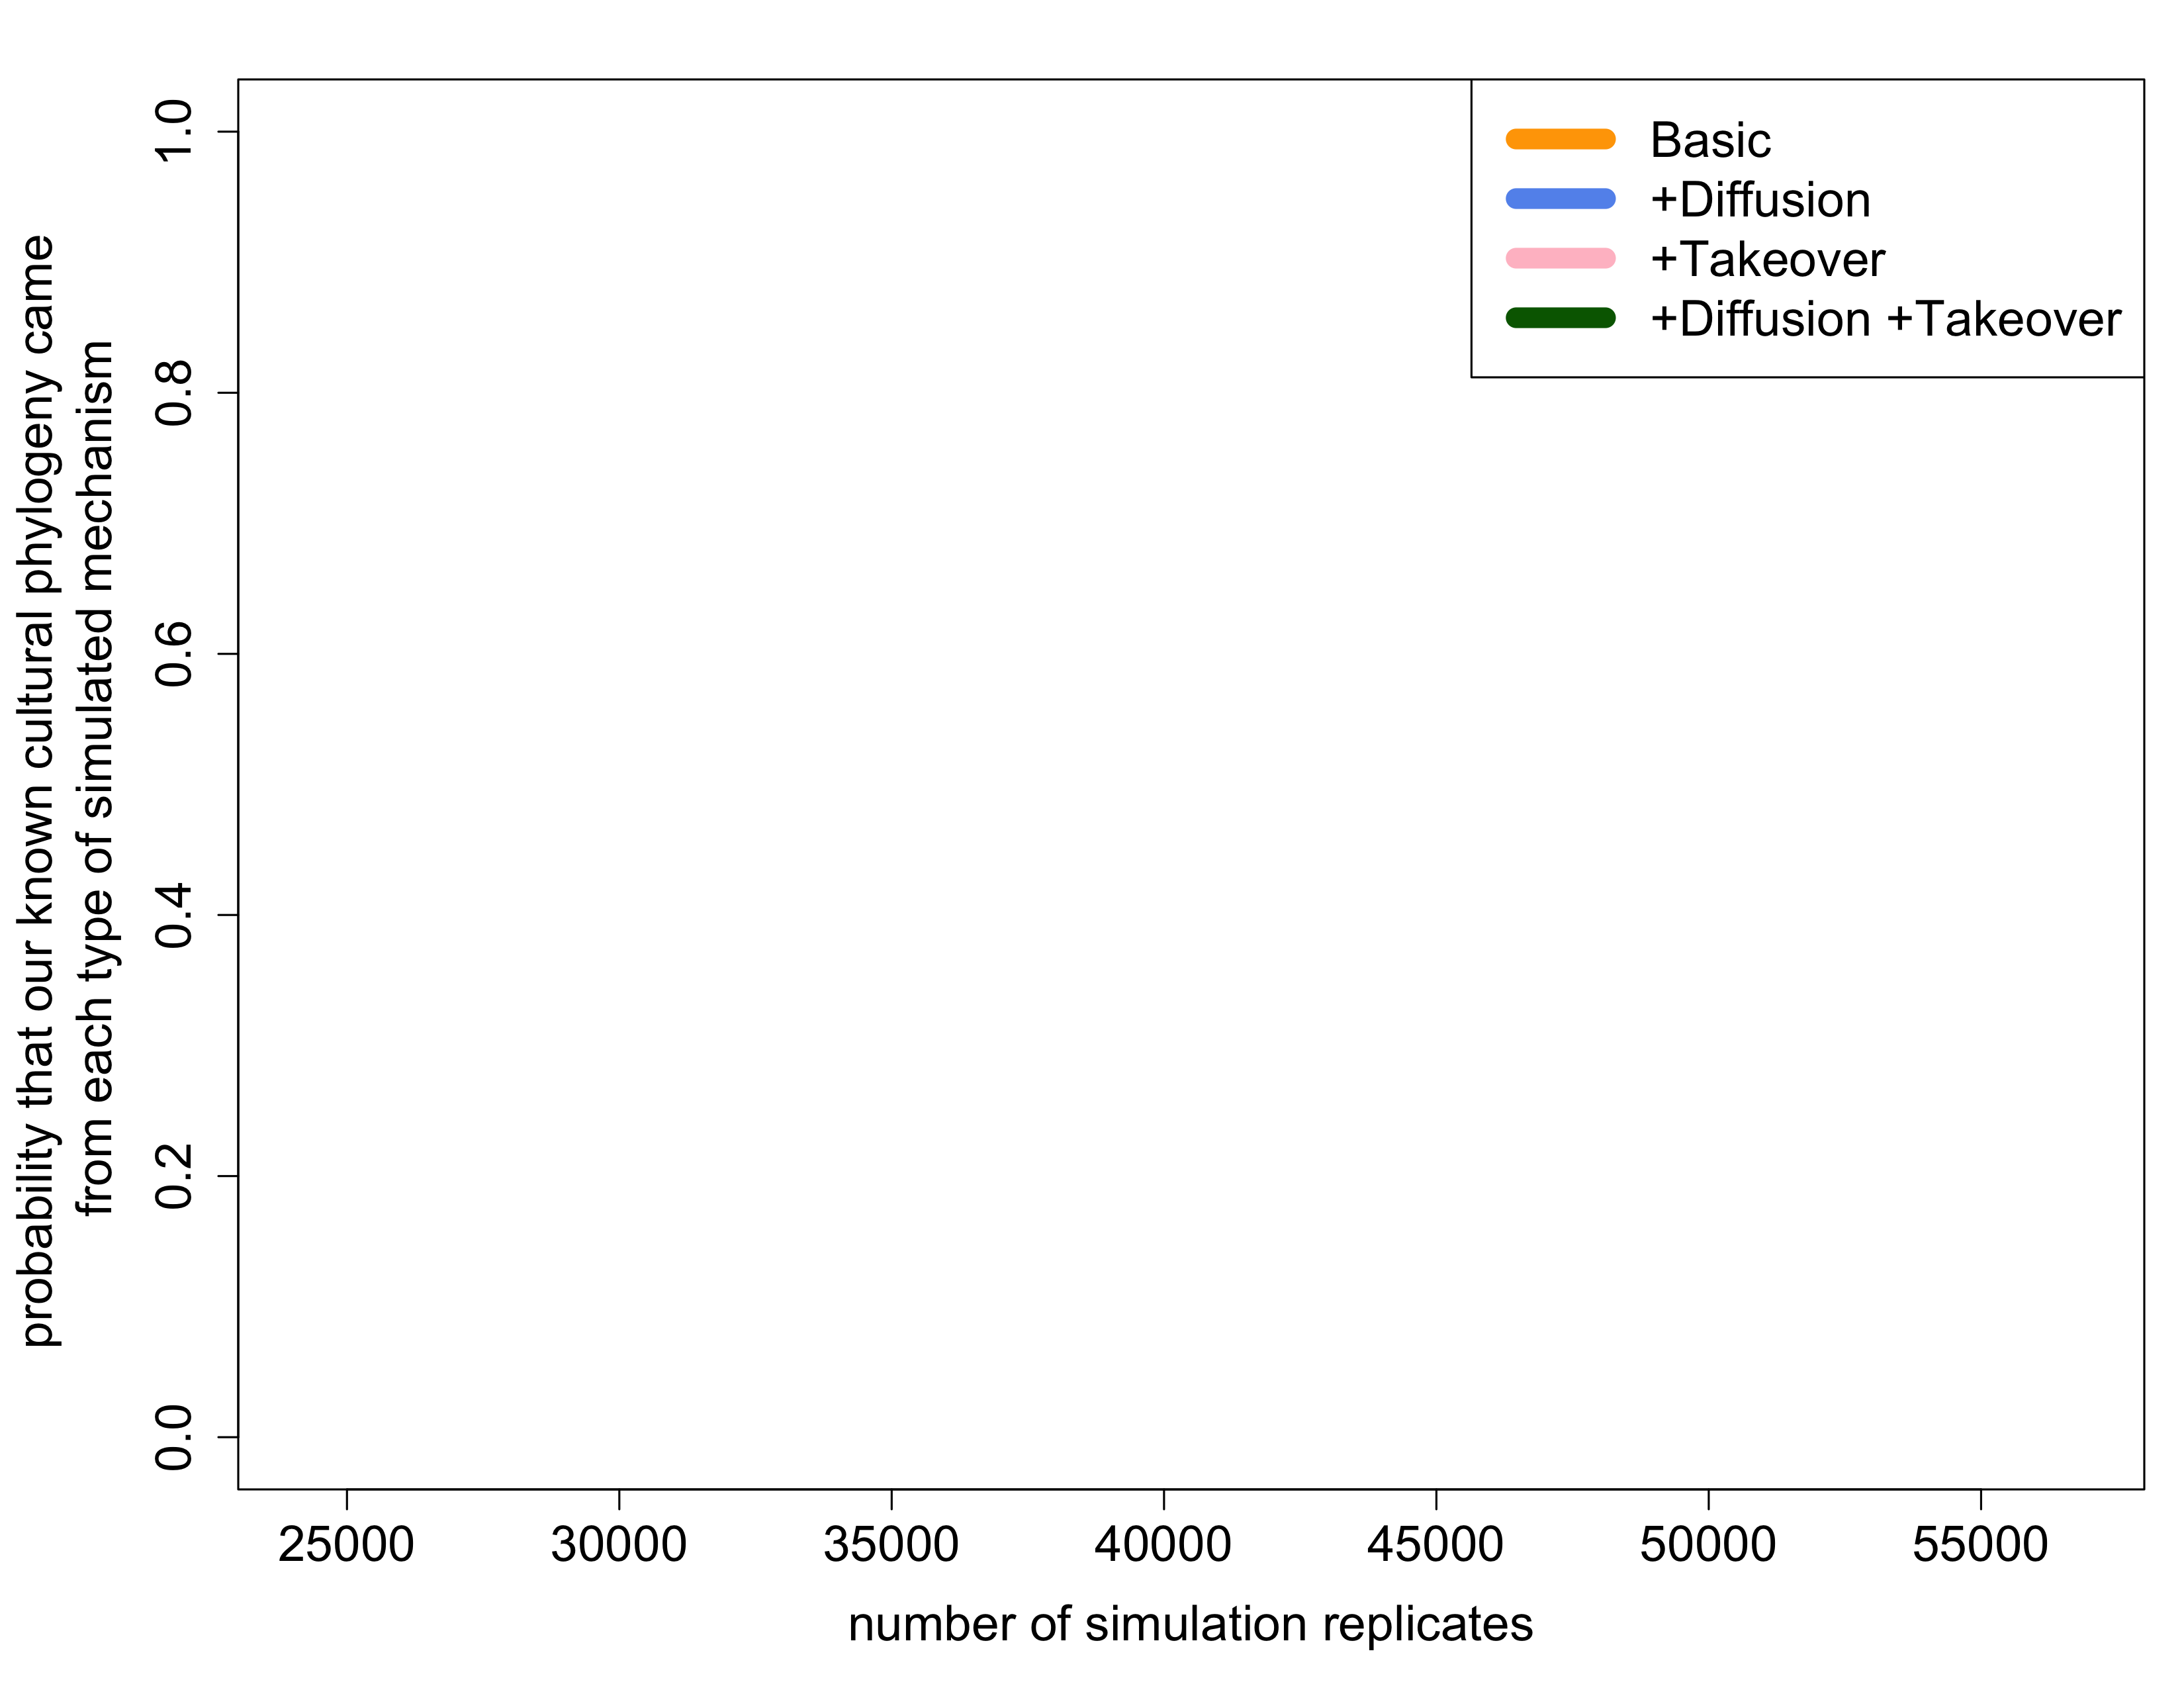
\includegraphics{predictions.png}
\caption{}
\end{figure}

\begin{Shaded}
\begin{Highlighting}[]
\KeywordTok{png}\NormalTok{(}\StringTok{"last_step_predictions.png"}\NormalTok{, }\DataTypeTok{width =} \DecValTok{11}\NormalTok{, }\DataTypeTok{height =} \FloatTok{8.5}\NormalTok{, }\DataTypeTok{res =} \DecValTok{300}\NormalTok{, }\DataTypeTok{units =} \StringTok{"in"}\NormalTok{)}
\KeywordTok{par}\NormalTok{(}\DataTypeTok{mar=}\KeywordTok{c}\NormalTok{(}\DecValTok{5}\NormalTok{,}\DecValTok{6}\NormalTok{,}\DecValTok{2}\NormalTok{,}\DecValTok{1}\NormalTok{))}
\NormalTok{this <-}\StringTok{ }\KeywordTok{length}\NormalTok{(basic_mean[,}\DecValTok{1}\NormalTok{])}

\KeywordTok{plot}\NormalTok{(}\DataTypeTok{x=}\KeywordTok{c}\NormalTok{(}\DecValTok{0}\NormalTok{,}\DecValTok{5}\NormalTok{), }\DataTypeTok{y=}\KeywordTok{c}\NormalTok{(}\DecValTok{0}\NormalTok{,}\DecValTok{1}\NormalTok{), }\DataTypeTok{type=}\StringTok{"n"}\NormalTok{,  }\DataTypeTok{xaxt=}\StringTok{"n"}\NormalTok{, }\DataTypeTok{ylab=}\StringTok{"probability that our known cultural phylogeny came }\CharTok{\textbackslash{}n}\StringTok{ from each type of simulated mechanism"}\NormalTok{, }\DataTypeTok{xlab=}\StringTok{""}\NormalTok{, }\DataTypeTok{xlim=}\KeywordTok{c}\NormalTok{(}\FloatTok{0.5}\NormalTok{,}\FloatTok{4.5}\NormalTok{))}
\KeywordTok{polygon}\NormalTok{(}\DataTypeTok{x=}\KeywordTok{c}\NormalTok{(}\FloatTok{0.75}\NormalTok{,}\FloatTok{0.75}\NormalTok{,}\FloatTok{1.25}\NormalTok{,}\FloatTok{1.25}\NormalTok{), }\DataTypeTok{y=}\KeywordTok{c}\NormalTok{(basic_mean[this,}\DecValTok{2}\NormalTok{] }\OperatorTok{-}\StringTok{ }\NormalTok{basic_sd[this,}\DecValTok{2}\NormalTok{], basic_mean[this,}\DecValTok{2}\NormalTok{] }\OperatorTok{+}\StringTok{ }\NormalTok{basic_sd[this,}\DecValTok{2}\NormalTok{], basic_mean[this,}\DecValTok{2}\NormalTok{] }\OperatorTok{+}\StringTok{ }\NormalTok{basic_sd[this,}\DecValTok{2}\NormalTok{], basic_mean[this,}\DecValTok{2}\NormalTok{] }\OperatorTok{-}\StringTok{ }\NormalTok{basic_sd[this,}\DecValTok{2}\NormalTok{]), }\DataTypeTok{col =} \KeywordTok{adjustcolor}\NormalTok{(}\StringTok{"orange"}\NormalTok{, }\DataTypeTok{alpha=}\FloatTok{0.5}\NormalTok{), }\DataTypeTok{border=}\OtherTok{NA}\NormalTok{ )}
\KeywordTok{polygon}\NormalTok{(}\DataTypeTok{x=}\KeywordTok{c}\NormalTok{(}\FloatTok{1.75}\NormalTok{,}\FloatTok{1.75}\NormalTok{,}\FloatTok{2.25}\NormalTok{,}\FloatTok{2.25}\NormalTok{), }\DataTypeTok{y=}\KeywordTok{c}\NormalTok{(diffusion_mean[this,}\DecValTok{2}\NormalTok{] }\OperatorTok{-}\StringTok{ }\NormalTok{diffusion_sd[this,}\DecValTok{2}\NormalTok{], diffusion_mean[this,}\DecValTok{2}\NormalTok{] }\OperatorTok{+}\StringTok{ }\NormalTok{diffusion_sd[this,}\DecValTok{2}\NormalTok{], diffusion_mean[this,}\DecValTok{2}\NormalTok{] }\OperatorTok{+}\StringTok{ }\NormalTok{diffusion_sd[this,}\DecValTok{2}\NormalTok{], diffusion_mean[this,}\DecValTok{2}\NormalTok{] }\OperatorTok{-}\StringTok{ }\NormalTok{diffusion_sd[this,}\DecValTok{2}\NormalTok{]), }\DataTypeTok{col =} \KeywordTok{adjustcolor}\NormalTok{(}\StringTok{"cornflowerblue"}\NormalTok{, }\DataTypeTok{alpha=}\FloatTok{0.5}\NormalTok{), }\DataTypeTok{border=}\OtherTok{NA}\NormalTok{)}
\KeywordTok{polygon}\NormalTok{(}\DataTypeTok{x=}\KeywordTok{c}\NormalTok{(}\FloatTok{2.75}\NormalTok{,}\FloatTok{2.75}\NormalTok{,}\FloatTok{3.25}\NormalTok{,}\FloatTok{3.25}\NormalTok{), }\DataTypeTok{y=}\KeywordTok{c}\NormalTok{(TO_mean[this,}\DecValTok{2}\NormalTok{] }\OperatorTok{-}\StringTok{ }\NormalTok{TO_sd[this,}\DecValTok{2}\NormalTok{], TO_mean[this,}\DecValTok{2}\NormalTok{] }\OperatorTok{+}\StringTok{ }\NormalTok{TO_sd[this,}\DecValTok{2}\NormalTok{], TO_mean[this,}\DecValTok{2}\NormalTok{] }\OperatorTok{+}\StringTok{ }\NormalTok{TO_sd[this,}\DecValTok{2}\NormalTok{], TO_mean[this,}\DecValTok{2}\NormalTok{] }\OperatorTok{-}\StringTok{ }\NormalTok{TO_sd[this,}\DecValTok{2}\NormalTok{]), }\DataTypeTok{col =} \KeywordTok{adjustcolor}\NormalTok{(}\StringTok{"pink"}\NormalTok{, }\DataTypeTok{alpha=}\FloatTok{0.5}\NormalTok{), }\DataTypeTok{border=}\OtherTok{NA}\NormalTok{)}
\KeywordTok{polygon}\NormalTok{(}\DataTypeTok{x=}\KeywordTok{c}\NormalTok{(}\FloatTok{3.75}\NormalTok{,}\FloatTok{3.75}\NormalTok{,}\FloatTok{4.25}\NormalTok{,}\FloatTok{4.25}\NormalTok{), }\DataTypeTok{y=}\KeywordTok{c}\NormalTok{(both_mean[this,}\DecValTok{2}\NormalTok{] }\OperatorTok{-}\StringTok{ }\NormalTok{both_sd[this,}\DecValTok{2}\NormalTok{], both_mean[this,}\DecValTok{2}\NormalTok{] }\OperatorTok{+}\StringTok{ }\NormalTok{both_sd[this,}\DecValTok{2}\NormalTok{], both_mean[this,}\DecValTok{2}\NormalTok{] }\OperatorTok{+}\StringTok{ }\NormalTok{both_sd[this,}\DecValTok{2}\NormalTok{], both_mean[this,}\DecValTok{2}\NormalTok{] }\OperatorTok{-}\StringTok{ }\NormalTok{both_sd[this,}\DecValTok{2}\NormalTok{]), }\DataTypeTok{col =} \KeywordTok{adjustcolor}\NormalTok{(}\StringTok{"darkgreen"}\NormalTok{, }\DataTypeTok{alpha=}\FloatTok{0.5}\NormalTok{), }\DataTypeTok{border=}\OtherTok{NA}\NormalTok{)}


\KeywordTok{lines}\NormalTok{(}\DataTypeTok{x=}\KeywordTok{c}\NormalTok{(}\FloatTok{0.5}\NormalTok{, }\FloatTok{1.5}\NormalTok{), }\KeywordTok{c}\NormalTok{(basic_mean[this,}\DecValTok{2}\NormalTok{], basic_mean[this,}\DecValTok{2}\NormalTok{]),  }\DataTypeTok{col=}\StringTok{"orange"}\NormalTok{)}
\KeywordTok{lines}\NormalTok{(}\DataTypeTok{x=}\KeywordTok{c}\NormalTok{(}\FloatTok{1.5}\NormalTok{, }\FloatTok{2.5}\NormalTok{), }\KeywordTok{c}\NormalTok{(diffusion_mean[this,}\DecValTok{2}\NormalTok{], diffusion_mean[this,}\DecValTok{2}\NormalTok{]),  }\DataTypeTok{col=}\StringTok{"cornflowerblue"}\NormalTok{)}
\KeywordTok{lines}\NormalTok{(}\DataTypeTok{x=}\KeywordTok{c}\NormalTok{(}\FloatTok{2.5}\NormalTok{, }\FloatTok{3.5}\NormalTok{), }\KeywordTok{c}\NormalTok{(TO_mean[this,}\DecValTok{2}\NormalTok{], TO_mean[this,}\DecValTok{2}\NormalTok{]),  }\DataTypeTok{col=}\StringTok{"pink"}\NormalTok{)}
\KeywordTok{lines}\NormalTok{(}\DataTypeTok{x=}\KeywordTok{c}\NormalTok{(}\FloatTok{3.5}\NormalTok{, }\FloatTok{4.5}\NormalTok{), }\KeywordTok{c}\NormalTok{(both_mean[this,}\DecValTok{2}\NormalTok{], both_mean[this,}\DecValTok{2}\NormalTok{]),  }\DataTypeTok{col=}\StringTok{"darkgreen"}\NormalTok{)}

\KeywordTok{legend}\NormalTok{(}\StringTok{"topright"}\NormalTok{, }\DataTypeTok{legend=}\NormalTok{labs, }\DataTypeTok{col=}\KeywordTok{c}\NormalTok{(}\StringTok{"orange"}\NormalTok{, }\StringTok{"cornflowerblue"}\NormalTok{, }\StringTok{"pink"}\NormalTok{, }\StringTok{"darkgreen"}\NormalTok{), }\DataTypeTok{lty=}\DecValTok{1}\NormalTok{, }\DataTypeTok{cex=}\FloatTok{1.5}\NormalTok{, }\DataTypeTok{lwd=}\DecValTok{10}\NormalTok{)}

\KeywordTok{dev.off}\NormalTok{()}
\end{Highlighting}
\end{Shaded}

\begin{figure}
\centering
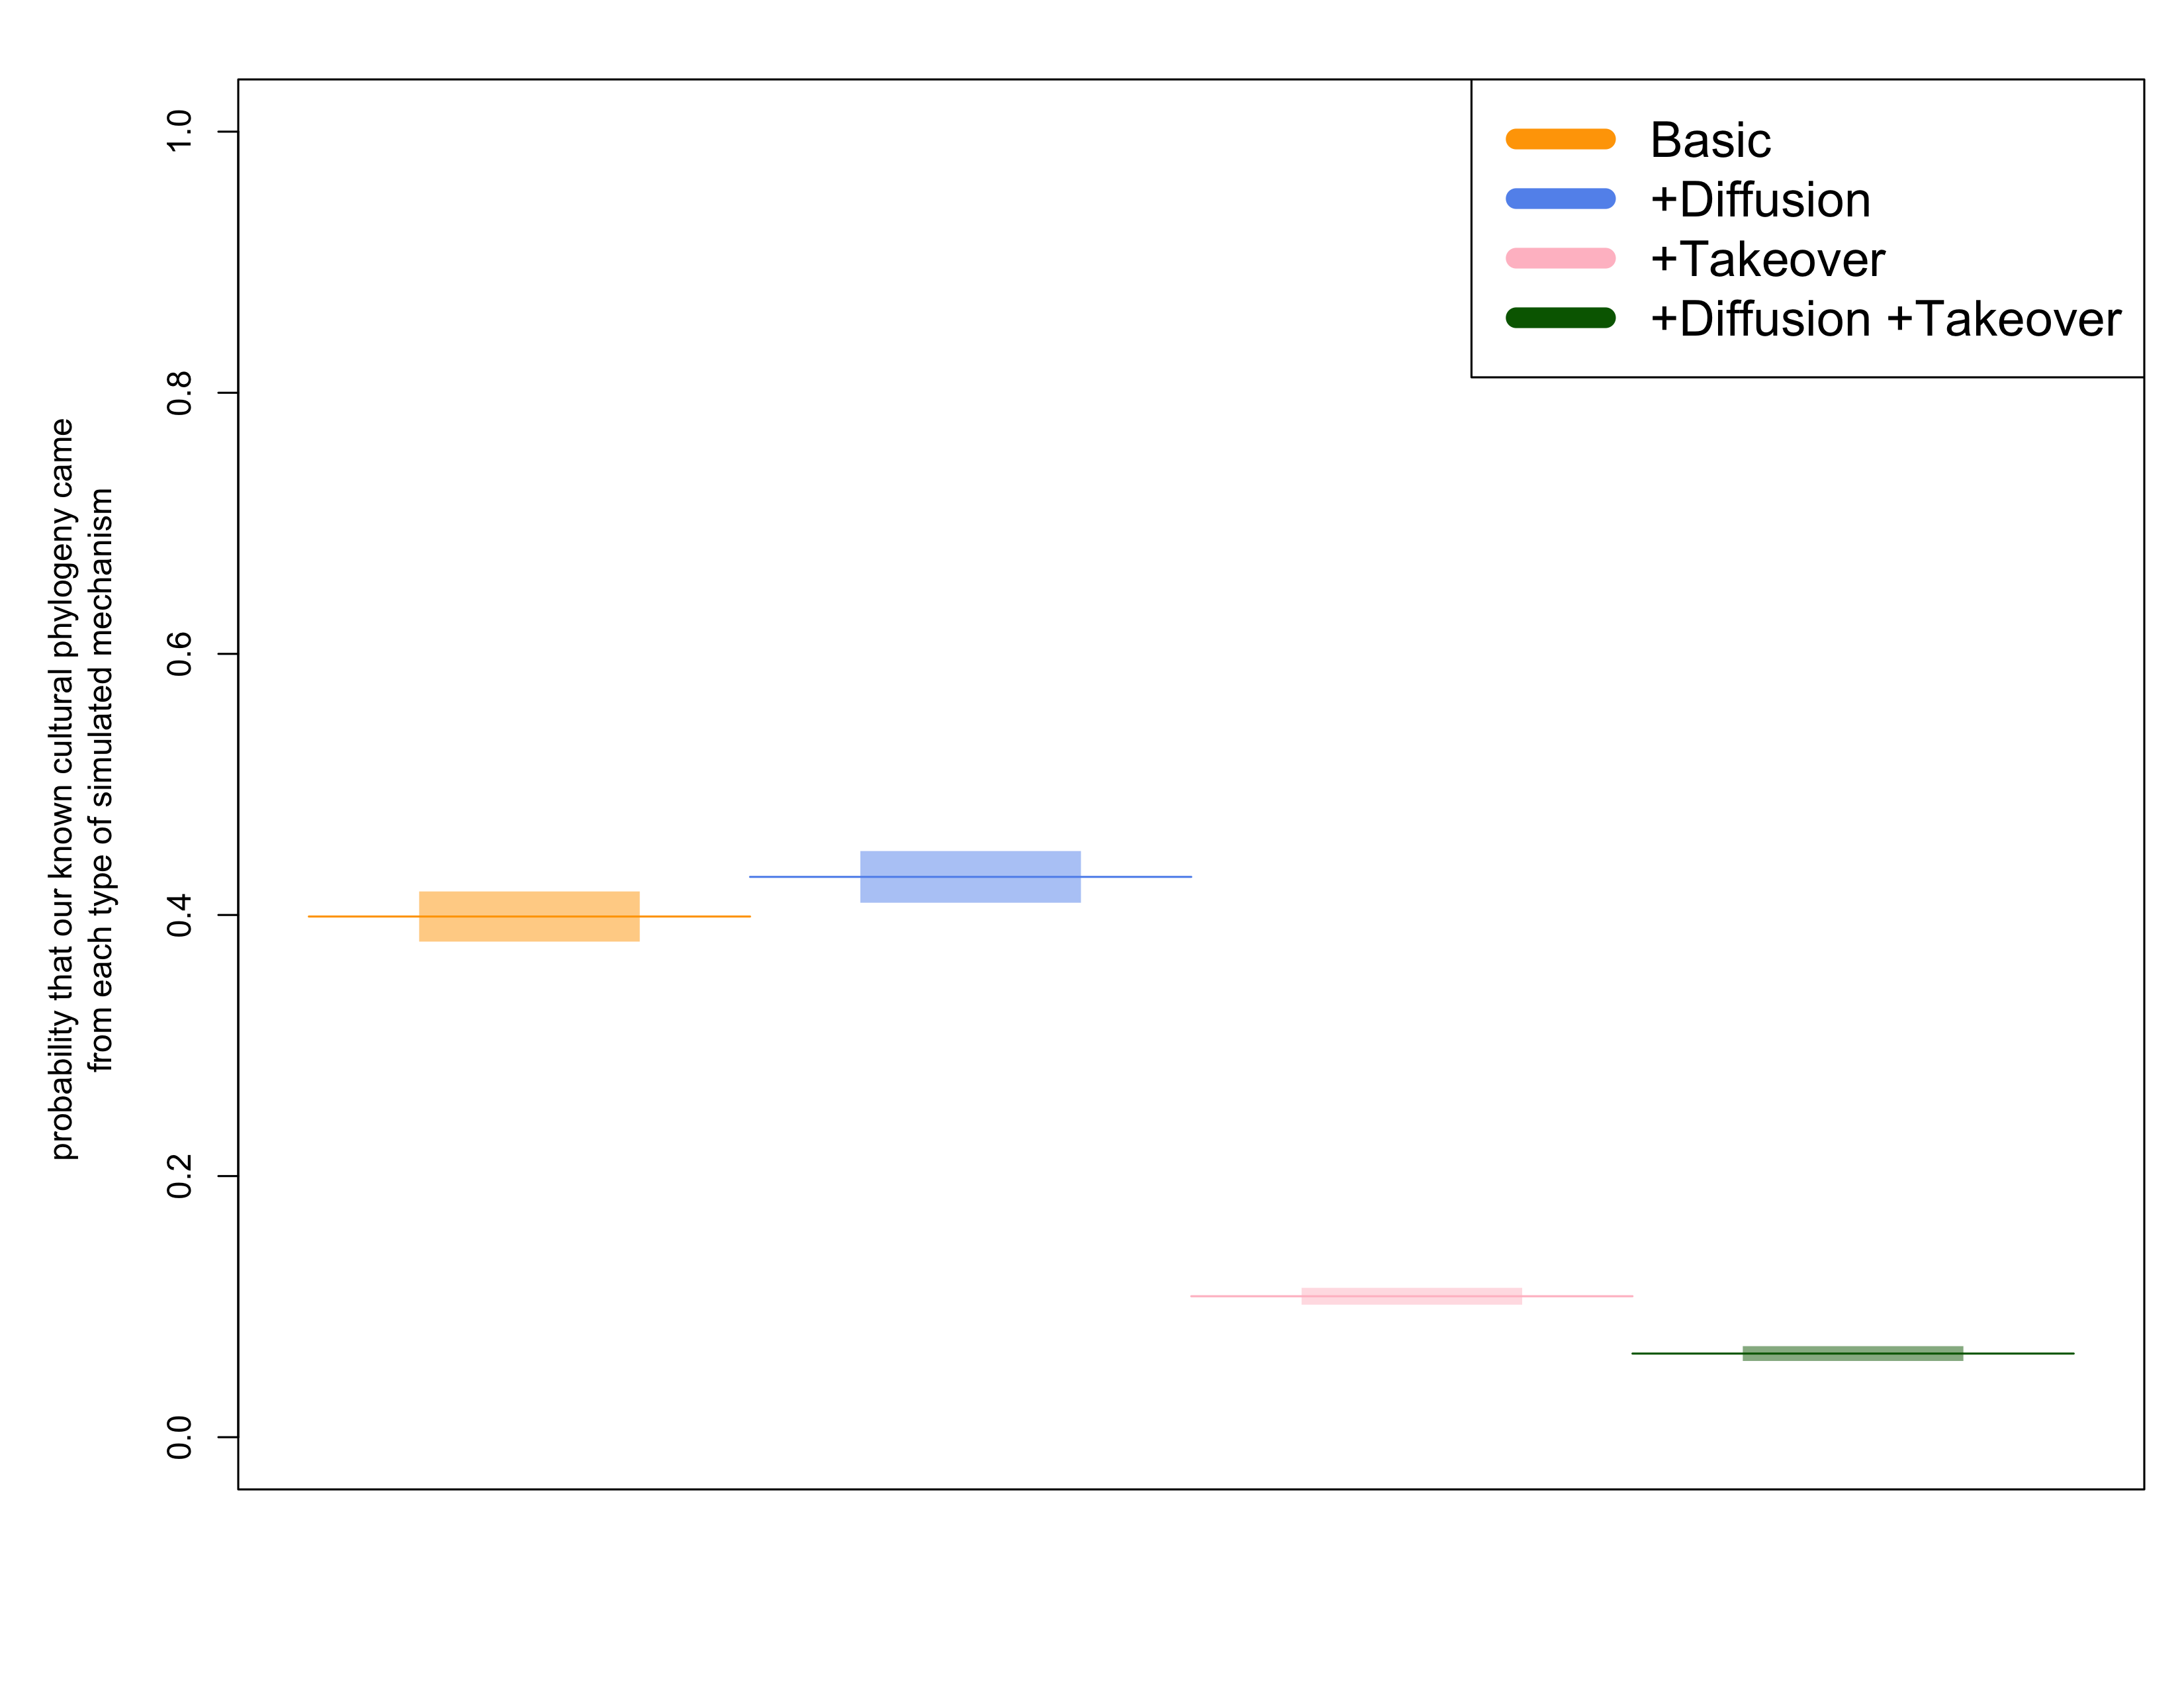
\includegraphics{last_step_predictions.png}
\caption{}
\end{figure}

\begin{Shaded}
\begin{Highlighting}[]
\CommentTok{#colnames(res_acum)}

\NormalTok{long <-}\StringTok{ }\KeywordTok{length}\NormalTok{(Confusion_0101_mean[,}\DecValTok{1}\NormalTok{])}
\NormalTok{Confusion_sum_}\DecValTok{01}\NormalTok{ <-}\StringTok{ }\KeywordTok{aggregate}\NormalTok{(}\DataTypeTok{x =}\NormalTok{ res_acum[, }\DecValTok{5}\OperatorTok{:}\DecValTok{8}\NormalTok{], }\DataTypeTok{by =} \KeywordTok{list}\NormalTok{((res_acum[, }\DecValTok{1}\NormalTok{])), }\DataTypeTok{FUN =}\NormalTok{ mean)}
\NormalTok{Confusion_sum_}\DecValTok{02}\NormalTok{ <-}\StringTok{ }\KeywordTok{aggregate}\NormalTok{(}\DataTypeTok{x =}\NormalTok{ res_acum[, }\DecValTok{9}\OperatorTok{:}\DecValTok{12}\NormalTok{], }\DataTypeTok{by =} \KeywordTok{list}\NormalTok{((res_acum[, }\DecValTok{1}\NormalTok{])), }\DataTypeTok{FUN =}\NormalTok{ mean)}
\NormalTok{Confusion_sum_}\DecValTok{03}\NormalTok{ <-}\StringTok{ }\KeywordTok{aggregate}\NormalTok{(}\DataTypeTok{x =}\NormalTok{ res_acum[, }\DecValTok{13}\OperatorTok{:}\DecValTok{16}\NormalTok{], }\DataTypeTok{by =} \KeywordTok{list}\NormalTok{((res_acum[, }\DecValTok{1}\NormalTok{])), }\DataTypeTok{FUN =}\NormalTok{ mean)}
\NormalTok{Confusion_sum_}\DecValTok{04}\NormalTok{ <-}\StringTok{ }\KeywordTok{aggregate}\NormalTok{(}\DataTypeTok{x =}\NormalTok{ res_acum[, }\DecValTok{17}\OperatorTok{:}\DecValTok{20}\NormalTok{], }\DataTypeTok{by =} \KeywordTok{list}\NormalTok{((res_acum[, }\DecValTok{1}\NormalTok{])), }\DataTypeTok{FUN =}\NormalTok{ mean)}

\NormalTok{percent_one <-}\StringTok{ }\NormalTok{(Confusion_sum_}\DecValTok{01}\NormalTok{[,}\DecValTok{2}\OperatorTok{:}\DecValTok{5}\NormalTok{]}\OperatorTok{/}\KeywordTok{sum}\NormalTok{(Confusion_sum_}\DecValTok{01}\NormalTok{[,}\DecValTok{2}\OperatorTok{:}\DecValTok{5}\NormalTok{])) }\OperatorTok{*}\StringTok{ }\DecValTok{100}
\NormalTok{percent_two <-}\StringTok{ }\NormalTok{(Confusion_sum_}\DecValTok{02}\NormalTok{[,}\DecValTok{2}\OperatorTok{:}\DecValTok{5}\NormalTok{]}\OperatorTok{/}\KeywordTok{sum}\NormalTok{(Confusion_sum_}\DecValTok{02}\NormalTok{[,}\DecValTok{2}\OperatorTok{:}\DecValTok{5}\NormalTok{])) }\OperatorTok{*}\StringTok{ }\DecValTok{100}
\NormalTok{percent_three <-}\StringTok{ }\NormalTok{(Confusion_sum_}\DecValTok{03}\NormalTok{[,}\DecValTok{2}\OperatorTok{:}\DecValTok{5}\NormalTok{]}\OperatorTok{/}\KeywordTok{sum}\NormalTok{(Confusion_sum_}\DecValTok{03}\NormalTok{[,}\DecValTok{2}\OperatorTok{:}\DecValTok{5}\NormalTok{])) }\OperatorTok{*}\StringTok{ }\DecValTok{100}
\NormalTok{percent_four <-}\StringTok{ }\NormalTok{(Confusion_sum_}\DecValTok{04}\NormalTok{[,}\DecValTok{2}\OperatorTok{:}\DecValTok{5}\NormalTok{]}\OperatorTok{/}\KeywordTok{sum}\NormalTok{(Confusion_sum_}\DecValTok{04}\NormalTok{[,}\DecValTok{2}\OperatorTok{:}\DecValTok{5}\NormalTok{])) }\OperatorTok{*}\StringTok{ }\DecValTok{100}


\NormalTok{confusion <-}\StringTok{ }\KeywordTok{matrix}\NormalTok{(}\KeywordTok{c}\NormalTok{(percent_one, percent_two, percent_three, percent_four), }\DecValTok{4}\NormalTok{,}\DecValTok{4}\NormalTok{)}

\NormalTok{labs <-}\StringTok{ }\KeywordTok{c}\NormalTok{(}\StringTok{"Basic"}\NormalTok{, }\StringTok{"+Diffusion"}\NormalTok{, }\StringTok{"+Takeover"}\NormalTok{, }\StringTok{"+Diffusion"}\NormalTok{,  }\StringTok{"+Takeover"}\NormalTok{)}
\NormalTok{colors1 <-}\StringTok{ }\KeywordTok{colorRampPalette}\NormalTok{(}\DataTypeTok{colors =} \KeywordTok{c}\NormalTok{(}\StringTok{"grey95"}\NormalTok{, }\StringTok{"grey40"}\NormalTok{))}


\KeywordTok{png}\NormalTok{(}\StringTok{"confusion_matrix.png"}\NormalTok{, }\DataTypeTok{width =} \FloatTok{8.5}\NormalTok{, }\DataTypeTok{height =} \FloatTok{8.5}\NormalTok{, }\DataTypeTok{res =} \DecValTok{600}\NormalTok{, }\DataTypeTok{units =} \StringTok{"in"}\NormalTok{)}
\KeywordTok{par}\NormalTok{(}\DataTypeTok{mar=}\KeywordTok{c}\NormalTok{(}\DecValTok{8}\NormalTok{,}\DecValTok{8}\NormalTok{,}\DecValTok{1}\NormalTok{,}\DecValTok{1}\NormalTok{))}
\KeywordTok{plot}\NormalTok{(}\DecValTok{0}\NormalTok{,}\DecValTok{0}\NormalTok{,}\DataTypeTok{xlim=}\KeywordTok{c}\NormalTok{(}\OperatorTok{-}\FloatTok{0.2}\NormalTok{,}\FloatTok{1.4}\NormalTok{), }\DataTypeTok{ylim=}\KeywordTok{c}\NormalTok{(}\OperatorTok{-}\FloatTok{0.2}\NormalTok{,}\FloatTok{1.4}\NormalTok{), }\DataTypeTok{xaxt=}\StringTok{"n"}\NormalTok{, }\DataTypeTok{xlab=}\StringTok{""}\NormalTok{, }\DataTypeTok{yaxt=}\StringTok{"n"}\NormalTok{, }\DataTypeTok{ylab=}\StringTok{""}\NormalTok{ , }\DataTypeTok{bty=}\StringTok{"n"}\NormalTok{)}
\CommentTok{#image(prop, col = colors1(20), axes=FALSE)}
\KeywordTok{axis}\NormalTok{(}\DecValTok{1}\NormalTok{, }\DataTypeTok{at=}\KeywordTok{c}\NormalTok{(}\DecValTok{0}\NormalTok{, .}\DecValTok{4}\NormalTok{, .}\DecValTok{8}\NormalTok{, }\FloatTok{1.2}\NormalTok{, }\FloatTok{1.3}\NormalTok{), }\DataTypeTok{labels=}\NormalTok{labs, }\DataTypeTok{tick =} \OtherTok{FALSE}\NormalTok{, }\DataTypeTok{line =} \OtherTok{FALSE}\NormalTok{, }\DataTypeTok{cex.axis =} \DecValTok{1}\NormalTok{, }\DataTypeTok{pos =} \OperatorTok{-}\NormalTok{.}\DecValTok{19}\NormalTok{, }\DataTypeTok{las=}\DecValTok{2}\NormalTok{)}
\KeywordTok{axis}\NormalTok{(}\DecValTok{2}\NormalTok{, }\DataTypeTok{at=}\KeywordTok{rev}\NormalTok{(}\KeywordTok{c}\NormalTok{(}\OperatorTok{-}\FloatTok{0.05}\NormalTok{, }\FloatTok{0.05}\NormalTok{, .}\DecValTok{4}\NormalTok{, .}\DecValTok{8}\NormalTok{, }\FloatTok{1.2}\NormalTok{)), }\DataTypeTok{labels=}\NormalTok{labs, }\DataTypeTok{tick =} \OtherTok{FALSE}\NormalTok{, }\DataTypeTok{line =} \OtherTok{FALSE}\NormalTok{, }\DataTypeTok{cex.axis =} \DecValTok{1}\NormalTok{, }\DataTypeTok{las=}\DecValTok{2}\NormalTok{)}
\KeywordTok{mtext}\NormalTok{(}\StringTok{"percent of time that RF identifies input model as each model type"}\NormalTok{, }\DataTypeTok{side =} \DecValTok{1}\NormalTok{, }\DataTypeTok{padj =} \DecValTok{10}\NormalTok{, }\DataTypeTok{cex =} \DecValTok{1}\NormalTok{)}
\KeywordTok{mtext}\NormalTok{(}\StringTok{"known model type given to random forest"}\NormalTok{, }\DataTypeTok{side =} \DecValTok{2}\NormalTok{, }\DataTypeTok{padj =} \OperatorTok{-}\DecValTok{10}\NormalTok{, }\DataTypeTok{cex =} \DecValTok{1}\NormalTok{)}



\ControlFlowTok{for}\NormalTok{(i }\ControlFlowTok{in} \DecValTok{1}\OperatorTok{:}\DecValTok{4}\NormalTok{) \{}
  \ControlFlowTok{for}\NormalTok{(j }\ControlFlowTok{in} \DecValTok{4}\OperatorTok{:}\DecValTok{1}\NormalTok{) \{}
\NormalTok{    xs <-}\StringTok{ }\KeywordTok{c}\NormalTok{(}\DecValTok{0}\NormalTok{, .}\DecValTok{4}\NormalTok{, .}\DecValTok{8}\NormalTok{, }\FloatTok{1.2}\NormalTok{)[i]}
\NormalTok{    ys <-}\StringTok{ }\KeywordTok{rev}\NormalTok{(}\KeywordTok{c}\NormalTok{(}\DecValTok{0}\NormalTok{, .}\DecValTok{4}\NormalTok{, .}\DecValTok{8}\NormalTok{, }\FloatTok{1.2}\NormalTok{))[j]}
    \KeywordTok{polygon}\NormalTok{(}\DataTypeTok{x=}\KeywordTok{c}\NormalTok{(xs}\OperatorTok{-}\FloatTok{0.2}\NormalTok{, xs}\OperatorTok{-}\FloatTok{0.2}\NormalTok{, xs}\OperatorTok{+}\FloatTok{0.2}\NormalTok{, xs}\OperatorTok{+}\FloatTok{0.2}\NormalTok{), }\DataTypeTok{y=}\KeywordTok{c}\NormalTok{(ys}\OperatorTok{-}\FloatTok{0.2}\NormalTok{, ys}\OperatorTok{+}\FloatTok{0.2}\NormalTok{, ys}\OperatorTok{+}\FloatTok{0.2}\NormalTok{, ys}\OperatorTok{-}\FloatTok{0.2}\NormalTok{), }\DataTypeTok{col=}\KeywordTok{colors1}\NormalTok{(}\DecValTok{100}\NormalTok{)[}\KeywordTok{round}\NormalTok{(}\KeywordTok{as.numeric}\NormalTok{(confusion[i, j]), }\DecValTok{1}\NormalTok{)}\OperatorTok{+}\DecValTok{1}\NormalTok{])}
    \ControlFlowTok{if}\NormalTok{(i }\OperatorTok{==}\StringTok{ }\NormalTok{j)\{}\KeywordTok{text}\NormalTok{(}\DataTypeTok{x =}\NormalTok{ xs, }\DataTypeTok{y =}\NormalTok{ ys, }\KeywordTok{paste0}\NormalTok{(}\KeywordTok{round}\NormalTok{(}\KeywordTok{as.numeric}\NormalTok{(confusion[i, j]), }\DecValTok{2}\NormalTok{), }\StringTok{"%"}\NormalTok{), }\DataTypeTok{cex =} \FloatTok{2.2}\NormalTok{, }\DataTypeTok{col=}\StringTok{"limegreen"}\NormalTok{)\}}\ControlFlowTok{else}\NormalTok{\{(}\KeywordTok{text}\NormalTok{(}\DataTypeTok{x =}\NormalTok{ xs, }\DataTypeTok{y =}\NormalTok{ ys, }\KeywordTok{paste0}\NormalTok{(}\KeywordTok{round}\NormalTok{(}\KeywordTok{as.numeric}\NormalTok{(confusion[i, j]), }\DecValTok{2}\NormalTok{), }\StringTok{"%"}\NormalTok{), }\DataTypeTok{cex =} \FloatTok{2.2}\NormalTok{, }\DataTypeTok{col=}\StringTok{"black"}\NormalTok{))\}}
\NormalTok{  \}}
\NormalTok{\}}
\end{Highlighting}
\end{Shaded}

\begin{figure}
\centering
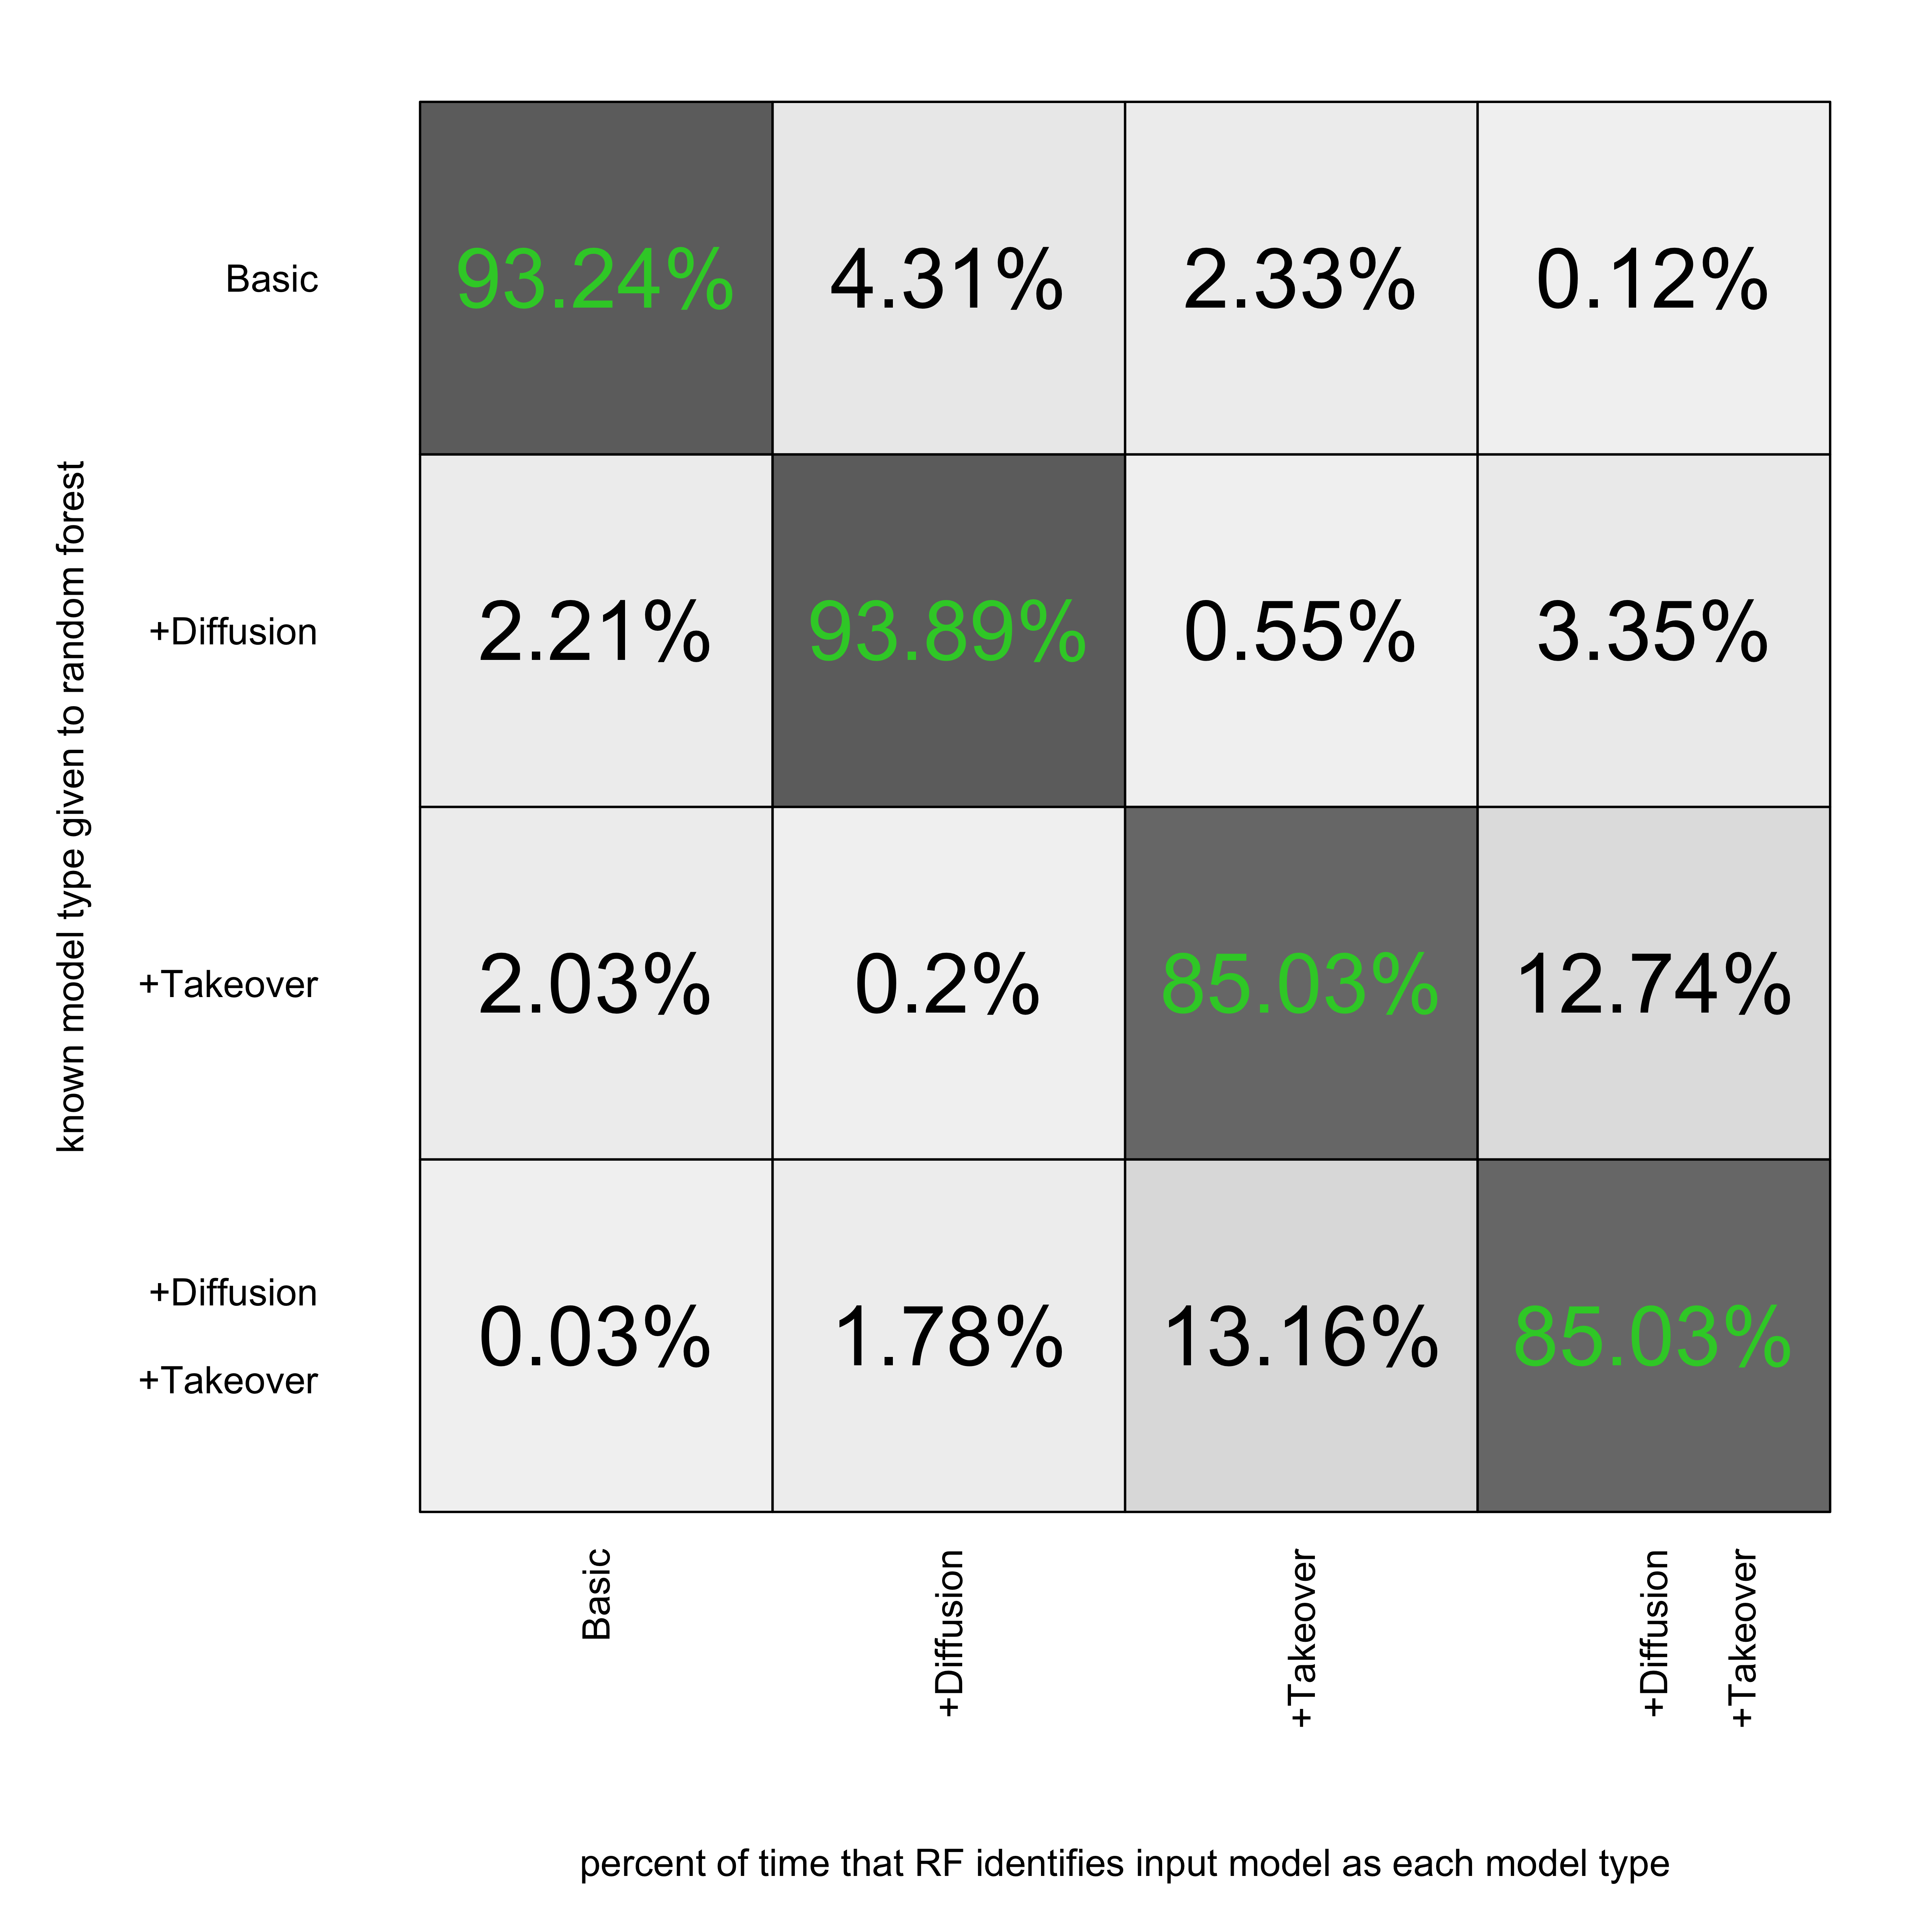
\includegraphics{confusion_matrix.png}
\caption{}
\end{figure}

\begin{Shaded}
\begin{Highlighting}[]
\CommentTok{# Variables importance}

\NormalTok{imp <-}\StringTok{ }\KeywordTok{importance}\NormalTok{(fit)}
\NormalTok{imp <-}\StringTok{ }\KeywordTok{apply}\NormalTok{(imp, }\DecValTok{2}\NormalTok{, }\ControlFlowTok{function}\NormalTok{(x) (x }\OperatorTok{-}\StringTok{ }\KeywordTok{min}\NormalTok{(x))}\OperatorTok{/}\NormalTok{(}\KeywordTok{max}\NormalTok{(x) }\OperatorTok{-}\StringTok{ }\KeywordTok{min}\NormalTok{(x)))}
\NormalTok{imp <-}\StringTok{ }\NormalTok{imp[}\KeywordTok{sort}\NormalTok{(imp[, }\DecValTok{5}\NormalTok{], }\DataTypeTok{index.return =} \OtherTok{TRUE}\NormalTok{, }\DataTypeTok{decreasing =} \OtherTok{TRUE}\NormalTok{)}\OperatorTok{$}\NormalTok{ix, ]}

\KeywordTok{as.character}\NormalTok{(replace[, }\DecValTok{6}\NormalTok{])}
\KeywordTok{load}\NormalTok{(}\KeywordTok{as.character}\NormalTok{(replace[}\DecValTok{90}\NormalTok{, }\DecValTok{6}\NormalTok{]))}
\NormalTok{imp <-}\StringTok{ }\KeywordTok{importance}\NormalTok{(fit)}

\NormalTok{names <-}\StringTok{ }\KeywordTok{rownames}\NormalTok{(imp)}
\NormalTok{names[names }\OperatorTok{==}\StringTok{ "spatial.tests.fora"}\NormalTok{] <-}\StringTok{ "Space F"}
\NormalTok{names[names }\OperatorTok{==}\StringTok{ "spatial.tests.dom"}\NormalTok{] <-}\StringTok{ "Space D"}
\NormalTok{names[names }\OperatorTok{==}\StringTok{ "sprate"}\NormalTok{] <-}\StringTok{ "Sp(ratio)"}
\NormalTok{names[names }\OperatorTok{==}\StringTok{ "transition_from_trait_1_to_2"}\NormalTok{] <-}\StringTok{ "TR(1-2)"}
\NormalTok{names[names }\OperatorTok{==}\StringTok{ "transition_from_trait_2_to_1"}\NormalTok{] <-}\StringTok{ "TR(2-1)"}
\NormalTok{names[names }\OperatorTok{==}\StringTok{ "Phylogenetic_signal"}\NormalTok{] <-}\StringTok{ "PhySig(D)"}
\NormalTok{names[names }\OperatorTok{==}\StringTok{ "Evolutionary_distinctiveness_sum"}\NormalTok{] <-}\StringTok{ "EDsum"}
\NormalTok{names[names }\OperatorTok{==}\StringTok{ "Pylo_diversity_is_sum_of_BL"}\NormalTok{] <-}\StringTok{ "PDsum"}
\NormalTok{names[names }\OperatorTok{==}\StringTok{ "transition_rate_ratio_1to2_over_2to1"}\NormalTok{] <-}\StringTok{ "TR(ratio)"}
\NormalTok{names[names }\OperatorTok{==}\StringTok{ "gamma"}\NormalTok{] <-}\StringTok{ "Gamma"}
\NormalTok{names[names }\OperatorTok{==}\StringTok{ "mean_Phylogenetic_isolation"}\NormalTok{] <-}\StringTok{ "MPI"}
\NormalTok{names[names }\OperatorTok{==}\StringTok{ "extrate"}\NormalTok{] <-}\StringTok{ "Ext(ratio)"}
\NormalTok{names[names }\OperatorTok{==}\StringTok{ "average_phylogenetic_diversity_is_mean_of_BL"}\NormalTok{] <-}\StringTok{ "PDmean"}
\NormalTok{names[names }\OperatorTok{==}\StringTok{ "extinction_per_speciation"}\NormalTok{] <-}\StringTok{ "DR"}
\NormalTok{names[names }\OperatorTok{==}\StringTok{ "variance_Phylogenetic_isolation"}\NormalTok{] <-}\StringTok{ "VPI"}
\NormalTok{names[names }\OperatorTok{==}\StringTok{ "F_quadratic_entropy_is_sum_of_PD"}\NormalTok{] <-}\StringTok{ "F"}
\NormalTok{names[names }\OperatorTok{==}\StringTok{ "Mean_pairwise_distance"}\NormalTok{] <-}\StringTok{ "MPD"}
\NormalTok{names[names }\OperatorTok{==}\StringTok{ "variance_Pylo_diversity_is_variance_of_BL"}\NormalTok{] <-}\StringTok{ "PDvar"}
\NormalTok{names[names }\OperatorTok{==}\StringTok{ "variance_pairwise_distance"}\NormalTok{] <-}\StringTok{ "VPD"}


\NormalTok{x_length <-}\StringTok{ }\KeywordTok{length}\NormalTok{(}\KeywordTok{levels}\NormalTok{(replace[,}\DecValTok{1}\NormalTok{]))}

\NormalTok{######}
\CommentTok{# make matrix}








\NormalTok{#####}
\CommentTok{#plot from matrix}










\KeywordTok{pdf}\NormalTok{(}\DataTypeTok{file=}\StringTok{"heat map of variable importance.pdf"}\NormalTok{, }\DataTypeTok{width=}\DecValTok{11}\NormalTok{, }\DataTypeTok{height=}\FloatTok{8.5}\NormalTok{)}

\KeywordTok{par}\NormalTok{(}\DataTypeTok{mar=}\KeywordTok{c}\NormalTok{(}\DecValTok{4}\NormalTok{,}\DecValTok{10}\NormalTok{,}\DecValTok{4}\NormalTok{,}\DecValTok{1}\NormalTok{))}
\KeywordTok{plot}\NormalTok{(}\DataTypeTok{x =} \KeywordTok{seq}\NormalTok{(}\DecValTok{1}\NormalTok{, x_length, }\DataTypeTok{by=}\DecValTok{1}\NormalTok{), }\DataTypeTok{y =} \KeywordTok{rep}\NormalTok{(}\DecValTok{0}\NormalTok{, x_length), }\DataTypeTok{type=}\StringTok{"n"}\NormalTok{, }\DataTypeTok{ylim=}\KeywordTok{c}\NormalTok{(}\DecValTok{0}\NormalTok{,}\DecValTok{20}\NormalTok{), }\DataTypeTok{ylab=}\StringTok{""}\NormalTok{, }\DataTypeTok{yaxt=}\StringTok{"n"}\NormalTok{, }\DataTypeTok{xaxt=}\StringTok{"n"}\NormalTok{, }\DataTypeTok{xlab=}\StringTok{""}\NormalTok{, }\DataTypeTok{xlim=}\KeywordTok{c}\NormalTok{(}\DecValTok{1}\NormalTok{, x_length}\OperatorTok{*}\DecValTok{100}\NormalTok{))}

\KeywordTok{axis}\NormalTok{(}\DecValTok{2}\NormalTok{, }\DataTypeTok{label=}\NormalTok{names, }\DataTypeTok{at=}\KeywordTok{seq}\NormalTok{(}\FloatTok{0.5}\NormalTok{,}\KeywordTok{length}\NormalTok{(names)}\OperatorTok{-}\NormalTok{.}\DecValTok{5}\NormalTok{), }\DataTypeTok{las=}\DecValTok{2}\NormalTok{)}


\ControlFlowTok{for}\NormalTok{(i }\ControlFlowTok{in} \DecValTok{1}\OperatorTok{:}\KeywordTok{length}\NormalTok{(}\KeywordTok{as.character}\NormalTok{(replace[, }\DecValTok{6}\NormalTok{])))\{}
    
    \KeywordTok{load}\NormalTok{(}\KeywordTok{as.character}\NormalTok{(replace[i, }\DecValTok{6}\NormalTok{]))}
\NormalTok{    imp <-}\StringTok{ }\KeywordTok{importance}\NormalTok{(fit)}
\CommentTok{#imp <- apply(imp, 2, function(x) (x - min(x))/(max(x) - min(x)))}
    \CommentTok{#i <- 10}
    
\NormalTok{x_range <-}\StringTok{ }\KeywordTok{c}\NormalTok{(i, i, i}\OperatorTok{+}\DecValTok{1}\NormalTok{, i}\OperatorTok{+}\DecValTok{1}\NormalTok{)    }
\NormalTok{percent <-}\StringTok{ }\KeywordTok{as.numeric}\NormalTok{(}\KeywordTok{ceiling}\NormalTok{(imp[,}\DecValTok{5}\NormalTok{] ))}
\NormalTok{percent[}\KeywordTok{which}\NormalTok{(percent }\OperatorTok{==}\StringTok{ }\DecValTok{0}\NormalTok{)] <-}\StringTok{ }\OtherTok{NA}
\NormalTok{colors <-}\StringTok{ }\KeywordTok{cm.colors}\NormalTok{(}\DecValTok{100}\NormalTok{)[percent]}

\ControlFlowTok{for}\NormalTok{(j }\ControlFlowTok{in} \DecValTok{0}\OperatorTok{:}\DecValTok{19}\NormalTok{)\{}
\NormalTok{    y_range <-}\StringTok{ }\KeywordTok{c}\NormalTok{(j, j}\OperatorTok{+}\DecValTok{1}\NormalTok{, j}\OperatorTok{+}\DecValTok{1}\NormalTok{, j)}
\KeywordTok{polygon}\NormalTok{(}\DataTypeTok{x =}\NormalTok{ x_range, }\DataTypeTok{y =}\NormalTok{ y_range, }\DataTypeTok{col=}\NormalTok{ colors[j}\OperatorTok{+}\DecValTok{1}\NormalTok{], }\DataTypeTok{border=}\OtherTok{NA}\NormalTok{)}
\NormalTok{\}}

\NormalTok{\}}

\KeywordTok{abline}\NormalTok{(}\DataTypeTok{v=}\KeywordTok{seq}\NormalTok{(}\DecValTok{0}\NormalTok{,}\DecValTok{1000}\NormalTok{, }\DataTypeTok{by=}\DecValTok{100}\NormalTok{))}

\KeywordTok{axis}\NormalTok{(}\DecValTok{1}\NormalTok{, }\DataTypeTok{label=}\KeywordTok{format}\NormalTok{(}\KeywordTok{unique}\NormalTok{(replace[,}\DecValTok{7}\NormalTok{]), }\DataTypeTok{format=}\StringTok{"%d %b %Y"}\NormalTok{), }\DataTypeTok{at=}\KeywordTok{seq}\NormalTok{(}\DecValTok{50}\NormalTok{,}\DecValTok{950}\NormalTok{, }\DataTypeTok{by=}\DecValTok{100}\NormalTok{)[}\DecValTok{1}\OperatorTok{:}\KeywordTok{length}\NormalTok{(}\KeywordTok{unique}\NormalTok{(replace[,}\DecValTok{7}\NormalTok{]))])}
\KeywordTok{dev.off}\NormalTok{()}
\end{Highlighting}
\end{Shaded}

\begin{Shaded}
\begin{Highlighting}[]
\KeywordTok{importance}\NormalTok{(fit)}
\end{Highlighting}
\end{Shaded}

\begin{Shaded}
\begin{Highlighting}[]
\CommentTok{# Variables importance}

\NormalTok{imp <-}\StringTok{ }\KeywordTok{importance}\NormalTok{(fit)}
\NormalTok{imp <-}\StringTok{ }\KeywordTok{apply}\NormalTok{(imp, }\DecValTok{2}\NormalTok{, }\ControlFlowTok{function}\NormalTok{(x) (x }\OperatorTok{-}\StringTok{ }\KeywordTok{min}\NormalTok{(x))}\OperatorTok{/}\NormalTok{(}\KeywordTok{max}\NormalTok{(x) }\OperatorTok{-}\StringTok{ }\KeywordTok{min}\NormalTok{(x)))}
\NormalTok{imp <-}\StringTok{ }\NormalTok{imp[}\KeywordTok{sort}\NormalTok{(imp[, }\DecValTok{5}\NormalTok{], }\DataTypeTok{index.return =} \OtherTok{TRUE}\NormalTok{, }\DataTypeTok{decreasing =} \OtherTok{TRUE}\NormalTok{)}\OperatorTok{$}\NormalTok{ix, ]}


\NormalTok{names <-}\StringTok{ }\KeywordTok{rownames}\NormalTok{(imp)}
\NormalTok{names[names }\OperatorTok{==}\StringTok{ "spatial.tests.fora"}\NormalTok{] <-}\StringTok{ "Space F"}
\NormalTok{names[names }\OperatorTok{==}\StringTok{ "spatial.tests.dom"}\NormalTok{] <-}\StringTok{ "Space D"}
\NormalTok{names[names }\OperatorTok{==}\StringTok{ "sprate"}\NormalTok{] <-}\StringTok{ "Sp(ratio)"}
\NormalTok{names[names }\OperatorTok{==}\StringTok{ "transition_from_trait_1_to_2"}\NormalTok{] <-}\StringTok{ "TR(1-2)"}
\NormalTok{names[names }\OperatorTok{==}\StringTok{ "transition_from_trait_2_to_1"}\NormalTok{] <-}\StringTok{ "TR(2-1)"}
\NormalTok{names[names }\OperatorTok{==}\StringTok{ "Phylogenetic_signal"}\NormalTok{] <-}\StringTok{ "PhySig(D)"}
\NormalTok{names[names }\OperatorTok{==}\StringTok{ "Evolutionary_distinctiveness_sum"}\NormalTok{] <-}\StringTok{ "EDsum"}
\NormalTok{names[names }\OperatorTok{==}\StringTok{ "Pylo_diversity_is_sum_of_BL"}\NormalTok{] <-}\StringTok{ "PDsum"}
\NormalTok{names[names }\OperatorTok{==}\StringTok{ "transition_rate_ratio_1to2_over_2to1"}\NormalTok{] <-}\StringTok{ "TR(ratio)"}
\NormalTok{names[names }\OperatorTok{==}\StringTok{ "gamma"}\NormalTok{] <-}\StringTok{ "Gamma"}
\NormalTok{names[names }\OperatorTok{==}\StringTok{ "mean_Phylogenetic_isolation"}\NormalTok{] <-}\StringTok{ "MPI"}
\NormalTok{names[names }\OperatorTok{==}\StringTok{ "extrate"}\NormalTok{] <-}\StringTok{ "Ext(ratio)"}
\NormalTok{names[names }\OperatorTok{==}\StringTok{ "average_phylogenetic_diversity_is_mean_of_BL"}\NormalTok{] <-}\StringTok{ "PDmean"}
\NormalTok{names[names }\OperatorTok{==}\StringTok{ "extinction_per_speciation"}\NormalTok{] <-}\StringTok{ "DR"}
\NormalTok{names[names }\OperatorTok{==}\StringTok{ "variance_Phylogenetic_isolation"}\NormalTok{] <-}\StringTok{ "VPI"}
\NormalTok{names[names }\OperatorTok{==}\StringTok{ "F_quadratic_entropy_is_sum_of_PD"}\NormalTok{] <-}\StringTok{ "F"}
\NormalTok{names[names }\OperatorTok{==}\StringTok{ "Mean_pairwise_distance"}\NormalTok{] <-}\StringTok{ "MPD"}
\NormalTok{names[names }\OperatorTok{==}\StringTok{ "variance_Pylo_diversity_is_variance_of_BL"}\NormalTok{] <-}\StringTok{ "PDvar"}
\NormalTok{names[names }\OperatorTok{==}\StringTok{ "variance_pairwise_distance"}\NormalTok{] <-}\StringTok{ "VPD"}


\KeywordTok{png}\NormalTok{(}\StringTok{"var_import_all.png"}\NormalTok{, }\DataTypeTok{width =} \DecValTok{25}\NormalTok{, }\DataTypeTok{height =} \DecValTok{25}\NormalTok{, }\DataTypeTok{unit=}\StringTok{"in"}\NormalTok{, }\DataTypeTok{res=}\DecValTok{300}\NormalTok{)}
\KeywordTok{par}\NormalTok{(}\DataTypeTok{mar =} \KeywordTok{c}\NormalTok{(}\DecValTok{10}\NormalTok{, }\DecValTok{18}\NormalTok{, }\DecValTok{1}\NormalTok{, }\DecValTok{1}\NormalTok{))}
\KeywordTok{plot}\NormalTok{(}\DataTypeTok{x =} \KeywordTok{rev}\NormalTok{(imp[, }\DecValTok{5}\NormalTok{]), }\DataTypeTok{y =} \DecValTok{1}\OperatorTok{:}\KeywordTok{nrow}\NormalTok{(imp), }\DataTypeTok{type =} \StringTok{"l"}\NormalTok{, }\DataTypeTok{yaxt =} \StringTok{"n"}\NormalTok{, }
     \DataTypeTok{ylab =} \StringTok{""}\NormalTok{, }\DataTypeTok{xlab =} \StringTok{"Variable Importance"}\NormalTok{,}
     \DataTypeTok{xlim =} \KeywordTok{c}\NormalTok{(}\DecValTok{0}\NormalTok{, }\DecValTok{1}\NormalTok{), }\DataTypeTok{lwd =} \DecValTok{2}\NormalTok{, }\DataTypeTok{cex.lab =} \DecValTok{4}\NormalTok{)}
\ControlFlowTok{for}\NormalTok{ (i }\ControlFlowTok{in} \DecValTok{1}\OperatorTok{:}\KeywordTok{nrow}\NormalTok{(imp)) \{}
  \KeywordTok{abline}\NormalTok{(}\DataTypeTok{h =}\NormalTok{ i, }\DataTypeTok{lty =} \DecValTok{3}\NormalTok{, }\DataTypeTok{col =} \StringTok{"gray80"}\NormalTok{)}
\NormalTok{\}}
\KeywordTok{abline}\NormalTok{(}\DataTypeTok{v =} \KeywordTok{seq}\NormalTok{(}\DecValTok{0}\NormalTok{, }\DecValTok{1}\NormalTok{, }\DecValTok{1}\OperatorTok{/}\DecValTok{19}\NormalTok{), }\DataTypeTok{lty =} \DecValTok{3}\NormalTok{, }\DataTypeTok{col =} \StringTok{"gray80"}\NormalTok{)}

\KeywordTok{lines}\NormalTok{(}\DataTypeTok{x =} \KeywordTok{rev}\NormalTok{(imp[, }\DecValTok{4}\NormalTok{]), }\DataTypeTok{y =} \DecValTok{1}\OperatorTok{:}\KeywordTok{nrow}\NormalTok{(imp), }\DataTypeTok{col =} \StringTok{"darkgreen"}\NormalTok{, }\DataTypeTok{lwd =} \DecValTok{2}\NormalTok{)}
\KeywordTok{lines}\NormalTok{(}\DataTypeTok{x =} \KeywordTok{rev}\NormalTok{(imp[, }\DecValTok{3}\NormalTok{]), }\DataTypeTok{y =} \DecValTok{1}\OperatorTok{:}\KeywordTok{nrow}\NormalTok{(imp), }\DataTypeTok{col =} \StringTok{"red"}\NormalTok{, }\DataTypeTok{lwd =} \DecValTok{2}\NormalTok{)}
\KeywordTok{lines}\NormalTok{(}\DataTypeTok{x =} \KeywordTok{rev}\NormalTok{(imp[, }\DecValTok{2}\NormalTok{]), }\DataTypeTok{y =} \DecValTok{1}\OperatorTok{:}\KeywordTok{nrow}\NormalTok{(imp), }\DataTypeTok{col =} \StringTok{"blue"}\NormalTok{, }\DataTypeTok{lwd =} \DecValTok{2}\NormalTok{)}
\KeywordTok{lines}\NormalTok{(}\DataTypeTok{x =} \KeywordTok{rev}\NormalTok{(imp[, }\DecValTok{1}\NormalTok{]), }\DataTypeTok{y =} \DecValTok{1}\OperatorTok{:}\KeywordTok{nrow}\NormalTok{(imp), }\DataTypeTok{col =} \StringTok{"darkorange1"}\NormalTok{, }\DataTypeTok{lwd =} \DecValTok{2}\NormalTok{)}
\KeywordTok{lines}\NormalTok{(}\DataTypeTok{x =} \KeywordTok{rev}\NormalTok{(imp[, }\DecValTok{5}\NormalTok{]), }\DataTypeTok{y =} \DecValTok{1}\OperatorTok{:}\KeywordTok{nrow}\NormalTok{(imp), }\DataTypeTok{lwd =} \DecValTok{3}\NormalTok{)}

\KeywordTok{points}\NormalTok{(}\DataTypeTok{x =} \KeywordTok{rev}\NormalTok{(imp[, }\DecValTok{4}\NormalTok{]), }\DataTypeTok{y =} \DecValTok{1}\OperatorTok{:}\KeywordTok{nrow}\NormalTok{(imp), }\DataTypeTok{col =} \StringTok{"darkgreen"}\NormalTok{, }\DataTypeTok{cex =} \DecValTok{2}\NormalTok{)}
\KeywordTok{points}\NormalTok{(}\DataTypeTok{x =} \KeywordTok{rev}\NormalTok{(imp[, }\DecValTok{3}\NormalTok{]), }\DataTypeTok{y =} \DecValTok{1}\OperatorTok{:}\KeywordTok{nrow}\NormalTok{(imp), }\DataTypeTok{col =} \StringTok{"red"}\NormalTok{, }\DataTypeTok{cex =} \DecValTok{2}\NormalTok{)}
\KeywordTok{points}\NormalTok{(}\DataTypeTok{x =} \KeywordTok{rev}\NormalTok{(imp[, }\DecValTok{2}\NormalTok{]), }\DataTypeTok{y =} \DecValTok{1}\OperatorTok{:}\KeywordTok{nrow}\NormalTok{(imp), }\DataTypeTok{col =} \StringTok{"blue"}\NormalTok{, }\DataTypeTok{cex =} \DecValTok{2}\NormalTok{)}
\KeywordTok{points}\NormalTok{(}\DataTypeTok{x =} \KeywordTok{rev}\NormalTok{(imp[, }\DecValTok{1}\NormalTok{]), }\DataTypeTok{y =} \DecValTok{1}\OperatorTok{:}\KeywordTok{nrow}\NormalTok{(imp), }\DataTypeTok{col =} \StringTok{"darkorange1"}\NormalTok{, }\DataTypeTok{cex =} \DecValTok{2}\NormalTok{)}
\KeywordTok{points}\NormalTok{(}\DataTypeTok{x =} \KeywordTok{rev}\NormalTok{(imp[, }\DecValTok{5}\NormalTok{]), }\DataTypeTok{y =} \DecValTok{1}\OperatorTok{:}\KeywordTok{nrow}\NormalTok{(imp), }\DataTypeTok{pch =} \DecValTok{20}\NormalTok{, }\DataTypeTok{cex =} \DecValTok{3}\NormalTok{)}


\KeywordTok{text}\NormalTok{(}\DataTypeTok{y =} \DecValTok{1}\OperatorTok{:}\KeywordTok{nrow}\NormalTok{(imp), }\DataTypeTok{x =} \KeywordTok{par}\NormalTok{(}\StringTok{"usr"}\NormalTok{)[}\DecValTok{1}\NormalTok{] }\OperatorTok{-}\StringTok{ }\NormalTok{.}\DecValTok{17}\NormalTok{, }\DataTypeTok{labels =} \KeywordTok{rev}\NormalTok{(names),}
     \DataTypeTok{srt =} \DecValTok{0}\NormalTok{, }\DataTypeTok{pos =} \DecValTok{4}\NormalTok{, }\DataTypeTok{xpd =}\NormalTok{ T, }\DataTypeTok{cex =} \DecValTok{4}\NormalTok{)}
\KeywordTok{dev.off}\NormalTok{()}
\end{Highlighting}
\end{Shaded}

\begin{figure}
\centering
\includegraphics{var_import_all.png}
\caption{}
\end{figure}

\begin{Shaded}
\begin{Highlighting}[]
\KeywordTok{par}\NormalTok{(}\DataTypeTok{mfrow=}\KeywordTok{c}\NormalTok{(}\DecValTok{2}\NormalTok{,}\DecValTok{3}\NormalTok{))}

\CommentTok{# Box plots}
\KeywordTok{boxplot}\NormalTok{(spatial.tests.fora }\OperatorTok{~}\StringTok{ }\NormalTok{Model, }\DataTypeTok{data =}\NormalTok{ data.analysis.comp3)}
\KeywordTok{abline}\NormalTok{(}\DataTypeTok{h =}\NormalTok{ a}\OperatorTok{$}\NormalTok{spatial.tests.fora, }\DataTypeTok{col =} \StringTok{"red"}\NormalTok{, }\DataTypeTok{lty =} \DecValTok{2}\NormalTok{)}

\KeywordTok{boxplot}\NormalTok{(spatial.tests.dom }\OperatorTok{~}\StringTok{ }\NormalTok{Model, }\DataTypeTok{data =}\NormalTok{ data.analysis.comp3)}
\KeywordTok{abline}\NormalTok{(}\DataTypeTok{h =}\NormalTok{ a}\OperatorTok{$}\NormalTok{spatial.tests.fora, }\DataTypeTok{col =} \StringTok{"red"}\NormalTok{, }\DataTypeTok{lty =} \DecValTok{2}\NormalTok{)}

\KeywordTok{boxplot}\NormalTok{(}\KeywordTok{log}\NormalTok{(sprate) }\OperatorTok{~}\StringTok{ }\NormalTok{Model, }\DataTypeTok{data =}\NormalTok{ data.analysis.comp3, }\DataTypeTok{ylim =} \KeywordTok{c}\NormalTok{(}\OperatorTok{-}\DecValTok{10}\NormalTok{, }\DecValTok{10}\NormalTok{))}
\KeywordTok{abline}\NormalTok{(}\DataTypeTok{h =} \KeywordTok{log}\NormalTok{(a}\OperatorTok{$}\NormalTok{sprate), }\DataTypeTok{col =} \StringTok{"red"}\NormalTok{, }\DataTypeTok{lty =} \DecValTok{2}\NormalTok{)}

\KeywordTok{boxplot}\NormalTok{(}\KeywordTok{log}\NormalTok{(extrate) }\OperatorTok{~}\StringTok{ }\NormalTok{Model, }\DataTypeTok{data =}\NormalTok{ data.analysis.comp3, }\DataTypeTok{ylim =} \KeywordTok{c}\NormalTok{(}\OperatorTok{-}\DecValTok{10}\NormalTok{, }\DecValTok{10}\NormalTok{))}
\KeywordTok{abline}\NormalTok{(}\DataTypeTok{h =} \KeywordTok{log}\NormalTok{(a}\OperatorTok{$}\NormalTok{extrate), }\DataTypeTok{col =} \StringTok{"red"}\NormalTok{, }\DataTypeTok{lty =} \DecValTok{2}\NormalTok{)}

\KeywordTok{boxplot}\NormalTok{(}\KeywordTok{log}\NormalTok{(transition_rate_ratio_1to2_over_2to1) }\OperatorTok{~}\StringTok{ }\NormalTok{Model, }\DataTypeTok{data =}\NormalTok{ data.analysis.comp3)}
\KeywordTok{abline}\NormalTok{(}\DataTypeTok{h =} \KeywordTok{log}\NormalTok{(a}\OperatorTok{$}\NormalTok{sprate), }\DataTypeTok{col =} \StringTok{"red"}\NormalTok{, }\DataTypeTok{lty =} \DecValTok{2}\NormalTok{)}

\KeywordTok{boxplot}\NormalTok{(Phylogenetic_signal }\OperatorTok{~}\StringTok{ }\NormalTok{Model, }\DataTypeTok{data =}\NormalTok{ data.analysis.comp3, }\DataTypeTok{ylim =} \KeywordTok{c}\NormalTok{(}\DecValTok{0}\NormalTok{, }\DecValTok{1}\NormalTok{))}
\KeywordTok{abline}\NormalTok{(}\DataTypeTok{h =}\NormalTok{ a}\OperatorTok{$}\NormalTok{Phylogenetic_signal, }\DataTypeTok{col =} \StringTok{"red"}\NormalTok{, }\DataTypeTok{lty =} \DecValTok{2}\NormalTok{)}
\end{Highlighting}
\end{Shaded}

\begin{Shaded}
\begin{Highlighting}[]
\CommentTok{#build a data tracking table to track parameter changes through time}

\KeywordTok{str}\NormalTok{(fit)}

\NormalTok{y}
\end{Highlighting}
\end{Shaded}

\bibliography{FARM package.bib}


\end{document}
